\chapter{Neutron Slowing Down \& Thermalization}

In the previous chapter, we covered how to solve the neutron diffusion equation using both analytical and numerical techniques, but left one major question unanswered: how do we obtain the energy spectrum to compute the group constants? The answer to this question turns out to be incredibly complicated and therefore we devote an entire chapter that honestly only gives a relative shallow treatment to the entire topic, but should hopefully provide enough foundational knowledge for an interested reader to study this topic in depth. 

Most of this chapter is devoted to the slowing down of fast neutrons from fission. On one hand, this is easier because we can actually study this question using analytical methods. On the other, the major difficulty is accounting for the effect of absorption form resonances on the neutron energy spectrum. The thermal range usually does not involve much in the way of resonances (a few notable exceptions here), but the presence of upscatter complicates matters considerably and renders analytical techniques intractable.

Qualitatively, we can break the neutron spectrum into three regions. The first two constitute the fast region, which consists of the fission and slowing down regions. The third is the thermal region. To summarize:
\begin{enumerate}
  \item Fission -- This is the portion of the fast energy range where neutrons are born from fission. It is distinguished by the fission spectrum $\chi(E) > 0$. Usually this region does not have much in the way of resonance behavior that needs to be considered. In this region, the neutron spectrum $\phi(E)$ is to a good approximation proportional to the fission spectrum. Typically the energy range is 100~keV and above.
  \item Slowing Down/Resonance -- This portion of the energy spectrum lies between the fission and thermal ranges such that $\chi(E) = 0$ (or effectively so) and that the neutron velocities are much greater than the velocities of the background nuclei such that we can neglect the effect of thermal motion and upscattering. The major feature of this region are the numerous resonances that have a large impact of the neutron spectrum. This spectrum $\phi(E)$ follows a characteristic $1/E$ shape outside the resonances with large dips in and near the resonances. Typically this range extends from about 1~eV up to 100~keV.
  \item Thermal -- This is the lower energy range where the velocities of the neutrons are comparable to the velocities of the background nuclei such that upscattering is a dominant process. Usually in this region there are few or no resonances that need to be considered. The shape of the flux spectrum $\phi(E)$ follows a Maxwellian $vM(E)$ (here $v$ is the neutron speed and $M(E)$ is the Maxwell-Boltzmann distribution) with perturbations because of the presence of absorption and leakage. Typically the thermal range is taken to be about 1~eV and below.
\end{enumerate}
We generally treat the fast regions (fission and slowing down/resonance) together using the same basic techniques and need to use different approaches for the thermal range.

Revisiting the high-level question here, the goal is to find $\phi(E)$ to compute the group constants. For reference, these are the cross sections including total, fission neutron production, and group transfer via scattering. To review, for each spatial region of the reactor, these are
\begin{subequations}
\begin{align}
  \Sigma_{tg} 
  &= \dfrac{ \displaystyle\int_g \Sigma_a(E) \phi(E) dE }{ \displaystyle\int_g \phi(E) dE }, \\
  \nu\Sigma_{fg} &= 
  \dfrac{ \displaystyle\int_g \nu \Sigma_f(E) \phi(E) dE }{ \displaystyle\int_g \phi(E) dE }, \\  
  \Sigma_{s\ell,g' \rightarrow g} &= 
  \dfrac{ \displaystyle\int_g \displaystyle\int_{g'} \Sigma_{s\ell}(E' \rightarrow E) \phi(E') dE' dE }{ \displaystyle\int_{g'}  \phi(E') dE' }.
\end{align}
\end{subequations}
Here we used the shorthand for integrating over an energy group we defined previously
\begin{align}
  \int_g \, \cdot \, dE = \int_{E_g}^{E_{g-1}} \, \cdot \, dE .
\end{align}

Here $\Sigma_{s\ell}(E' \rightarrow E )$ is the $\ell$th Legendre moment of the group scattering cross section, where $\ell = 0$ is just the differential energy-transfer cross section and $\ell = 1$ is needed to compute the group $\Sigma_{s1,g}$ from
\begin{align}
  \Sigma_{s1,g} = \sum_{g' = g}^G \Sigma_{s1,g \rightarrow g'}
\end{align}
(note the flip of the indices to sum over outgoing groups) that is needed to find the group transport cross section $\Sigma_{tr,g}$ from
\begin{align}
  \Sigma_{tr,g} = \Sigma_{t,g} - \Sigma_{s1,g} 
\end{align}
to finally compute the diffusion coefficient:
\begin{align}
  D_g = \frac{1}{3 \Sigma_{tr,g} } .
\end{align}
Note that there is some ambiguity about the ``right'' way to compute the diffusion coefficient where some references flux-weight the diffusion coefficient $D(E)$. Other references use the current spectrum $J(E)$ to weight transport cross section. For the purposes here and to avoid confusion, we will use the provided definition. Just be mindful that there are other options.

For completeness, the group removal cross section is then
\begin{align}
  \Sigma_{Rg} = \Sigma_{tg} - \Sigma_{s0,g \rightarrow g} = \Sigma_{tg} - \Sigma_{s,g \rightarrow g}.
\end{align}

Now all we need to do is walk to Mordor and compute the scalar flux spectrum $\phi(E)$, but as the old saying goes, one does not simply walk to Mordor.

%%%%%%%%%%%%%%%%%%%%%%%%%%%%%%%%%%%%%%%%%%%%%%%%%%%%%%%%%%%%%%%%%%%%%%%%%%%%%%%%%%%%%%%%%%%%%%%%%%%%
\section{Fast Neutron Elastic Scattering}

For the fast energy range of interest in reactors, most of the scattering is dominated by elastic scattering and this reaction is reasonably approximated as being isotropic in the center-of-mass frame. Making these assumptions allows us to write relatively simple expressions and perform analytical work. In reality, an actual simulation method would account for inelastic scattering, (n,2n) reactions, and anisotropy in the center-of-mass frame. We will ignore all that here, but again, be aware that this cannot be neglected for doing actual design work with computer simulations.

As we stated, we normally assume that the scattering in the center-of-mass frame is isotropic. If we let $\mu_{CM}$ be the cosine of the scattering angle in the center-of-mass frame, we have the probability density function in $\mu_{CM}$ is simply a constant from $-1$ to 1,
\begin{align}
  p(\mu_{CM}) = \frac{1}{2}, \quad -1 \le \mu_{CM} \le 1 .
\end{align}
Regardless of the form of $p(\mu_CM)$, we relate the center-of-mass scattering cosine to the lab-frame scattering cosine $\mu_0$ by using conservation of momentum and energy. For elastic scattering this is
\begin{align}
  \mu_0 = \frac{ 1 + A \mu_{CM} }{ \sqrt{ A^2 + 2 A \mu_{CM} + 1 } } .
\end{align}
Here $A$ is the atomic mass ratio: the mass of the target nucleus divided by the mass of the neutron. Using a similar analysis we can relate the center-of-mass scattering cosine to the outgoing energy $E$ given the incident energy $E'$:
\begin{align}
  E = \frac{E'}{2} \left[ ( 1 - \alpha ) \mu_{CM} + ( 1 + \alpha) \right] .
\end{align}
We refer to $\alpha$ in this context as the scattering parameter
\begin{align}
  \alpha = \left( \frac{ A - 1 }{ A + 1 } \right)^2 .
\end{align}
Note that hydrogen has $A = 1$ (or nearly so) such that $\alpha = 0$. Using these results we can derive the differential scattering cross sections in energy transfer and direction change. 

Under the assumption of scattering being isotropic in the center-of-mass frame, the differential energy-transfer cross section in the fast range (no thermal motion of the nuclei) is given by a piecewise function:
\begin{align}
  \Sigma_s(E' \rightarrow E) = \left\{ \begin{array}{l l}
  \dfrac{\Sigma_s(E')}{1-\alpha} \dfrac{1}{E'} , 	& \quad \alpha E' \le E \le E', \\
  0,												& \quad \text{otherwise}. \\ \end{array} \right.
\end{align}
Here again $E'$ is the incident energy, $E$ is the outgoing energy, and $\alpha$ is the scattering parameter.

We can derive a similar relationship for the lab-frame scattering cosine given the incident and outgoing energies. This is
\begin{align}
  \mu_0 = \mu_s( E', E ) = \left( \frac{A+1}{2} \right) \sqrt{ \frac{E}{E'} } - \left( \frac{A-1}{2} \right) \sqrt{ \frac{E'}{E} } .
\end{align}
If we inspect this result for the special case of hydrogen where $A = 1$ or $\alpha = 0$, we note that the second term vanishes. The range of $\mu_0$ is then from 0 to 1, since the minimum energy is $\alpha E' = 0$. In other words, it is impossible for a neutron to backscatter off hydrogen. For anything heavier, $A > 1$ and $\alpha > 0$, it is not too difficult to check that plugging in $E = \alpha E'$ gives $\mu_0 = -1$, which is complete backscattering. In both cases, $E = E'$, no energy transfer, corresponds to $\mu_0 = 1$, which is a glancing collision.

The double-differential elastic scattering cross section considers both energy and direction change. Because of conservation of energy and momentum needing to be conserved simultaneously, we have a one-to-one relationship between the energy transfer and the direction cosine (the azimuthal direction of scattering is uniform). To express this we have
\begin{align}
  \Sigma_s( E' \rightarrow E, \dir \cdot \dir ) = \frac{1}{2\pi} \Sigma_s(E' \rightarrow E ) \delta( \mu_0 - \mu_s(E',E) ) .
\end{align}
Note that because of the Dirac delta function, this result is consistent with setting $\mu_0 = \mu_s(E',E)$ above.

Diffusion theory can treat linearly anisotropic scattering. Therefore, it is important that we figure out the zeroth and first Legendre moments of the double-differential scattering cross section. For linearly anisotropic scattering, the double-differential scattering cross section has the Legendre polynomial expansion in lab-frame scattering cosine $\mu_0$ of
\begin{align}
  \Sigma_s( E' \rightarrow E, \dir \cdot \dir ) = \frac{1}{4\pi} \left[ \Sigma_{s0}(E' \rightarrow E ) + 3 \mu_0 \Sigma_{s1}(E' \rightarrow E) \right] .
\end{align}

If we equate these two and integrate both sides over all solid angle, we get
\begin{align}
   &\int_0^{2\pi} \int_{-1}^1 \frac{1}{2\pi} \Sigma_s(E' \rightarrow E ) \delta( \mu_0 - \mu_s(E',E) ) d\mu_0 d\gamma \nonumber \\
   &= \int_0^{2\pi} \int_{-1}^1  \frac{1}{4\pi} \left[ \Sigma_{s0}(E' \rightarrow E ) + 3 \mu_0 \Sigma_{s1}(E' \rightarrow E) \right] d\mu_0 d\gamma , \nonumber \\
   &\Sigma_s(E' \rightarrow E ) = \Sigma_{s0}(E' \rightarrow E ) .
\end{align}
This confirms an earlier result that the differential energy transfer cross section is the zeroth Legendre moment of the double-differential scattering cross section.

To get $\Sigma_{s1}(E' \rightarrow E)$, we multiply by $\mu_0$ and integrate over all solid angle. This yields
\begin{align}
   &\int_0^{2\pi} \int_{-1}^1 \frac{1}{2\pi} \Sigma_s(E' \rightarrow E ) \mu_0 \delta( \mu_0 - \mu_s(E',E) ) d\mu_0 d\gamma \nonumber \\
   &= \int_0^{2\pi} \int_{-1}^1  \frac{1}{4\pi} \left[ \Sigma_{s0}(E' \rightarrow E ) + 3 \mu_0 \Sigma_{s1}(E' \rightarrow E) \right] d\mu_0 d\gamma , \nonumber \\
   &\mu_s(E',E) \Sigma_s(E' \rightarrow E ) = \Sigma_{s1}(E' \rightarrow E ) .
\end{align}
In other words, the $\Sigma_{s1}(E' \rightarrow E)$ is the product of the differential energy-transfer scattering cross section times the direction cosine.

\subsection{Mean Energy Loss and Scattering Cosine}

Often we are interested in what happens on average in collisions. The differential energy-transfer scattering cross section times the probability density function for energy transfer. Therefore,
\begin{align}
  p( E' \rightarrow E ) = \frac{ \Sigma_s(E' \rightarrow E) }{ \Sigma_s(E') } .
\end{align}

Using this result we can compute the mean outgoing energy by multiplying this by the outgoing energy $E$ and integrating over the valid range of outgoing energies from $\alpha E'$ to $E'$. This is
\begin{align}
  \overline{E} = \int_{\alpha E'}^{E'} E p(E' \rightarrow E ) dE =  \int_{\alpha E'}^{E'} \frac{1}{1-\alpha} \frac{E}{E'} dE = \frac{1}{2} \frac{ 1 - \alpha^2 }{ 1 - \alpha } E' .
\end{align}
The mean energy loss can be found by subtracting this from the incident energy $E'$. After a little bit of algebra we can find
\begin{align}
  -\overline{ \Delta E } = \left( \frac{1 - \alpha}{2} \right) E' .
\end{align}
Note that we really did not need to take an integral to find this result, since it is just the arithmetic mean between no energy loss and the maximum energy loss. Note that this result only holds under the assumption of the scattering being isotropic in the center-of-mass frame.

To find the mean lab-frame scattering cosine, we can similarly take the integral of $\mu_s(E',E)$ times the scattering probability density and integrate over all outgoing energies. The algebra here is admittedly a bit of a slog. In the end, the result miraculously simplifies. We get
\begin{align}
  \overline{\mu}_0 = \int_{\alpha E'}^{E'} \mu_s(E',E) p(E' \rightarrow E ) dE =  \frac{2}{3A} .
\end{align}
Again, this simple result is only valid for the case of isotropic scattering in the center-of-mass frame.

The average energy loss has the largest impact on the behavior of the reactor. Neutrons do not just have one collision, but several on the path from being a fission neutron to thermalization. Unfortunately, one complication that we run into is that the average energy loss depends upon the incident energy. This means that computing the average over many collisions depends on the energy after each collision. For $n$ collisions, we would end up with an $n$-fold integral over all the possible outgoing energies. Thankfully, we can avoid doing this with a clever coordinate transformation of neutron energy into neutron lethargy.

%%%%%%%%%%%%%%%%%%%%%%%%%%%%%%%%%%%%%%%%%%%%%%%%%%%%%%%%%%%%%%%%%%%%%%%%%%%%%%%%%%%%%%%%%%%%%%%%%%%%
\section{Neutron Lethargy}

The energy loss is multiplicative process in that the amount of energy lost on each successive collision diminishes on average. When we encounter a multiplicative process, it is often beneficial to work in a logarithmic variable. We define the lethargy variable as
\begin{align}
  u = \ln\left( \frac{E_0}{E} \right) .
\end{align}
Here we take $E_0$ to the maximum plausible neutron energy of consequence in the reactor, which is typically 10-20~MeV. By this definition, all energies range from 0 up to $E_0$. In this case, the maximum energy corresponds to zero lethargy and zero energy corresponds to infinite lethargy. It follows then that energy loss corresponds to lethargy gain.

If working in the logarithmic coordinate is advantageous, we need to transfer all of our quantities to be in terms of lethargy as opposed to energy. Quantities that have a unit involving per energy such as scalar flux, current, sources, and differential energy-transfer cross sections need to be transformed to preserve the amount of a quantity (i.e., neutron path length for scalar flux) such that the amount in a differential piece of energy $dE$ is equal to the amount in a differential piece of lethargy $du$. The scalar flux, for example, transforms as
\begin{align}
  \phi(u) |du| = \phi(E) | dE | .
\end{align}
Dividing this by $|du|$, we need to take the derivative of energy with respect to lethargy. By taking the definition of lethargy and exponentiating it, we have
\begin{align}
  E = E_0 e^{-u} .
\end{align}
Differentiating with respect to $u$ gives
\begin{align}
  \frac{dE}{du} = -E_0 e^{-u} = -E .
\end{align}
Therefore, taking the absolute value, we have our coordinate transform for the scalar flux:
\begin{align}
  \phi(u) = E \phi(E) .
\end{align}
Again, the same applies to any other quantity with units of per energy.

Any quantity that does not have units of per lethargy, can simply be transformed by substituting in $u$ in terms of of $E = E_0 e^{-u}$. An example of this is a macroscopic cross section, which has units of per length, but not per energy. Therefore, a macroscopic reaction cross section transforms as
\begin{align}
  \Sigma_x(u) = \Sigma_x(E) .
\end{align} 

We are also often interested in the change in lethargy,
\begin{align}
  \Delta u = u - u' = \ln\left( \frac{E_0}{E} \right) - \ln\left( \frac{E_0}{E'} \right) = \ln\left( \frac{E'}{E} \right) .
\end{align}
For the case of neutrons losing energy, $\Delta u > 0$. One special value is the gain of one unit of lethargy. This corresponds to a neutron energy being reduced by a factor of $e^{-1}$, which corresponds to an energy loss of about 63\%.

\subsection{Differential Lethargy-Gain Cross Section}

An important quantity that needs to be transformed to be in terms of lethargy is the differential energy-transfer cross section $\Sigma_s(E' \rightarrow E)$. Applying the transformation we have for the range $\alpha E' \le E \le E'$,
\begin{align}
  \Sigma_s(u' \rightarrow u) 
  &= E \Sigma_s( E' \rightarrow E ) \nonumber \\
  &= \frac{\Sigma_s(E')}{1 - \alpha} \frac{E}{E'}  \nonumber \\
  &= \frac{\Sigma_s(u')}{1 - \alpha} \frac{E_0 e^u}{E_0 e^{u'}} \nonumber \\
  &= \frac{\Sigma_s(u')}{1 - \alpha} e^{-(u - u')} .
\end{align}
Now we need to determine the range of lethargies corresponding to the valid energy range. Using the expression for the change in lethargy, we note that the minimum energy loss of zero corresponds to no lethargy gain. The maximum energy loss corresponds to a gain of $\ln(1/\alpha)$ units of lethargy. Therefore, the valid range of lethargies following a collision with an initial lethargy of $u'$ are between $u'$ and $u'+ \ln(1/\alpha)$.

Therefore, the differential lethargy-gain cross section is
\begin{align}
  \Sigma_s(u - u') = \left\{ \begin{array}{l l}
  \dfrac{\Sigma_s(u')}{1 - \alpha} e^{-(u - u')} , 	& \quad u' \le u \le u' + \ln(1/\alpha), \\
  0,												& \quad \text{otherwise}. \\ \end{array} \right.
\end{align}
The shape of this function is a chunk of an exponential function as opposed to a spatially flat or constant function. As with energy, the probability density function for lethargy change is
\begin{align}
  p(u - u') = \frac{ \Sigma_s(u - u') }{ \Sigma_s(u') }
\end{align}
Note that these results again assume that the scattering is isotropic in the center-of-mass frame.

\subsection{Mean Lethargy Gain}

From this result, we can find the mean gain in lethargy per collision. This can be obtained by multiplying by lethargy change $u - u'$ times the probability density function and integrating over the valid range of lethargies
\begin{align}
  \overline{\Delta u} &= \xi = \int_0^{\ln(1/\alpha)} ( u - u' ) p( u - u' ) d( u - u' ) \nonumber \\
  &= 1 + \frac{ \alpha \ln(\alpha) }{ 1 - \alpha } .
\end{align}
Note we give this the conventional symbol $\xi$. This expression is a little bit of a mess in terms of $\alpha$, and there is not much we can do to simplify it. 

However, the important point here is that the mean lethargy gain during a collision is independent of the initial lethargy. This makes working out the mean lethargy gain after $n$ collisions very simple. Let this be
\begin{align}
  ( \overline{\Delta U} )_n = \overline{\Delta u}_1 + \overline{\Delta u}_2 + \ldots + \overline{\Delta u}_n .
\end{align}
Here we take $\overline{\Delta U}_n$ to be the average lethargy gain after $n$ collisions and $\overline{\Delta u}_i$ to be tbe mean lethargy change after the $i$th collision. Since $\overline{\Delta u}_i$ id independent of the initial lethargy, they are all the same value of $\xi$. Therefore we have the mean lethargy gain after $n$ collisions is simply $n$ times the mean lethargy gain per collision:
\begin{align}
  ( \overline{\Delta U} )_n = n \xi .
\end{align}

This result makes it fairly straightforward to compute the average number of collisions it takes a neutron to slow down in a particular moderator. The fewer the number of collisions required, the better the moderator. Two cases that are notable for moderators are hydrogen (the chief component of light water) and carbon, which is the element making up graphite. Suppose we wish to downscatter a neutron from 2~MeV to 1~eV. this requires a change in lethargy of
\begin{align}
  \Delta u = \ln\left( \frac{ 2 \times 10^6 \text{ eV} }{ 1 \text{ eV} } \right) = 14.5. \nonumber
\end{align}
The mean lethargy gain per collision for a neutron with hydrogen $(\alpha = 0)$ and carbon $(\alpha = 0.716)$ are
\begin{align}
  \xi^H &= 1, \nonumber \\
  \xi^C &= 0.1578. \nonumber
\end{align}
This means it requires on average 14.5 collisions for a neutron to thermalize in hydrogen and 91.9 collisions in carbon.

Of course, most materials consist of multiple isotopes with water being the key example. The question then is how one computes the mean lethargy gain for a mixture. This must be done considering both the mean lethargy gain for each particular isotope, the amount of that isotope in the mixture, and their scattering cross section. We can reason that this would be the mean lethargy gains per collision weighted by the macroscopic scattering cross sections. For a mixture we have
\begin{align}
  \xi = \dfrac{ \displaystyle\sum_i \Sigma_{s,i} \xi_i }{  \displaystyle\sum_i \Sigma_{s,i} } . \label{Eq:thermalization_meanLethargyGainMixture}
\end{align} 
Here $\Sigma_{s,i}$ is the macroscopic scattering cross section for the $i$th component and $\xi_i$ is the respective mean lethargy gain per collision. For the energy range of interest, the scattering cross section in moderating materials are mostly constant in energy, being dominated by potential scattering. Therefore, we do not need to normally worry too much about the energy dependence of the mean lethargy gain in a mixture.

Using water as an example, the microscopic scattering cross section for hydrogen is about 20~b and for oxygen it is about 4~b. With two-hydrogens per oxygen and a mean lethargy gain per collision of 1 and about 0.12 respectively. We get
\begin{align}
  \xi_{\text{H$_2$O}} = \frac{ 2 ( 20 \text{ b}) ( 1 ) + 1 ( 4 \text{ b} ) ( 0.12 ) }{ 2 ( 20 \text{ b}) + 1 ( 4 \text{ b} ) } = 0.92. \nonumber
\end{align} 

\subsection{Effectiveness of Moderators}

In assessing the effectiveness of a particular material, having a large mean lethargy gain per collision is not the only consideration. First, we need neutrons to undergo several collisions, which means the density and the scattering cross section need to be high. One measure of this is the moderating power:
\begin{align}
  \text{Moderating Power } = \xi \Sigma_s .
\end{align}

However, this is not the only condition for an effective moderator. It would not be particularly good if we successfully thermalize a bunch of neutrons only to have them absorbed within the moderator before reaching the fuel. For example, based on this metric, boron would seem to be a superior moderator compared to carbon. However, $^{10}$B has a very high neutron capture cross section, which means that most thermal neutrons would be captured before they can cause fission. 

Therefore, a better measure of the effectiveness of a moderator is given by the moderating ratio:
\begin{align}
  \text{Moderating Ratio } = &\ \frac{\text{Moderating Power}}{\text{Macroscopic Thermal Absorption Cross Section}} \nonumber \\
  = &\ \frac{ \xi \Sigma_s }{ \Sigma_a } .
\end{align}
In terms of which cross sections to use, it makes the most sense to pick $\Sigma_s$ to be the potential scattering cross section seen by fast neutrons, since we are most interested in thermalizing them. Scattering of already thermalized neutrons is perfectly, but it does not really impact the ability of the neutrons to cause fission. For the absorption cross section, it would make the most sense to pick the thermal absorption cross section. The fast absorption cross sections are very low for most (but not all) potential moderator candidates as they do not have much in the way of resonances in the slowing down range.

In terms of moderating materials available, heavy water D$_2$O is the best by a wide margin with a moderating ratio of 5670, which is mostly because deuterium has a very low absorption cross section in addition to deuterium being exceptionally light, second only to hydrogen. Light water and graphite on the other hand have moderating ratios of 71 and 192 respectively. 

So while from a pure neutron economy standpoint, heavy water is the way to go. However, from a dollar economy standpoint (heavy water is expensive), and the fact that neutron capture does happen and produces a significant quantity of radioactive tritium, we often use light water or graphite depending on the type of reactor. The advantage of light water, despite being a worse moderator than water (because hydrogen has a small, but not trivial absorption cross section) is that it is quite inexpensive and can also function as a very effective coolant. Graphite on the other hand, is a solid and must be refined to ``nuclear grade'' to eliminate boron impurities.

%%%%%%%%%%%%%%%%%%%%%%%%%%%%%%%%%%%%%%%%%%%%%%%%%%%%%%%%%%%%%%%%%%%%%%%%%%%%%%%%%%%%%%%%%%%%%%%%%%%%
\section{Slowing Down Theory}

The question we seek to answer is calculating the local neutron spectrum in the slowing down range. Here we are going to assume a uniform medium such that we can use the buckling approximation to treat leakage with the effective leakage cross section $B^2D(E)$. The source of neutrons is given by the fission spectrum $\chi(E)$ with intensity $Q_0$ neutrons per unit volume per unit time. The neutron balance equation then becomes
\begin{align}
  [ B^2 D(E) + \Sigma_t(E) ] \phi(E) = \int_0^\infty \Sigma_s(E' \rightarrow E) \phi(E') dE' + Q_0 \chi(E) . \label{Eq:thermalization_neutronBalanceEquation_Energy_General}
\end{align}

When scattering is elastic and isotropic in the center-of-mass frame, we can insert the differential energy-transfer cross section. However, in doing this we must be careful because the differential energy-transfer cross section is only non-zero over a finite range that depends on the mass of the target. To express this explicitly therefore, we need to break up the scattering term into a per-constituent basis:
\begin{align}
  \int_0^\infty \Sigma_s(E' \rightarrow E) \phi(E') dE' = \sum_i \int_E^{E/\alpha_i} \frac{\Sigma_{s,i}(E')}{1 - \alpha_i} \frac{\phi(E')}{E'} dE' .
\end{align}
Here $\alpha_i$ is the scattering parameter for the $i$th constituent. The limits of integration are over the range of possible incident energies for which a neutron scattering with a nuclide $i$ can have an outgoing energy $E$.

It is often more convenient to work in lethargy coordinates, so we then need to convert the balance relationship from $E$ to be in terms of $u$. Based on the transformation, we multiply the equation by $E$,
\begin{align}
  [ B^2 D(E) + \Sigma_t(E) ] [ E \phi(E) ] = \sum_i \int_E^{E/\alpha_i} \frac{\Sigma_{s,i}(E')}{1 - \alpha_i} \frac{E}{E'} \phi(E') dE' + Q_0 [ E \chi(E) ]. \nonumber
\end{align}
Note that $E \phi(E) = \phi(u)$, $E\chi(E) = \chi(u)$, $\Sigma_x(E) = \Sigma_x(u)$ and $D(E) = D(u)$. Also, $\phi(E) dE = -\phi(u) du$. The limits of integration transform based on the minimum incident energy $E$ going to the maximum incident lethargy $u$ and the maximum incident energy $E/\alpha$ going to $u - \ln(1/\alpha)$. After inserting the definition of lethargy in the scattering integral, we get
\begin{align}
  [ B^2 D(u) + \Sigma_t(u) ] \phi(u) = \sum_i \int_u^{u-\ln(1/\alpha_i)} \frac{\Sigma_{s,i}(u')}{1 - \alpha_i} \frac{E_0 e^{-u}}{E_0e^{-u'}} \left[ - \phi(u') du' \right] + Q_0 \chi(u) . \nonumber
\end{align}
Using the minus sign to flip the order of integration and simplifying the scattering term gives the neutron balance equation in terms of lethargy:
\begin{align}
  [ B^2 D(u) + \Sigma_t(u) ] \phi(u) = \sum_i \int_{u-\ln(1/\alpha_i)}^u \frac{e^{-(u-u')}}{1 - \alpha_i} \Sigma_{s,i}(u') \phi(u') du' + Q_0 \chi(u) . \label{Eq:thermalization_neutronBalance_MixtureLethargy}
\end{align}

This is an integral equation, which is not so easy to solve. What we will find is that we can get a solvable for the special case of hydrogen, we can solve this exactly. For heavier targets, we need to treat this approximately. In either case, to proceed we convert this into a differential equation in terms of an auxiliary quantity called the slowing down density that we introduce next.

\subsection{Slowing Down Density}

The slowing-down density $q(u)$ can be thought of as the ``flow'' rate of neutrons in energy space across some lethargy $u$. In a sense, it is analogous to the net current in neutron diffusion except in energy coordinates as opposed to spatial ones. The definition can be stated formally as the rate that neutrons, per unit volume, with lethargies in all intervals $u'$ to $u' + du'$, where $u'$ is less than some lethargy $u$, slow down via scattering into all intervals $u''$ to $u'' + du''$, where $u''$ is less than some lethargy $u$. 

This is a bit of a mouthful, so perhaps we should write down the definition mathematically and discuss it:
\begin{align}
  q(u) = \int_0^u \int_u^\infty \Sigma_s(u'' - u') \phi(u') du'' du' . \label{Eq:thermalization_slowingDensityDefinition}
\end{align}
Here $u'$ is the lethargy before the collision and $u''$ is the lethargy after the collision where we integrate over all possible collisions that take a neutron across some point in lethargy space $u$. The integrand is the scattering rate per unit lethargy for those neutrons. The inner integral is over the valid outgoing neutron lethargy range, which here are all lethargies $u'' > u$. The outer integral is over the valid incident energy range $u'$. The choice of ordering of the integrals is arbitrary, but the math tends to work out better this way.

\begin{figure}[tb!]
\begin{center}
\begin{center}
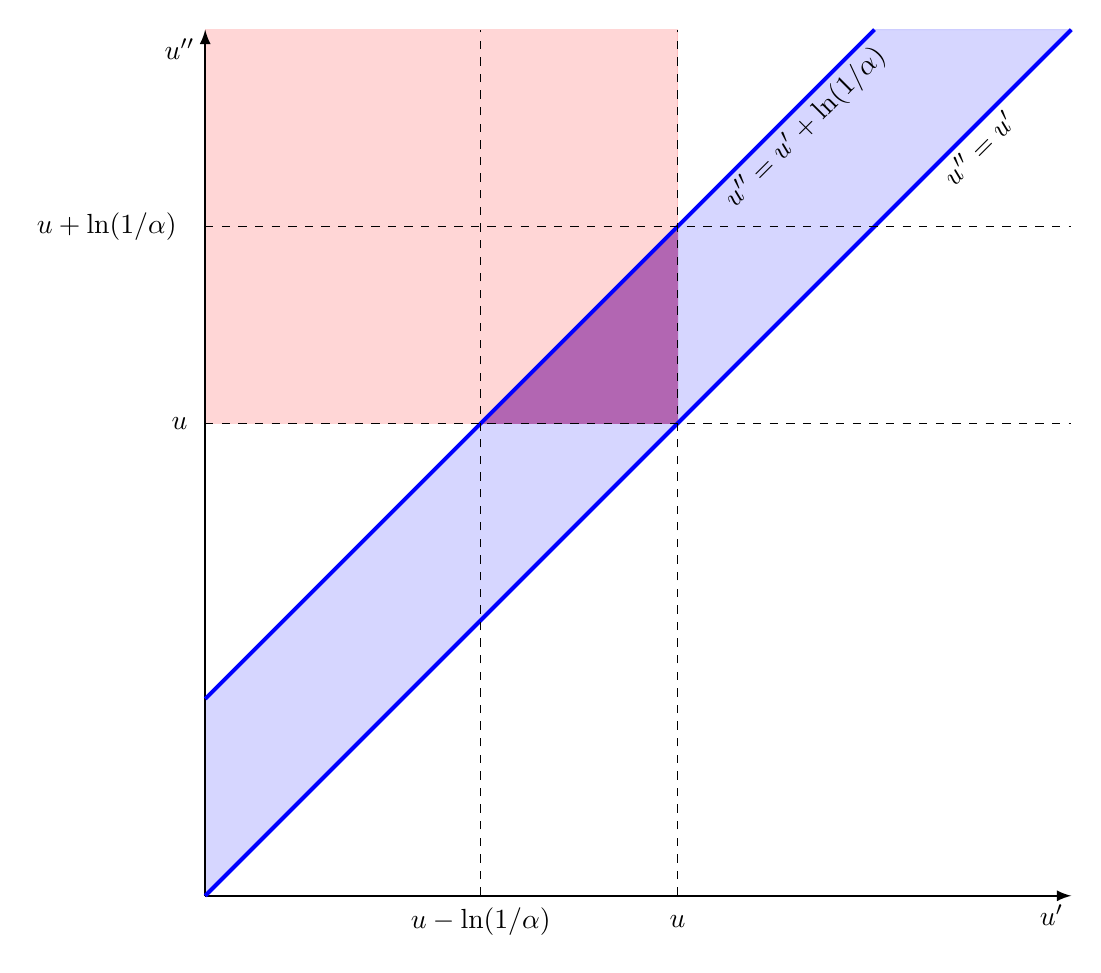
\begin{tikzpicture}
%  \fill[blue!40] (0,0) -- (4,4) -- (0,4) -- cycle;
%  \fill[red!40, decoration={random steps,segment length=0.2cm}]  (0,4) -- (4,4) -- (4,8.75) decorate{-- (0,8.75)} -- cycle;
%  \draw[-latex,thick] (0,0) -- (0,9);
%  \draw[-latex,thick] (0,0) -- (9,0);
%  \draw[dashed] (0,4) -- (4,4);
%  \draw (0,0) -- (4,4);
%  \draw[dashed] (4,0) -- (4,8.75);
%  \node at (8.75,-0.25) {$u'$};
%  \node at (-0.25,8.75) {$u''$};
%  \node at (4,-0.25) {$1$};
%  \node at (3,2.25) {$z = x$};
%  \node at (-0.25,4) {$1$}; 
  \filldraw [red!40, opacity=0.4] (0,6) -- (6,6) -- (6,11) -- (0,11) -- cycle;
  \filldraw [blue!40,opacity=0.4] (0,0) -- (11,11) -- (8.5,11) -- (0,2.5) -- cycle;
  \filldraw [violet!60] (6,6) -- (6,8.5) -- (3.5,6) -- cycle;

  \draw[-latex,thick] (0,0) -- (0,11);
  \draw[-latex,thick] (0,0) -- (11,0);
  \node at (10.75,-0.25) {$u'$};
  \node at (-0.325,10.75) {$u''$};
  
  \draw[line width=0.5mm,blue] (0,0)   -- (11,11);
  \draw[line width=0.5mm,blue] (0,2.5) -- (8.5,11);
  
  \draw[dashed] (3.5,0) -- (3.5,11);
  \draw[dashed] (6,0) -- (6,11);
  \node at (3.5,-0.325) {$u - \ln(1/\alpha)$};
  \node at (6,  -0.325) {$u$};

  \draw[dashed] (0,6) -- (11, 6);
  \draw[dashed] (0,8.5) -- (11, 8.5);
  \node at (-0.325,6) {$u$};
  \node at (-1.25,8.5) {$u + \ln(1/\alpha)$};
  
  \node[rotate = 45] at (9.825,9.5) {$u'' = u'$};
  \node[rotate = 45] at (7.625,9.75) {$u'' = u' + \ln(1/\alpha)$};
%  \draw[dashed] (8,0) -- (8,10);
\end{tikzpicture}
\end{center}
\caption{Integration Range for the Slowing Down Density}
\label{Fig:thermalization_slowingDownDensityRange}
\end{center}
\end{figure}

Here we left the differential lethargy-gain cross section ambiguous. For elastic scattering, there is only a limited range of possible lethargies for which a neutron can cross $u$ in a single scattering event for any target heavier than hydrogen. 

To find the appropriate integration domain, it is often instructive to plot the incident lethargies $u'$ versus outgoing lethargies $u''$ with respect to some lethargy $u$, which we do in Fig.~\ref{Fig:thermalization_slowingDownDensityRange}. On the horizontal $u'$ axis, we label the energetically possible incident lethargy range from $u' = u - \ln(1/\alpha)$ to $u' = u$ to cross $u$. The lower bound of this range is the smallest lethargy possible to reach $u$ because the maximum lethargy gain in a single collision is $\ln(1/\alpha)$. On the vertical $u''$ axis we denote the possible outgoing lethargies from $u$ to $u + \ln(1/\alpha)$, the latter of which is only possible if the neutron has an incident lethargy just below $u$.

We then plot two parallel lines on the plot. The first is $u'' = u'$, denoting zero lethargy gain and the second is $u'' = u' + \ln(1/\alpha)$, corresponding to the maximum lethargy gain in a collision. The region between them is shaded in blue to denote the possible lethargy transfers. For the slowing density, however, we are only interested in lethargies where $u' < u$ and $u'' > u$. This region is shaded in red. To find the integration domain, we take the intersection of these two regions; this is the triangular domain shaded in violet.

Using this integration domain, we write the slowing down density for a neutron undergoing elastic scattering as
\begin{align}
  q(u) = \int_{u'=u-\ln(1/\alpha)}^{u'=u} \int_{u''=u}^{u''=u'+\ln(1/\alpha)} \frac{e^{-(u''-u')}}{1 - \alpha} \Sigma_s(u') \phi(u') du'' du' .
\end{align}
Note that the only place that depends on $u''$ in the integrand is by way of the exponential. This allows us to carry out the integral over $u''$ explicitly to obtain
\begin{align}
  q(u) = \int_{u-\ln(1/\alpha)}^{u} \frac{e^{-(u-u')} - \alpha}{1 - \alpha} \Sigma_s(u') \phi(u') du' . \label{Eq:thermalization_slowingDownDensitySimplifed}
\end{align}
This is as far as we can take the slowing down density until we are given the scattering cross section and can solve for the scalar flux spectrum.

Before attempting to do this, we find the rate that the slowing down is changing with respect to lethargy $u$. The reason for doing this is that we will be able to write the neutron balance relationship in terms of the derivative of the slowing down density with respect to lethargy. Taking this derivative is a bit tricky since the bounds of integration involve $u$, the variable we are taking the derivative with respect to. Handling this requires the use of the Leibniz rule, which is the generalization of the second fundamental theorem of calculus:
\begin{align}
  \frac{d}{dx} \left[ \int_{a(x)}^{b(x)} f(x,y) dy \right] = f(x,b(x)) \frac{db}{dx}  - f(x,a(x)) \frac{da}{dx} + \int_{a(x)}^{b(x)} \dho{f}{x}(x,y) dy .
\end{align}
After a considerable amount of algebra, we arrive at a fairly nice result:
\begin{align}
  \frac{dq}{du} = \Sigma_s(u) \phi(u) -  \int_{u-\ln(1/\alpha)}^{u} \frac{e^{-(u-u')}}{1 - \alpha} \Sigma_s(u') \phi(u') du' . \label{Eq:thermalization_slowingDownDensityDerivative}
\end{align}

With the slowing down density and its derivative with respect to lethargy we can proceed in attempting to solve the slowing down equations. If we inspect the derivative, we see that it depends on the scattering term in the neutron balance relation. Solving for the scattering term and inserting it back into the neutron balance relation gives
\begin{align}
  [ B^2 D(u) + \Sigma_a(u) ] \phi(u) = -\frac{dq}{du} + Q_0 \chi(u) . \label{Eq:thermalization_neutronBalance_SlowingDownDensityDerivative}
\end{align}
Note that we moved the scattering term $\Sigma_s(u) \phi(u)$ to the left-hand side and wrote the loss term with absorption.

It would seem we now have written the neutron balance equation as differential equation and not an integral one in terms of the flux spectrum and derivative of the slowing down density, but there is still an integral lurking about in the slowing down density by Eq.~\eqref{Eq:thermalization_slowingDownDensitySimplifed}. It turns out we can make a key simplification for the very special case of hydrogen, which we now investigate.

\subsection{Scalar Flux Spectrum in Hydrogen}

Hydrogen is special because with $A = 1$, and therefore $\alpha = 0$, we see that a neutron can lose an arbitrary amount of energy, or equivalently gain an arbitrary amount of lethargy, in a single collision. It is also a pertinent case to analyze because hydrogen is the chief constituent in light-water that is most responsible for the moderation of neutrons, with the oxygen being significantly less important in this regard.

Setting $\alpha = 0$ in Eqs.~\eqref{Eq:thermalization_slowingDownDensitySimplifed} and~\eqref{Eq:thermalization_slowingDownDensityDerivative} for the slowing down density and its derivative, we see that the slowing down density is equal to the scattering integral of the balance relationship:
\begin{align}
  q_H(u) = \int_{u-\ln(1/\alpha)}^{u} e^{-(u-u')} \Sigma_s(u') \phi(u') du' .
\end{align}
Therefore, in this special case, we can write the derivative of the slowing down density explicitly in terms of the slowing down density itself and the scalar flux spectrum,
\begin{align}
   \frac{dq_H}{du} = \Sigma_s(u) \phi(u) - q_H(u) , \label{Eq:thermalization_slowingDownDensityDerivative_Hydrogen}
\end{align}
and then with the neutron balance equation in Eq.~\eqref{Eq:thermalization_neutronBalance_SlowingDownDensityDerivative}, we have two coupled purely differential equations by way of the derivative of the slowing down density.

Since the derivative of the slowing down density appears in both equations, we can algebraically eliminate it. This gives us a direct relationship between the scalar flux spectrum and slowing down density,
\begin{align}
  [ B^2 D(u) + \Sigma_a(u) + \Sigma_s(u) ] \phi(u) = q_H(u) + Q_0 \chi(u) . \label{Eq:thermalization_relationship_ScalarFlux_SlowingDownDensity_Hydrogen}
\end{align}
Solving for the scalar flux spectrum $\phi(u)$ and inserting this into Eq.~\eqref{Eq:thermalization_slowingDownDensityDerivative_Hydrogen} yields a first-order ordinary differential equation for just the slowing down density. We have
\begin{align}
  \frac{dq_H}{du} = \left( \frac{ B^2 D(u) + \Sigma_a(u) }{ B^2 D(u) + \Sigma_a(u) + \Sigma_s(u) } \right) q_H(u) + \left( \frac{ \Sigma_s(u) }{ B^2 D(u) + \Sigma_a(u) + \Sigma_s(u) } \right) Q_0 \chi(u).
\end{align}
Because this is a first-order differential equation we also need to infer the boundary condition at $u = 0$. By the definition of $u = 0$ corresponding to the maximum neutron energy, all neutrons are therefore born with a lethargy at or below $u = 0$. For this reason, there is no flow of neutrons downscattering past $u = 0$, so the the slowing down density is zero there,
\begin{align}
  q_H(0) = 0.
\end{align}
Note that this applies more generally than hydrogen. (A more rigorous derivation of this result involves integrating the differential equation from $-\epsilon$ to $\epsilon$ and taking the limit as $\epsilon \rightarrow 0$.)

Before we proceed with solving this, we can note that the sum of the coefficients in parentheses on the right-hand side is equal to one. The coefficient on the slowing down density is the ratio of removal events, leakage plus absorption, to all events, and the coefficient on the fission source is the ratio of scattering to all events. These are the removal and scattering probabilities respectively:
\begin{subequations}
\begin{align}
  p_R(u) &= \frac{ B^2 D(u) + \Sigma_a(u) }{ B^2 D(u) + \Sigma_a(u) + \Sigma_s(u) }, \\
  p_s(u) &= \frac{ \Sigma_s(u) }{ B^2 D(u) + \Sigma_a(u) + \Sigma_s(u) } . 
\end{align}
\end{subequations}
Therefore, we can write the differential equation for the slowing down density in a shorthand form as
\begin{align}
  \frac{dq_H}{du} = p_R(u) q_H(u) + Q_0 p_s(u) \chi(u).
\end{align}

This equation can be solved using the method of an integrating factor. Multiplying both sides by
\begin{align}
  \exp\left( -\int_0^u p_R(u') du' \right) , \nonumber
\end{align}
factorizing the left-hand side, integrating both sides of the equation from 0 to $u$, and then solving for the slowing down density gives
\begin{align}
  q_H(u) = \int_0^u Q_0 p_s(u') \chi(u') \exp\left( -\int_{u'}^u p_R(u'') du'' \right) du' . \label{Eq:thermalization_slowingDownDensity_Hydrogen_GeneralForm}
\end{align}
We should pause a moment and explain this rather complicated looking result. Starting on the left, we are integrating over all fission source neutrons emitted at lethargies $u'$ that undergo scattering with probability $p_s(u')$. The exponential term accounts for the removal of all neutrons as they are born at a lethargy $u'$ as they slow down to lethargy $u$ with a removal probability that is a function of lethargy.

Now that we have the slowing down density, we could simply insert it back into Eq.~\eqref{Eq:thermalization_relationship_ScalarFlux_SlowingDownDensity_Hydrogen} and claim victory. However, the result would not be particularly enlightening. Most of the interesting behavior is below the fission range and in the slowing down range, so we can restrict the analysis here. To start, define
\begin{align}
  u_1 = \text{ boundary between the fission and slowing down ranges.} \nonumber
\end{align}
In this case, $\chi(u) = 0$ when $u > u_1$. 

Therefore, in the slowing down region we can truncate the outer integral in Eq.~\eqref{Eq:thermalization_slowingDownDensity_Hydrogen_GeneralForm} at $u = u_1$ since there is no contribution past that point:
\begin{align}
  q_H(u) = \int_0^{u_1} Q_0 p_s(u') \chi(u') \exp\left( -\int_{u'}^u p_R(u'') du'' \right) du' , \quad u > u_1.
\end{align}
Now we can factor the exponential as
\begin{align}
   \exp\left( -\int_{u'}^u p_R(u'') du'' \right) 
   &= \exp\left( -\int_{u'}^{u_1} p_R(u'') du'' -\int_{u_1}^u p_R(u'') du''  \right) \nonumber \\
   &= \exp\left( -\int_{u'}^{u_1} p_R(u'') du'' \right) \exp\left( -\int_{u_1}^u p_R(u'') du''  \right) .\nonumber
\end{align}
Inserting this factorization into the integral and noting that the exponential on the right does not depend on the integration variable $u'$, we can pull it out of the integral. We now have
\begin{align}
  q_H(u) &= \left[ \int_0^{u_1} Q_0 p_s(u') \chi(u') \exp\left( -\int_{u'}^{u_1} p_R(u'') du'' \right) du' \right] \nonumber \\
  &\times \exp\left( -\int_{u_1}^u p_R(u') du'  \right) , \quad u > u_1.
\end{align}
Notice from Eq.~\eqref{Eq:thermalization_slowingDownDensity_Hydrogen_GeneralForm}, however, that the term in square brackets is just the slowing down density $q_H(u_1)$. Therefore, the slowing down density in the slowing down region can be written as
\begin{align}
  q_H(u) &= q_H(u_1) \exp\left( -\int_{u_1}^u p_R(u') du'  \right) , \quad u > u_1. \label{Eq:thermalization_slowingDownDensity_Hydrogen_SlowingDownRange}
\end{align}
What this is saying is that the slowing down density of neutrons in the slowing down range $u > u_1$ is the slowing down density of neutrons entering the slowing down range times an exponential attenuation factor for removal.

While that may be interesting, the scalar flux spectrum in the slowing down range is more important. Inserting this result into the neutron balance relationship in Eq.~\eqref{Eq:thermalization_relationship_ScalarFlux_SlowingDownDensity_Hydrogen} and setting $\chi(u) = 0$ for $u > u_1$, we get the result for the scalar flux spectrum:
\begin{align}
  \phi(u) = \frac{ q_H(u_1) }{ B^2 D(u) + \Sigma_a(u) + \Sigma_s(u) } \exp\left( -\int_{u_1}^u p_R(u') du'  \right) , \quad u > u_1
\end{align}
To use this, we compute the slowing down density source from the fission range and then once we have that, we can evaluate the scalar flux at any point in the slowing down range by taking the exponential of the removal probability within the slowing down range.

We can also convert this back to energy by recalling $\phi(u) = E \phi(E)$ and $du = -dE/E$. Doing the conversion gives
\begin{align}
  \phi(E) = \frac{1}{E} \frac{ q_H(E_1) }{ B^2 D(E) + \Sigma_a(E) + \Sigma_s(E) } \exp\left( -\int_E^{E_1} p_R(E') \frac{dE'}{E'}  \right) , \quad E < E_1 . \label{Eq:thermalization_fluxSpectrum_Hydrogen}
\end{align}

Note that factor of $1/E$, which may sound familiar as it is the typically flux spectrum encountered in the slowing down or resonance range when not within one of the resonances. To see this, we note that most moderators have no resonances below the fission range and negligible absorption from the $1/v$ background absorption cross section. The scattering cross section is effectively constant potential scattering in the slowing down range. Finally, if the system is large, we can neglect leakage and let $B^2 = 0$. In this case, we get the zero-removal flux spectrum as
\begin{align}
  \phi(E) =  \frac{ q_H(E_1) }{ \Sigma_s } \frac{1}{E} .
\end{align}
This is a constant divided by the energy $E$. Note that from $\phi(u) = E \phi(E)$, this implies that $\phi(u)$ is constant when there is no removal. The slowing down density is also a constant as well, which makes sense since all neutrons in the absence of leakage and absorption most eventually downscatter past a certain energy or lethargy in the slowing down range.

Note that this zero-removal result holds \emph{generally}, and not just for hydrogen. We can easily show this by plugging in this result into the neutron balance relationship in Eq.~\eqref{Eq:thermalization_neutronBalanceEquation_Energy_General}, setting the sources, leakage, and absorption to zero, and inserting the differential elastic energy-transfer scattering cross section into the equation. Carrying out the integral on the right-hand side shows that this is the correct solution for any value of $\alpha$. Therefore,
\begin{align}
  \phi(E) = \frac{C}{E} = \text{ slowing down scalar flux spectrum with no removal at energy $E$.} \nonumber
\end{align}
Here $C$ is a constant proportional to the reactor power.

The derivation we did here is not the only way of obtaining this result. In fact, most references take a different and more efficient approach of solving the integral equation by first differentiating it. The reason for not going down this route is we (1) avoided having to handle the integral equation directly and (2) we in the slowing down density and arrived at the same result using an approach that has more physical explanations to it.

Now this analysis only works for hydrogen. If we try using the approach here, we are unable to write the derivative of the slowing down density as a function of $q(u)$ as we could for hydrogen in Eq.~\eqref{Eq:thermalization_slowingDownDensityDerivative_Hydrogen}. No matter how slice it, we either are stuck with a system of equations involving an integral over the scalar flux or, should be attempt differentiating it, we then obtain something called a differential-difference equation, neither of which are solvable using analytical techniques. 

This motivates us to try one of two approaches. The first is just throw up our hands and numerically solve the integral neutron balance equation numerically on a fine lethargy grid. This has the preferred approach for quite some time, going back to at least the 1970s when computing resources became sufficiently powerful and commonly accessible to just grind through the equation. And while we could do this and get an answer, it would not necessarily tell us much about the underlying physics. The other approach involves taking a Taylor series expansion of some kind to yield an approximate form that is solvable. Broadly, these are called \emph{synthetic scattering kernel methods} because the net effect of the approximations is they, through roundabout ways, replace the mathematically problematic differential lethargy-gain cross section with one that is amenable to analytical techniques.

\subsection{Continuous-Slowing Down Approximation and Fermi Age}

The earliest attempt to analyze the slowing down of neutrons was done by Fermi during the Manhattan Project days. In this, they sought to answer the question of the leakage of fast neutrons by providing an estimate of how far a fission neutron would diffuse though a graphite moderator before thermalizing. While these approaches allowed them to design and build the earliest reactors, they are (1) not satisfactory for light moderators like water and (2) cannot provide reasonable estimates of resonance capture. Much of this section is therefore mostly of historical interest rather than practical, so we do not dwell on them, but they do allow for analytical solutions that provide insight into the slowing down process, so they are worth discussing nonetheless.

The idea begins with the slowing down density, where before we arrived at the expression
\begin{align}
  q(u) = \int_{u-\ln(1/\alpha)}^{u} \frac{e^{-(u-u')} - \alpha}{1 - \alpha} \Sigma_s(u') \phi(u') du' .
\end{align}
The problem here is that the presence of $\Sigma_s(u') \phi(u')$ makes the integral impossible to do directly (except for hydrogen as we just showed). The trick here is to take a \emph{zeroth-order Taylor series expansion} of this term about $u' = u$:
\begin{align}
  \Sigma_s(u') \phi(u') \approx \Sigma_s(u) \phi(u) .
\end{align}

This may seem laughable, but remember Fermi and his team were on a tight schedule and did not have computers to help them out. The consequence of this approximation is these equations are only accurate to order $1/A$, which means that they are only applicable for heavy moderators. Plugging this approximation into the slowing down density, allows us to pull the scattering rate out of the integral and evaluate it to obtain
\begin{align}
  q(u) = \xi \Sigma_s(u) \phi(u) . \label{Eq:thermalization_slowingDownDensity_AgeTheory}
\end{align}
This says the slowing down density is approximately the moderating power times the scalar flux.

With such a simple relationship, we can solve for $\phi(u)$ in terms of $q(u)$ and insert it into the neutron balance relationship in Eq.~\eqref{Eq:thermalization_neutronBalance_SlowingDownDensityDerivative}. We will also go back a stop and apply the buckling relation $\nabla^2 \phi = -B^2 \phi$ to write this as s function of space as well as lethargy:
\begin{align}
  \dho{q}{u} - \frac{D(u)}{\xi \Sigma_s(u)} \nabla^2 q(\pos,u) + \frac{\Sigma_a(u)}{\xi \Sigma_s(u)} q(\pos,u) = Q(\pos) \chi(u) . \label{Eq:thermalization_continuousSlowingDown_SlowingDownDensityDiffusionEqn}
\end{align}
As we saw in the analysis for hydrogen with Eq.~\eqref{Eq:thermalization_slowingDownDensity_Hydrogen_SlowingDownRange}, if we are only concerned with the slowing down region where $\chi(u) = 0$, we can write the solution using an ``initial condition'' at the top of the slowing down range that describes the source. The form of $\chi(u)$ does not matter, so we replace it with a Dirac delta function and take $u = 0$ to be the top of the slowing down region. We can introduce a transformation involving the integrating factor
\begin{align}
  \widetilde{q}(\pos,u) = q(\pos,u) \exp\left( \int_0^u \frac{\Sigma_a(u')}{\xi \Sigma_s(u')} du'  \right),
\end{align}
which allows us to eliminate the reaction term and write the diffusion equation as
\begin{align}
  \dho{\widetilde{q}}{u} - \frac{D(u)}{\xi \Sigma_s(u)} \nabla^2 \widetilde{q}(\pos,u) = Q(\pos) \delta(u) .
\end{align}

This equation looks very similar the classic time-dependent diffusion problem where $u$ is a time-like variable. The rationale for doing this is that this particular equation has well known solution techniques---these were very well understood at the time Fermi was making them.

We now make one more transformation using the coefficient on $\nabla^2 \widetilde{q}$ and define the \emph{Fermi age}:
\begin{align}
  \tau = \int_0^u \frac{D(u')}{\xi\Sigma_s(u')} du' .
\end{align}
The Fermi age is another time-like variable that is an elongated lethargy variable, but with units of area. This particular transformation allows for describing the migration length of fast neutrons, which is the real motivator for the choice.

We then transform $u \rightarrow \tau$ to get
\begin{align}
  \dho{\widetilde{q}}{\tau} - \nabla^2 \widetilde{q}(\pos,\tau) = Q(\pos) \delta(\tau) .
\end{align}
If we consider the special case where the source is localized to a single location $\pos_0 = (x_0,y_0,z_0)$ that we describe with the Dirac delta function,
\begin{align}
  Q(\pos) = Q_0 \delta( x - x_0 ) \delta( y - y_0 ) \delta( z - z_0 ),
\end{align}
and an infinite medium, this equation has a well-known solution of a Gaussian that spreads out in ``time'' or Fermi age:
\begin{align}
  \widetilde{q}_0(\pos,\tau) = \frac{1}{(4 \pi \tau)^{3/2}} \exp\left( -\frac{r^2}{4\tau} \right) .
\end{align}
Here $r$ is the distance between a point $\pos$ and the source point $\pos_0$. (We denote this quantity with a zero subscript to delineate it as being for a point source.) In fact this solution is the Green's function and we can, at least numerically, solve for the transformed slowing down density any source distribution $Q(x)$ by integrating over all the source points. The actual slowing down density can be obtained by reversing the transformation from $\widetilde{q} \rightarrow q$ and putting the integral in terms of the Fermi age. This keeps the same overall shape, but exponentially attenuates as the Fermi age increases because of leakage and absorption. The shape here confirms what we would expect, that neutrons born from fission at a localized point will spread out as they slow down. This result explains precisely how.

\subsubsection{Migration Area Revisited}

We can use this result to predict how far fast neutrons migrate to thermalization. We can calculate the root-mean square distance to thermalization as a function of the Fermi age, $\tau$. This mean-square distance is
\begin{align}
  \overline{r^2} = \dfrac{ \displaystyle\int_0^\infty 2\pi r^2 \widetilde{q}_0(r,\tau) r^2 dr }{ \displaystyle\int_0^\infty 2\pi \widetilde{q}_0(r,\tau) r^2 dr } = \frac{ 3\tau }{1/2} = 6\tau .
\end{align}

Recalling $\tau$ has units of area, this result may look similar to what we obtained in Sec.~\ref{Sec:neutronics_DiffusionMigrationDistance} from one-speed diffusion theory that the mean-square distance is equal to $6 L^2$. This allows us to define the migration area in terms of the Fermi aga. Suppose we use Fermi age theory to handle the fast migration and one-speed diffusion theory to find the thermal migration. Taking the sum of the squares of the distances gives the migration distance for neutrons born from fission, through thermalization, and ultimately until absorption. We then express the migration area as the sum of the Fermi age $\tau$ plus the thermal diffusion length $L$ squared:
\begin{align}
  M^2 = \tau + L^2 .
\end{align}

\subsubsection{Fast Non-Leakage Probability}

Another result using the Fermi age is the fast non-leakage probability $P_{FNL}$. A simple model for this is that of a zero-temperature reactor such that by definition all neutrons are fast and we can completely ignore thermalization. (We know that reactors obviously operate at a finite temperature, but this allows for getting a clean result for the fast neutrons.) We also assume as before that all neutrons are produced at lethargy $u = 0$. 

The neutron balance equation for the criticality problem can be expressed as
\begin{align}
  [ B^2 D(u) + \Sigma_a(u) ] \phi(u) = -\frac{dq}{du} + \frac{1}{k} \delta(u) \int_0^\infty \nu\Sigma_f(u') \phi(u') du'. 
\end{align}
Here we also assume a spatially homogeneous medium so that we can apply the buckling approximation. 

Applying the continuous-slowing down approximation, we have from Eq.~\eqref{Eq:thermalization_slowingDownDensity_AgeTheory} that the slowing down density is simply the moderating power times the scalar flux spectrum. Multiplying and dividing the left-hand side by the scattering cross section, we can write a first-order ordinary differential equation for the scattering density $\Sigma_s(u) \phi(u)$,
\begin{align}
  \frac{d}{du} [ \Sigma_s(u) \phi(u) ] + \left( \frac{B^2 D(u) + \Sigma_a(u)}{\xi \Sigma_s(u)} \right) [ \Sigma_s(u) \phi(u) ] = \frac{1}{k \xi} \delta(u) \int_0^\infty \nu\Sigma_f(u') \phi(u') du'. 
\end{align}
Note that the right-hand side only depends on the variable $u$ by way of the Dirac delta function where the integral results in a constant, which we denote as
\begin{align}
  Q_0 = \int_0^\infty \nu\Sigma_f(u') \phi(u') du'.
\end{align}

We can then solve this equation for the scalar flux spectrum using the integrating factor. The result of this calculation is
\begin{align}
  \phi(u) = \frac{ Q_0 }{ k \xi \Sigma_s(u) } \exp\left[ -\int_0^u \frac{B^2 D(u') + \Sigma_a(u')}{\xi \Sigma_s(u')} du' \right]
\end{align}
We can solve for $k$ by multiplying both sides by $\nu\Sigma_f(u)$ and integrating over all lethargies:
\begin{align}
  k \int_0^\infty \nu\Sigma_f(u) \phi(u) &= \int_0^u \nu\Sigma_f(u) \frac{ Q_0 }{ \xi \Sigma_s(u) } \exp\left[ -\int_0^u \frac{B^2 D(u') + \Sigma_a(u')}{\xi \Sigma_s(u')} du' \right] du, \nonumber \\
  k Q_0 &= Q_0 \int_0^\infty  \frac{ \nu\Sigma_f(u)}{ \xi \Sigma_s(u) } \exp\left[ -\int_0^u \frac{B^2 D(u') + \Sigma_a(u')}{\xi \Sigma_s(u')} du' \right] du , \nonumber \\
  k &= \int_0^\infty  \frac{ \nu\Sigma_f(u)}{ \xi \Sigma_s(u) } \exp\left[ -\int_0^u \frac{B^2 D(u') + \Sigma_a(u')}{\xi \Sigma_s(u')} du' \right] du
\end{align}

We can put this in terms of the Fermi age by breaking up the sum of the exponentials as a product of exponentials
\begin{align}
  k &= \int_0^\infty  \frac{ \nu\Sigma_f(u)}{ \xi \Sigma_s(u) } \exp\left[ -\int_0^u \frac{\Sigma_a(u')}{\xi \Sigma_s(u')} du' \right] \exp\left[ -\int_0^u \frac{B^2 D(u')}{\xi \Sigma_s(u')} du'  \right]  du \nonumber \\
    &= \int_0^\infty  \frac{ \nu\Sigma_f(u) }{ \xi \Sigma_s(u) } \exp\left[ -\int_0^u \frac{\Sigma_a(u')}{\xi \Sigma_s(u')} du' \right] e^{-B^2\tau(u)} du
\end{align}

The left exponential is an absorption term (from resonances). The second, involving the Fermi age times the buckling accounts for leakage. Setting $u$ to be the lethargy at the boundary between the slowing down and the thermal range in the second term, leads it to be interpreted as the fast non-leakage probability:
\begin{align}
  P_{FNL} = e^{-B^2\tau},
\end{align}
where $\tau$ is the Fermi age to thermalization.

\subsubsection{Continuous Slowing Down Spectrum}

Previously we used the continuous-slowing down approximation and Fermi age theory to obtain information about the spatial distribution of neutrons during the slowing down process. This was admittedly a bit of a diversion from the main topic of obtaining the neutron spectrum. For this purpose, we consider an infinite medium $B^2 = 0$ with a source above some lethargy $u > u_1$. By solving Eq.~\eqref{Eq:thermalization_continuousSlowingDown_SlowingDownDensityDiffusionEqn} with $\nabla^2 q = 0$ we get for slowing down range,
\begin{align}
  q(u) = q(u_1) \exp \left( -\frac{1}{\xi} \int_{u_1}^u \frac{\Sigma_a(u')}{\Sigma_s(u')} du' \right) , \quad u > u_1,
\end{align}
where again $q(u_1)$ is the slowing down source from fission that occurs for lethargies $u < u_1$.

Using Eq.~\eqref{Eq:thermalization_slowingDownDensity_AgeTheory} and $\phi(u) = E\phi(E)$, we can solve for the scalar flux spectrum as
\begin{align}
  \phi(E) = \frac{1}{E} \frac{q(E_1)}{\xi \Sigma_s(E) } \exp \left( -\frac{1}{\xi} \int_E^{E_1} \frac{\Sigma_a(E')}{\Sigma_s(E')} \frac{dE'}{E'} \right) , \quad E < E_1 . \label{Eq:thermalization_fluxSpectrum_continuousSlowingDown}
\end{align}
We observe that the flux spectrum in the continuous-slowing down approximation also exhibits a factor of $1/E$ where the scattering cross section is constant (potential scattering) and the absorption cross section is zero. This result is rather comforting as we know that $\phi(E) = C/E$ satisfies the zero removal spectrum generally. 

Perhaps we should compare this with the result for hydrogen, using Eq.~\eqref{Eq:thermalization_fluxSpectrum_Hydrogen} with $B^2 = 0$ and writing the removal probability, we have
\begin{align}
  \phi_H(E) = \frac{1}{E} \frac{ q_H(E_1) }{ \Sigma_s(E) + \Sigma_a(E) } \exp\left( -\int_E^{E_1} \frac{ \Sigma_a(E') }{ \Sigma_s(E') + \Sigma_a(E') }  \frac{dE'}{E'}  \right) , \quad E < E_1 .
\end{align}
One difference between these is the presence of a $\xi$ in the denominator in the continuous-slowing down result; however, this is not really much of one since $\xi = 1$ for hydrogen. 

The more important one is that the denominators outside and within the exponential ones differ by the absorption cross section $\Sigma_a(E)$: the hydrogen result (which we know to be correct) has it, whereas the continuous slowing down approximation does not. If we assume the absorption occurs in narrow energy ranges where the absorption cross section becomes very large, then inclusion of the absorption cross section would lead to sharp, localized dips in the neutron spectrum. This would be present in the hydrogen result and not in the continuous-slowing down one. It turns out these large dips are indeed present in reality and the consequence of this is that the continuous slowing down approximation cannot adequately describe the absorption from resonances.

So while the continuous slowing down theory yields useful results in terms of migration and leakage, it has major shortcomings in predicting resonances, so therefore we need to search for a more powerful approximation to handle the case where $A > 1$.

\subsection{Wigner Synthetic Scattering Kernel}

We were able to solve for the neutron spectrum exactly for a pure hydrogen moderator. While this was interesting, using the direct approach would not work for anything heavier than hydrogen, which rules out its use in mixtures. The first attempt to handle this was the continuous slowing down approximation, which gives reasonable predictions of neutron migration and leakage, but cannot adequately describe the neutron spectrum near resonances. 

To improve upon this result, we return to the neutron balance relationship for a mixture of isotopes from Eq.~\eqref{Eq:thermalization_neutronBalance_MixtureLethargy}:
\begin{align}
  [ B^2 D(u) + \Sigma_t(u) ] \phi(u) = \sum_i \int_{u-\ln(1/\alpha_i)}^u \frac{e^{-(u-u')}}{1 - \alpha_i} \Sigma_{s,i}(u') \phi(u') du' + Q_0 \chi(u) . \nonumber
\end{align}
Taking inspiration we take a Taylor expansion of the scattering density for the $i$th nuclide , $\Sigma_{s,i}(u')\phi(u')$, about $u' = u$, but this time truncate at the first-order terms:
\begin{align}
  \Sigma_{s,i}(u') \phi(u') \approx \Sigma_{s,i}(u) \phi(u) - ( u - u' ) \frac{d}{du} [ \Sigma_{s,i}(u) \phi(u) ] .
\end{align}
Now we insert this into each of the scattering integrals in the neutron balance equation. Taking one of these, we have
\begin{align}
  \int_{u-\ln(1/\alpha_i)}^u \frac{e^{-(u-u')}}{1 - \alpha_i} \Sigma_{s,i}(u') \phi(u') du'
  &\approx \left[ \int_{u-\ln(1/\alpha_i)}^u \frac{e^{-(u-u')}}{1 - \alpha_i} du' \right] \Sigma_{s,i}(u) \phi(u) \nonumber \\
  &- \left[ \int_{u-\ln(1/\alpha_i)}^u (u - u') \frac{e^{-(u-u')}}{1 - \alpha_i} du' \right]  \frac{d}{du} [ \Sigma_{s,i}(u) \phi(u) ] \nonumber \\
  &= \Sigma_{s,i}(u) \phi(u) - \xi_i \frac{d}{du} [ \Sigma_{s,i}(u) \phi(u) ] .
\end{align}
In other words, the scattering source from each isotope is approximately equal to the scattering density minus the derivative of the scattering density times the mean lethargy gain per collision.

To proceed from here we need to assume that the scattering cross sections are constant potential scattering in lethargy so we can pull it out of the derivative. (We could also keep the cross section general for a single isotope, but that would be a rather contrived case.) This is acceptable for moderating isotopes, but does admittedly cause problems for heavier nuclides with resonances. We will fix this up later, but for now we make this assumption and combine all of the constituents of the mixture as
\begin{align}
  \sum_i \int_{u-\ln(1/\alpha_i)}^u \frac{e^{-(u-u')}}{1 - \alpha_i} \Sigma_{s,i} \phi(u') du'
  &\approx  \sum_i \Sigma_{s,i} \phi(u) - \sum_i \xi_i \frac{d}{du} [ \Sigma_{s,i} \phi(u) ] \nonumber \\
  &= \Sigma_s \phi(u) - \frac{ \sum_i \Sigma_{s,i} \xi_i }{ \sum_i \Sigma_{s,i} } \frac{d}{du} [ \Sigma_s \phi(u) ]  \nonumber \\
  &= \Sigma_s \phi(u) - \xi \frac{d}{du} [ \Sigma_s \phi(u) ] .
\end{align}
Here we used the fact the sum of the macroscopic cross sections of each nuclide is the macroscopic cross section of the mixture and the mean lethargy gain for a mixture from Eq.~\eqref{Eq:thermalization_meanLethargyGainMixture}.

Now we are going to do a bit of trick. First, we write the approximated scattering source integral as
\begin{align}
  \left( 1 - \xi \frac{d}{du} \right) [ \Sigma_s \phi(u) ] . \nonumber
\end{align}
This expression is accurate to first order terms of the Taylor series expansion. Similarly, the expression
\begin{align}
  \frac{1}{1 + x} = ( 1 + x )^{-1} \approx 1 - x ,
\end{align}
is also accurate to first order assuming $|x| < 1$. Now $x$ in this is some number, but it turns out according to the mathematicians we can also let this be a generic linear operator such as a derivative. So to the accuracy of first order terms, we can write
\begin{align}
  \left( 1 - \xi \frac{d}{du} \right) [ \Sigma_s \phi(u) ] \approx \left( 1 - \xi \frac{d}{du} \right)^{-1} [ \Sigma_s \phi(u) ] .
\end{align}

If the reader is a bit confused here, that is to be expected. This trick was done first by Wigner, who most regard as a genius-level theoretical physicist. (In reality, this would not be much of an intellectual leap for someone who extensively studies the mathematics of quantum theory.) Now we have the scattering source integrals written as an approximation of some inverse operator. Anyone who studied basic differential equations knows what this is, but they may not realize it yet. So we take a short journey on a mathematical interlude and return to the problem of a first-order linear ordinary differential equation. 

Suppose we write the differential equation
\begin{align}
  y(u) + \xi \frac{dy}{du}  = Q(u), \quad y(0) = 0.
\end{align}
Formally, the solution to this could be written as
\begin{align}
  y(u) = \left( 1 + \xi \frac{d}{du} \right)^{-1} Q(u) 
\end{align}
by applying the inverse operator to both sides of the equation. However, we usually use the technique of an integrating factor to solve this equation. Dividing by $\xi$ and noting the integrating factor is $e^{u/\xi}$, we obtain the solution using the standard approach:
\begin{align}
  y(u) = \int_0^u \frac{ e^{-(u - u')/\xi} }{ \xi } Q(u') du'.
\end{align}
Since both of these say the same thing, we conclude that
\begin{align}
  \left( 1 + \xi \frac{d}{du} \right)^{-1} ( \cdot ) = \int_0^u \frac{ e^{-(u - u')/\xi} }{ \xi } ( \cdot ) du' .
\end{align}
where $(\cdot)$ denotes the placement of the argument acted on by the operator.

Returning to the problem at hand, we note that $y(u) = \Sigma_s(u) \phi(u)$. This implies that to within a first-order approximation, the sum of the scattering sources from each isotope (assuming constant scattering cross sections) can be written as
\begin{align}
   \sum_i \int_{u-\ln(1/\alpha_i)}^u \frac{e^{-(u-u')}}{1 - \alpha_i} \Sigma_{s,i} \phi(u') du'
  &\approx  \int_0^u \frac{ e^{-(u - u')/\xi} }{ \xi } \Sigma_s \phi(u') du'
\end{align}
Inserting this into the neutron balance equation, we obtain an approximate form:
\begin{align}
  [ B^2 D(u) + \Sigma_t(u) ] \phi(u) &= \sum_i \int_{u-\ln(1/\alpha_i)}^u \frac{e^{-(u-u')}}{1 - \alpha_i} \Sigma_{s,i}(u') \phi(u') du' + Q_0 \chi(u) \nonumber \\
  &\approx \int_0^u \frac{ e^{-(u - u')/\xi} }{ \xi } \Sigma_s \phi(u') du' + Q_0 \chi(u). \label{Eq:thermalization_neutronBalance_WignerScatteringKernel}
\end{align}

Before continuing, we should take a step back and look at the implications of this first-order approximation of the scattering sources. The net effect is that the integrals over each isotope was replaced with a different, single integral with a different differential lethargy-gain cross section that we call the \emph{Wigner scattering kernel}. This approximate scattering kernel is
\begin{align}
  \Sigma_{s,W}(u - u') = \left\{ \begin{array}{l l}
  \dfrac{ e^{-(u-u')/\xi}}{\xi} \Sigma_s , & \quad u \ge u', \\
  0,	&\quad u < u'. \\ \end{array} \right.
\end{align}
This implies in this first-order approximation, the neutrons gain lethargy based on the mean lethargy gain for the mixture and there is no upper limit on the amount of lethargy a neutron can gain in a single collision. This is the same state for hydrogen, except the amount of lethargy gained on average differs. We can show that the Wigner scattering kernel preserves neutron balance, one neutron in is balanced by one neutron out, by integrating it over all outgoing lethargies
\begin{subequations}
\begin{align}
  \int_{u'}^\infty \frac{e^{-(u-u')/\xi}}{\xi} du = 1 ,
\end{align}
and that we get the same mean lethargy gain per collision
\begin{align}
  \int_0^\infty (u - u') \frac{e^{-(u-u')/\xi}}{\xi} d(u - u') = \xi.
\end{align}
\end{subequations}
Because we enforce particle balance and average lethargy gain in collisions, we are able to get a very reasonable estimate of reactor behavior in the neutron spectrum, even though the details are not quite right. This replacement of the scattering kernel with a synthetic version that preserves certain properties is the reason for the naming of this method.

Going back to the notion that this Wigner synthetic kernel is hydrogen-like in that there is no upper limit on the amount of lethargy gain, we may suspect that we can get an analytical form for the neutron spectrum just like we did for hydrogen. Recall what allows for the simplification is the derivative of the slowing down density with respect to lethargy can be expressed directly in terms of the slowing down density and the scattering density. To compute the slowing down density, we insert the Wigner scattering kernel into the definition in Eq.~\eqref{Eq:thermalization_slowingDensityDefinition} and carry out the integral over $u''$,
\begin{align}
  q(u) = \int_0^u \int_u^\infty \dfrac{ e^{-(u''-u')/\xi}}{\xi} \Sigma_s \phi(u') du'' du' = \int_0^u e^{-(u - u')/\xi} \Sigma_s \phi(u') du' .
\end{align}
Now we differentiate this with respect to $u$ using the Leibniz rule to get
\begin{align}
  \frac{dq}{du} = \Sigma_s \phi(u) - \frac{1}{\xi} \int_0^u  e^{-(u-u')/\xi} \Sigma_s \phi(u') du' . \label{Eq:thermalization_derivativeSlowingDownDensity_WignerScatteringKernel}
\end{align}
Noting that the integral is just the slowing down density, we get
\begin{align}
  \frac{dq}{du} = \Sigma_s \phi(u) - \frac{1}{\xi} q(u) , \label{Eq:thermalization_derivativeSlowingDownDensity_Wigner}
\end{align}
a differential equation just like for hydrogen except for an additional factor of $1/\xi$ on the slowing down density.

Now we return to the neutron balance equation with the Winger scattering kernel in Eq.~\eqref{Eq:thermalization_neutronBalance_WignerScatteringKernel}. We note from Eq.~\eqref{Eq:thermalization_derivativeSlowingDownDensity_WignerScatteringKernel} that we can replace the scattering term with the derivative of the slowing down density,
\begin{align}
  [ B^2 D(u) + \Sigma_a(u) ] \phi(u) &= -\frac{dq}{du} + Q_0 \chi(u). 
\end{align}
Note that this relationship is, perhaps not surprisingly, identical to the general balance relationship in Eq.~\eqref{Eq:thermalization_neutronBalance_SlowingDownDensityDerivative} that we obtained before. So the first-order Taylor series approximation changed nothing substantial in terms of the overall balance with the differences hiding in the derivative of the slowing down density. Applying Eq.~\eqref{Eq:thermalization_derivativeSlowingDownDensity_Wigner} to eliminate the derivative of the slowing down density yields
\begin{align}
  [ B^2 D(u) + \Sigma_a(u) + \Sigma_s ] \phi(u) &= -\frac{1}{\xi} q(u) + Q_0 \chi(u). 
\end{align}
This new balance equation is almost identical to the one we obtained for hydrogen in Eq.~\eqref{Eq:thermalization_relationship_ScalarFlux_SlowingDownDensity_Hydrogen}, except for the additional factor of $1/\xi$ on the slowing down density. Interestingly, this proves that the first-order Taylor approximation reduces to the exact hydrogen result since $\xi = 1$. This is not the case for the continuous slowing down approximation, which is only valid for heavy moderators.

Since the difference between the hydrogen result and this case with Wigner synthetic scattering kernel are identical to within a factor of $1/\xi$ on a single term, it turns out all the analysis is the same and the results are basically the same to within a factor of $1/\xi$. Because of this, there is no need to repeat all of that and we can quote the approximate neutron energy spectrum in the slowing down range (with $E < E_1$ where $E_1$ is the energy at the boundary of the fission and slowing down ranges) as
\begin{align}
  \phi(E) = \frac{1}{E} \frac{ q(E_1) }{ \xi ( B^2 D(E) + \Sigma_a(E) + \Sigma_s )} \exp\left( -\frac{1}{\xi} \int_E^{E_1} p_R(E') \frac{dE'}{E'}  \right) , \quad E < E_1 . \label{Eq:thermalization_fluxSpectrum_Wigner}
\end{align}
As expected, the only difference between this result and the hydrogen spectrum in Eq.~\eqref{Eq:thermalization_fluxSpectrum_Hydrogen} are two factors of $1/\xi$, one outside and exponential and another within the exponential on the removal probability.

\subsection{Flux Spectrum in Resonances}

We can now take this spectrum a little further and apply it to the problem of resonances. Later on in this chapter, we will connect later results to the analysis here and see that we actually do quite well with the Wigner scattering kernel. For an infinite medium $B^2 = 0$ and expanding out the removal probability, the flux spectrum becomes
\begin{align}
  \phi(E) = \frac{1}{E} \frac{ q(E_1) }{ \xi ( \Sigma_s + \Sigma_a(E)  )} \exp\left( -\frac{1}{\xi} \int_E^{E_1} \frac{ \Sigma_a(E') }{ \Sigma_s + \Sigma_a(E') } \frac{dE'}{E'}  \right) , \quad E < E_1 . 
\end{align}
Suppose the absorption cross section is zero except within the resonances that we assume are narrow and isolated such that they do not overlap:
\begin{align}
  \Sigma_a(E) > 0 , \quad E \in \Delta E_{rj},
\end{align}
where $\Delta E_{rj}$ corresponds to a range of a resonance $j$. The integral within the exponential can then be written as a sum of integrals over all the $N_r(E)$ resonances between $E_1$ and $E$,
\begin{align}
  \phi(E) = \frac{1}{E} \frac{ q(E_1) }{ \xi ( \Sigma_s + \Sigma_a(E)  )} \exp\left( -\frac{1}{\xi} \sum_{j=1}^{N_r(E)} \int_{\Delta E_{rj}} \frac{ \Sigma_a(E') }{ \Sigma_s + \Sigma_a(E') } \frac{dE'}{E'}  \right) , \quad E < E_1 .
\end{align}
An exponential of a sum can be written as the product of exponentials
\begin{align}
  \phi(E) = \frac{1}{E} \frac{ q(E_1) }{ \xi ( \Sigma_s + \Sigma_a(E)  )} \prod_{j=1}^{N_r(E)} \exp\left( -\frac{1}{\xi} \int_{\Delta E_{rj}} \frac{ \Sigma_a(E') }{ \Sigma_s + \Sigma_a(E') } \frac{dE'}{E'}  \right) , \quad E < E_1 . \label{Eq:thermalization_fluxSpectrumWigner}
\end{align}

The argument of the exponential is negative, which implies that its value is bounded between 0 and 1. Furthermore, the larger the $\Sigma_a(E)$ or the wider the range $\Delta E_{rj}$, the smaller the value of the exponential. We can conceptualize each exponential then as the probability that a neutron survives or escapes that particular resonance. So we define the escape probability for the $j$th resonance,
\begin{align}
  p_j = \exp\left( -\frac{1}{\xi} \int_{\Delta E_{rj}} \frac{ \Sigma_a(E') }{ \Sigma_s + \Sigma_a(E') } \frac{dE'}{E'}  \right) .
\end{align}
Therefore, the scalar flux spectrum in the slowing down range and outside of the resonances is
\begin{align}
  \phi(E) = \frac{1}{E} \frac{ q(E_1) }{ \xi \Sigma_s } \prod_{j=1}^{N_r(E)} p_j , \quad E < E_1 , \quad E \notin \Delta E_{rj}. \label{Eq:thermalization_fluxSpectrumWigner_outsideResonances}
\end{align}

From this result outside the resonances, we see that the spectrum goes as $1/E$ with times the product of the escape probabilities of the resonances that neutrons had to downscatter through to get to energy $E$. This deficit in the scalar flux after each resonance accounts for the loss of neutrons because of absorption in that resonance. To see what happens inside the resonances we need to look closely at Eq.~\eqref{Eq:thermalization_fluxSpectrumWigner}. The product of the exponentials is a factor that is less than one that steadily decreases as the neutron moves through each resonance. 

The factor out front through has in its denominator $ \Sigma_s + \Sigma_a(E)$, which becomes quite large within the resonances. This means that the resonance the scalar flux spectrum is steeply reduced within that range, and recovers to a value that is lower than it was after the resonance compared to before it. The reason for this sharp dip in the spectrum is not because neutrons are being absorbed per se, but rather can be thought of as a consequence of the cross section increasing greatly causing the mean distance between collisions to be greatly reduced, which reduces the amount of path neutrons are ``generating'' within the resonances. (It is always worth reminding that the scalar flux is better thought of as the path length rate density.)

Comparing this with the flux spectrum from the continuous slowing down approximation in Eq.~\eqref{Eq:thermalization_fluxSpectrum_continuousSlowingDown},
\begin{align}
  \phi(E) = \frac{1}{E} \frac{q(E_1)}{\xi \Sigma_s } \exp \left( -\frac{1}{\xi} \int_E^{E_1} \frac{\Sigma_a(E')}{\Sigma_s} \frac{dE'}{E'} \right) , \quad E < E_1 , \nonumber
\end{align}
we note a couple key differences that are apparent in Fig.~\ref{Fig:thermalization_fluxSpectraComparision} (the values are a bit exaggerated for visualization, but the trends are correct). 

First, despite the $1/E$ shape, the factor in the exponentials are different, meaning we get very different (and quite wrong) resonance escape probabilities, which is apparent in the discrepancies between the level of the flux spectra past each resonance. Second, there is no absorption cross section in the denominator, meaning that we do not see the sharp dips in the spectrum that we would expect within the resonances. As such, the continuous slowing down approximation cannot handle resonances very well compared to the Wigner synthetic scattering kernel method that does quite well.

\begin{figure}[tb!]
\begin{center}
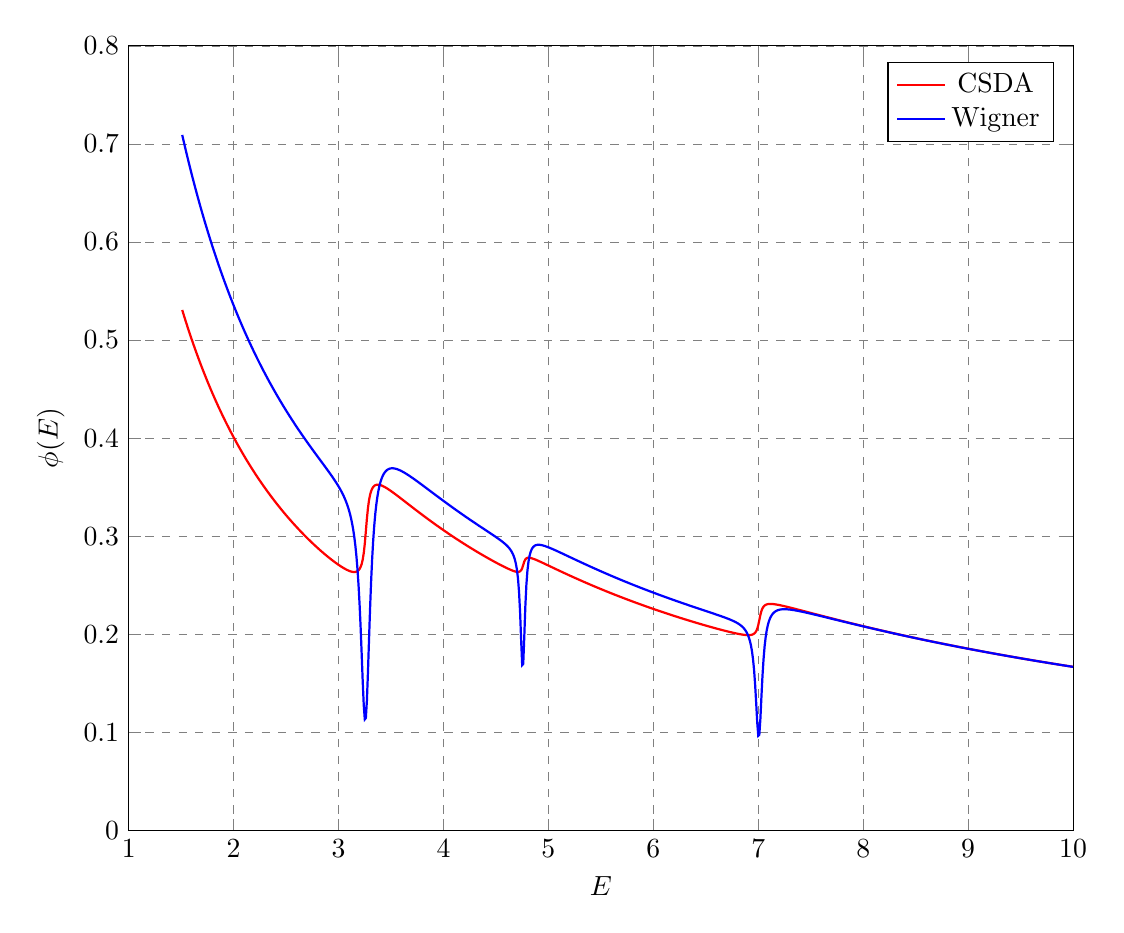
\begin{tikzpicture} \begin{axis}
[scale=1.75,
 xmin=1, xmax=10,
 ymin=0, ymax=0.8,
 grid=major, 
 major grid style={color=gray,line width=0.2pt, dashed},
 xlabel=$E$,
 ylabel=$\phi(E)$,
]

\addplot[line width=0.8pt, color=red] coordinates {
( 10.00 , 0.16675 ) ( 9.99 , 0.16692 ) ( 9.98 , 0.16708 ) ( 9.97 , 0.16725 ) ( 9.96 , 0.16742 ) ( 9.95 , 0.16759 ) ( 9.94 , 0.16775 ) ( 9.93 , 0.16792 ) ( 9.92 , 0.16809 ) ( 9.91 , 0.16826 ) ( 9.90 , 0.16843 ) ( 9.89 , 0.16860 ) ( 9.88 , 0.16877 ) ( 9.87 , 0.16894 ) ( 9.86 , 0.16911 ) ( 9.85 , 0.16928 ) ( 9.84 , 0.16946 ) ( 9.83 , 0.16963 ) ( 9.82 , 0.16980 ) ( 9.81 , 0.16997 ) ( 9.80 , 0.17015 ) ( 9.79 , 0.17032 ) ( 9.78 , 0.17049 ) ( 9.77 , 0.17067 ) ( 9.76 , 0.17084 ) ( 9.75 , 0.17102 ) ( 9.74 , 0.17119 ) ( 9.73 , 0.17137 ) ( 9.72 , 0.17154 ) ( 9.71 , 0.17172 ) ( 9.70 , 0.17190 ) ( 9.69 , 0.17207 ) ( 9.68 , 0.17225 ) ( 9.67 , 0.17243 ) ( 9.66 , 0.17261 ) ( 9.65 , 0.17279 ) ( 9.64 , 0.17296 ) ( 9.63 , 0.17314 ) ( 9.62 , 0.17332 ) ( 9.61 , 0.17350 ) ( 9.60 , 0.17368 ) ( 9.59 , 0.17386 ) ( 9.58 , 0.17405 ) ( 9.57 , 0.17423 ) ( 9.56 , 0.17441 ) ( 9.55 , 0.17459 ) ( 9.54 , 0.17477 ) ( 9.53 , 0.17496 ) ( 9.52 , 0.17514 ) ( 9.51 , 0.17532 ) ( 9.50 , 0.17551 ) ( 9.49 , 0.17569 ) ( 9.48 , 0.17588 ) ( 9.47 , 0.17606 ) ( 9.46 , 0.17625 ) ( 9.45 , 0.17643 ) ( 9.44 , 0.17662 ) ( 9.43 , 0.17681 ) ( 9.42 , 0.17699 ) ( 9.41 , 0.17718 ) ( 9.40 , 0.17737 ) ( 9.39 , 0.17756 ) ( 9.38 , 0.17775 ) ( 9.37 , 0.17794 ) ( 9.36 , 0.17813 ) ( 9.35 , 0.17832 ) ( 9.34 , 0.17851 ) ( 9.33 , 0.17870 ) ( 9.32 , 0.17889 ) ( 9.31 , 0.17908 ) ( 9.30 , 0.17927 ) ( 9.29 , 0.17946 ) ( 9.28 , 0.17966 ) ( 9.27 , 0.17985 ) ( 9.26 , 0.18004 ) ( 9.25 , 0.18024 ) ( 9.24 , 0.18043 ) ( 9.23 , 0.18063 ) ( 9.22 , 0.18082 ) ( 9.21 , 0.18102 ) ( 9.20 , 0.18121 ) ( 9.19 , 0.18141 ) ( 9.18 , 0.18161 ) ( 9.17 , 0.18181 ) ( 9.16 , 0.18200 ) ( 9.15 , 0.18220 ) ( 9.14 , 0.18240 ) ( 9.13 , 0.18260 ) ( 9.12 , 0.18280 ) ( 9.11 , 0.18300 ) ( 9.10 , 0.18320 ) ( 9.09 , 0.18340 ) ( 9.08 , 0.18360 ) ( 9.07 , 0.18380 ) ( 9.06 , 0.18401 ) ( 9.05 , 0.18421 ) ( 9.04 , 0.18441 ) ( 9.03 , 0.18461 ) ( 9.02 , 0.18482 ) ( 9.01 , 0.18502 ) ( 9.00 , 0.18523 ) ( 8.99 , 0.18543 ) ( 8.98 , 0.18564 ) ( 8.97 , 0.18584 ) ( 8.96 , 0.18605 ) ( 8.95 , 0.18626 ) ( 8.94 , 0.18647 ) ( 8.93 , 0.18667 ) ( 8.92 , 0.18688 ) ( 8.91 , 0.18709 ) ( 8.90 , 0.18730 ) ( 8.89 , 0.18751 ) ( 8.88 , 0.18772 ) ( 8.87 , 0.18793 ) ( 8.86 , 0.18814 ) ( 8.85 , 0.18835 ) ( 8.84 , 0.18857 ) ( 8.83 , 0.18878 ) ( 8.82 , 0.18899 ) ( 8.81 , 0.18921 ) ( 8.80 , 0.18942 ) ( 8.79 , 0.18963 ) ( 8.78 , 0.18985 ) ( 8.77 , 0.19007 ) ( 8.76 , 0.19028 ) ( 8.75 , 0.19050 ) ( 8.74 , 0.19071 ) ( 8.73 , 0.19093 ) ( 8.72 , 0.19115 ) ( 8.71 , 0.19137 ) ( 8.70 , 0.19159 ) ( 8.69 , 0.19181 ) ( 8.68 , 0.19203 ) ( 8.67 , 0.19225 ) ( 8.66 , 0.19247 ) ( 8.65 , 0.19269 ) ( 8.64 , 0.19291 ) ( 8.63 , 0.19313 ) ( 8.62 , 0.19336 ) ( 8.61 , 0.19358 ) ( 8.60 , 0.19380 ) ( 8.59 , 0.19403 ) ( 8.58 , 0.19425 ) ( 8.57 , 0.19448 ) ( 8.56 , 0.19470 ) ( 8.55 , 0.19493 ) ( 8.54 , 0.19516 ) ( 8.53 , 0.19538 ) ( 8.52 , 0.19561 ) ( 8.51 , 0.19584 ) ( 8.50 , 0.19607 ) ( 8.49 , 0.19630 ) ( 8.48 , 0.19653 ) ( 8.47 , 0.19676 ) ( 8.46 , 0.19699 ) ( 8.45 , 0.19722 ) ( 8.44 , 0.19745 ) ( 8.43 , 0.19769 ) ( 8.42 , 0.19792 ) ( 8.41 , 0.19815 ) ( 8.40 , 0.19839 ) ( 8.39 , 0.19862 ) ( 8.38 , 0.19886 ) ( 8.37 , 0.19909 ) ( 8.36 , 0.19933 ) ( 8.35 , 0.19957 ) ( 8.34 , 0.19980 ) ( 8.33 , 0.20004 ) ( 8.32 , 0.20028 ) ( 8.31 , 0.20052 ) ( 8.30 , 0.20076 ) ( 8.29 , 0.20100 ) ( 8.28 , 0.20124 ) ( 8.27 , 0.20148 ) ( 8.26 , 0.20172 ) ( 8.25 , 0.20197 ) ( 8.24 , 0.20221 ) ( 8.23 , 0.20245 ) ( 8.22 , 0.20270 ) ( 8.21 , 0.20294 ) ( 8.20 , 0.20319 ) ( 8.19 , 0.20343 ) ( 8.18 , 0.20368 ) ( 8.17 , 0.20393 ) ( 8.16 , 0.20417 ) ( 8.15 , 0.20442 ) ( 8.14 , 0.20467 ) ( 8.13 , 0.20492 ) ( 8.12 , 0.20517 ) ( 8.11 , 0.20542 ) ( 8.10 , 0.20567 ) ( 8.09 , 0.20592 ) ( 8.08 , 0.20617 ) ( 8.07 , 0.20642 ) ( 8.06 , 0.20668 ) ( 8.05 , 0.20693 ) ( 8.04 , 0.20719 ) ( 8.03 , 0.20744 ) ( 8.02 , 0.20770 ) ( 8.01 , 0.20795 ) ( 8.00 , 0.20821 ) ( 7.99 , 0.20846 ) ( 7.98 , 0.20872 ) ( 7.97 , 0.20898 ) ( 7.96 , 0.20924 ) ( 7.95 , 0.20950 ) ( 7.94 , 0.20976 ) ( 7.93 , 0.21002 ) ( 7.92 , 0.21028 ) ( 7.91 , 0.21054 ) ( 7.90 , 0.21080 ) ( 7.89 , 0.21107 ) ( 7.88 , 0.21133 ) ( 7.87 , 0.21159 ) ( 7.86 , 0.21186 ) ( 7.85 , 0.21212 ) ( 7.84 , 0.21239 ) ( 7.83 , 0.21266 ) ( 7.82 , 0.21292 ) ( 7.81 , 0.21319 ) ( 7.80 , 0.21346 ) ( 7.79 , 0.21373 ) ( 7.78 , 0.21399 ) ( 7.77 , 0.21426 ) ( 7.76 , 0.21453 ) ( 7.75 , 0.21480 ) ( 7.74 , 0.21507 ) ( 7.73 , 0.21535 ) ( 7.72 , 0.21562 ) ( 7.71 , 0.21589 ) ( 7.70 , 0.21616 ) ( 7.69 , 0.21644 ) ( 7.68 , 0.21671 ) ( 7.67 , 0.21699 ) ( 7.66 , 0.21726 ) ( 7.65 , 0.21754 ) ( 7.64 , 0.21781 ) ( 7.63 , 0.21809 ) ( 7.62 , 0.21837 ) ( 7.61 , 0.21864 ) ( 7.60 , 0.21892 ) ( 7.59 , 0.21920 ) ( 7.58 , 0.21948 ) ( 7.57 , 0.21976 ) ( 7.56 , 0.22003 ) ( 7.55 , 0.22031 ) ( 7.54 , 0.22059 ) ( 7.53 , 0.22087 ) ( 7.52 , 0.22115 ) ( 7.51 , 0.22143 ) ( 7.50 , 0.22171 ) ( 7.49 , 0.22199 ) ( 7.48 , 0.22227 ) ( 7.47 , 0.22256 ) ( 7.46 , 0.22284 ) ( 7.45 , 0.22312 ) ( 7.44 , 0.22340 ) ( 7.43 , 0.22368 ) ( 7.42 , 0.22396 ) ( 7.41 , 0.22424 ) ( 7.40 , 0.22452 ) ( 7.39 , 0.22480 ) ( 7.38 , 0.22507 ) ( 7.37 , 0.22535 ) ( 7.36 , 0.22563 ) ( 7.35 , 0.22591 ) ( 7.34 , 0.22618 ) ( 7.33 , 0.22645 ) ( 7.32 , 0.22673 ) ( 7.31 , 0.22700 ) ( 7.30 , 0.22726 ) ( 7.29 , 0.22753 ) ( 7.28 , 0.22779 ) ( 7.27 , 0.22805 ) ( 7.26 , 0.22831 ) ( 7.25 , 0.22856 ) ( 7.24 , 0.22881 ) ( 7.23 , 0.22905 ) ( 7.22 , 0.22929 ) ( 7.21 , 0.22952 ) ( 7.20 , 0.22974 ) ( 7.19 , 0.22995 ) ( 7.18 , 0.23015 ) ( 7.17 , 0.23033 ) ( 7.16 , 0.23050 ) ( 7.15 , 0.23065 ) ( 7.14 , 0.23077 ) ( 7.13 , 0.23086 ) ( 7.12 , 0.23090 ) ( 7.11 , 0.23090 ) ( 7.10 , 0.23083 ) ( 7.09 , 0.23067 ) ( 7.08 , 0.23038 ) ( 7.07 , 0.22992 ) ( 7.06 , 0.22920 ) ( 7.05 , 0.22809 ) ( 7.04 , 0.22637 ) ( 7.03 , 0.22369 ) ( 7.02 , 0.21967 ) ( 7.01 , 0.21441 ) ( 7.00 , 0.20928 ) ( 6.99 , 0.20551 ) ( 6.98 , 0.20307 ) ( 6.97 , 0.20153 ) ( 6.96 , 0.20055 ) ( 6.95 , 0.19992 ) ( 6.94 , 0.19952 ) ( 6.93 , 0.19927 ) ( 6.92 , 0.19913 ) ( 6.91 , 0.19907 ) ( 6.90 , 0.19907 ) ( 6.89 , 0.19912 ) ( 6.88 , 0.19920 ) ( 6.87 , 0.19932 ) ( 6.86 , 0.19945 ) ( 6.85 , 0.19960 ) ( 6.84 , 0.19978 ) ( 6.83 , 0.19996 ) ( 6.82 , 0.20015 ) ( 6.81 , 0.20036 ) ( 6.80 , 0.20058 ) ( 6.79 , 0.20080 ) ( 6.78 , 0.20103 ) ( 6.77 , 0.20126 ) ( 6.76 , 0.20150 ) ( 6.75 , 0.20175 ) ( 6.74 , 0.20200 ) ( 6.73 , 0.20225 ) ( 6.72 , 0.20251 ) ( 6.71 , 0.20277 ) ( 6.70 , 0.20304 ) ( 6.69 , 0.20331 ) ( 6.68 , 0.20358 ) ( 6.67 , 0.20385 ) ( 6.66 , 0.20413 ) ( 6.65 , 0.20441 ) ( 6.64 , 0.20469 ) ( 6.63 , 0.20497 ) ( 6.62 , 0.20526 ) ( 6.61 , 0.20554 ) ( 6.60 , 0.20583 ) ( 6.59 , 0.20612 ) ( 6.58 , 0.20642 ) ( 6.57 , 0.20671 ) ( 6.56 , 0.20701 ) ( 6.55 , 0.20731 ) ( 6.54 , 0.20761 ) ( 6.53 , 0.20791 ) ( 6.52 , 0.20821 ) ( 6.51 , 0.20852 ) ( 6.50 , 0.20882 ) ( 6.49 , 0.20913 ) ( 6.48 , 0.20944 ) ( 6.47 , 0.20975 ) ( 6.46 , 0.21006 ) ( 6.45 , 0.21037 ) ( 6.44 , 0.21069 ) ( 6.43 , 0.21100 ) ( 6.42 , 0.21132 ) ( 6.41 , 0.21164 ) ( 6.40 , 0.21196 ) ( 6.39 , 0.21228 ) ( 6.38 , 0.21260 ) ( 6.37 , 0.21293 ) ( 6.36 , 0.21325 ) ( 6.35 , 0.21358 ) ( 6.34 , 0.21391 ) ( 6.33 , 0.21423 ) ( 6.32 , 0.21456 ) ( 6.31 , 0.21490 ) ( 6.30 , 0.21523 ) ( 6.29 , 0.21556 ) ( 6.28 , 0.21590 ) ( 6.27 , 0.21623 ) ( 6.26 , 0.21657 ) ( 6.25 , 0.21691 ) ( 6.24 , 0.21725 ) ( 6.23 , 0.21759 ) ( 6.22 , 0.21793 ) ( 6.21 , 0.21828 ) ( 6.20 , 0.21862 ) ( 6.19 , 0.21897 ) ( 6.18 , 0.21932 ) ( 6.17 , 0.21967 ) ( 6.16 , 0.22002 ) ( 6.15 , 0.22037 ) ( 6.14 , 0.22072 ) ( 6.13 , 0.22107 ) ( 6.12 , 0.22143 ) ( 6.11 , 0.22178 ) ( 6.10 , 0.22214 ) ( 6.09 , 0.22250 ) ( 6.08 , 0.22286 ) ( 6.07 , 0.22322 ) ( 6.06 , 0.22358 ) ( 6.05 , 0.22395 ) ( 6.04 , 0.22431 ) ( 6.03 , 0.22468 ) ( 6.02 , 0.22505 ) ( 6.01 , 0.22542 ) ( 6.00 , 0.22579 ) ( 5.99 , 0.22616 ) ( 5.98 , 0.22653 ) ( 5.97 , 0.22691 ) ( 5.96 , 0.22728 ) ( 5.95 , 0.22766 ) ( 5.94 , 0.22804 ) ( 5.93 , 0.22841 ) ( 5.92 , 0.22880 ) ( 5.91 , 0.22918 ) ( 5.90 , 0.22956 ) ( 5.89 , 0.22995 ) ( 5.88 , 0.23033 ) ( 5.87 , 0.23072 ) ( 5.86 , 0.23111 ) ( 5.85 , 0.23150 ) ( 5.84 , 0.23189 ) ( 5.83 , 0.23228 ) ( 5.82 , 0.23268 ) ( 5.81 , 0.23307 ) ( 5.80 , 0.23347 ) ( 5.79 , 0.23387 ) ( 5.78 , 0.23427 ) ( 5.77 , 0.23467 ) ( 5.76 , 0.23507 ) ( 5.75 , 0.23547 ) ( 5.74 , 0.23588 ) ( 5.73 , 0.23629 ) ( 5.72 , 0.23669 ) ( 5.71 , 0.23710 ) ( 5.70 , 0.23752 ) ( 5.69 , 0.23793 ) ( 5.68 , 0.23834 ) ( 5.67 , 0.23876 ) ( 5.66 , 0.23917 ) ( 5.65 , 0.23959 ) ( 5.64 , 0.24001 ) ( 5.63 , 0.24043 ) ( 5.62 , 0.24086 ) ( 5.61 , 0.24128 ) ( 5.60 , 0.24171 ) ( 5.59 , 0.24213 ) ( 5.58 , 0.24256 ) ( 5.57 , 0.24299 ) ( 5.56 , 0.24342 ) ( 5.55 , 0.24386 ) ( 5.54 , 0.24429 ) ( 5.53 , 0.24473 ) ( 5.52 , 0.24516 ) ( 5.51 , 0.24560 ) ( 5.50 , 0.24604 ) ( 5.49 , 0.24649 ) ( 5.48 , 0.24693 ) ( 5.47 , 0.24738 ) ( 5.46 , 0.24782 ) ( 5.45 , 0.24827 ) ( 5.44 , 0.24872 ) ( 5.43 , 0.24917 ) ( 5.42 , 0.24963 ) ( 5.41 , 0.25008 ) ( 5.40 , 0.25054 ) ( 5.39 , 0.25100 ) ( 5.38 , 0.25146 ) ( 5.37 , 0.25192 ) ( 5.36 , 0.25238 ) ( 5.35 , 0.25284 ) ( 5.34 , 0.25331 ) ( 5.33 , 0.25378 ) ( 5.32 , 0.25425 ) ( 5.31 , 0.25472 ) ( 5.30 , 0.25519 ) ( 5.29 , 0.25566 ) ( 5.28 , 0.25614 ) ( 5.27 , 0.25662 ) ( 5.26 , 0.25709 ) ( 5.25 , 0.25758 ) ( 5.24 , 0.25806 ) ( 5.23 , 0.25854 ) ( 5.22 , 0.25903 ) ( 5.21 , 0.25951 ) ( 5.20 , 0.26000 ) ( 5.19 , 0.26049 ) ( 5.18 , 0.26098 ) ( 5.17 , 0.26147 ) ( 5.16 , 0.26197 ) ( 5.15 , 0.26246 ) ( 5.14 , 0.26296 ) ( 5.13 , 0.26346 ) ( 5.12 , 0.26395 ) ( 5.11 , 0.26446 ) ( 5.10 , 0.26496 ) ( 5.09 , 0.26546 ) ( 5.08 , 0.26596 ) ( 5.07 , 0.26647 ) ( 5.06 , 0.26697 ) ( 5.05 , 0.26748 ) ( 5.04 , 0.26799 ) ( 5.03 , 0.26850 ) ( 5.02 , 0.26900 ) ( 5.01 , 0.26951 ) ( 5.00 , 0.27002 ) ( 4.99 , 0.27053 ) ( 4.98 , 0.27103 ) ( 4.97 , 0.27154 ) ( 4.96 , 0.27204 ) ( 4.95 , 0.27255 ) ( 4.94 , 0.27305 ) ( 4.93 , 0.27354 ) ( 4.92 , 0.27403 ) ( 4.91 , 0.27452 ) ( 4.90 , 0.27500 ) ( 4.89 , 0.27546 ) ( 4.88 , 0.27592 ) ( 4.87 , 0.27635 ) ( 4.86 , 0.27677 ) ( 4.85 , 0.27715 ) ( 4.84 , 0.27750 ) ( 4.83 , 0.27778 ) ( 4.82 , 0.27798 ) ( 4.81 , 0.27805 ) ( 4.80 , 0.27791 ) ( 4.79 , 0.27742 ) ( 4.78 , 0.27631 ) ( 4.77 , 0.27413 ) ( 4.76 , 0.27070 ) ( 4.75 , 0.26730 ) ( 4.74 , 0.26519 ) ( 4.73 , 0.26412 ) ( 4.72 , 0.26366 ) ( 4.71 , 0.26353 ) ( 4.70 , 0.26360 ) ( 4.69 , 0.26380 ) ( 4.68 , 0.26408 ) ( 4.67 , 0.26443 ) ( 4.66 , 0.26481 ) ( 4.65 , 0.26523 ) ( 4.64 , 0.26567 ) ( 4.63 , 0.26613 ) ( 4.62 , 0.26661 ) ( 4.61 , 0.26711 ) ( 4.60 , 0.26761 ) ( 4.59 , 0.26813 ) ( 4.58 , 0.26865 ) ( 4.57 , 0.26919 ) ( 4.56 , 0.26973 ) ( 4.55 , 0.27027 ) ( 4.54 , 0.27082 ) ( 4.53 , 0.27138 ) ( 4.52 , 0.27195 ) ( 4.51 , 0.27251 ) ( 4.50 , 0.27309 ) ( 4.49 , 0.27366 ) ( 4.48 , 0.27424 ) ( 4.47 , 0.27483 ) ( 4.46 , 0.27542 ) ( 4.45 , 0.27601 ) ( 4.44 , 0.27661 ) ( 4.43 , 0.27721 ) ( 4.42 , 0.27781 ) ( 4.41 , 0.27842 ) ( 4.40 , 0.27903 ) ( 4.39 , 0.27964 ) ( 4.38 , 0.28026 ) ( 4.37 , 0.28088 ) ( 4.36 , 0.28151 ) ( 4.35 , 0.28213 ) ( 4.34 , 0.28276 ) ( 4.33 , 0.28340 ) ( 4.32 , 0.28403 ) ( 4.31 , 0.28468 ) ( 4.30 , 0.28532 ) ( 4.29 , 0.28597 ) ( 4.28 , 0.28662 ) ( 4.27 , 0.28727 ) ( 4.26 , 0.28792 ) ( 4.25 , 0.28858 ) ( 4.24 , 0.28925 ) ( 4.23 , 0.28991 ) ( 4.22 , 0.29058 ) ( 4.21 , 0.29125 ) ( 4.20 , 0.29193 ) ( 4.19 , 0.29261 ) ( 4.18 , 0.29329 ) ( 4.17 , 0.29397 ) ( 4.16 , 0.29466 ) ( 4.15 , 0.29535 ) ( 4.14 , 0.29605 ) ( 4.13 , 0.29675 ) ( 4.12 , 0.29745 ) ( 4.11 , 0.29815 ) ( 4.10 , 0.29886 ) ( 4.09 , 0.29957 ) ( 4.08 , 0.30028 ) ( 4.07 , 0.30100 ) ( 4.06 , 0.30172 ) ( 4.05 , 0.30244 ) ( 4.04 , 0.30317 ) ( 4.03 , 0.30390 ) ( 4.02 , 0.30463 ) ( 4.01 , 0.30537 ) ( 4.00 , 0.30611 ) ( 3.99 , 0.30685 ) ( 3.98 , 0.30760 ) ( 3.97 , 0.30835 ) ( 3.96 , 0.30910 ) ( 3.95 , 0.30985 ) ( 3.94 , 0.31061 ) ( 3.93 , 0.31137 ) ( 3.92 , 0.31214 ) ( 3.91 , 0.31291 ) ( 3.90 , 0.31368 ) ( 3.89 , 0.31445 ) ( 3.88 , 0.31523 ) ( 3.87 , 0.31601 ) ( 3.86 , 0.31679 ) ( 3.85 , 0.31758 ) ( 3.84 , 0.31837 ) ( 3.83 , 0.31916 ) ( 3.82 , 0.31996 ) ( 3.81 , 0.32076 ) ( 3.80 , 0.32156 ) ( 3.79 , 0.32236 ) ( 3.78 , 0.32317 ) ( 3.77 , 0.32398 ) ( 3.76 , 0.32479 ) ( 3.75 , 0.32560 ) ( 3.74 , 0.32642 ) ( 3.73 , 0.32723 ) ( 3.72 , 0.32805 ) ( 3.71 , 0.32887 ) ( 3.70 , 0.32970 ) ( 3.69 , 0.33052 ) ( 3.68 , 0.33135 ) ( 3.67 , 0.33217 ) ( 3.66 , 0.33300 ) ( 3.65 , 0.33383 ) ( 3.64 , 0.33466 ) ( 3.63 , 0.33549 ) ( 3.62 , 0.33631 ) ( 3.61 , 0.33714 ) ( 3.60 , 0.33797 ) ( 3.59 , 0.33879 ) ( 3.58 , 0.33961 ) ( 3.57 , 0.34042 ) ( 3.56 , 0.34124 ) ( 3.55 , 0.34204 ) ( 3.54 , 0.34284 ) ( 3.53 , 0.34363 ) ( 3.52 , 0.34442 ) ( 3.51 , 0.34519 ) ( 3.50 , 0.34595 ) ( 3.49 , 0.34669 ) ( 3.48 , 0.34742 ) ( 3.47 , 0.34813 ) ( 3.46 , 0.34881 ) ( 3.45 , 0.34946 ) ( 3.44 , 0.35007 ) ( 3.43 , 0.35064 ) ( 3.42 , 0.35117 ) ( 3.41 , 0.35163 ) ( 3.40 , 0.35201 ) ( 3.39 , 0.35230 ) ( 3.38 , 0.35248 ) ( 3.37 , 0.35251 ) ( 3.36 , 0.35236 ) ( 3.35 , 0.35197 ) ( 3.34 , 0.35126 ) ( 3.33 , 0.35011 ) ( 3.32 , 0.34838 ) ( 3.31 , 0.34581 ) ( 3.30 , 0.34203 ) ( 3.29 , 0.33651 ) ( 3.28 , 0.32857 ) ( 3.27 , 0.31773 ) ( 3.26 , 0.30482 ) ( 3.25 , 0.29241 ) ( 3.24 , 0.28273 ) ( 3.23 , 0.27600 ) ( 3.22 , 0.27151 ) ( 3.21 , 0.26852 ) ( 3.20 , 0.26652 ) ( 3.19 , 0.26519 ) ( 3.18 , 0.26432 ) ( 3.17 , 0.26380 ) ( 3.16 , 0.26352 ) ( 3.15 , 0.26343 ) ( 3.14 , 0.26348 ) ( 3.13 , 0.26365 ) ( 3.12 , 0.26391 ) ( 3.11 , 0.26425 ) ( 3.10 , 0.26466 ) ( 3.09 , 0.26511 ) ( 3.08 , 0.26562 ) ( 3.07 , 0.26616 ) ( 3.06 , 0.26674 ) ( 3.05 , 0.26735 ) ( 3.04 , 0.26799 ) ( 3.03 , 0.26865 ) ( 3.02 , 0.26933 ) ( 3.01 , 0.27004 ) ( 3.00 , 0.27076 ) ( 2.99 , 0.27150 ) ( 2.98 , 0.27226 ) ( 2.97 , 0.27303 ) ( 2.96 , 0.27382 ) ( 2.95 , 0.27462 ) ( 2.94 , 0.27544 ) ( 2.93 , 0.27627 ) ( 2.92 , 0.27711 ) ( 2.91 , 0.27796 ) ( 2.90 , 0.27882 ) ( 2.89 , 0.27970 ) ( 2.88 , 0.28058 ) ( 2.87 , 0.28148 ) ( 2.86 , 0.28238 ) ( 2.85 , 0.28330 ) ( 2.84 , 0.28422 ) ( 2.83 , 0.28516 ) ( 2.82 , 0.28610 ) ( 2.81 , 0.28706 ) ( 2.80 , 0.28802 ) ( 2.79 , 0.28900 ) ( 2.78 , 0.28998 ) ( 2.77 , 0.29097 ) ( 2.76 , 0.29197 ) ( 2.75 , 0.29299 ) ( 2.74 , 0.29401 ) ( 2.73 , 0.29504 ) ( 2.72 , 0.29608 ) ( 2.71 , 0.29712 ) ( 2.70 , 0.29818 ) ( 2.69 , 0.29925 ) ( 2.68 , 0.30033 ) ( 2.67 , 0.30141 ) ( 2.66 , 0.30251 ) ( 2.65 , 0.30361 ) ( 2.64 , 0.30473 ) ( 2.63 , 0.30585 ) ( 2.62 , 0.30698 ) ( 2.61 , 0.30813 ) ( 2.60 , 0.30928 ) ( 2.59 , 0.31044 ) ( 2.58 , 0.31162 ) ( 2.57 , 0.31280 ) ( 2.56 , 0.31399 ) ( 2.55 , 0.31520 ) ( 2.54 , 0.31641 ) ( 2.53 , 0.31763 ) ( 2.52 , 0.31887 ) ( 2.51 , 0.32011 ) ( 2.50 , 0.32137 ) ( 2.49 , 0.32263 ) ( 2.48 , 0.32391 ) ( 2.47 , 0.32520 ) ( 2.46 , 0.32650 ) ( 2.45 , 0.32781 ) ( 2.44 , 0.32913 ) ( 2.43 , 0.33046 ) ( 2.42 , 0.33181 ) ( 2.41 , 0.33316 ) ( 2.40 , 0.33453 ) ( 2.39 , 0.33591 ) ( 2.38 , 0.33730 ) ( 2.37 , 0.33871 ) ( 2.36 , 0.34013 ) ( 2.35 , 0.34155 ) ( 2.34 , 0.34300 ) ( 2.33 , 0.34445 ) ( 2.32 , 0.34592 ) ( 2.31 , 0.34740 ) ( 2.30 , 0.34889 ) ( 2.29 , 0.35040 ) ( 2.28 , 0.35192 ) ( 2.27 , 0.35346 ) ( 2.26 , 0.35501 ) ( 2.25 , 0.35657 ) ( 2.24 , 0.35815 ) ( 2.23 , 0.35974 ) ( 2.22 , 0.36134 ) ( 2.21 , 0.36296 ) ( 2.20 , 0.36460 ) ( 2.19 , 0.36625 ) ( 2.18 , 0.36792 ) ( 2.17 , 0.36960 ) ( 2.16 , 0.37130 ) ( 2.15 , 0.37301 ) ( 2.14 , 0.37475 ) ( 2.13 , 0.37649 ) ( 2.12 , 0.37826 ) ( 2.11 , 0.38004 ) ( 2.10 , 0.38184 ) ( 2.09 , 0.38365 ) ( 2.08 , 0.38549 ) ( 2.07 , 0.38734 ) ( 2.06 , 0.38921 ) ( 2.05 , 0.39109 ) ( 2.04 , 0.39300 ) ( 2.03 , 0.39493 ) ( 2.02 , 0.39687 ) ( 2.01 , 0.39884 ) ( 2.00 , 0.40082 ) ( 1.99 , 0.40283 ) ( 1.98 , 0.40485 ) ( 1.97 , 0.40690 ) ( 1.96 , 0.40897 ) ( 1.95 , 0.41106 ) ( 1.94 , 0.41317 ) ( 1.93 , 0.41530 ) ( 1.92 , 0.41745 ) ( 1.91 , 0.41963 ) ( 1.90 , 0.42183 ) ( 1.89 , 0.42406 ) ( 1.88 , 0.42631 ) ( 1.87 , 0.42858 ) ( 1.86 , 0.43088 ) ( 1.85 , 0.43320 ) ( 1.84 , 0.43555 ) ( 1.83 , 0.43792 ) ( 1.82 , 0.44032 ) ( 1.81 , 0.44275 ) ( 1.80 , 0.44520 ) ( 1.79 , 0.44768 ) ( 1.78 , 0.45019 ) ( 1.77 , 0.45273 ) ( 1.76 , 0.45530 ) ( 1.75 , 0.45789 ) ( 1.74 , 0.46052 ) ( 1.73 , 0.46318 ) ( 1.72 , 0.46586 ) ( 1.71 , 0.46859 ) ( 1.70 , 0.47134 ) ( 1.69 , 0.47412 ) ( 1.68 , 0.47694 ) ( 1.67 , 0.47979 ) ( 1.66 , 0.48268 ) ( 1.65 , 0.48560 ) ( 1.64 , 0.48856 ) ( 1.63 , 0.49155 ) ( 1.62 , 0.49459 ) ( 1.61 , 0.49766 ) ( 1.60 , 0.50076 ) ( 1.59 , 0.50391 ) ( 1.58 , 0.50710 ) ( 1.57 , 0.51033 ) ( 1.56 , 0.51360 ) ( 1.55 , 0.51691 ) ( 1.54 , 0.52027 ) ( 1.53 , 0.52367 ) ( 1.52 , 0.52711 ) ( 1.51 , 0.53060 ) 
};

\addplot[line width=0.8pt, color=blue] coordinates {
( 10.00 , 0.16673 ) ( 9.99 , 0.16690 ) ( 9.98 , 0.16706 ) ( 9.97 , 0.16723 ) ( 9.96 , 0.16740 ) ( 9.95 , 0.16757 ) ( 9.94 , 0.16774 ) ( 9.93 , 0.16790 ) ( 9.92 , 0.16807 ) ( 9.91 , 0.16824 ) ( 9.90 , 0.16841 ) ( 9.89 , 0.16858 ) ( 9.88 , 0.16875 ) ( 9.87 , 0.16892 ) ( 9.86 , 0.16909 ) ( 9.85 , 0.16926 ) ( 9.84 , 0.16944 ) ( 9.83 , 0.16961 ) ( 9.82 , 0.16978 ) ( 9.81 , 0.16995 ) ( 9.80 , 0.17012 ) ( 9.79 , 0.17030 ) ( 9.78 , 0.17047 ) ( 9.77 , 0.17065 ) ( 9.76 , 0.17082 ) ( 9.75 , 0.17099 ) ( 9.74 , 0.17117 ) ( 9.73 , 0.17135 ) ( 9.72 , 0.17152 ) ( 9.71 , 0.17170 ) ( 9.70 , 0.17187 ) ( 9.69 , 0.17205 ) ( 9.68 , 0.17223 ) ( 9.67 , 0.17241 ) ( 9.66 , 0.17258 ) ( 9.65 , 0.17276 ) ( 9.64 , 0.17294 ) ( 9.63 , 0.17312 ) ( 9.62 , 0.17330 ) ( 9.61 , 0.17348 ) ( 9.60 , 0.17366 ) ( 9.59 , 0.17384 ) ( 9.58 , 0.17402 ) ( 9.57 , 0.17420 ) ( 9.56 , 0.17438 ) ( 9.55 , 0.17456 ) ( 9.54 , 0.17475 ) ( 9.53 , 0.17493 ) ( 9.52 , 0.17511 ) ( 9.51 , 0.17530 ) ( 9.50 , 0.17548 ) ( 9.49 , 0.17566 ) ( 9.48 , 0.17585 ) ( 9.47 , 0.17603 ) ( 9.46 , 0.17622 ) ( 9.45 , 0.17641 ) ( 9.44 , 0.17659 ) ( 9.43 , 0.17678 ) ( 9.42 , 0.17696 ) ( 9.41 , 0.17715 ) ( 9.40 , 0.17734 ) ( 9.39 , 0.17753 ) ( 9.38 , 0.17772 ) ( 9.37 , 0.17791 ) ( 9.36 , 0.17809 ) ( 9.35 , 0.17828 ) ( 9.34 , 0.17847 ) ( 9.33 , 0.17867 ) ( 9.32 , 0.17886 ) ( 9.31 , 0.17905 ) ( 9.30 , 0.17924 ) ( 9.29 , 0.17943 ) ( 9.28 , 0.17962 ) ( 9.27 , 0.17982 ) ( 9.26 , 0.18001 ) ( 9.25 , 0.18020 ) ( 9.24 , 0.18040 ) ( 9.23 , 0.18059 ) ( 9.22 , 0.18079 ) ( 9.21 , 0.18098 ) ( 9.20 , 0.18118 ) ( 9.19 , 0.18138 ) ( 9.18 , 0.18157 ) ( 9.17 , 0.18177 ) ( 9.16 , 0.18197 ) ( 9.15 , 0.18216 ) ( 9.14 , 0.18236 ) ( 9.13 , 0.18256 ) ( 9.12 , 0.18276 ) ( 9.11 , 0.18296 ) ( 9.10 , 0.18316 ) ( 9.09 , 0.18336 ) ( 9.08 , 0.18356 ) ( 9.07 , 0.18376 ) ( 9.06 , 0.18396 ) ( 9.05 , 0.18417 ) ( 9.04 , 0.18437 ) ( 9.03 , 0.18457 ) ( 9.02 , 0.18478 ) ( 9.01 , 0.18498 ) ( 9.00 , 0.18518 ) ( 8.99 , 0.18539 ) ( 8.98 , 0.18559 ) ( 8.97 , 0.18580 ) ( 8.96 , 0.18601 ) ( 8.95 , 0.18621 ) ( 8.94 , 0.18642 ) ( 8.93 , 0.18663 ) ( 8.92 , 0.18684 ) ( 8.91 , 0.18704 ) ( 8.90 , 0.18725 ) ( 8.89 , 0.18746 ) ( 8.88 , 0.18767 ) ( 8.87 , 0.18788 ) ( 8.86 , 0.18809 ) ( 8.85 , 0.18830 ) ( 8.84 , 0.18852 ) ( 8.83 , 0.18873 ) ( 8.82 , 0.18894 ) ( 8.81 , 0.18915 ) ( 8.80 , 0.18937 ) ( 8.79 , 0.18958 ) ( 8.78 , 0.18979 ) ( 8.77 , 0.19001 ) ( 8.76 , 0.19022 ) ( 8.75 , 0.19044 ) ( 8.74 , 0.19066 ) ( 8.73 , 0.19087 ) ( 8.72 , 0.19109 ) ( 8.71 , 0.19131 ) ( 8.70 , 0.19153 ) ( 8.69 , 0.19174 ) ( 8.68 , 0.19196 ) ( 8.67 , 0.19218 ) ( 8.66 , 0.19240 ) ( 8.65 , 0.19262 ) ( 8.64 , 0.19285 ) ( 8.63 , 0.19307 ) ( 8.62 , 0.19329 ) ( 8.61 , 0.19351 ) ( 8.60 , 0.19373 ) ( 8.59 , 0.19396 ) ( 8.58 , 0.19418 ) ( 8.57 , 0.19441 ) ( 8.56 , 0.19463 ) ( 8.55 , 0.19486 ) ( 8.54 , 0.19508 ) ( 8.53 , 0.19531 ) ( 8.52 , 0.19554 ) ( 8.51 , 0.19576 ) ( 8.50 , 0.19599 ) ( 8.49 , 0.19622 ) ( 8.48 , 0.19645 ) ( 8.47 , 0.19668 ) ( 8.46 , 0.19691 ) ( 8.45 , 0.19714 ) ( 8.44 , 0.19737 ) ( 8.43 , 0.19760 ) ( 8.42 , 0.19783 ) ( 8.41 , 0.19806 ) ( 8.40 , 0.19830 ) ( 8.39 , 0.19853 ) ( 8.38 , 0.19876 ) ( 8.37 , 0.19900 ) ( 8.36 , 0.19923 ) ( 8.35 , 0.19947 ) ( 8.34 , 0.19971 ) ( 8.33 , 0.19994 ) ( 8.32 , 0.20018 ) ( 8.31 , 0.20042 ) ( 8.30 , 0.20065 ) ( 8.29 , 0.20089 ) ( 8.28 , 0.20113 ) ( 8.27 , 0.20137 ) ( 8.26 , 0.20161 ) ( 8.25 , 0.20185 ) ( 8.24 , 0.20209 ) ( 8.23 , 0.20233 ) ( 8.22 , 0.20258 ) ( 8.21 , 0.20282 ) ( 8.20 , 0.20306 ) ( 8.19 , 0.20331 ) ( 8.18 , 0.20355 ) ( 8.17 , 0.20379 ) ( 8.16 , 0.20404 ) ( 8.15 , 0.20428 ) ( 8.14 , 0.20453 ) ( 8.13 , 0.20478 ) ( 8.12 , 0.20502 ) ( 8.11 , 0.20527 ) ( 8.10 , 0.20552 ) ( 8.09 , 0.20577 ) ( 8.08 , 0.20602 ) ( 8.07 , 0.20627 ) ( 8.06 , 0.20652 ) ( 8.05 , 0.20677 ) ( 8.04 , 0.20702 ) ( 8.03 , 0.20727 ) ( 8.02 , 0.20752 ) ( 8.01 , 0.20777 ) ( 8.00 , 0.20803 ) ( 7.99 , 0.20828 ) ( 7.98 , 0.20853 ) ( 7.97 , 0.20879 ) ( 7.96 , 0.20904 ) ( 7.95 , 0.20930 ) ( 7.94 , 0.20955 ) ( 7.93 , 0.20981 ) ( 7.92 , 0.21007 ) ( 7.91 , 0.21032 ) ( 7.90 , 0.21058 ) ( 7.89 , 0.21084 ) ( 7.88 , 0.21110 ) ( 7.87 , 0.21135 ) ( 7.86 , 0.21161 ) ( 7.85 , 0.21187 ) ( 7.84 , 0.21213 ) ( 7.83 , 0.21239 ) ( 7.82 , 0.21265 ) ( 7.81 , 0.21291 ) ( 7.80 , 0.21317 ) ( 7.79 , 0.21343 ) ( 7.78 , 0.21369 ) ( 7.77 , 0.21396 ) ( 7.76 , 0.21422 ) ( 7.75 , 0.21448 ) ( 7.74 , 0.21474 ) ( 7.73 , 0.21500 ) ( 7.72 , 0.21526 ) ( 7.71 , 0.21553 ) ( 7.70 , 0.21579 ) ( 7.69 , 0.21605 ) ( 7.68 , 0.21631 ) ( 7.67 , 0.21658 ) ( 7.66 , 0.21684 ) ( 7.65 , 0.21710 ) ( 7.64 , 0.21736 ) ( 7.63 , 0.21762 ) ( 7.62 , 0.21788 ) ( 7.61 , 0.21815 ) ( 7.60 , 0.21841 ) ( 7.59 , 0.21867 ) ( 7.58 , 0.21892 ) ( 7.57 , 0.21918 ) ( 7.56 , 0.21944 ) ( 7.55 , 0.21970 ) ( 7.54 , 0.21995 ) ( 7.53 , 0.22021 ) ( 7.52 , 0.22046 ) ( 7.51 , 0.22072 ) ( 7.50 , 0.22097 ) ( 7.49 , 0.22121 ) ( 7.48 , 0.22146 ) ( 7.47 , 0.22171 ) ( 7.46 , 0.22195 ) ( 7.45 , 0.22219 ) ( 7.44 , 0.22243 ) ( 7.43 , 0.22266 ) ( 7.42 , 0.22289 ) ( 7.41 , 0.22312 ) ( 7.40 , 0.22334 ) ( 7.39 , 0.22355 ) ( 7.38 , 0.22376 ) ( 7.37 , 0.22397 ) ( 7.36 , 0.22417 ) ( 7.35 , 0.22436 ) ( 7.34 , 0.22454 ) ( 7.33 , 0.22471 ) ( 7.32 , 0.22487 ) ( 7.31 , 0.22501 ) ( 7.30 , 0.22514 ) ( 7.29 , 0.22526 ) ( 7.28 , 0.22535 ) ( 7.27 , 0.22543 ) ( 7.26 , 0.22548 ) ( 7.25 , 0.22550 ) ( 7.24 , 0.22548 ) ( 7.23 , 0.22543 ) ( 7.22 , 0.22532 ) ( 7.21 , 0.22517 ) ( 7.20 , 0.22494 ) ( 7.19 , 0.22464 ) ( 7.18 , 0.22423 ) ( 7.17 , 0.22371 ) ( 7.16 , 0.22304 ) ( 7.15 , 0.22219 ) ( 7.14 , 0.22110 ) ( 7.13 , 0.21971 ) ( 7.12 , 0.21794 ) ( 7.11 , 0.21565 ) ( 7.10 , 0.21268 ) ( 7.09 , 0.20878 ) ( 7.08 , 0.20359 ) ( 7.07 , 0.19662 ) ( 7.06 , 0.18716 ) ( 7.05 , 0.17431 ) ( 7.04 , 0.15722 ) ( 7.03 , 0.13592 ) ( 7.02 , 0.11340 ) ( 7.01 , 0.09742 ) ( 7.00 , 0.09643 ) ( 6.99 , 0.11015 ) ( 6.98 , 0.13000 ) ( 6.97 , 0.14865 ) ( 6.96 , 0.16348 ) ( 6.95 , 0.17455 ) ( 6.94 , 0.18269 ) ( 6.93 , 0.18873 ) ( 6.92 , 0.19328 ) ( 6.91 , 0.19678 ) ( 6.90 , 0.19953 ) ( 6.89 , 0.20174 ) ( 6.88 , 0.20354 ) ( 6.87 , 0.20505 ) ( 6.86 , 0.20633 ) ( 6.85 , 0.20743 ) ( 6.84 , 0.20840 ) ( 6.83 , 0.20926 ) ( 6.82 , 0.21003 ) ( 6.81 , 0.21074 ) ( 6.80 , 0.21139 ) ( 6.79 , 0.21199 ) ( 6.78 , 0.21255 ) ( 6.77 , 0.21309 ) ( 6.76 , 0.21359 ) ( 6.75 , 0.21408 ) ( 6.74 , 0.21454 ) ( 6.73 , 0.21499 ) ( 6.72 , 0.21543 ) ( 6.71 , 0.21585 ) ( 6.70 , 0.21626 ) ( 6.69 , 0.21667 ) ( 6.68 , 0.21707 ) ( 6.67 , 0.21746 ) ( 6.66 , 0.21785 ) ( 6.65 , 0.21823 ) ( 6.64 , 0.21861 ) ( 6.63 , 0.21898 ) ( 6.62 , 0.21935 ) ( 6.61 , 0.21972 ) ( 6.60 , 0.22009 ) ( 6.59 , 0.22045 ) ( 6.58 , 0.22081 ) ( 6.57 , 0.22118 ) ( 6.56 , 0.22154 ) ( 6.55 , 0.22190 ) ( 6.54 , 0.22225 ) ( 6.53 , 0.22261 ) ( 6.52 , 0.22297 ) ( 6.51 , 0.22333 ) ( 6.50 , 0.22369 ) ( 6.49 , 0.22404 ) ( 6.48 , 0.22440 ) ( 6.47 , 0.22476 ) ( 6.46 , 0.22511 ) ( 6.45 , 0.22547 ) ( 6.44 , 0.22583 ) ( 6.43 , 0.22619 ) ( 6.42 , 0.22655 ) ( 6.41 , 0.22691 ) ( 6.40 , 0.22727 ) ( 6.39 , 0.22763 ) ( 6.38 , 0.22799 ) ( 6.37 , 0.22835 ) ( 6.36 , 0.22872 ) ( 6.35 , 0.22908 ) ( 6.34 , 0.22944 ) ( 6.33 , 0.22981 ) ( 6.32 , 0.23017 ) ( 6.31 , 0.23054 ) ( 6.30 , 0.23091 ) ( 6.29 , 0.23128 ) ( 6.28 , 0.23165 ) ( 6.27 , 0.23202 ) ( 6.26 , 0.23239 ) ( 6.25 , 0.23276 ) ( 6.24 , 0.23313 ) ( 6.23 , 0.23351 ) ( 6.22 , 0.23388 ) ( 6.21 , 0.23426 ) ( 6.20 , 0.23464 ) ( 6.19 , 0.23502 ) ( 6.18 , 0.23540 ) ( 6.17 , 0.23578 ) ( 6.16 , 0.23616 ) ( 6.15 , 0.23654 ) ( 6.14 , 0.23693 ) ( 6.13 , 0.23731 ) ( 6.12 , 0.23770 ) ( 6.11 , 0.23808 ) ( 6.10 , 0.23847 ) ( 6.09 , 0.23886 ) ( 6.08 , 0.23925 ) ( 6.07 , 0.23964 ) ( 6.06 , 0.24004 ) ( 6.05 , 0.24043 ) ( 6.04 , 0.24083 ) ( 6.03 , 0.24123 ) ( 6.02 , 0.24162 ) ( 6.01 , 0.24202 ) ( 6.00 , 0.24242 ) ( 5.99 , 0.24282 ) ( 5.98 , 0.24323 ) ( 5.97 , 0.24363 ) ( 5.96 , 0.24404 ) ( 5.95 , 0.24445 ) ( 5.94 , 0.24485 ) ( 5.93 , 0.24526 ) ( 5.92 , 0.24567 ) ( 5.91 , 0.24609 ) ( 5.90 , 0.24650 ) ( 5.89 , 0.24691 ) ( 5.88 , 0.24733 ) ( 5.87 , 0.24775 ) ( 5.86 , 0.24817 ) ( 5.85 , 0.24859 ) ( 5.84 , 0.24901 ) ( 5.83 , 0.24943 ) ( 5.82 , 0.24986 ) ( 5.81 , 0.25028 ) ( 5.80 , 0.25071 ) ( 5.79 , 0.25114 ) ( 5.78 , 0.25157 ) ( 5.77 , 0.25200 ) ( 5.76 , 0.25243 ) ( 5.75 , 0.25286 ) ( 5.74 , 0.25330 ) ( 5.73 , 0.25374 ) ( 5.72 , 0.25417 ) ( 5.71 , 0.25461 ) ( 5.70 , 0.25505 ) ( 5.69 , 0.25550 ) ( 5.68 , 0.25594 ) ( 5.67 , 0.25639 ) ( 5.66 , 0.25683 ) ( 5.65 , 0.25728 ) ( 5.64 , 0.25773 ) ( 5.63 , 0.25818 ) ( 5.62 , 0.25863 ) ( 5.61 , 0.25909 ) ( 5.60 , 0.25954 ) ( 5.59 , 0.26000 ) ( 5.58 , 0.26046 ) ( 5.57 , 0.26092 ) ( 5.56 , 0.26138 ) ( 5.55 , 0.26184 ) ( 5.54 , 0.26231 ) ( 5.53 , 0.26277 ) ( 5.52 , 0.26324 ) ( 5.51 , 0.26371 ) ( 5.50 , 0.26418 ) ( 5.49 , 0.26465 ) ( 5.48 , 0.26512 ) ( 5.47 , 0.26560 ) ( 5.46 , 0.26607 ) ( 5.45 , 0.26655 ) ( 5.44 , 0.26703 ) ( 5.43 , 0.26751 ) ( 5.42 , 0.26799 ) ( 5.41 , 0.26847 ) ( 5.40 , 0.26896 ) ( 5.39 , 0.26944 ) ( 5.38 , 0.26993 ) ( 5.37 , 0.27042 ) ( 5.36 , 0.27091 ) ( 5.35 , 0.27140 ) ( 5.34 , 0.27189 ) ( 5.33 , 0.27239 ) ( 5.32 , 0.27288 ) ( 5.31 , 0.27338 ) ( 5.30 , 0.27387 ) ( 5.29 , 0.27437 ) ( 5.28 , 0.27487 ) ( 5.27 , 0.27537 ) ( 5.26 , 0.27587 ) ( 5.25 , 0.27637 ) ( 5.24 , 0.27687 ) ( 5.23 , 0.27738 ) ( 5.22 , 0.27788 ) ( 5.21 , 0.27839 ) ( 5.20 , 0.27889 ) ( 5.19 , 0.27939 ) ( 5.18 , 0.27990 ) ( 5.17 , 0.28040 ) ( 5.16 , 0.28091 ) ( 5.15 , 0.28141 ) ( 5.14 , 0.28191 ) ( 5.13 , 0.28242 ) ( 5.12 , 0.28292 ) ( 5.11 , 0.28341 ) ( 5.10 , 0.28391 ) ( 5.09 , 0.28441 ) ( 5.08 , 0.28490 ) ( 5.07 , 0.28538 ) ( 5.06 , 0.28587 ) ( 5.05 , 0.28634 ) ( 5.04 , 0.28681 ) ( 5.03 , 0.28728 ) ( 5.02 , 0.28773 ) ( 5.01 , 0.28817 ) ( 5.00 , 0.28860 ) ( 4.99 , 0.28902 ) ( 4.98 , 0.28941 ) ( 4.97 , 0.28979 ) ( 4.96 , 0.29014 ) ( 4.95 , 0.29045 ) ( 4.94 , 0.29073 ) ( 4.93 , 0.29096 ) ( 4.92 , 0.29112 ) ( 4.91 , 0.29122 ) ( 4.90 , 0.29121 ) ( 4.89 , 0.29108 ) ( 4.88 , 0.29079 ) ( 4.87 , 0.29028 ) ( 4.86 , 0.28948 ) ( 4.85 , 0.28826 ) ( 4.84 , 0.28647 ) ( 4.83 , 0.28382 ) ( 4.82 , 0.27988 ) ( 4.81 , 0.27394 ) ( 4.80 , 0.26477 ) ( 4.79 , 0.25042 ) ( 4.78 , 0.22825 ) ( 4.77 , 0.19765 ) ( 4.76 , 0.16973 ) ( 4.75 , 0.16857 ) ( 4.74 , 0.19405 ) ( 4.73 , 0.22245 ) ( 4.72 , 0.24316 ) ( 4.71 , 0.25677 ) ( 4.70 , 0.26575 ) ( 4.69 , 0.27187 ) ( 4.68 , 0.27625 ) ( 4.67 , 0.27951 ) ( 4.66 , 0.28205 ) ( 4.65 , 0.28410 ) ( 4.64 , 0.28580 ) ( 4.63 , 0.28727 ) ( 4.62 , 0.28856 ) ( 4.61 , 0.28972 ) ( 4.60 , 0.29078 ) ( 4.59 , 0.29177 ) ( 4.58 , 0.29270 ) ( 4.57 , 0.29358 ) ( 4.56 , 0.29443 ) ( 4.55 , 0.29525 ) ( 4.54 , 0.29605 ) ( 4.53 , 0.29682 ) ( 4.52 , 0.29758 ) ( 4.51 , 0.29834 ) ( 4.50 , 0.29908 ) ( 4.49 , 0.29981 ) ( 4.48 , 0.30053 ) ( 4.47 , 0.30126 ) ( 4.46 , 0.30197 ) ( 4.45 , 0.30269 ) ( 4.44 , 0.30340 ) ( 4.43 , 0.30411 ) ( 4.42 , 0.30482 ) ( 4.41 , 0.30553 ) ( 4.40 , 0.30623 ) ( 4.39 , 0.30694 ) ( 4.38 , 0.30765 ) ( 4.37 , 0.30836 ) ( 4.36 , 0.30907 ) ( 4.35 , 0.30978 ) ( 4.34 , 0.31049 ) ( 4.33 , 0.31121 ) ( 4.32 , 0.31192 ) ( 4.31 , 0.31264 ) ( 4.30 , 0.31336 ) ( 4.29 , 0.31408 ) ( 4.28 , 0.31480 ) ( 4.27 , 0.31553 ) ( 4.26 , 0.31625 ) ( 4.25 , 0.31698 ) ( 4.24 , 0.31771 ) ( 4.23 , 0.31845 ) ( 4.22 , 0.31918 ) ( 4.21 , 0.31992 ) ( 4.20 , 0.32066 ) ( 4.19 , 0.32140 ) ( 4.18 , 0.32215 ) ( 4.17 , 0.32289 ) ( 4.16 , 0.32364 ) ( 4.15 , 0.32440 ) ( 4.14 , 0.32515 ) ( 4.13 , 0.32591 ) ( 4.12 , 0.32667 ) ( 4.11 , 0.32743 ) ( 4.10 , 0.32819 ) ( 4.09 , 0.32896 ) ( 4.08 , 0.32973 ) ( 4.07 , 0.33050 ) ( 4.06 , 0.33127 ) ( 4.05 , 0.33205 ) ( 4.04 , 0.33283 ) ( 4.03 , 0.33361 ) ( 4.02 , 0.33439 ) ( 4.01 , 0.33517 ) ( 4.00 , 0.33596 ) ( 3.99 , 0.33675 ) ( 3.98 , 0.33754 ) ( 3.97 , 0.33833 ) ( 3.96 , 0.33912 ) ( 3.95 , 0.33992 ) ( 3.94 , 0.34072 ) ( 3.93 , 0.34151 ) ( 3.92 , 0.34231 ) ( 3.91 , 0.34311 ) ( 3.90 , 0.34391 ) ( 3.89 , 0.34472 ) ( 3.88 , 0.34552 ) ( 3.87 , 0.34632 ) ( 3.86 , 0.34712 ) ( 3.85 , 0.34793 ) ( 3.84 , 0.34873 ) ( 3.83 , 0.34953 ) ( 3.82 , 0.35033 ) ( 3.81 , 0.35113 ) ( 3.80 , 0.35193 ) ( 3.79 , 0.35272 ) ( 3.78 , 0.35351 ) ( 3.77 , 0.35430 ) ( 3.76 , 0.35509 ) ( 3.75 , 0.35587 ) ( 3.74 , 0.35665 ) ( 3.73 , 0.35742 ) ( 3.72 , 0.35818 ) ( 3.71 , 0.35893 ) ( 3.70 , 0.35968 ) ( 3.69 , 0.36042 ) ( 3.68 , 0.36114 ) ( 3.67 , 0.36186 ) ( 3.66 , 0.36256 ) ( 3.65 , 0.36324 ) ( 3.64 , 0.36390 ) ( 3.63 , 0.36455 ) ( 3.62 , 0.36517 ) ( 3.61 , 0.36576 ) ( 3.60 , 0.36633 ) ( 3.59 , 0.36686 ) ( 3.58 , 0.36736 ) ( 3.57 , 0.36781 ) ( 3.56 , 0.36821 ) ( 3.55 , 0.36856 ) ( 3.54 , 0.36884 ) ( 3.53 , 0.36905 ) ( 3.52 , 0.36918 ) ( 3.51 , 0.36921 ) ( 3.50 , 0.36913 ) ( 3.49 , 0.36892 ) ( 3.48 , 0.36856 ) ( 3.47 , 0.36802 ) ( 3.46 , 0.36727 ) ( 3.45 , 0.36627 ) ( 3.44 , 0.36498 ) ( 3.43 , 0.36333 ) ( 3.42 , 0.36126 ) ( 3.41 , 0.35866 ) ( 3.40 , 0.35543 ) ( 3.39 , 0.35142 ) ( 3.38 , 0.34642 ) ( 3.37 , 0.34021 ) ( 3.36 , 0.33247 ) ( 3.35 , 0.32278 ) ( 3.34 , 0.31066 ) ( 3.33 , 0.29549 ) ( 3.32 , 0.27658 ) ( 3.31 , 0.25332 ) ( 3.30 , 0.22545 ) ( 3.29 , 0.19372 ) ( 3.28 , 0.16085 ) ( 3.27 , 0.13214 ) ( 3.26 , 0.11458 ) ( 3.25 , 0.11324 ) ( 3.24 , 0.12769 ) ( 3.23 , 0.15238 ) ( 3.22 , 0.18060 ) ( 3.21 , 0.20759 ) ( 3.20 , 0.23114 ) ( 3.19 , 0.25076 ) ( 3.18 , 0.26678 ) ( 3.17 , 0.27979 ) ( 3.16 , 0.29039 ) ( 3.15 , 0.29911 ) ( 3.14 , 0.30636 ) ( 3.13 , 0.31247 ) ( 3.12 , 0.31768 ) ( 3.11 , 0.32218 ) ( 3.10 , 0.32612 ) ( 3.09 , 0.32961 ) ( 3.08 , 0.33274 ) ( 3.07 , 0.33558 ) ( 3.06 , 0.33818 ) ( 3.05 , 0.34059 ) ( 3.04 , 0.34284 ) ( 3.03 , 0.34495 ) ( 3.02 , 0.34695 ) ( 3.01 , 0.34886 ) ( 3.00 , 0.35069 ) ( 2.99 , 0.35245 ) ( 2.98 , 0.35416 ) ( 2.97 , 0.35582 ) ( 2.96 , 0.35744 ) ( 2.95 , 0.35903 ) ( 2.94 , 0.36059 ) ( 2.93 , 0.36212 ) ( 2.92 , 0.36364 ) ( 2.91 , 0.36514 ) ( 2.90 , 0.36663 ) ( 2.89 , 0.36810 ) ( 2.88 , 0.36957 ) ( 2.87 , 0.37103 ) ( 2.86 , 0.37249 ) ( 2.85 , 0.37394 ) ( 2.84 , 0.37539 ) ( 2.83 , 0.37684 ) ( 2.82 , 0.37828 ) ( 2.81 , 0.37973 ) ( 2.80 , 0.38119 ) ( 2.79 , 0.38264 ) ( 2.78 , 0.38410 ) ( 2.77 , 0.38556 ) ( 2.76 , 0.38703 ) ( 2.75 , 0.38850 ) ( 2.74 , 0.38998 ) ( 2.73 , 0.39146 ) ( 2.72 , 0.39296 ) ( 2.71 , 0.39445 ) ( 2.70 , 0.39596 ) ( 2.69 , 0.39747 ) ( 2.68 , 0.39900 ) ( 2.67 , 0.40053 ) ( 2.66 , 0.40207 ) ( 2.65 , 0.40361 ) ( 2.64 , 0.40517 ) ( 2.63 , 0.40674 ) ( 2.62 , 0.40832 ) ( 2.61 , 0.40991 ) ( 2.60 , 0.41151 ) ( 2.59 , 0.41312 ) ( 2.58 , 0.41474 ) ( 2.57 , 0.41637 ) ( 2.56 , 0.41801 ) ( 2.55 , 0.41967 ) ( 2.54 , 0.42133 ) ( 2.53 , 0.42301 ) ( 2.52 , 0.42470 ) ( 2.51 , 0.42641 ) ( 2.50 , 0.42812 ) ( 2.49 , 0.42985 ) ( 2.48 , 0.43160 ) ( 2.47 , 0.43335 ) ( 2.46 , 0.43512 ) ( 2.45 , 0.43691 ) ( 2.44 , 0.43870 ) ( 2.43 , 0.44052 ) ( 2.42 , 0.44234 ) ( 2.41 , 0.44418 ) ( 2.40 , 0.44604 ) ( 2.39 , 0.44791 ) ( 2.38 , 0.44980 ) ( 2.37 , 0.45170 ) ( 2.36 , 0.45362 ) ( 2.35 , 0.45555 ) ( 2.34 , 0.45750 ) ( 2.33 , 0.45947 ) ( 2.32 , 0.46145 ) ( 2.31 , 0.46345 ) ( 2.30 , 0.46547 ) ( 2.29 , 0.46750 ) ( 2.28 , 0.46955 ) ( 2.27 , 0.47162 ) ( 2.26 , 0.47371 ) ( 2.25 , 0.47582 ) ( 2.24 , 0.47794 ) ( 2.23 , 0.48009 ) ( 2.22 , 0.48225 ) ( 2.21 , 0.48444 ) ( 2.20 , 0.48664 ) ( 2.19 , 0.48886 ) ( 2.18 , 0.49110 ) ( 2.17 , 0.49337 ) ( 2.16 , 0.49565 ) ( 2.15 , 0.49796 ) ( 2.14 , 0.50028 ) ( 2.13 , 0.50263 ) ( 2.12 , 0.50500 ) ( 2.11 , 0.50740 ) ( 2.10 , 0.50981 ) ( 2.09 , 0.51225 ) ( 2.08 , 0.51471 ) ( 2.07 , 0.51720 ) ( 2.06 , 0.51971 ) ( 2.05 , 0.52225 ) ( 2.04 , 0.52481 ) ( 2.03 , 0.52739 ) ( 2.02 , 0.53000 ) ( 2.01 , 0.53264 ) ( 2.00 , 0.53530 ) ( 1.99 , 0.53799 ) ( 1.98 , 0.54071 ) ( 1.97 , 0.54345 ) ( 1.96 , 0.54622 ) ( 1.95 , 0.54903 ) ( 1.94 , 0.55186 ) ( 1.93 , 0.55472 ) ( 1.92 , 0.55760 ) ( 1.91 , 0.56052 ) ( 1.90 , 0.56347 ) ( 1.89 , 0.56646 ) ( 1.88 , 0.56947 ) ( 1.87 , 0.57252 ) ( 1.86 , 0.57559 ) ( 1.85 , 0.57871 ) ( 1.84 , 0.58185 ) ( 1.83 , 0.58503 ) ( 1.82 , 0.58825 ) ( 1.81 , 0.59150 ) ( 1.80 , 0.59478 ) ( 1.79 , 0.59811 ) ( 1.78 , 0.60147 ) ( 1.77 , 0.60487 ) ( 1.76 , 0.60831 ) ( 1.75 , 0.61179 ) ( 1.74 , 0.61530 ) ( 1.73 , 0.61886 ) ( 1.72 , 0.62246 ) ( 1.71 , 0.62610 ) ( 1.70 , 0.62979 ) ( 1.69 , 0.63352 ) ( 1.68 , 0.63729 ) ( 1.67 , 0.64111 ) ( 1.66 , 0.64497 ) ( 1.65 , 0.64889 ) ( 1.64 , 0.65285 ) ( 1.63 , 0.65685 ) ( 1.62 , 0.66091 ) ( 1.61 , 0.66502 ) ( 1.60 , 0.66918 ) ( 1.59 , 0.67339 ) ( 1.58 , 0.67766 ) ( 1.57 , 0.68198 ) ( 1.56 , 0.68636 ) ( 1.55 , 0.69079 ) ( 1.54 , 0.69528 ) ( 1.53 , 0.69983 ) ( 1.52 , 0.70444 ) ( 1.51 , 0.70911 ) 
};

\legend{CSDA,Wigner}
\end{axis}
\end{tikzpicture}
\caption{Comparison of the scalar flux spectra predicted by the continuous slowing down and Wigner synthetic kernel approximations.}
 \label{Fig:thermalization_fluxSpectraComparision}
\end{center}
\end{figure}

One might wonder if we can do even better by keeping more terms in the Taylor series expansion. Indeed we can, and it is common to use a second-order expansion in what is called the Grueling-Goertzel approximation. This is more accurate and is particularly useful for scattering off deuterium in heavy water moderated systems. However, since light water is the most common moderator, and the Wigner synthetic scattering kernel reduces to the exact result in this case and is very accurate for heavy nuclides we may encounter, the first-order Taylor expansion is often good enough for a large class of practical reactor analyses.

%%%%%%%%%%%%%%%%%%%%%%%%%%%%%%%%%%%%%%%%%%%%%%%%%%%%%%%%%%%%%%%%%%%%%%%%%%%%%%%%%%%%%%%%%%%%%%%%%%%%
\section{Resonance Treatments}

In the previous section, we developed a theory for the slowing down of neutrons and the calculation of the scalar flux spectra. The first model is the continuous slowing down or Fermi age approximation, which is reasonable for predicting leakage but fails to treat resonances properly. The second model used a first-order Taylor expansion to construct the Wigner synthetic scattering kernel that addressed many of the problems, but we had to make an assumption of either a single isotope or a constant scattering cross section in a homogenized mixture. The former is a contrived case and the latter is rather dubious because the scattering cross section varies around the resonances. 

In this section, we develop approximate models for treating resonances with realistic cross sections that are surprisingly accurate and quite usable for most scenarios encountered in the slowing down region. This analysis is specific to the case of a homogeneous mixture. While this is a good start, it is unfortunately not quite good enough for analyzing actual reactors because the fuel-moderator heterogeneity has a significant impact on the resonance integrals. However, the techniques we develop in this section are used for this more complicated case, so we discuss them first.

\subsection{Resonance Integrals}

The absorptivity of a resonance can be characterized by the resonance integral, which depends upon the microscopic absorption cross section $\sigma_a(E)$ and the local flux spectrum within the resonance $\phi(E)$. We define the resonance integral for the $j$th resonance as
\begin{align}
  I_j = \int_{\Delta E_{rj}} \sigma_a(E) \phi(E) dE .
\end{align}
Here $\phi(E)$ is normalized such that $\phi(E_0) = 1/E_0$. $\Delta E_{rj}$ is the effective or practical width of the resonance and now we leave this ambiguous, but will return to this topic once we develop the model further.

Recall the point of this chapter is to provide information to compute the multigroup cross sections. Given some usually reasonable approximations, we can directly relate the multigroup cross section to the sum of resonance integrals within the energy group. Here we assume:
\begin{enumerate}
  \item Absorption is insignificant in the slowing down range except within the resonances. This tends to be reasonable because the absorption cross section outside resonances goes as $C/v$ and the coefficient $C$ is usually sufficiently small such that the cross section is comparatively quite small.
  \item The resonances are isolated. This means they do not meaningfully overlap in energy space such that the resonance integral for one resonance does not impact another. This occurs because a resonance by itself will cause a dip in the flux spectrum that influences the amount of absorption. If we have two or more overlapping resonances in the same energy range, the dip in the flux spectrum needs to account for both of them.
  \item The energy group is sufficiently wide and the resonances are both (a) sufficiently narrow, and (b) not too absorbent such that most of the energy spectrum within the group can be described with $1/E$ behavior.
\end{enumerate}

With these in mind, we write down the definition of the multigroup absorption cross section assuming a single isotope:
\begin{align}
  \Sigma_{a,g} = \dfrac{ \displaystyle\int_g N \sigma_a(E) \phi(E) dE }{ \displaystyle\int_g \phi(E) dE } .
\end{align}
By the first assumption, we can write the integral in the numerator of the absorption density as the sum of the integrals over the absorption densities for each resonance $j$ within the group $g$ as
\begin{align}
  \Sigma_{a,g} = \dfrac{ \displaystyle\sum_{j \in g} \int_{\Delta E_{rj}} N \sigma_a(E) \phi(E) dE }{ \displaystyle\int_g \phi(E) dE } .
\end{align}
By the second assumption that all resonances are separated and non-interacting, we can write those integrals as the sum of the resonance integrals,
\begin{align}
  \Sigma_{a,g} = \dfrac{ N \displaystyle\sum_{j \in g} I_j }{ \displaystyle\int_g \phi(E) dE } .
\end{align}
By the third assumption that a majority of the group is described by a $1/E$ spectrum, we can approximate the denominator as the width of the group in lethargy space,
\begin{align}
   \int_g \phi(E) dE \approx \int_g \frac{dE}{E} = \ln\left( \frac{E_{g}}{E_{g-1}} \right) = \Delta u_g .
\end{align}
In reality we know that the the flux spectrum is reduced slightly after each resonance. This would be a source of error, but note that this reduction also occurs when computing the resonance integrals in the numerator as well. The effect of this reduction in both the numerator and denominator is such that the errors incurred mostly cancel out.

Therefore, the group absorption cross section is
\begin{align}
  \Sigma_{a,g} = \frac{N}{\Delta u_g} \displaystyle\sum_{j \in g} I_j .
\end{align}
This means to compute the resonance integrals, which again require finding the scalar flux spectra within the group. 

\subsection{Moderator-Resonance Absorber Mixture Model}

For this analysis, we assume a mixture of two species: a moderator and a resonance absorber. We further assume the reactor is very large such that we can neglect leakage entirely, setting $B^2 = 0$. Given this, we can write down the neutron balance relationship for the mixture in the slowing down range:
\begin{align}
  \Sigma_t(E) \phi(E) = \int_E^{E/\alpha^M} \frac{\Sigma_s^M(E')}{ 1 - \alpha^M } \phi(E') \frac{dE'}{E'} + \int_E^{E/\alpha^R} \frac{\Sigma_s^R(E')}{ 1 - \alpha^R } \phi(E') \frac{dE'}{E'} .
\end{align}
Here we denote the superscript $M$ to be for the moderator and $R$ to be for the resonance absorber. Quantities without a superscript are for the entire mixture.

The moderator is assumed to consist of light nuclei (else they would not be an effective moderator) with a constant potential cross section and negligible absorption in the thermal energy range. We describe the cross sections as
\begin{subequations}
\begin{align}
  \Sigma_s^M(E) &= \Sigma_s^M, \\*
  \Sigma_a^M(E) &= 0.
\end{align}
\end{subequations}

The resonance absorber may either be light or heavy and has isolated resonances. The absorption cross section is negligible outside the resonances and typically large within them. The scattering cross section is described as constant potential scattering outside the resonances and having a resonance scattering cross section consisting of compound nucleus formation and interference terms. We describe these as
\begin{subequations}
\begin{align}
  \Sigma_s^R(E) &= \left\{ \begin{array}{l l}
  \Sigma_p^R,					& \quad \text{outside resonances,} \\
  \Sigma_p^R + \Sigma_{rs}^R(E), & \quad \text{within resonances,}  \\ \end{array} \right.
\end{align}
\begin{align}
  \Sigma_a^R(E) &= \left\{ \begin{array}{l l}
  0,			 & \quad \text{outside resonances,} \\
  \Sigma_a^R(E), & \quad \text{within resonances.}  \\ \end{array} \right.
\end{align}
\end{subequations}

For either the moderator or the resonance absorber, we can define the scattering range, which is the maximum amount of energy that a neutron can lose in a single collision with either the moderator or resonance absorpber and reach an energy $E$:
\begin{align}
  \Delta E_s = \frac{E'}{\alpha} - E'  = \left( \frac{ 1 - \alpha }{ \alpha } \right) E' .
\end{align}
This scattering parameters $\alpha$ can be taken to be with respect to either nuclide. We use this scattering range to assess the applicability of various models. Note that this is not the only choice used. Often one uses the average energy transfer as opposed to the full range.

\subsection{Narrow Resonance (NR) Approximation} \label{Sec:thermalization_narrowResonanceApproximation_HomogeneousMixture}

The first model assumes a resonance is narrow with respect to the scattering ranges of \emph{both} the moderator and resonance absorber. For moderators this is essentially always the case because they consist of light nuclides. It turns out that for most resonances this is quite accurate, especially for the ones that are higher in energy. We call this the narrow resonance or NR approximation for short. The NR approximation is valid when
\begin{align}
  \frac{ \Delta E_s^R }{ \Delta E_{rj} } \gg 1 .
\end{align}

When this is true, the energy spectrum is well described by $1/E$ over most of the scattering ranges of both the moderator and resonance absorber. Therefore, the spectra within scattering integrals are mostly $1/E$ and the effect of the dips within the resonances will not contribute significantly and can be approximated by just assuming that spectrum over the entire range. Furthermore, the resonance absorber scattering cross section is mostly constant over the range of integration. Therefore, the neutron balance relationship becomes
\begin{align}
  \Sigma_t(E) \phi_{NR}(E) = \int_E^{E/\alpha^M} \frac{\Sigma_s^M}{ 1 - \alpha^M } \frac{1}{E'} \frac{dE'}{E'} + \int_E^{E/\alpha^R} \frac{\Sigma_p^R}{ 1 - \alpha^R } \frac{1}{E'} \frac{dE'}{E'} .
\end{align}
Here we denote the scalar flux with a $NR$ subscript to delineate it from other approximations. Note that the right-hand side no longer involves any unknown scalar flux. Therefore, we can directly evaluate the integrals and solve for $\phi_{NR}(E)$. This is
\begin{align}
  \phi_{NR}(E) = \frac{1}{E} \left[ \frac{ \Sigma_s^M + \Sigma_p^R }{ \Sigma_s^M + \Sigma_s^R(E) + \Sigma_a^R(E) } \right] . \label{Eq:thermalization_NR_FluxSpectrum}
\end{align}

\subsection{Narrow Resonance, Infinite Mass (NRIM) Approximation}

The second model assumes the resonance is narrow with respect to the scattering width of the moderator, but wide with respect to that for the resonance absorber. We call this the narrow resonance, infinite mass (NRIM) approximation or sometimes the wide resonance approximation. This occurs when
\begin{align}
  \frac{ \Delta E_s^R }{ \Delta E_{rj} } \ll 1 .
\end{align}
This implies that the amount of energy lost for a neutron scattering off the resonance absorber is effectively infinite with \emph{respect to that resonance}. 

Since the moderator is narrow, the analysis we did before of replacing the flux spectrum in the scattering integral with $1/E$ is still valid. For the scattering integral of the resonance absorber, we take the limit as $\alpha^R$ approaches one from the left:
\begin{align}
  \lim_{\alpha^R \rightarrow 1^-} \int_E^{E/\alpha^R} \frac{\Sigma_s^R(E)}{ 1 - \alpha^R } \phi(E') \frac{dE'}{E'} 
  = \dfrac{ \displaystyle\lim_{\alpha^R \rightarrow 1^-} \int_E^{E/\alpha^R} \Sigma_s^R(E) \phi(E') \dfrac{dE'}{E'} }{ \displaystyle\lim_{\alpha^R \rightarrow 1^-} 1 - \alpha^R } = \frac{0}{0} . \nonumber
\end{align}
Getting $0/0$ motivates us to try L'Hopital's rule by taking the derivative of the numerator and denominator with respect to $\alpha^R$. To do this, we need to use the Leibniz rule to differentiate the numerator. Trying this again, we get
\begin{align}
  &\lim_{\alpha^R \rightarrow 1^-} \int_E^{E/\alpha^R} \frac{\Sigma_s^R(E)}{ 1 - \alpha^R } \phi(E') \frac{dE'}{E'} \nonumber \\
  &= \dfrac{ \displaystyle\lim_{\alpha^R \rightarrow 1^-} \int_E^{E/\alpha^R} \Sigma_s^R(E') \phi(E') \dfrac{dE'}{E'} }{ \displaystyle\lim_{\alpha^R \rightarrow 1^-} 1 - \alpha^R }  \nonumber \\
  &= \dfrac{ \displaystyle\lim_{\alpha^R \rightarrow 1^-}  \Sigma_s^R(E'/\alpha^R) \frac{\phi(E/\alpha^R)}{(E/\alpha^R)} \frac{d}{d\alpha^R} \left( \frac{E}{\alpha^R} \right)  }{ \displaystyle\lim_{\alpha^R \rightarrow 1^-} (-1) } \nonumber \\
  &= - \displaystyle\lim_{\alpha^R \rightarrow 1^-}  \Sigma_s^R(E'/\alpha^R) \frac{\phi(E/\alpha^R)}{(E/\alpha^R)} \left( -\frac{E}{( \alpha^R )^2} \right) \nonumber \\
  &= \Sigma_s^R(E) \phi(E) .
\end{align}

Inserting this into the neutron balance relationship gives
\begin{align}
  \Sigma_t(E) \phi_{NRIM}(E) = \int_E^{E/\alpha^M} \frac{\Sigma_s^M}{ 1 - \alpha^M } \frac{1}{E'} \frac{dE'}{E'} + \Sigma_s^R(E) \phi(E) .
\end{align}
We can carry out the integral on the right and solve for the scalar flux in the NRIM approximation as
\begin{align}
  \phi_{NRIM}(E) = \frac{1}{E} \left[ \frac{ \Sigma_s^M }{ \Sigma_s^M + \Sigma_a^R } \right] . \label{Eq:thermalization_NRIM_FluxSpectrum}
\end{align}
Contrasting this with the result from the NR approximation, we note that it looks much the same except in the NRIM approximation the scattering cross section of the resonance absorber is absent. This is perhaps expected, as scattering with an infinitely heavy resonance absorber does not change the energy of the neutron and therefore does nothing to either change the spectrum or help (or hinder) the neutron escaping the resonance.

An important point we should make is that the NR and NRIM approximations are always with respect to each individual resonance and not the mass directly. Typically, a heavy nuclide will involve using the NR approximation for almost all of the higher energy resonances and the NIRM approximation for a select few low-energy resonances that are unusually wide. A common mistake is to just assume that because a nuclide is heavy that we should default to using the NRIM approximation. If we do this, then we would inappropriately treat most of the resonances and get the wrong answer.

\subsection{Practical Resonance Width}

One question is determining how wide the resonance is to determine which approximation is most appropriate for a given resonance. In theory, the resonance extends out to infinity, but in practice we only need to consider a relatively narrow range. Recall that the overall cross section near the resonance is the sum of the resonance cross section (e.g., from Single-Level Breit-Wigner) plus a background scattering cross section for the moderator and potential cross section for the resonance absorber. It stands to reason that once the resonance part falls below the background cross section, we can effectively ignore the rest of the resonance. We call the width where this occurs the \emph{practical resonance width}

A common value that is used given the practical resonance width in a mixture is
\begin{align}
  \Delta E_{rj} = \Gamma_j \left( \frac{ N^R \sigma_{0,j} }{ \Sigma_s^M + \Sigma_p^R } \right)^{1/2}
\end{align}
Here $\sigma_{0,j}$ is the microscopic resonance absorber cross section at the peak of the $j$th resonance and $\Gamma_j$ is the respective total line width. The square root comes from analyzing the behavior of the resonance on the wings away from the peak. Theoretically, the practical width depends on the material temperature, but the effect of Doppler broadening on the wings is actually quite small, so for most scenarios of interest we can just assume a temperature-independent practical resonance width.

\subsection{Resonance Integrals with NR and NRIM Approximations}

The resonance integral is related to the absorption rate divided by the atomic density of the resonance absorber,
\begin{align}
  I_j = \frac{1}{N^R} \int_{\Delta E_{rj}} \Sigma_a^R(E) \phi(E) dE .
\end{align}
For the NR approximation, we can insert $\phi(E) \approx \phi_{NR}(E)$ from Eq.~\eqref{Eq:thermalization_NR_FluxSpectrum} and write this as
\begin{align}
  I_j^{NR} = \frac{1}{N^R} \int_{\Delta E_{rj}} \Sigma_a^R(E)  \left[ \frac{ \Sigma_s^M + \Sigma_p^R }{ \Sigma_s^M + \Sigma_s^R(E) + \Sigma_a^R(E) } \right] \frac{dE}{E} . \nonumber
\end{align}
Here note that $1/E$ varies slowly with respect to the the absorption cross section over a narrow range. This means that $1/E$ is effectively constant as $1/E_{rj}$ and we can, to a very good approximation, pull it out of the integral. The expression becomes
\begin{align}
  I_j^{NR} = \frac{1}{E_{rj} N^R} \int_{\Delta E_{rj}} \Sigma_a^R(E)  \left[ \frac{ \Sigma_s^M + \Sigma_p^R }{ \Sigma_s^M + \Sigma_s^R(E) + \Sigma_a^R(E) } \right] dE . \nonumber
\end{align}
Next, we note that $\Sigma_s^M + \Sigma_p^R$ is constant and can be pulled out of the integral. We can also write the cross sections in terms of the number densities and factor of $N^R$, the density for the resonance absorber. This is then
\begin{align}
  I_j^{NR} = \frac{(N^M/N^R) \sigma_s^M + \sigma_p^R }{E_{rj}} \int_{\Delta E_{rj}} \frac{ \sigma_a^R(E)  }{ (N^M/N^R) \sigma_s^M + \sigma_p^R + \sigma_{rs}^R(E) + \sigma_a^R(E) } dE .  \label{Eq:thermalization_resonanceIntegral_NR_expandedForm}
\end{align}
Here we expanded out the scattering cross section into potential and resonant scattering terms. We then note that the denominator of the integral involves the absorption cross section plus a constant that is proportional to the density of the moderator. Because different fuel cells in a reactor can have different effective mixtures of moderator to fuel ratios, it is often convenient to parameterize based on this constant that we define as the \emph{background cross section} of the NR approximation,
\begin{align}
  \sigma_b^{NR} = (N^M/N^R) \sigma_s^M + \sigma_p^R. \label{Eq:thermalization_backgroundXS_NR}
\end{align}
Rewriting the expression in terms of the background cross section, we get an expression for the resonance integral in the NR approximation
\begin{align}
  I_j^{NR} = \frac{ \sigma_b^{NR} }{E_{rj}} \int_{\Delta E_{rj}} \frac{ \sigma_a^R(E)  }{ \sigma_b^{NR} + \sigma_{rs}^R(E) + \sigma_a^R(E) } dE . \label{Eq:thermalization_resonanceIntegral_NR}
\end{align}

To help with parameterization, we can factor out the background cross section out of the denominator to obtain
\begin{align}
  I_j^{NR} = \frac{ 1 }{E_{rj}} \int_{\Delta E_{rj}} \frac{ \sigma_a^R(E)  }{ 1 + ( \sigma_{rs}^R(E) + \sigma_a^R(E) ) / \sigma_b^{NR} } dE .
\end{align}
The background cross section of $\sigma_b^{NR}$ here can be thought of as dilution factor for the resonance absorber because it scales proportionally to the ratio of the moderator to resonance absorber densities. This factorization allows us to parameterize the resonance integrals as a function of the background cross sections and precompute them as a lookup table for fast evaluation via interpolation. This allows for rapidly calculating the resonance integrals for different moderator densities (e.g., from variation of moderator temperature in water) or different pitch-to-diameter ratios. 

An interesting result is in the limit as the dilution becomes infinite, we note the resonance term in the denominator becomes tiny with respect to one and can get ignored. This gives the \emph{infinitely dilute resonance integral}:
\begin{align}
  I_{j,\infty}^{NR} = \frac{ 1 }{E_{rj}} \int_{\Delta E_{rj}} \sigma_a^R(E) dE .
\end{align}

We can repeat this analysis for the NRIM approximation. The details are much the same except the scattering cross section for the resonance absorber is gone. We get
\begin{align}
  I_j^{NRIM} = \frac{ \sigma_b^{NRIM} }{E_{rj}} \int_{\Delta E_{rj}} \frac{ \sigma_a^R(E)  }{ \sigma_b^{NRIM} + \sigma_a^R(E) } dE . \label{Eq:thermalization_resonanceIntegral_NRIM}
\end{align}
Here the background cross section just involves the moderator scattering cross section,
\begin{align}
  \sigma_b^{NRIM} = (N^M/N^R) \sigma_s^M . \label{Eq:thermalization_backgroundXS_NRIM}
\end{align}

\subsection{Resonance Escape Probability}

Looking closely at the flux spectra in the NR and NRIM approximations, we note that in both cases, the scalar flux completely recovers back to its prior value as if no neutrons are lost within the resonance. This is obviously wrong, and it would be nice to be able to quantify this deficit. We note the resonance escape probability is the ratio of scalar flux after the resonance to the scalar flux before it in lethargy space:
\begin{align}
  p_{esc,j} = \frac{\phi(u) \text{ above resonance}}{\phi(u) \text{ below resonance}} . \nonumber
\end{align}
Recall that the zero-removal spectrum is $1/E$ and $\phi(u) = E\phi(E)$, so the flux spectrum in lethargy coordinates is constant.

To calculate this, it is actually easier to compute the absorption probability, which is the ratio of the rate that neutrons are absorbed divided by the rate they enter the resonance:
\begin{align}
  p_{abs,j} = \ \frac{\text{rate neutrons are absorbed within the resonance}}{\text{rate neutrons slow down into the resonance}} . \nonumber
\end{align}

The absorption rate within the $j$th resonance is related to the resonance integral by
\begin{align}
  R_a^j = N^R I_j .
\end{align}
%If we insert the NR approximation scalar flux from Eq.~\eqref{Eq:thermalization_NR_FluxSpectrum}, we get
%\begin{align}
%  R_{NR,a}^j 
%  &= C ( \Sigma_s^M + \Sigma_p^R) \int_{\Delta E_r}  \frac{ \Sigma_a(E) }{ \Sigma_s^M + \Sigma_s^R(E) + \Sigma_a^R(E) } \frac{dE}{E} \nonumber \\
%  &\approx \frac{C}{E_{rj}} ( \Sigma_s^M + \Sigma_p^R) \int_{\Delta E_r}  \frac{ \Sigma_a(E) }{ \Sigma_s^M + \Sigma_s^R(E) + \Sigma_a^R(E) } dE .
%\end{align}
%Here we note that $1/E$ varies slowly with respect to the the absorption cross section over a narrow range. This means that $1/E$ is effectively constant as $1/E_{rj}$ and we can, to a very good approximation, pull it out of the integral.

The rate neutrons enter is the slowing down density at an energy right before the resonance. From the previous analysis and consistent on physical reasoning, we found that the slowing down density is constant in the absence of absorption and leakage. If we work it out, it is simply a constant times the scattering cross section and mean lethargy gain per collision for that isotope. For the NR approximation, we have that the slowing down density above the resonance is
\begin{align}
  q_{NR}(E) = \Sigma_s^M \xi^M + \Sigma_p^R \xi^R = \Sigma_s \frac{ \Sigma_s^M \xi^M + \Sigma_p^R \xi^R }{ \Sigma_s^M + \Sigma_p^R } = ( \Sigma_s^M + \Sigma_p^R ) \xi .
\end{align}
Recall that $\xi$ is for the mean lethargy gain of the mixture. Factoring out the number density of the resonance absorber, we can write this in terms of the NR background cross section from Eq.~\eqref{Eq:thermalization_backgroundXS_NR},
\begin{align}
  q_{NR}(E) =  N^R [ (N^M/N^R) \sigma_s^M + \sigma_p^R]  \xi = N^R \sigma_b^{NR} \xi.
\end{align}

Taking the ratio of the absorption rate to the slowing down density we get
\begin{align}
  p_{abs,j}^{NR} = \frac{ I_j^{NR} }{ \xi \sigma_b^{NR} }.
\end{align}
The escape probability is then
\begin{align}
  p_{esc,j} = 1 - p_{abs,j} .
\end{align}

But here we do something rather clever and unintuitive instead. We note that because the scalar flux in the NR or NRIM approximations recover to their prior value and is therefore too high, we note that it overestimates the resonance absorption probability and therefore underestimates the escape probability. Therefore, it would be nice to do something that would compensate for this error. We note that the first-order Taylor series expansion
\begin{align}
  e^{-p_{abs,j}} \approx 1 - p_{abs,j} = p_{esc,j} ,
\end{align}
would overestimate the escape probability because $e^{-x} > 1 - x$. It turns out that the underestimation and overestimation errors tend to roughly cancel out so long as the resonance is not too absorbent. Therefore, we can write the resonance escape probability for the NR approximation as
\begin{align}
  p_{esc,j}^{NR} = \exp\left( -\frac{ I_j^{NR} }{ \xi \sigma_b^{NR} } \right) . \label{Eq:thermalization_resonanceEscapeProbability_NR}
\end{align}
This cancelation of errors trick is quite remarkable and means that this expression is actually quite accurate so long as the NR approximation is valid. 

We can repeat the analysis for the NRIM approximation. The process are much the same except we use $I_j^{NRIM}$ and the slowing down density is only for the moderator since the resonance absorber mass is effectively infinite with respect to the resonance and cannot transfer enough energy in a collision to matter. Going through the same steps, we arrive at
\begin{align}
  p_{esc,j}^{NRIM} = \exp\left( -\frac{ I_j^{NRIM} }{ \xi^M \sigma_b^{NRIM} } \right) .
\end{align}
The differences here are that the mean lethargy gain is just for the moderator and the scattering cross section of the resonance absorber is absent in the background cross section.

\subsubsection{Relationship to Wigner Synthetic Kernel Result}

Previously, we obtained a result for the Wigner synthetic scattering kernel. This is in Eq.~\eqref{Eq:thermalization_fluxSpectrum_Wigner}, which is
\begin{align}
  \phi(E) = \frac{1}{E} \frac{ q(E_1) }{ \xi ( B^2 D(E) + \Sigma_a^R(E) + \Sigma_s )} \exp\left( -\frac{1}{\xi} \int_E^{E_1} p_R(E') \frac{dE'}{E'}  \right) , \quad E < E_1 . \nonumber
\end{align}
The exponential factor here is a number between 0 and 1 denote the escape probability down from energy $E_1$, the top of the slowing down range. We can always move the initial energy range to be above the resonance and take the lower bound to be right below. This escape probability for the Wigner synthetic kernel is then
\begin{align}
  p_{esc,j}^W = \exp\left( -\frac{1}{\xi} \int_{\Delta E_{rj}} \frac{ \Sigma_a^R(E) }{ \Sigma_s^M + \Sigma_p^R + \Sigma_a^R(E) } \frac{dE}{E}  \right) ,
\end{align}
where we assume a moderator and resonance absorber mixture and that scattering of the resonance absorber is just potential scattering. We can remove the $1/E$ from the denominator as before as $1/E_{rj}$ and factor out the resonance atomic density,
\begin{align}
  p_{esc,j}^W = \exp\left( -\frac{1}{\xi E_{rj}} \int_{\Delta E_{rj}} \frac{ \sigma_a^R(E) }{ (N^M/N^R) \sigma_s^M + \sigma_p^R  + \sigma_a^R(E) } dE  \right) .  \nonumber
\end{align}
We can observe that the denominator involves the background cross section in the NR approximation in Eq.~\eqref{Eq:thermalization_backgroundXS_NR},
\begin{align}
  p_{esc,j}^W = \exp\left( -\frac{1}{\xi E_{rj}} \int_{\Delta E_{rj}} \frac{ \sigma_a^R(E) }{ \sigma_b^{NR} + \sigma_a^R(E) } dE  \right) .  \nonumber
\end{align}
Next, we can write this in terms of the resonance integral for the NR approximation [Eq.~\eqref{Eq:thermalization_resonanceIntegral_NR}], except that the resonance scattering term is absent. If we neglect resonance scattering, we note that this is the integral divided by $E_{rj}$ is $I_{NR}/\sigma_b^{NR}$. Next we then observe that
\begin{align}
  p_{esc,j}^W \approx \exp\left( -\frac{I_{NR}}{\xi \sigma_b^{NR}  } dE  \right) = p_{esc,j}^{NR}.
\end{align}
Therefore, the resonance escape probability with Wigner scattering kernel is identical to the NR approximation if we neglect resonance scattering, $\Sigma_{rs}(E) = 0$.

\subsection{Resonance Calculations and the $J$ Function} \label{Sec:thermalization_resonanceCalculationsJFunction}

In principle we can plug in the tabular nuclear data for the cross sections and calculate the resonance integrals and escape probabilities. Alternatively, we can get a good approximation for many resonances by using the single-level Breit-Wigner form of the absorption and scattering cross sections where we explicitly \emph{exclude} the interference term, which complicates matters. 

We then have the absorption and resonance cross sections for the resonance absorber are given by
\begin{subequations}
\begin{align}
  \Sigma_a^R(E) &= N^R \sigma_0 \frac{\Gamma_\gamma}{\Gamma} \sqrt{ \frac{E_{rj}}{E} } \psi(\zeta,x), \\
  \Sigma_s^R(E) &\approx N^R \sigma_p^R +  N^R \sigma_0 \frac{\Gamma_n}{\Gamma} \psi(\zeta,x) .
\end{align}
\end{subequations}
Here $\sigma_0$ is the microscopic cross section at the peak of the resonance [Eq.~\eqref{Eq:nuclearData_resonancePeakCrossSection}], $E_{rj}$ is the location of the peak of the resonance, $\Gamma$ is the total line width, $\Gamma_\gamma$ is the radiative capture line width, $\Gamma_n$ is the neutron elastic line width, and $\psi(\zeta,x)$ is the Doppler broadening function given by Eq.~\eqref{Eq:nuclearData_DopplerBroadening_psi},
\begin{align}
  \psi(\zeta,x) &= \frac{\zeta}{2\sqrt{\pi}} \int_{-\infty}^\infty \frac{1}{1+y^2} \exp\left( -\frac{\zeta^2}{4} ( x - y )^2 \right) , \quad \zeta = \frac{\Gamma}{\Gamma_D}, \quad \Gamma_D = \left( \frac{4 E_{rj} k_B T }{ A } \right)^{1/2} , \nonumber
\end{align}
and discussed in Sec.~\ref{Sec:nuclearData_resonanceDopplerBroadening}. Note that $x$ is a centered and scaled dimensionless energy variable given by Eq.~\eqref{Eq:nuclearData_DopplerBroadening_TransformVariables} and is
\begin{align}
  x = \frac{2}{\Gamma} ( E - E_{rj} ) . \nonumber
\end{align}
In the prior chapter $E_{rj}$ is called $E_0$. Here we use a more specific definition since we are concerned with multiple resonances

We then insert these cross sections into the expression for the resonance integral in the NR approximation in Eq.~\eqref{Eq:thermalization_resonanceIntegral_NR} to give
\begin{align}
  \frac{ \sigma_b^{NR} }{ E_{rj} } \int_{\Delta E_{rj}}  \frac{ \sigma_0 \frac{\Gamma_\gamma}{\Gamma} \sqrt{ \frac{E_{rj}}{E} } \psi(\zeta,x) }{ \sigma_b^{NR} +  \sigma_0 \frac{\Gamma_n}{\Gamma} \psi(\zeta,x) + \sigma_0 \frac{\Gamma_\gamma}{\Gamma} \sqrt{ \frac{E_{rj}}{E} } \psi(\zeta,x) } dE  . \nonumber
\end{align}
Recall the background cross section, Eq.~\eqref{Eq:thermalization_backgroundXS_NR}, only involves the moderator and potential scattering of the resonance absorber.

Since we already pulled a factor of $1/E$ out of the integral based on the argument that it varies slowly over the resonance energy range, we can, using similar arguments, set $E = E_{rj}$ within the square root terms and eliminate them. After doing this and a minor bit of rearrangement, we get
\begin{align}
  \frac{ \sigma_b^{NR} \Gamma_\gamma }{ E_{rj} \Gamma } \int_{\Delta E_{rj}}  \frac{ \psi(\zeta,x) }{ \sigma_b^{NR} / \sigma_0  +  \psi(\zeta,x) } dE  . \nonumber
\end{align}

Next, we define
\begin{align}
  \beta_{NR} = \frac{ \sigma_b^{NR} }{\sigma_0} = \frac{ (N^M/N^R) \sigma_s^M + \sigma_p^R }{ \sigma_0 } .
\end{align}
Then, we transform $E \rightarrow x$ and then note that the almost all of the function is within a narrow range such that if we extended it a bit, it will not change the answer much at all. Therefore, we can go all the way and extend it over the entire real number line from $(-\infty,\infty)$, ignoring the physical meaning of negative energy:
\begin{align}
  \frac{ \sigma_b^{NR} \Gamma_\gamma }{ E_{rj} \Gamma } \int_{-\infty}^\infty  \frac{ \psi(\zeta,x) }{ \beta_{NR} + \psi(\zeta,x) } \frac{\Gamma}{2} dx . \nonumber
\end{align}
We then note that the integrand is symmetric about $x = 0$ so we can just integrate over the positive range to obtain the final result for the resonance integral:
\begin{align}
  I_j^{NR} = \frac{ \sigma_b^{NR} \Gamma_\gamma }{ E_{rj} } \int_0^\infty  \frac{ \psi(\zeta,x) }{ \beta_{NR} + \psi(\zeta,x) }  dx .  \label{Eq:thermalization_resonanceIntegral_NR_slbw_betaPsiForm}
\end{align}

We can repeat this analysis for the NRIM approximation and obtain
\begin{align}
  I_j^{NRIM} = \frac{ \sigma_b^{NRIM} \Gamma }{ E_{rj} } \int_0^\infty \frac{ \psi(\zeta,x) }{ \beta_{NRIM} + \psi(\zeta,x) }  dx , \label{Eq:thermalization_resonanceIntegral_NRIM_slbw_betaPsiForm}
\end{align}
where
\begin{align}
  \beta_{NRIM} = \frac{ \sigma_b^{NRIM} }{ \sigma_0 } \frac{\Gamma}{\Gamma_\gamma} = \frac{ ( N^M / N^R ) \sigma_s^M  }{ \sigma_0 } \frac{\Gamma}{\Gamma_\gamma} .
\end{align}

Note that aside from a set of constants, these two expressions are mathematically identical. It turns out we get similar forms with other approximations including lattice effects. Because this general form appears for so many cases, this motivates defining a special integral called the $J$ function:
\begin{align}
  J(\zeta,\beta) = \int_0^\infty \frac{ \psi(\zeta,x) }{ \beta + \psi(\zeta,x) } dx . \label{Eq:thermalization_JFunc_asymptotic}
\end{align}
Here the appropriate values of $\beta$ and $\zeta$ [see Eq.~\eqref{Eq:nuclearData_DopplerBroadening_zeta}] are used depending on the material properties and model approximations used. 

Unfortunately, this integral for the $J$ function cannot be done analytically (and neither can the integral buried in $\psi(\zeta,x)$), so we have to resort to numerical techniques. This expression is so common and used frequently enough that it is often beneficial to carry out the numerical integration for a set of values of $\zeta$ and $\beta$ and store them in a fast lookup table. We could also perform an asymptotic analysis of the $J$ function. The result of this is that to a very a good approximation,
\begin{align}
  J(\zeta,\beta) \approx \frac{\pi}{2} \frac{1}{\sqrt{\beta ( 1 + \beta) }} , \quad \text{ when } \zeta \gg 1 \text{ or } \beta > 300.
\end{align}

To summarize, we can write the results in terms of the $J$ function. For the NR approximation, we have
\begin{align}
  I_j^{NR} = \frac{ \sigma_b^{NR} \Gamma_\gamma }{ E_{rj} } J( \zeta, \beta^{NR} ), \quad \beta_{NR} = \frac{ \sigma_b^{NR} }{\sigma_0} . \label{Eq:thermalization_resonanceIntegral_NR_slbw}
\end{align}
And for the NRIM approximation, we get
\begin{align}
  I_j^{NRIM} = \frac{ \sigma_b^{NRIM} \Gamma }{ E_{rj} } J(\zeta,\beta^{NRIM} ) , \quad \beta_{NRIM} = \frac{ \sigma_b^{NRIM} }{ \sigma_0 } \frac{\Gamma}{\Gamma_\gamma} . \label{Eq:thermalization_resonanceIntegral_NRIM_slbw}
\end{align}
Using these results, we can estimate the resonance escape probabilities and compute the multigroup cross sections in the resonance range.

\subsubsection{Infinite Dilution Limit}

We now analyze the limiting case where the resonance absorber is a small contribution to the overall mixture such that $N^M/N^R \rightarrow \infty$. Using either the NR or NRIM approximated resonance integrals, we note that the background cross section $\sigma_b$ approaches infinity. To handle this for the NR case, we can write $\sigma_b = \sigma_0 \beta$. Also, as the $\beta$ function becomes large, we can use the asymptotic form of the $J$ function in \eqref{Eq:thermalization_JFunc_asymptotic}. 

The resonance integral in the infinite dilute limit can be expressed in either approximation as the limiting value as the background cross section of $\beta$ approaches infinity:
\begin{align}
  I_{j,\infty} 
  &= \lim_{\beta \rightarrow \infty} \frac{ \sigma_0 \beta \Gamma_\gamma }{ E_{rj} } J( \zeta, \beta^{NR} ) \nonumber \\
  &= \lim_{\beta \rightarrow \infty} \frac{ \sigma_0 \beta \Gamma_\gamma }{ E_{rj} } \frac{\pi}{2}  \frac{1}{\sqrt{\beta ( 1 + \beta) }} \nonumber \\
  &= \lim_{\beta \rightarrow \infty} \frac{ \sigma_0 \Gamma_\gamma }{ E_{rj} } \frac{\pi}{2}  \frac{\beta }{\sqrt{\beta^2 }} \nonumber \\  
  &=  \frac{ \sigma_0 \Gamma_\gamma \pi }{ 2 E_{rj} } .    
\end{align}
Note that we used the fact that $\beta^2 + \beta$ limits to $\beta^2$ for large $\beta$ in the square root in the denominator for the asymptotic form of the $J$ function.

We can repeat the analysis for the NRIM approximation and we get the exact same result. In fact, this is also the same as if we repeated the analysis for the case of zero temperature. We can then state that the resonance integral for a homogeneous mixture in the infinite dilution limit is independent of temperature or any particular approximation.

\subsection{Intermediate Resonance (IR) Approximation}

For heavier resonance absorbers such as $^{238}$U, many of the resonances cannot be treated adequately by either the NR or NRIM approximations and using either yields an unacceptable buildup of error in the computation of the resonance escape probability. Because of this, a generalization called the \emph{intermediate resonance approximation} (or IR approximation) was developed. The IR approximation is successfully employed for accurate computations of resonance integrals and escape probabilities and is indispensable to the computation of fast group cross sections.

As the NR and NRIM approximations describe two extreme cases for treating the scattering integral for the resonance absorber, the IR approximation posits that the true resonance behavior lies somewhere in between the NR and NRIM approximations and can be obtained by an interpolation factor $\lambda$ called the intermediate resonance IR parameter. The scattering integral for the resonance absorber becomes a linear combination of the NR and NRIM approximations:
\begin{align}
  \int_E^{E/\alpha^R} \frac{\Sigma_s(E')}{1 - \alpha^R} \frac{\phi(E')}{E'} dE' 
  \approx \lambda \frac{\Sigma_p^R}{E} + (1 - \lambda) \Sigma_s^R(E) \phi(E).
\end{align}
By observation when $\lambda = 1$, we have the NR approximation, and when $\lambda = 0$, we have the NRIM approximation. In a similar manner, the scalar flux for the IR approximation may be derived. This result is
\begin{align} 
  \phi_{IR}(E) = \frac{ \Sigma_s^M + \lambda \Sigma_p^R }{ \Sigma_s^M +  \lambda \Sigma_s^R(E) + \Sigma_a^R(E) } \frac{1}{E} . \label{Eq:thermalization_IR_FluxSpectrum}
\end{align}
As expected, $\phi_{IR}(E) \rightarrow \phi_{NR}(E)$ when $\lambda \rightarrow 1$ and $\phi_{IR}(E) \rightarrow \phi_{NRIM}(E)$ when $\lambda \rightarrow 0$. 

A similar process may be used to find the resonance integral in terms of the $J$ function, and we only quote the final results here:
\begin{subequations} \label{Eq:thermalization_ResonanceIntegral_IR}
\begin{align}
  I_j^{IR} 		&= \frac{ \sigma_b^{IR} \Gamma_\gamma }{ E_{rj} } \frac{\Gamma}{\Gamma_\gamma + \lambda \Gamma_n } J(\zeta,\beta^{IR} ) , \\
  \sigma_b^{IR} &= (N^M/N^R) \sigma_s^M + \lambda \sigma_p^R,  \\
  \beta_{IR} 	&= \frac{ \sigma_b^{IR} }{ \sigma_0 } \frac{\Gamma}{\Gamma_\gamma + \lambda \Gamma_n } , \\
  \xi_{IR}   	&= \frac{ (N^M/N^R) \sigma_s^M \xi^M + \lambda \sigma_p^R \xi^R }{ (N^M/N^R) \sigma_s^M + \lambda \sigma_p^R } .
\end{align}
\end{subequations}
As with the scalar flux spectrum, these all limit to the NR and NRIM quantities. The calculation of the intermediate resonance parameter $\lambda$ is discussed in the next section. For reference, the main result is a transcendental equation for $\lambda$ in Eq.~\eqref{Eq:thermalization_IRParameter}.

\subsection{Estimation of the IR Parameter} %\label{Sec:SlowingDown_IntermediateResonanceApproximation_CalculationOfIRParameter}

The obvious question is how we compute the IR parameter $\lambda$. An approach is the method of successive approximations, which takes $\phi_{IR}(E)$ and inserts into into the scattering integral to obtain a more accurate. If this process is repeated, the result converges to an equilibrium solution independent of $\lambda$. This result is mathematically correct, but performing more than a single iteration yields integrals that are impractical to perform and must be done numerically. We can observe, however, that a value $\lambda$ that yields an accurate resonance integral can be obtained analytically from a single iteration.

Computation of the IR parameter $\lambda$ can be done analytically by using the zero-temperature, single-level, Breit-Wigner formula of the resonance neglecting interference effects. The use of zero-temperature (non-Doppler broadened) cross sections may seem questionable, but in practice the values of $\lambda$ obtained are relatively insensitive to changes in temperature and can be used without introducing significant error. As a warning for readers, this derivation becomes quite mathematically intensive involving contour integration. Most of this is not necessary to actually perform reactor analysis and is provided as background. Those wanting to skip this can go to the end of this section and just use the result in Eq.~\eqref{Eq:thermalization_IRParameter}.

To begin the process let $\phi^{(1)}(E) = \phi_{IR}(E)$ from Eq.~\eqref{Eq:thermalization_IR_FluxSpectrum}, the first iterate of the flux spectrum. We can therefore compute the first iterate of the resonance integral (or absorption rate divided by the number density of absorber nuclides):
\begin{align}
  I^{(1)} = \int_{E_r} \sigma_a^R(E) \phi^{(1)}(E) dE.
\end{align}
Next, we employ the zero-temperature, single-level Breit-Wigner formula for the cross section. The energy variable can be transformed into a scaled, dimensionless energy centered about $E_r$,
\begin{align}
  x = \frac{2}{\Gamma} ( E - E_r ), \nonumber
\end{align}
with
\begin{align}
  &\phi^{(1)}(x) = \phi^{(1)}(E) \left| \frac{dE}{dx} \right| \nonumber \\
  &= \frac{ \Sigma_s^M + \lambda \Sigma_p^R }{ \Sigma_s^M +  \lambda \Sigma_s^R(E) + \Sigma_a^R(E) } 
  \frac{\Gamma}{2\left( E_r + \frac{\Gamma}{2} x \right)} \nonumber \\
  &\approx \frac{ \Sigma_s^M + \lambda \Sigma_p^R }{ \Sigma_s^M +  \lambda \Sigma_s^R(E) + \Sigma_a^R(E) } 
  \frac{\Gamma}{2E_r},
\end{align}
where $E \approx E_r$ since $\Gamma$ is always very small and therefore varies slowly over the integration range. The limits of integration over $x$ can be formally extended over the entire real number line with little error. The single-level, Breit-Wigner cross sections are approximately
\begin{subequations}
\begin{align}
  \Sigma_a^R(E) &= \Sigma_a^R(x) \approx \frac{\Sigma_0 \Gamma_\gamma}{\Gamma} \frac{1}{1+x^2}, \\
  \Sigma_s^R(E) &= \Sigma_p^R + \Sigma_{rs}^R(x) \approx \Sigma_p^R + \frac{\Sigma_0 \Gamma_n}{\Gamma} \frac{1}{1+x^2}.
\end{align}
\end{subequations}
In the absorption cross section the square root energy term has been eliminated because it varies slowly over the integration range $E = E_r$. For the scattering cross section, the interference term has been neglected. Inserting the cross sections and the flux spectrum into the resonance integral and extending the integration range over the entire real number line (this incurs little error because the absorption cross section for the resonance falls off quickly away from the peak) gives
\begin{align}
  I^{(1)} = \frac{\Gamma}{2E_r} \int_{-\infty}^\infty 
  \left[ \frac{\sigma_0 \Gamma_\gamma}{\Gamma} \frac{1}{1+x^2} \right] 
  \left[ \frac{ \Sigma_s^M + \lambda \Sigma_p^R }{ 
    \Sigma_s^M +  \lambda \Sigma_p^R  + \Sigma_0 \left( \frac{\Gamma_\gamma + \lambda \Gamma_n}{\Gamma} \right) \frac{1}{1+x^2} } \right] dx .
\end{align}
Factoring constant terms out of the numerator of the integrand gives
\begin{align}
  I^{(1)} = \frac{\sigma_0 \Gamma_\gamma}{2E_r} (\Sigma_s^M + \lambda \Sigma_p^R) \int_{-\infty}^\infty 
  \left[ \frac{1}{1+x^2} \right] 
  \left[ \frac{ 1 }{ 
    \Sigma_s^M +  \lambda \Sigma_p^R  + \Sigma_0 \left( \frac{\Gamma_\gamma + \lambda \Gamma_n}{\Gamma} \right) \frac{1}{1+x^2} } \right] dx .
\end{align}
Factoring out $\Sigma_s^M + \lambda \Sigma_p^R$ and distributing in the $1 + x^2$ term in the denominator,
\begin{align}
  I^{(1)} = \frac{\sigma_0 \Gamma_\gamma}{2E_r} \int_{-\infty}^\infty  \frac{ dx }{ 
    1 + \frac{ \Sigma_0 }{\Sigma_s^M + \lambda \Sigma_p^R} \left( \frac{\Gamma_\gamma + \lambda \Gamma_n}{\Gamma} \right) + x^2 }.
\end{align}

We define the parameter
\begin{align} \label{Eq:thermalization_IRbetaSquared}
  \beta_\lambda^2 \equiv 1 + \frac{ \sigma_0 }{(N^M/N^R) \sigma_s^M + \lambda \sigma_p^R} \left( \frac{\Gamma_\gamma + \lambda \Gamma_n}{\Gamma} \right)
\end{align}
to write the integral as
\begin{align}
  I^{(1)} = \frac{\sigma_0 \Gamma_\gamma}{2E_r} \int_{-\infty}^\infty  \frac{ dx }{ \beta_\lambda^2 + x^2 }.
\end{align}
Note that this $\beta_\lambda$ is analogous to the $\beta$ term in the $J$ function, except here we are considering the zero-temperature case purely for determining $\lambda$. This should not be confused with $\beta^IR$ that is taken at the reactor temperature.

This integral has a known solution,
\begin{align}
  \int_{-\infty}^\infty  \frac{ dx }{ \beta_\lambda^2 + x^2 } = \frac{\pi}{\beta_\lambda},
\end{align}
motivating the definition of the zeroth-order resonance integral
\begin{align}
  I^{(0)} \equiv \frac{\pi \sigma_0 \Gamma_\gamma}{2E_r},
\end{align}
giving
\begin{align} \label{Eq:thermalizationn_IRResonanceIntegral_first}
  I^{(1)} = \frac{ I^{(0)}}{\pi} \int_{-\infty}^\infty  \frac{ dx }{ \beta_\lambda^2 + x^2 } = \frac{ I^{(0)}}{\beta_\lambda} .
\end{align}
%
%Note that the parameter $\beta_\lambda^2$ is the zero-temperature, IR approximation form of the $\beta$ (note the difference of a factor of a square) derived for the $J$ function earlier. As may be expected, this generalizes the equivalent $\beta$ values that would be obtained for the NR and NRIM approximations. For $\lambda = 1$, the NR approximation (at zero-temperature) has a parameter
%\begin{align}
%  \beta_{NR} \equiv \beta_1^2 = 1 + 
%\end{align}

It will be useful to recast the flux spectrum $\phi^{(1)}(x)$ in terms of $\beta_\lambda$. Following similar operations, this is
\begin{align}
  \phi^{(1)}(x) = \frac{\Gamma}{2E_r} \frac{ 1 + x^2 }{ \beta_\lambda^2 + x^2 } .
\end{align}
To perform the iteration, we transform the neutron balance equation to be in terms of $x$ as opposed to $E$. Multiply the balance equation by $\Gamma/2$:
\begin{align}
  \Sigma_t(E) \phi(E) \frac{\Gamma}{2} = \frac{\Sigma_s^M}{E} \frac{\Gamma}{2}
  + \frac{\Gamma}{2} \int_E^{E/\alpha_R} \frac{\Sigma_s^R(E')}{1-\alpha^R} \frac{\phi(E')}{E'} dE',
\end{align}
and apply the transformations
\begin{align}
  \Sigma_t(x) = \Sigma_t(E), \nonumber \\
  \phi(x) = \phi(E) \frac{\Gamma}{2} 
\end{align}
to get
\begin{align}
  \Sigma_t(x) \phi(x)  = \frac{\Sigma_s^M}{E} \frac{\Gamma}{2}
  + \frac{\Gamma}{2} \int_E^{E/\alpha_R} \frac{\Sigma_s^R(x')}{1-\alpha^R} \frac{\phi(x')}{E'} dx',
\end{align}
As before, the energy range that this expression will be used is relatively narrow about $E = E_r$, so we can approximate the expression as
\begin{align}
  \Sigma_t(x) \phi(x)  \approx \frac{\Sigma_s^M}{E_r} \frac{\Gamma}{2}
  + \frac{\Gamma}{2} \int_E^{E/\alpha_R} \frac{\Sigma_s^R(x')}{1-\alpha^R} \frac{\phi(x')}{E_r} dx',
\end{align}
Next, the limits of integration must be transformed from $E$ to $x$. At the lower limit $E' = E$, $x' = x$. For the upper limit, $E' = E/\alpha^R$, we approximate
\begin{align}
  x' &= \frac{2}{\Gamma} \left( \frac{E}{\alpha^R} - E_r \right) \nonumber \\
     &= \frac{2}{\Gamma} \left( \frac{E}{\alpha^R} - E_r \right) + \frac{2}{\Gamma} ( E - E ) \nonumber \\
     &= \frac{2}{\Gamma} ( E - E_r ) + \frac{2E}{\Gamma} \left( \frac{1}{\alpha^R} - 1 \right) \nonumber \\
     &\approx \frac{2}{\Gamma} ( E - E_r ) + \frac{2E_r}{\Gamma} \left( 1 - \alpha^R \right) \nonumber \\
     &= x + \delta,
\end{align}
with
\begin{align} \label{Eq:thermalization_IRdelta}
  \delta \equiv \frac{2E_r}{\Gamma} \left( 1 - \alpha^R \right) .
\end{align}
Here we let $E \approx E_r$ on the second term and used a first-order Taylor series expansion of $\alpha^R$ about 1,
\begin{align}
  \frac{1}{\alpha^R} - 1 \approx 1 - \alpha^R + \mathcal{O}\left( (1-\alpha^R)^2 \right),
\end{align}
discarding second and higher order terms. This is justifiable because the IR approximation is needed to account for resonances in heavy targets like $^{238}U$ where $\alpha^R = 0.983 \approx 1$. Introducing the definition of $\delta$ and the approximate integration limits gives the following balance equation:
\begin{align}
  \Sigma_t(x) \phi(x)  \approx \frac{\Sigma_s^M}{E_r} \frac{\Gamma}{2}
  + \frac{1}{\delta} \int_x^{x+\delta} \Sigma_s^R(x') \phi(x') dx',
\end{align}

Next, introduce the iteration scheme. The flux spectrum in the integral is set to a known first iterate $\phi^{(1)}(x)$ and the left-hand side is $\phi^{(2)}(x)$, the unknown second iterate:
\begin{align}
  \Sigma_t(x) \phi^{(2)}(x)  = \frac{\Sigma_s^M}{E_r} \frac{\Gamma}{2}
  + \frac{1}{\delta} \int_x^{x+\delta} \Sigma_s^R(x') \phi^{(1)}(x') dx',
\end{align}
To perform the integral, insert the functional forms for the cross section and flux spectrum
\begin{align}
  \frac{1}{\delta} \int_x^{x+\delta} \Sigma_s^R(x') \phi^{(1)}(x') dx' = 
  \frac{1}{\delta} \int_x^{x+\delta} \left[ \Sigma_p^R + \Sigma_0 \frac{\Gamma_n}{\Gamma} \frac{1}{1+(x')^2} \right]
  \left[ \frac{\Gamma}{2E_r} \frac{ 1 + (x')^2 }{ \beta_\lambda^2 + (x')^2 } \right] dx'.
\end{align} 
While a bit daunting, the integral can be performed with standard integration techniques (trigonometric transformations and integration by parts). The result of this is
\begin{align}
  &\frac{1}{\delta} \int_x^{x+\delta} \Sigma_s^R(x') \phi^{(1)}(x') dx' \nonumber \\
  &= \frac{\Gamma}{2E_r} \left[ \Sigma_p^R + \frac{ \Sigma_p^R ( 1 - \beta_\lambda^2 ) + \Sigma_0 \frac{\Gamma_n}{\Gamma} }{ \beta_\lambda \delta } 
  \left( \tan^{-1} \left( \frac{x+\delta}{\beta_\lambda} \right) - \tan^{-1} \left( \frac{x}{\beta_\lambda} \right) \right) \right]
\end{align}
Now, we use a few tricks to simplify this expression and cast it a convenient form. The first of these is to use the definition of $\beta_\lambda$ and take the limit as $\lambda \rightarrow \infty$, ignoring any physical significance of doing so. This yields
\begin{align}
  \beta_\infty^2 = 1 + \frac{\Sigma_0 \Gamma_n}{\Sigma_p^R \Gamma} .
\end{align}
Observe that this looks similar to the $\Sigma_0 \frac{\Gamma_n}{\Gamma}$ term in the expression. Multiplying and dividing this term by $\Sigma_p^R$, allows us to substitute for $\beta_\infty$:
\begin{align}
  &\frac{1}{\delta} \int_x^{x+\delta} \Sigma_s^R(x') \phi^{(1)}(x') dx' \nonumber \\
  &= \frac{\Gamma}{2E_r} \left[ \Sigma_p^R + \frac{ \Sigma_p^R ( 1 - \beta_\lambda^2 ) + \Sigma_p^R ( \beta_\infty^2 - 1 ) }{ \beta_\lambda \delta } 
  \left( \tan^{-1} \left( \frac{x+\delta}{\beta_\lambda} \right) - \tan^{-1} \left( \frac{x}{\beta_\lambda} \right) \right) \right] 
\end{align}
Simplifying this yields
\begin{align}
  &\frac{1}{\delta} \int_x^{x+\delta} \Sigma_s^R(x') \phi^{(1)}(x') dx' \nonumber \\
  &= \frac{\Gamma}{2E_r} \left[ \Sigma_p^R + \Sigma_p^R \frac{  \beta_\infty^2 - \beta_\lambda^2 }{ \beta_\lambda \delta } 
  \left( \tan^{-1} \left( \frac{x+\delta}{\beta_\lambda} \right) - \tan^{-1} \left( \frac{x}{\beta_\lambda} \right) \right) \right] 
\end{align}
Inserting this into the balance equation,
\begin{align}
  \Sigma_t(x) \phi^{(2)}(x)  = \frac{\Sigma_s^M}{E_r} \frac{\Gamma}{2}
  + \frac{\Gamma}{2E_r} \left[ \Sigma_p^R + \Sigma_p^R \frac{  \beta_\infty^2 - \beta_\lambda^2 }{ \beta_\lambda \delta } 
  \left( \tan^{-1} \left( \frac{x+\delta}{\beta_\lambda} \right) - \tan^{-1} \left( \frac{x}{\beta_\lambda} \right) \right) \right].
\end{align}
Factoring the $\Gamma/(2E_r)$ term out:
\begin{align}
  \Sigma_t(x) \phi^{(2)}(x)  = 
  \frac{\Gamma}{2E_r} \left[ \Sigma_s^M + \Sigma_p^R + \Sigma_p^R \frac{  \beta_\infty^2 - \beta_\lambda^2 }{ \beta_\lambda \delta } 
  \left( \tan^{-1} \left( \frac{x+\delta}{\beta_\lambda} \right) - \tan^{-1} \left( \frac{x}{\beta_\lambda} \right) \right) \right].
\end{align}
Next, factor out $\Sigma_s^M + \Sigma_p$ and divide by $\Sigma_t(x)$ to solve for the second iterate of the flux spectrum:
\begin{align}
  \phi^{(2)}(x)  &= 
  \left[  \frac{\Gamma}{2E_r} \frac{ \Sigma_s^M + \Sigma_p^R }{ \Sigma_s^M + \Sigma_s^R(x) + \Sigma_a^R(x) } \right] \nonumber \\
  &\times \left[ 1 + \frac{\Sigma_p^R}{\Sigma_s^M + \Sigma_p^R } \frac{  \beta_\infty^2 - \beta_\lambda^2 }{ \beta_\lambda \delta } 
  \left( \tan^{-1} \left( \frac{x+\delta}{\beta_\lambda} \right) - \tan^{-1} \left( \frac{x}{\beta_\lambda} \right) \right) \right].
\end{align}

We recognize the first term in brackets is the flux spectrum for the NR approximation (or when $\lambda = 1$). Therefore, we can write
\begin{align}
  \phi^{(2)}(x)  = 
  \phi_{NR}(x) \left[ 1 + \frac{\Sigma_p^R}{\Sigma_s^M + \Sigma_p^R } \frac{  \beta_\infty^2 - \beta_\lambda^2 }{ \beta_\lambda \delta } 
  \left( \tan^{-1} \left( \frac{x+\delta}{\beta_\lambda} \right) - \tan^{-1} \left( \frac{x}{\beta_\lambda} \right) \right) \right].
\end{align}
Based on this, it is likewise convenient to cast some of the $\beta_\lambda^2$ terms in terms of the NR ($\lambda = 1$) and NRIM ($\lambda = 0$) equivalents. Taking the difference of two values of $\beta_\lambda^2$, the following identity can be derived after considerable algebraic manipulation:
\begin{align} \label{Eq:thermalization_IRbetaSquareIdentity}
  \beta_\kappa^2 - \beta_\lambda^2 = 
  \frac{ \Sigma_s^M ( \Sigma_s^M + \Sigma_p^R ) ( \kappa - \lambda ) }
       { ( \Sigma_s^M + \kappa \Sigma_p^R ) ( \Sigma_s^M + \lambda \Sigma_p^R ) } ( \beta_1^2 - \beta_0^2 ) .
\end{align}
Taking the limit of this expression as $\kappa \rightarrow \infty$,
\begin{align}
  \beta_\infty^2 - \beta_\lambda^2 = 
  \frac{ \Sigma_s^M ( \Sigma_s^M + \Sigma_p^R ) }
       { \Sigma_p^R ( \Sigma_s^M + \lambda \Sigma_p^R ) } ( \beta_1^2 - \beta_0^2 ) ,
\end{align}
and inserting this yields the result
\begin{align}
  \phi^{(2)}(x)  = 
  \phi_{NR}(x) \left[ 1 + \frac{\Sigma_s^M}{\Sigma_s^M + \lambda \Sigma_p^R } \frac{  \beta_1^2 - \beta_0^2 }{ \beta_\lambda \delta } 
  \left( \tan^{-1} \left( \frac{x+\delta}{\beta_\lambda} \right) - \tan^{-1} \left( \frac{x}{\beta_\lambda} \right) \right) \right].
\end{align}
This is as far as this can be simplified.

The next task is to determine the second iterate for the resonance integral:
\begin{align}
  I^{(2)} = \int_{E_r} \sigma_a^R(E) \phi^{(2)}(E) dE . 
\end{align}
As before, the integral is transformed into $x$ and the range is extended from $-\infty$ to $\infty$. Performing this integral is difficult without the ``trick'' of contour integration so we will discuss it here. Transforming from $E \rightarrow x$, extending the limits over the real number line, and inserting the terms into the equation gives
\begin{align}
  I^{(2)} &= \int_{-\infty}^\infty \left[ \sigma_0 \frac{\Gamma_\gamma}{\Gamma} \frac{1}{1 + x^2} \right] 
  \left[ \left( \frac{\Gamma}{2 E_r} \frac{1 + x^2}{\beta_1^2 + x^2} \right) \right. \nonumber \\
  &\qquad \left. \times \left( 1 + \frac{\Sigma_s^M}{\Sigma_s^M + \lambda \Sigma_p^R } \frac{  \beta_1^2 - \beta_0^2 }{ \beta_\lambda \delta } 
  \left( \tan^{-1} \left( \frac{x+\delta}{\beta_\lambda} \right) - \tan^{-1} \left( \frac{x}{\beta_\lambda} \right) \right) \right) \right] dx \nonumber \\
  &= \frac{\sigma_0 \Gamma_\gamma}{2E_r} \int_{-\infty}^\infty \frac{1}{\beta_1^2 + x^2}
  \left( 1 + \frac{\Sigma_s^M}{\Sigma_s^M + \lambda \Sigma_p^R } \frac{  \beta_1^2 - \beta_0^2 }{ \beta_\lambda \delta } 
  \left( \tan^{-1} \left( \frac{x+\delta}{\beta_\lambda} \right) - \tan^{-1} \left( \frac{x}{\beta_\lambda} \right) \right) \right) dx .
\end{align}
This expression can be separated into three integrals. The first of these is
\begin{align}
  T_1 = \int_{-\infty}^\infty \frac{dx}{\beta_1^2 + x^2} = \frac{\pi}{\beta_1} .
\end{align}
The second integral term containing the arctangent with $x + \delta$ will use contour integration. Skipping to the third for now, we can perform the third integral easily because it is an odd function. Therefore,
\begin{align}
  T_3 = \int_{-\infty}^\infty \frac{1}{\beta_1^2 + x^2} \tan^{-1} \left( \frac{x}{\beta_\lambda} \right) dx = 0.
\end{align}
For the second integral, 
\begin{align}
  T_2 = \int_{-\infty}^\infty \frac{1}{\beta_1^2 + x^2} \tan^{-1} \left( \frac{x + \delta}{\beta_\lambda} \right) dx ,
\end{align}
we introduce the transformation
\begin{align}
  u = \frac{x + \delta}{\beta_\lambda}, \quad du = \frac{dx}{\beta_\lambda} , \nonumber
\end{align}
to obtain
\begin{align}
  T_2 = \frac{1}{\beta_\lambda} \int_{-\infty}^\infty \frac{ \tan^{-1}(u)}{a^2 - 2bu + u^2} du ,
\end{align}
where
\begin{align}
  a^2 = \frac{ \beta_1^2 + \delta^2 }{ \beta_\lambda^2 }, \quad b = \frac{\delta}{\beta_\lambda} . \nonumber
\end{align}
Next, we will apply the identity relating the arctangent to the complex logarithm:
\begin{align}
  \tan^{-1} u = \frac{i}{2} \bigg[ \ln( 1 - i u ) - \ln( 1 + i u ) \bigg],
\end{align}
where $i = \sqrt{-1}$. This will permit us to perform contour integration on the complex plane without having to resort to complicated branch cuts. The second integral can now be written as two separate integral terms:
\begin{align}
  \int_{-\infty}^\infty \int_{-\infty}^\infty \frac{ \tan^{-1}(u)}{a^2 - 2bu + u^2} 
  = \frac{i}{2} \int_{-\infty}^\infty \frac{\ln( 1 - iu)}{a^2 - 2bu + u^2} du 
   - \frac{i}{2} \int_{-\infty}^\infty \frac{\ln( 1 + iu)}{a^2 - 2bu + u^2} du .
\end{align}
Each of these integrals will be done separately by using the residue theorem, which states that the integral about a closed contour on the complex plane may be equated to $2\pi i$ times the sum of the residues enclosed by a counter-clockwise contour:
\begin{align}
  \oint_C f(z) dz = 2\pi i \sum_{k \in C} \textrm{Res}( f(z), z_k ) .
\end{align}
(A clockwise contour has a negative sign on the right-hand side.) The points $z_k$ are the poles or singularities of the function $f(z)$. Taking the first of these and factoring the denominator:
\begin{align}
    \int_{-\infty}^\infty \frac{\ln( 1 - iu)}{a^2 - 2bu + u^2} du 
  = \int_{-\infty}^\infty \frac{\ln( 1 - iu)}{(u - r_+)(u + r_-)} du .
\end{align}
where $r_{\pm}$ are the roots of $a^2 - 2bu + u^2$,
\begin{align}
  r_\pm = \frac{\delta}{\beta_\lambda} \pm i \frac{\beta_1}{\beta_\lambda} .
\end{align}
This shows there are two singularities or poles on the complex plane at $\pm i\beta_1$. These poles are also ``simple poles'' because they are to the first power. Therefore, the residues are
\begin{align}
  \textrm{Res}( f(z), r_\pm ) = \lim_{z \rightarrow r_\pm } ( z - r_\pm )  \frac{\ln( 1 - iz)}{(z - r_+)(z - r_-)} .
\end{align}
Also, this is further complicated because the logarithm has a singularity when the argument is zero or $1 - ix = 0$, $x = -i$. Even worse, the logarithm with a negative argument is a multivalued function for integer multiples of $2\pi$ or, for this case, where $\textrm{Re}(x) = 0, \textrm{Im}(x) < -i$. When selecting a contour, this ``problem line segment'' must be avoided if possible or treated specially; we will do the former by working in the positive imaginary portion of the complex plane and ignoring the negative imaginary part. Letting $x \rightarrow z$ we can write a closed semicircular contour on the upper part of the complex plane:
\begin{align}
  \oint_C f(z) dx = \int_{-R}^R \frac{\ln( 1 - iz)}{( z - r_+)(z - r_-)} dz + \int_{\theta = 0}^{\theta = \pi} \frac{\ln( 1 - iz(\theta))}{( z(\theta) - r_+)( z(\theta) - r_-)} dz,
\end{align}
where the complex number can be written in polar form as
\begin{align}
  z = R e^{i\theta}, \quad dz = iR e^{i\theta} d\theta. \nonumber
\end{align}
Next, taking the limit as $R \rightarrow \infty$:
\begin{align}
  \oint_C f(z) dx = \int_{-\infty}^\infty \frac{\ln( 1 - iz)}{( z - r_+)(z - r_-)} dz
  + \lim_{R \rightarrow \infty} \int_{0}^{\pi} \frac{\ln( 1 - iR e^{i\theta})}{(R e^{i\theta} - r_+)(R e^{i\theta} - r_- )} iR e^{i\theta} d\theta .
\end{align}
The second integral over the semicircular contour goes to zero in the limit because the numerator grows as the logarithm but the denominator grows linearly and more quickly as $R$ gets large. This leaves a form we can equate to the pole at $z = r_+$ on the upper portion of the complex plane
\begin{align}
  \oint_C f(z) dx &= \int_{-\infty}^\infty \frac{\ln( 1 - iz)}{( z - r_+)(z - r_-)} dz 
  = 2 \pi i \textrm{Res}( f(z), z = r_+ ) \nonumber \\
  &= 2 \pi i \frac{ \ln( 1 - i r_+ ) }{(r_+ - r_-)} = 2 \pi i \frac{ \ln( 1 - i r_+ ) }{2 i (\beta_1 / \beta_\lambda)} \nonumber \\
  &= \beta_\lambda \frac{\pi}{\beta_1} \ln( 1 - i r_+ ) .
\end{align}
The evaluation of the other integral involving the $\ln(1 + iu)$ follows a similar process, except now the complex logarithm yields a multivalued line segment on the positive imaginary or upper complex plane. This motivates performing a \emph{clockwise} semicircular contour integral over the negative imaginary or lower complex plane. The result is
\begin{align}
  \int_{-\infty}^\infty \frac{\ln( 1 + iu)}{a^2 - 2bu + u^2} du  = \beta_\lambda \frac{\pi}{\beta_1} \ln( 1 + i r_- ) .
\end{align}
Inserting these two terms back into the arctangent integral expression
\begin{align}
  T_2 = \int_{-\infty}^\infty \frac{1}{\beta_1^2 + x^2} \tan^{-1} \left( \frac{x + \delta}{\beta_\lambda} \right) dx
  = \frac{\pi}{\beta_1} \frac{i}{2} \left[ \ln( 1 - i r_+ ) - \ln( 1 + i r_- ) \right] .
\end{align}
The right-hand side can be written in terms of the arctangent. To do this, we find
\begin{align}
  1 - i r_+ &= \frac{\beta_1 + \beta_\lambda}{\beta_\lambda} \left( 1 - i \left( \frac{\delta}{\beta_1 + \beta_\lambda} \right) \right), \nonumber \\
  1 + i r_- &= \frac{\beta_1 + \beta_\lambda}{\beta_\lambda} \left( 1 + i \left( \frac{\delta}{\beta_1 + \beta_\lambda} \right) \right). \nonumber
\end{align}
Inserting these into the expression
\begin{align}
  T_2 
  &= \frac{\pi}{\beta_1} \frac{i}{2} \left[ 
    \ln\left( \frac{\beta_1 + \beta_\lambda}{\beta_\lambda} \left( 1 - i \left( \frac{\delta}{\beta_1 + \beta_\lambda} \right) \right) \right)
  - \ln\left( \frac{\beta_1 + \beta_\lambda}{\beta_\lambda} \left( 1 + i \left( \frac{\delta}{\beta_1 + \beta_\lambda} \right) \right) \right)  \right] \nonumber \\
  &= \frac{\pi}{\beta_1} \frac{i}{2} \left[ 
    \ln\left( 1 - i \left( \frac{\delta}{\beta_1 + \beta_\lambda} \right) \right)
  - \ln\left( 1 + i \left( \frac{\delta}{\beta_1 + \beta_\lambda} \right) \right) \right] \nonumber \\
  &= \frac{\pi}{\beta_1} \tan^{-1} \left( \frac{\delta}{\beta_1 + \beta_\lambda} \right) .
\end{align}
Taking these three integrals and plugging them back into the expression for the resonance integrals (and reapplying the coefficients) gives the final result:
\begin{align}
  I^{(2)} = \frac{I^{(0)}}{\beta_1} 
  \left[ 1 + \frac{\Sigma_s^M}{\Sigma_s^M + \lambda \Sigma_p^R } \frac{  \beta_1^2 - \beta_0^2 }{ \beta_\lambda \delta } \tan^{-1} \left( \frac{\delta}{\beta_1 + \beta_\lambda} \right) \right] .
\end{align}

In principle, the value of $\phi^{(2)}$ can be inserted into the neutron balance equation and iterated upon again to obtain $\phi^{(3)}$. The process could be repeated an arbitrary number of times and eventually the solution will converge to the correct flux or resonance integral. In practice, however, performing the integrals becomes impractical beyond $\phi^{(2)}$. Thankfully, a suitably accurate value can be found using the first two iterates of the resonance integrals. 

The idea is that if the true flux $\phi(E)$ were known, inserting it into the neutron balance equation would simply yield $\phi(E)$ again. The hope, therefore, is that if a value of $\lambda$ may be chosen such that the resonance integral does not change between the first and second iteration, the error in the flux will be acceptably small. This turns out to be the case in practice, as the iterations converge relatively quickly. So to proceed, we equate the first two iterates of the resonance integral, $I^{(1)} = I^{(2)}$, which gives the relationship
\begin{align}
  \frac{\beta_1}{\beta_\lambda} = 1 + \frac{\Sigma_s^M}{\Sigma_s^M + \lambda \Sigma_p^R } \frac{  \beta_1^2 - \beta_0^2 }{ \beta_\lambda \delta } \tan^{-1} \left( \frac{\delta}{\beta_1 + \beta_\lambda} \right) .
\end{align}
This can be simplified by multiplying and dividing the right-hand side by $\beta_1 + \beta_\lambda$:
\begin{align}
  \frac{\beta_1}{\beta_\lambda} = 1 + \frac{\Sigma_s^M}{\Sigma_s^M + \lambda \Sigma_p^R } \frac{  \beta_1^2 - \beta_0^2 }{ \beta_\lambda (\beta_1 + \beta_\lambda) } \frac{\beta_1 + \beta_\lambda}{\delta} \tan^{-1} \left( \frac{\delta}{\beta_1 + \beta_\lambda} \right) .
\end{align}
Next, multiply both sides of the equation by $\beta_\lambda$ and rearrange:
\begin{align}
  \beta_1 - \beta_\lambda = \frac{\Sigma_s^M}{\Sigma_s^M + \lambda \Sigma_p^R } \frac{  \beta_1^2 - \beta_0^2 }{(\beta_1 + \beta_\lambda) } \frac{\beta_1 + \beta_\lambda}{\delta} \tan^{-1} \left( \frac{\delta}{\beta_1 + \beta_\lambda} \right) .
\end{align}
Multiplying both sides by $\beta_1 + \beta_\lambda$, expanding the left-hand side, and dividing by $\beta_1^2 - \beta_0^2$ gives
\begin{align}
  \frac{\beta_1^2 - \beta_\lambda^2}{\beta_1^2 - \beta_0^2} 
  = \frac{\Sigma_s^M}{\Sigma_s^M + \lambda \Sigma_p^R } \frac{\beta_1 + \beta_\lambda}{\delta} \tan^{-1} \left( \frac{\delta}{\beta_1 + \beta_\lambda} \right) .
\end{align}
By inspection, this contains terms in the identity given in Eq.~\eqref{Eq:thermalization_IRbetaSquareIdentity} with $\kappa = 1$. Applying this identity in this case gives
\begin{align}
  \frac{\Sigma_s^M}{\Sigma_s^M + \lambda \Sigma_p^R } ( 1 - \lambda )
  = \frac{\Sigma_s^M}{\Sigma_s^M + \lambda \Sigma_p^R } \frac{\beta_1 + \beta_\lambda}{\delta} \tan^{-1} \left( \frac{\delta}{\beta_1 + \beta_\lambda} \right) .
\end{align}

Cancelling like terms and rearranging gives a transcendental equation for $\lambda$:
\begin{align}
  \lambda = 1 - \frac{\beta_1 + \beta_\lambda}{\delta} \tan^{-1} \left( \frac{\delta}{\beta_1 + \beta_\lambda} \right) , \label{Eq:thermalization_IRParameter}
\end{align}
where $\beta_\lambda$ and $\delta$ are defined by Eqs.~\eqref{Eq:thermalization_IRbetaSquared} and~\eqref{Eq:thermalization_IRdelta} respectively. Note $\beta_1$ is $\beta_\lambda$ evaluated at $\lambda = 1$. This equation must be solved using a numerical iteration scheme for $\lambda$. Finally, once $\lambda$ is known, the resonance integral can be calculated using Eqs.~\eqref{Eq:thermalization_ResonanceIntegral_IR}.

%%%%%%%%%%%%%%%%%%%%%%%%%%%%%%%%%%%%%%%%%%%%%%%%%%%%%%%%%%%%%%%%%%%%%%%%%%%%%%%%%%%%%%%%%%%%%%%%%%%%
\section{Thermal Neutron Spectrum}

When neutrons low down to energies to around 1~eV, thermal motion and chemical binding effects become significant and the double-differential scattering cross sections become much more complicated. Unfortunately, the complexity grows to the point where analytical methods are of limited use and we largely use numerical calculations to compute the scalar flux spectrum in the thermal range. 

We let $E_0$ in this section denote the top of the thermal range where upscattering to energies $E > E_0$ is negligible. We can write the neutron balance equation in the thermal energy range as
\begin{align}
  [ B^2 D(E) + \Sigma_t(E) ] \phi(E) = \int_0^\infty \Sigma_s( E' \rightarrow E ) \phi(E') dE' , \quad q(E_0) = q_0.
\end{align}
The flow of neutrons into the thermal range is prescribed as an initial condition by the slowing down density $q_0$; this is obtained from a calculation in the slowing down range using methods discussed in the previous sections. We obtain the differential energy transfer cross section from the thermal scattering laws in the nuclear data libraries if they are available. The number of materials in these libraries continues to grow with time; the interest in advanced reactors with non-traditional moderators has led to increased effort in expanding and generating this data. When it is not available, the fallback is to use the free-gas model. This is given in Eq.~\eqref{Eq:nuclearData_freeGasEnergyTransferXS}.

Various models have been developed to solve this neutron balance relationship. Similar to the slowing down range, it is possible for hydrogen $(A = 1)$ to exactly convert the integral equation into a purely differential equation that is much easier to solve numerically. The major difference here is that the differential equation is second-order in energy as opposed to first order. These are called the \emph{Wigner-Wilkins model}. Synthetic kernel methods have also been developed for the thermal energy range to develop approximate second-order differential equations in energy. Alternatively, it is possible to discretize the integral equation on a fine energy grid and solve the equation iteratively as well.

We will not get too in depth into these methods here because the models become quite complex. Thankfully, the qualitative shape of the thermal neutron spectrum is very similar for most moderating isotopes. Therefore, we discuss this specifically and leave the details of the numerical schemes to other texts.

\subsection{Qualitative Description}

There are two relevant physical principles that govern thermalization. The first is a strong statistical tendency for entropy to increase toward its maximal value; this is the second law of thermodynamics. The other is reversibility, which states that all physical processes can run in either direction and are indistinguishable from each other. The notion of reversibility is an empirical fact about observed physical processes and a fundamental aspect to how we describe nature. 

The consequence of these two laws of nature is that if we have a large collection of particles in an isolated system, their kinetic energies are random and tend toward a Maxwell-Boltzmann distribution,
\begin{align}
  n(E) = M(E,T) = \frac{2}{\sqrt{\pi} k_B T} \sqrt{ \frac{ E }{ k_B T } } \exp\left( -\frac{E}{k_B T} \right) .
\end{align}
Here $k_B$ is the Boltzmann constant and $T$ is the material temperature. The product of the two $k_B T$ characterizes some representative kinetic energy. The peak of the Maxwell-Boltzmann distribution resides at a kinetic energy of $k_B T/2$ and the mean kinetic energy is $3 k_B T / 2$.

The interaction rates are more relevant here compared to the population. For this we use the path-length density or scalar flux, which is related to the population density by
\begin{align}
  \phi(E) = v n(E) = v M(E).
\end{align}
This means the flux spectrum for an isolated system tends toward $v M(E)$, which we often refer to as the \emph{Maxwellian}. 

The peak of the Maxwellian is at $E = k_B T$, so we can think of this quantity as the most probable energy for particles undergoing interactions.

Mathematically, reversibility implies that all physical processes must satisfy the \emph{detailed balance law}. This states that the interaction rates going one direction must be balanced by the rates they go in the other. For neutron scattering, this can be written as
\begin{align}
  \Sigma_s( E' \rightarrow E ) v' M(E') = \Sigma_s( E \rightarrow E' ) v M(E)
\end{align}
The detailed balance law is ultimately what leads to the differential energy-transfer scattering cross section.

A key word that we used is this analysis applies for an isolated system. This means a fixed population of neutrons where there are no ways for energy or particles to enter or exit the system. Of course, in a nuclear reactor, we have a source of neutrons that is balanced by the losses from leakage and absorption. This means that the observed neutron spectrum deviates from the Maxwellian in the following ways:
\begin{enumerate}
  \item Neutrons enter the thermal region from the slowing down source, which is well separated from the fission region in energy space. This means there is a $1/E$ tail to the actual neutron spectrum compared to the exponential tail of the Maxwellian.
  \item The presence of absorption causes the spectrum to harden, which is called \emph{absorption heating}. This is because the thermal absorption cross section goes as $1/v$, and slower neutrons are preferentially removed from the system.
  \item The presence of leakage causes the spectrum to soften, which is called \emph{diffusion cooling}. This is because the diffusion coefficient is inversely proportional to the total cross section and therefore tends to increase as the neutron speed. As such, thermal neutrons with greater kinetic energy migrate further than their slower counterparts along spatial flux gradients.
\end{enumerate}
In a typical reactor, the effect of absorption tends to dominate over leakage. So the neutron spectrum is typically Maxwellian near $E = k_B T$, but the peak is shifted to higher energies because of absorption heating, and as $E \gg k_B T$, the spectrum falls off as $1/E$.

To illustrate this effect, we plot a comparison between the true flux spectrum $\phi(E)$ and the Maxwellian $vM(E)$ in Fig.~\ref{Fig:thermalization_thermalFlux}. The scalar flux is averaged over a 30-cm sphere of water at temperature of 293~K with a 1~MeV source at the center computed using a Monte Carlo simulation. We observe that the peak of $\phi(E)$ is shifted to higher energies because of absorption and falls off with $1/E$, which appears as a positive constant on log-lin scale. The two spectra are scaled to match the height of the peaks.


\begin{figure}[tb!]
\begin{center}
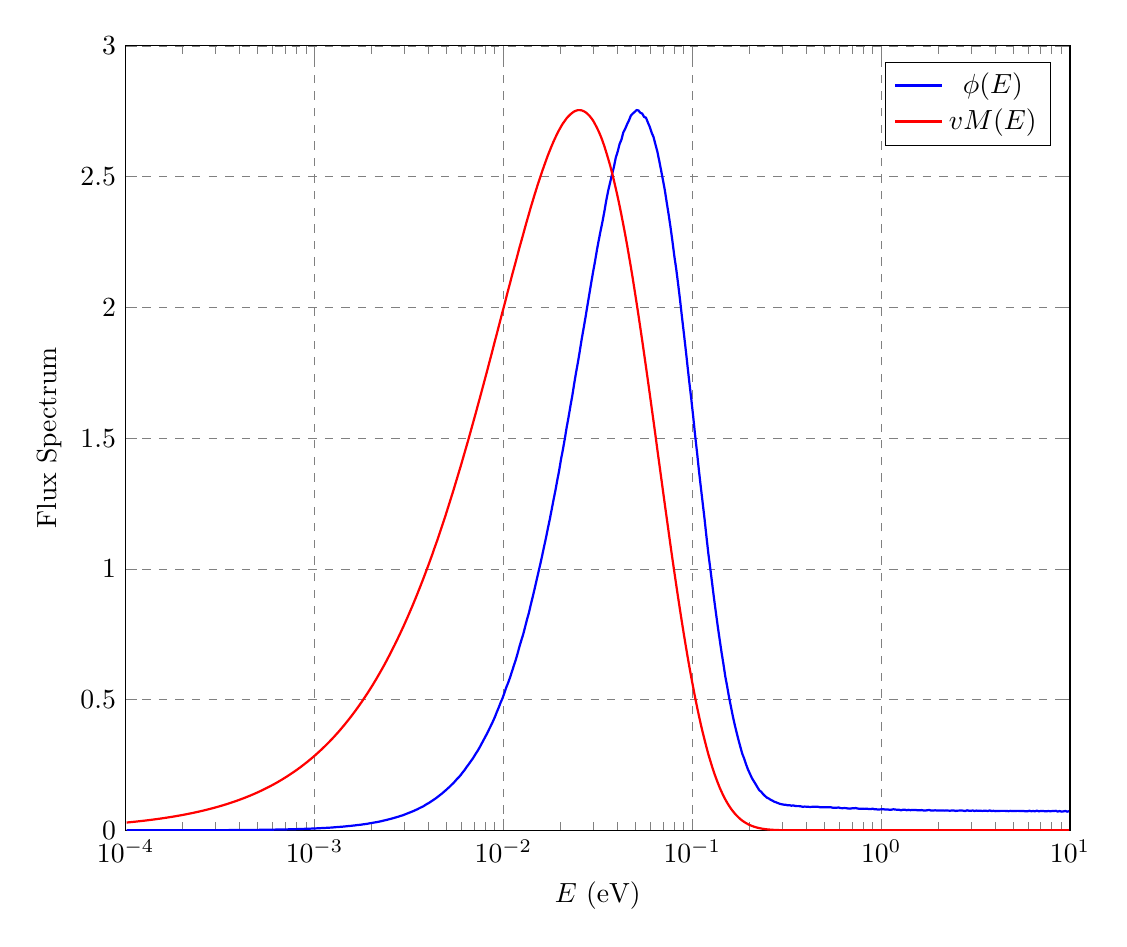
\begin{tikzpicture} \begin{axis}
[scale=1.75, xmode=log,
 xmin=1e-4, xmax=10,
 ymin=0, ymax=3,
 grid=major, 
 major grid style={color=gray,line width=0.2pt, dashed},
 xlabel=$E$ (eV),
 ylabel=Flux Spectrum,
]

\addplot[line width=0.8pt, color=blue] coordinates {
( 1.012e-04 , 7.271e-05 )( 1.035e-04 , 7.982e-05 )( 1.059e-04 , 8.286e-05 )( 1.084e-04 , 8.311e-05 )( 1.109e-04 , 8.922e-05 )( 1.135e-04 , 9.022e-05 )( 1.162e-04 , 1.010e-04 )( 1.189e-04 , 1.042e-04 )( 1.216e-04 , 1.085e-04 )( 1.245e-04 , 1.104e-04 )( 1.274e-04 , 1.204e-04 )( 1.303e-04 , 1.308e-04 )( 1.334e-04 , 1.347e-04 )( 1.365e-04 , 1.333e-04 )( 1.396e-04 , 1.535e-04 )( 1.429e-04 , 1.552e-04 )( 1.462e-04 , 1.679e-04 )( 1.496e-04 , 1.719e-04 )( 1.531e-04 , 1.796e-04 )( 1.567e-04 , 1.759e-04 )( 1.603e-04 , 1.788e-04 )( 1.641e-04 , 2.181e-04 )( 1.679e-04 , 2.113e-04 )( 1.718e-04 , 2.101e-04 )( 1.758e-04 , 2.210e-04 )( 1.799e-04 , 2.356e-04 )( 1.841e-04 , 2.380e-04 )( 1.884e-04 , 2.610e-04 )( 1.928e-04 , 2.869e-04 )( 1.973e-04 , 2.899e-04 )( 2.019e-04 , 3.002e-04 )( 2.066e-04 , 3.064e-04 )( 2.114e-04 , 3.301e-04 )( 2.163e-04 , 3.349e-04 )( 2.213e-04 , 3.566e-04 )( 2.265e-04 , 4.105e-04 )( 2.318e-04 , 3.864e-04 )( 2.372e-04 , 4.188e-04 )( 2.427e-04 , 4.542e-04 )( 2.483e-04 , 4.480e-04 )( 2.541e-04 , 4.842e-04 )( 2.600e-04 , 4.948e-04 )( 2.661e-04 , 5.261e-04 )( 2.723e-04 , 5.676e-04 )( 2.786e-04 , 5.781e-04 )( 2.851e-04 , 5.908e-04 )( 2.918e-04 , 6.376e-04 )( 2.986e-04 , 6.754e-04 )( 3.055e-04 , 6.742e-04 )( 3.126e-04 , 7.177e-04 )( 3.199e-04 , 8.262e-04 )( 3.274e-04 , 8.306e-04 )( 3.350e-04 , 8.715e-04 )( 3.428e-04 , 8.730e-04 )( 3.508e-04 , 9.505e-04 )( 3.589e-04 , 9.783e-04 )( 3.673e-04 , 1.012e-03 )( 3.759e-04 , 1.038e-03 )( 3.846e-04 , 1.092e-03 )( 3.936e-04 , 1.127e-03 )( 4.027e-04 , 1.182e-03 )( 4.121e-04 , 1.223e-03 )( 4.217e-04 , 1.312e-03 )( 4.315e-04 , 1.326e-03 )( 4.416e-04 , 1.466e-03 )( 4.519e-04 , 1.517e-03 )( 4.624e-04 , 1.610e-03 )( 4.732e-04 , 1.634e-03 )( 4.842e-04 , 1.760e-03 )( 4.955e-04 , 1.833e-03 )( 5.070e-04 , 1.888e-03 )( 5.188e-04 , 2.009e-03 )( 5.309e-04 , 2.029e-03 )( 5.433e-04 , 2.128e-03 )( 5.559e-04 , 2.238e-03 )( 5.689e-04 , 2.310e-03 )( 5.821e-04 , 2.455e-03 )( 5.957e-04 , 2.576e-03 )( 6.096e-04 , 2.732e-03 )( 6.238e-04 , 2.888e-03 )( 6.383e-04 , 2.984e-03 )( 6.532e-04 , 3.154e-03 )( 6.684e-04 , 3.239e-03 )( 6.840e-04 , 3.368e-03 )( 6.999e-04 , 3.601e-03 )( 7.162e-04 , 3.688e-03 )( 7.329e-04 , 3.959e-03 )( 7.499e-04 , 4.048e-03 )( 7.674e-04 , 4.287e-03 )( 7.853e-04 , 4.483e-03 )( 8.036e-04 , 4.692e-03 )( 8.223e-04 , 4.953e-03 )( 8.415e-04 , 5.119e-03 )( 8.611e-04 , 5.349e-03 )( 8.811e-04 , 5.689e-03 )( 9.016e-04 , 5.899e-03 )( 9.226e-04 , 6.160e-03 )( 9.441e-04 , 6.437e-03 )( 9.661e-04 , 6.715e-03 )( 9.886e-04 , 7.150e-03 )( 1.012e-03 , 7.353e-03 )( 1.035e-03 , 7.848e-03 )( 1.059e-03 , 8.148e-03 )( 1.084e-03 , 8.580e-03 )( 1.109e-03 , 8.775e-03 )( 1.135e-03 , 9.303e-03 )( 1.162e-03 , 9.678e-03 )( 1.189e-03 , 1.019e-02 )( 1.216e-03 , 1.051e-02 )( 1.245e-03 , 1.104e-02 )( 1.274e-03 , 1.171e-02 )( 1.303e-03 , 1.234e-02 )( 1.334e-03 , 1.275e-02 )( 1.365e-03 , 1.344e-02 )( 1.396e-03 , 1.394e-02 )( 1.429e-03 , 1.450e-02 )( 1.462e-03 , 1.525e-02 )( 1.496e-03 , 1.609e-02 )( 1.531e-03 , 1.678e-02 )( 1.567e-03 , 1.734e-02 )( 1.603e-03 , 1.832e-02 )( 1.641e-03 , 1.900e-02 )( 1.679e-03 , 2.017e-02 )( 1.718e-03 , 2.077e-02 )( 1.758e-03 , 2.157e-02 )( 1.799e-03 , 2.279e-02 )( 1.841e-03 , 2.361e-02 )( 1.884e-03 , 2.468e-02 )( 1.928e-03 , 2.587e-02 )( 1.973e-03 , 2.736e-02 )( 2.019e-03 , 2.848e-02 )( 2.066e-03 , 2.989e-02 )( 2.114e-03 , 3.099e-02 )( 2.163e-03 , 3.230e-02 )( 2.213e-03 , 3.370e-02 )( 2.265e-03 , 3.538e-02 )( 2.318e-03 , 3.722e-02 )( 2.372e-03 , 3.884e-02 )( 2.427e-03 , 4.051e-02 )( 2.483e-03 , 4.249e-02 )( 2.541e-03 , 4.426e-02 )( 2.600e-03 , 4.623e-02 )( 2.661e-03 , 4.835e-02 )( 2.723e-03 , 5.048e-02 )( 2.786e-03 , 5.258e-02 )( 2.851e-03 , 5.517e-02 )( 2.918e-03 , 5.697e-02 )( 2.986e-03 , 5.981e-02 )( 3.055e-03 , 6.274e-02 )( 3.126e-03 , 6.556e-02 )( 3.199e-03 , 6.839e-02 )( 3.274e-03 , 7.124e-02 )( 3.350e-03 , 7.418e-02 )( 3.428e-03 , 7.759e-02 )( 3.508e-03 , 8.093e-02 )( 3.589e-03 , 8.470e-02 )( 3.673e-03 , 8.823e-02 )( 3.759e-03 , 9.145e-02 )( 3.846e-03 , 9.608e-02 )( 3.936e-03 , 1.007e-01 )( 4.027e-03 , 1.043e-01 )( 4.121e-03 , 1.093e-01 )( 4.217e-03 , 1.142e-01 )( 4.315e-03 , 1.188e-01 )( 4.416e-03 , 1.240e-01 )( 4.519e-03 , 1.295e-01 )( 4.624e-03 , 1.354e-01 )( 4.732e-03 , 1.408e-01 )( 4.842e-03 , 1.472e-01 )( 4.955e-03 , 1.533e-01 )( 5.070e-03 , 1.601e-01 )( 5.188e-03 , 1.664e-01 )( 5.309e-03 , 1.738e-01 )( 5.433e-03 , 1.805e-01 )( 5.559e-03 , 1.885e-01 )( 5.689e-03 , 1.969e-01 )( 5.821e-03 , 2.039e-01 )( 5.957e-03 , 2.124e-01 )( 6.096e-03 , 2.221e-01 )( 6.238e-03 , 2.312e-01 )( 6.383e-03 , 2.418e-01 )( 6.532e-03 , 2.513e-01 )( 6.684e-03 , 2.615e-01 )( 6.840e-03 , 2.716e-01 )( 6.999e-03 , 2.826e-01 )( 7.162e-03 , 2.946e-01 )( 7.329e-03 , 3.056e-01 )( 7.499e-03 , 3.181e-01 )( 7.674e-03 , 3.317e-01 )( 7.853e-03 , 3.452e-01 )( 8.036e-03 , 3.588e-01 )( 8.223e-03 , 3.721e-01 )( 8.415e-03 , 3.873e-01 )( 8.611e-03 , 4.020e-01 )( 8.811e-03 , 4.173e-01 )( 9.016e-03 , 4.334e-01 )( 9.226e-03 , 4.520e-01 )( 9.441e-03 , 4.690e-01 )( 9.661e-03 , 4.881e-01 )( 9.886e-03 , 5.045e-01 )( 1.012e-02 , 5.250e-01 )( 1.035e-02 , 5.461e-01 )( 1.059e-02 , 5.637e-01 )( 1.084e-02 , 5.841e-01 )( 1.109e-02 , 6.062e-01 )( 1.135e-02 , 6.290e-01 )( 1.162e-02 , 6.512e-01 )( 1.189e-02 , 6.761e-01 )( 1.216e-02 , 7.024e-01 )( 1.245e-02 , 7.271e-01 )( 1.274e-02 , 7.502e-01 )( 1.303e-02 , 7.777e-01 )( 1.334e-02 , 8.064e-01 )( 1.365e-02 , 8.319e-01 )( 1.396e-02 , 8.623e-01 )( 1.429e-02 , 8.918e-01 )( 1.462e-02 , 9.222e-01 )( 1.496e-02 , 9.538e-01 )( 1.531e-02 , 9.854e-01 )( 1.567e-02 , 1.017e+00 )( 1.603e-02 , 1.049e+00 )( 1.641e-02 , 1.084e+00 )( 1.679e-02 , 1.117e+00 )( 1.718e-02 , 1.153e+00 )( 1.758e-02 , 1.187e+00 )( 1.799e-02 , 1.224e+00 )( 1.841e-02 , 1.262e+00 )( 1.884e-02 , 1.298e+00 )( 1.928e-02 , 1.338e+00 )( 1.973e-02 , 1.375e+00 )( 2.019e-02 , 1.419e+00 )( 2.066e-02 , 1.456e+00 )( 2.114e-02 , 1.497e+00 )( 2.163e-02 , 1.541e+00 )( 2.213e-02 , 1.580e+00 )( 2.265e-02 , 1.623e+00 )( 2.318e-02 , 1.663e+00 )( 2.372e-02 , 1.709e+00 )( 2.427e-02 , 1.752e+00 )( 2.483e-02 , 1.791e+00 )( 2.541e-02 , 1.835e+00 )( 2.600e-02 , 1.880e+00 )( 2.661e-02 , 1.921e+00 )( 2.723e-02 , 1.963e+00 )( 2.786e-02 , 2.007e+00 )( 2.851e-02 , 2.050e+00 )( 2.918e-02 , 2.094e+00 )( 2.986e-02 , 2.136e+00 )( 3.055e-02 , 2.175e+00 )( 3.126e-02 , 2.218e+00 )( 3.199e-02 , 2.257e+00 )( 3.274e-02 , 2.294e+00 )( 3.350e-02 , 2.329e+00 )( 3.428e-02 , 2.368e+00 )( 3.508e-02 , 2.410e+00 )( 3.589e-02 , 2.446e+00 )( 3.673e-02 , 2.477e+00 )( 3.759e-02 , 2.507e+00 )( 3.846e-02 , 2.536e+00 )( 3.936e-02 , 2.572e+00 )( 4.027e-02 , 2.595e+00 )( 4.121e-02 , 2.624e+00 )( 4.217e-02 , 2.641e+00 )( 4.315e-02 , 2.669e+00 )( 4.416e-02 , 2.683e+00 )( 4.519e-02 , 2.700e+00 )( 4.624e-02 , 2.715e+00 )( 4.732e-02 , 2.733e+00 )( 4.842e-02 , 2.741e+00 )( 4.955e-02 , 2.747e+00 )( 5.070e-02 , 2.754e+00 )( 5.188e-02 , 2.753e+00 )( 5.309e-02 , 2.744e+00 )( 5.433e-02 , 2.741e+00 )( 5.559e-02 , 2.728e+00 )( 5.689e-02 , 2.725e+00 )( 5.821e-02 , 2.707e+00 )( 5.957e-02 , 2.690e+00 )( 6.096e-02 , 2.668e+00 )( 6.238e-02 , 2.651e+00 )( 6.383e-02 , 2.623e+00 )( 6.532e-02 , 2.596e+00 )( 6.684e-02 , 2.561e+00 )( 6.840e-02 , 2.524e+00 )( 6.999e-02 , 2.486e+00 )( 7.162e-02 , 2.447e+00 )( 7.329e-02 , 2.400e+00 )( 7.499e-02 , 2.355e+00 )( 7.674e-02 , 2.306e+00 )( 7.853e-02 , 2.253e+00 )( 8.036e-02 , 2.196e+00 )( 8.223e-02 , 2.147e+00 )( 8.415e-02 , 2.090e+00 )( 8.611e-02 , 2.030e+00 )( 8.811e-02 , 1.966e+00 )( 9.016e-02 , 1.904e+00 )( 9.226e-02 , 1.841e+00 )( 9.441e-02 , 1.775e+00 )( 9.661e-02 , 1.710e+00 )( 9.886e-02 , 1.648e+00 )( 1.012e-01 , 1.581e+00 )( 1.035e-01 , 1.512e+00 )( 1.059e-01 , 1.448e+00 )( 1.084e-01 , 1.378e+00 )( 1.109e-01 , 1.315e+00 )( 1.135e-01 , 1.253e+00 )( 1.162e-01 , 1.190e+00 )( 1.189e-01 , 1.123e+00 )( 1.216e-01 , 1.060e+00 )( 1.245e-01 , 1.003e+00 )( 1.274e-01 , 9.453e-01 )( 1.303e-01 , 8.881e-01 )( 1.334e-01 , 8.328e-01 )( 1.365e-01 , 7.793e-01 )( 1.396e-01 , 7.308e-01 )( 1.429e-01 , 6.810e-01 )( 1.462e-01 , 6.365e-01 )( 1.496e-01 , 5.886e-01 )( 1.531e-01 , 5.499e-01 )( 1.567e-01 , 5.079e-01 )( 1.603e-01 , 4.723e-01 )( 1.641e-01 , 4.356e-01 )( 1.679e-01 , 4.034e-01 )( 1.718e-01 , 3.737e-01 )( 1.758e-01 , 3.452e-01 )( 1.799e-01 , 3.183e-01 )( 1.841e-01 , 2.924e-01 )( 1.884e-01 , 2.740e-01 )( 1.928e-01 , 2.520e-01 )( 1.973e-01 , 2.327e-01 )( 2.019e-01 , 2.168e-01 )( 2.066e-01 , 2.008e-01 )( 2.114e-01 , 1.889e-01 )( 2.163e-01 , 1.773e-01 )( 2.213e-01 , 1.649e-01 )( 2.265e-01 , 1.532e-01 )( 2.318e-01 , 1.475e-01 )( 2.372e-01 , 1.385e-01 )( 2.427e-01 , 1.316e-01 )( 2.483e-01 , 1.253e-01 )( 2.541e-01 , 1.218e-01 )( 2.600e-01 , 1.169e-01 )( 2.661e-01 , 1.134e-01 )( 2.723e-01 , 1.092e-01 )( 2.786e-01 , 1.068e-01 )( 2.851e-01 , 1.039e-01 )( 2.918e-01 , 1.010e-01 )( 2.986e-01 , 9.968e-02 )( 3.055e-01 , 9.814e-02 )( 3.126e-01 , 9.781e-02 )( 3.199e-01 , 9.571e-02 )( 3.274e-01 , 9.624e-02 )( 3.350e-01 , 9.433e-02 )( 3.428e-01 , 9.515e-02 )( 3.508e-01 , 9.342e-02 )( 3.589e-01 , 9.262e-02 )( 3.673e-01 , 9.275e-02 )( 3.759e-01 , 9.166e-02 )( 3.846e-01 , 9.009e-02 )( 3.936e-01 , 9.092e-02 )( 4.027e-01 , 9.041e-02 )( 4.121e-01 , 8.997e-02 )( 4.217e-01 , 8.952e-02 )( 4.315e-01 , 8.996e-02 )( 4.416e-01 , 8.993e-02 )( 4.519e-01 , 8.999e-02 )( 4.624e-01 , 9.021e-02 )( 4.732e-01 , 8.863e-02 )( 4.842e-01 , 8.856e-02 )( 4.955e-01 , 8.802e-02 )( 5.070e-01 , 8.879e-02 )( 5.188e-01 , 8.825e-02 )( 5.309e-01 , 8.810e-02 )( 5.433e-01 , 8.800e-02 )( 5.559e-01 , 8.646e-02 )( 5.689e-01 , 8.677e-02 )( 5.821e-01 , 8.666e-02 )( 5.957e-01 , 8.729e-02 )( 6.096e-01 , 8.515e-02 )( 6.238e-01 , 8.478e-02 )( 6.383e-01 , 8.524e-02 )( 6.532e-01 , 8.490e-02 )( 6.684e-01 , 8.357e-02 )( 6.840e-01 , 8.304e-02 )( 6.999e-01 , 8.422e-02 )( 7.162e-01 , 8.411e-02 )( 7.329e-01 , 8.544e-02 )( 7.499e-01 , 8.350e-02 )( 7.674e-01 , 8.262e-02 )( 7.853e-01 , 8.240e-02 )( 8.036e-01 , 8.239e-02 )( 8.223e-01 , 8.216e-02 )( 8.415e-01 , 8.292e-02 )( 8.611e-01 , 8.134e-02 )( 8.811e-01 , 8.121e-02 )( 9.016e-01 , 8.291e-02 )( 9.226e-01 , 8.045e-02 )( 9.441e-01 , 8.051e-02 )( 9.661e-01 , 7.943e-02 )( 9.886e-01 , 8.020e-02 )( 1.012e+00 , 8.072e-02 )( 1.035e+00 , 8.054e-02 )( 1.059e+00 , 7.931e-02 )( 1.084e+00 , 7.982e-02 )( 1.109e+00 , 7.870e-02 )( 1.135e+00 , 7.915e-02 )( 1.162e+00 , 8.069e-02 )( 1.189e+00 , 7.949e-02 )( 1.216e+00 , 7.877e-02 )( 1.245e+00 , 7.866e-02 )( 1.274e+00 , 7.681e-02 )( 1.303e+00 , 7.870e-02 )( 1.334e+00 , 7.913e-02 )( 1.365e+00 , 7.701e-02 )( 1.396e+00 , 7.842e-02 )( 1.429e+00 , 7.709e-02 )( 1.462e+00 , 7.828e-02 )( 1.496e+00 , 7.772e-02 )( 1.531e+00 , 7.764e-02 )( 1.567e+00 , 7.649e-02 )( 1.603e+00 , 7.670e-02 )( 1.641e+00 , 7.752e-02 )( 1.679e+00 , 7.592e-02 )( 1.718e+00 , 7.580e-02 )( 1.758e+00 , 7.718e-02 )( 1.799e+00 , 7.771e-02 )( 1.841e+00 , 7.568e-02 )( 1.884e+00 , 7.580e-02 )( 1.928e+00 , 7.666e-02 )( 1.973e+00 , 7.606e-02 )( 2.019e+00 , 7.615e-02 )( 2.066e+00 , 7.632e-02 )( 2.114e+00 , 7.600e-02 )( 2.163e+00 , 7.539e-02 )( 2.213e+00 , 7.609e-02 )( 2.265e+00 , 7.555e-02 )( 2.318e+00 , 7.514e-02 )( 2.372e+00 , 7.597e-02 )( 2.427e+00 , 7.593e-02 )( 2.483e+00 , 7.425e-02 )( 2.541e+00 , 7.530e-02 )( 2.600e+00 , 7.561e-02 )( 2.661e+00 , 7.602e-02 )( 2.723e+00 , 7.517e-02 )( 2.786e+00 , 7.394e-02 )( 2.851e+00 , 7.665e-02 )( 2.918e+00 , 7.501e-02 )( 2.986e+00 , 7.472e-02 )( 3.055e+00 , 7.604e-02 )( 3.126e+00 , 7.411e-02 )( 3.199e+00 , 7.564e-02 )( 3.274e+00 , 7.465e-02 )( 3.350e+00 , 7.524e-02 )( 3.428e+00 , 7.427e-02 )( 3.508e+00 , 7.487e-02 )( 3.589e+00 , 7.477e-02 )( 3.673e+00 , 7.401e-02 )( 3.759e+00 , 7.597e-02 )( 3.846e+00 , 7.416e-02 )( 3.936e+00 , 7.472e-02 )( 4.027e+00 , 7.343e-02 )( 4.121e+00 , 7.445e-02 )( 4.217e+00 , 7.431e-02 )( 4.315e+00 , 7.451e-02 )( 4.416e+00 , 7.446e-02 )( 4.519e+00 , 7.451e-02 )( 4.624e+00 , 7.387e-02 )( 4.732e+00 , 7.344e-02 )( 4.842e+00 , 7.456e-02 )( 4.955e+00 , 7.421e-02 )( 5.070e+00 , 7.414e-02 )( 5.188e+00 , 7.431e-02 )( 5.309e+00 , 7.453e-02 )( 5.433e+00 , 7.389e-02 )( 5.559e+00 , 7.404e-02 )( 5.689e+00 , 7.395e-02 )( 5.821e+00 , 7.281e-02 )( 5.957e+00 , 7.309e-02 )( 6.096e+00 , 7.482e-02 )( 6.238e+00 , 7.318e-02 )( 6.383e+00 , 7.387e-02 )( 6.532e+00 , 7.295e-02 )( 6.684e+00 , 7.524e-02 )( 6.840e+00 , 7.284e-02 )( 6.999e+00 , 7.427e-02 )( 7.162e+00 , 7.418e-02 )( 7.329e+00 , 7.334e-02 )( 7.499e+00 , 7.263e-02 )( 7.674e+00 , 7.396e-02 )( 7.853e+00 , 7.312e-02 )( 8.036e+00 , 7.371e-02 )( 8.223e+00 , 7.402e-02 )( 8.415e+00 , 7.465e-02 )( 8.611e+00 , 7.191e-02 )( 8.811e+00 , 7.384e-02 )( 9.016e+00 , 7.163e-02 )( 9.226e+00 , 7.254e-02 )( 9.441e+00 , 7.415e-02 )( 9.661e+00 , 7.155e-02 )( 9.886e+00 , 7.316e-02 )
};

\addplot[line width=0.8pt, color=red] coordinates {
( 1.012e-04 , 2.988e-02 )( 1.035e-04 , 3.057e-02 )( 1.059e-04 , 3.128e-02 )( 1.084e-04 , 3.200e-02 )( 1.109e-04 , 3.275e-02 )( 1.135e-04 , 3.351e-02 )( 1.162e-04 , 3.428e-02 )( 1.189e-04 , 3.508e-02 )( 1.216e-04 , 3.589e-02 )( 1.245e-04 , 3.672e-02 )( 1.274e-04 , 3.757e-02 )( 1.303e-04 , 3.844e-02 )( 1.334e-04 , 3.933e-02 )( 1.365e-04 , 4.025e-02 )( 1.396e-04 , 4.118e-02 )( 1.429e-04 , 4.213e-02 )( 1.462e-04 , 4.311e-02 )( 1.496e-04 , 4.411e-02 )( 1.531e-04 , 4.513e-02 )( 1.567e-04 , 4.617e-02 )( 1.603e-04 , 4.724e-02 )( 1.641e-04 , 4.833e-02 )( 1.679e-04 , 4.945e-02 )( 1.718e-04 , 5.060e-02 )( 1.758e-04 , 5.177e-02 )( 1.799e-04 , 5.296e-02 )( 1.841e-04 , 5.419e-02 )( 1.884e-04 , 5.544e-02 )( 1.928e-04 , 5.672e-02 )( 1.973e-04 , 5.803e-02 )( 2.019e-04 , 5.937e-02 )( 2.066e-04 , 6.075e-02 )( 2.114e-04 , 6.215e-02 )( 2.163e-04 , 6.358e-02 )( 2.213e-04 , 6.505e-02 )( 2.265e-04 , 6.655e-02 )( 2.318e-04 , 6.809e-02 )( 2.372e-04 , 6.966e-02 )( 2.427e-04 , 7.127e-02 )( 2.483e-04 , 7.291e-02 )( 2.541e-04 , 7.459e-02 )( 2.600e-04 , 7.631e-02 )( 2.661e-04 , 7.807e-02 )( 2.723e-04 , 7.987e-02 )( 2.786e-04 , 8.171e-02 )( 2.851e-04 , 8.359e-02 )( 2.918e-04 , 8.552e-02 )( 2.986e-04 , 8.749e-02 )( 3.055e-04 , 8.950e-02 )( 3.126e-04 , 9.156e-02 )( 3.199e-04 , 9.366e-02 )( 3.274e-04 , 9.582e-02 )( 3.350e-04 , 9.802e-02 )( 3.428e-04 , 1.003e-01 )( 3.508e-04 , 1.026e-01 )( 3.589e-04 , 1.049e-01 )( 3.673e-04 , 1.073e-01 )( 3.759e-04 , 1.098e-01 )( 3.846e-04 , 1.123e-01 )( 3.936e-04 , 1.149e-01 )( 4.027e-04 , 1.175e-01 )( 4.121e-04 , 1.202e-01 )( 4.217e-04 , 1.230e-01 )( 4.315e-04 , 1.258e-01 )( 4.416e-04 , 1.287e-01 )( 4.519e-04 , 1.316e-01 )( 4.624e-04 , 1.346e-01 )( 4.732e-04 , 1.377e-01 )( 4.842e-04 , 1.408e-01 )( 4.955e-04 , 1.441e-01 )( 5.070e-04 , 1.473e-01 )( 5.188e-04 , 1.507e-01 )( 5.309e-04 , 1.541e-01 )( 5.433e-04 , 1.577e-01 )( 5.559e-04 , 1.613e-01 )( 5.689e-04 , 1.649e-01 )( 5.821e-04 , 1.687e-01 )( 5.957e-04 , 1.725e-01 )( 6.096e-04 , 1.764e-01 )( 6.238e-04 , 1.804e-01 )( 6.383e-04 , 1.845e-01 )( 6.532e-04 , 1.887e-01 )( 6.684e-04 , 1.930e-01 )( 6.840e-04 , 1.974e-01 )( 6.999e-04 , 2.019e-01 )( 7.162e-04 , 2.064e-01 )( 7.329e-04 , 2.111e-01 )( 7.499e-04 , 2.159e-01 )( 7.674e-04 , 2.207e-01 )( 7.853e-04 , 2.257e-01 )( 8.036e-04 , 2.308e-01 )( 8.223e-04 , 2.360e-01 )( 8.415e-04 , 2.413e-01 )( 8.611e-04 , 2.468e-01 )( 8.811e-04 , 2.523e-01 )( 9.016e-04 , 2.580e-01 )( 9.226e-04 , 2.638e-01 )( 9.441e-04 , 2.697e-01 )( 9.661e-04 , 2.757e-01 )( 9.886e-04 , 2.819e-01 )( 1.012e-03 , 2.882e-01 )( 1.035e-03 , 2.946e-01 )( 1.059e-03 , 3.012e-01 )( 1.084e-03 , 3.079e-01 )( 1.109e-03 , 3.148e-01 )( 1.135e-03 , 3.218e-01 )( 1.162e-03 , 3.289e-01 )( 1.189e-03 , 3.362e-01 )( 1.216e-03 , 3.437e-01 )( 1.245e-03 , 3.513e-01 )( 1.274e-03 , 3.591e-01 )( 1.303e-03 , 3.670e-01 )( 1.334e-03 , 3.751e-01 )( 1.365e-03 , 3.834e-01 )( 1.396e-03 , 3.918e-01 )( 1.429e-03 , 4.004e-01 )( 1.462e-03 , 4.092e-01 )( 1.496e-03 , 4.182e-01 )( 1.531e-03 , 4.273e-01 )( 1.567e-03 , 4.366e-01 )( 1.603e-03 , 4.462e-01 )( 1.641e-03 , 4.559e-01 )( 1.679e-03 , 4.658e-01 )( 1.718e-03 , 4.759e-01 )( 1.758e-03 , 4.862e-01 )( 1.799e-03 , 4.967e-01 )( 1.841e-03 , 5.075e-01 )( 1.884e-03 , 5.184e-01 )( 1.928e-03 , 5.296e-01 )( 1.973e-03 , 5.409e-01 )( 2.019e-03 , 5.525e-01 )( 2.066e-03 , 5.643e-01 )( 2.114e-03 , 5.764e-01 )( 2.163e-03 , 5.887e-01 )( 2.213e-03 , 6.012e-01 )( 2.265e-03 , 6.139e-01 )( 2.318e-03 , 6.269e-01 )( 2.372e-03 , 6.401e-01 )( 2.427e-03 , 6.536e-01 )( 2.483e-03 , 6.674e-01 )( 2.541e-03 , 6.813e-01 )( 2.600e-03 , 6.956e-01 )( 2.661e-03 , 7.101e-01 )( 2.723e-03 , 7.248e-01 )( 2.786e-03 , 7.399e-01 )( 2.851e-03 , 7.551e-01 )( 2.918e-03 , 7.707e-01 )( 2.986e-03 , 7.865e-01 )( 3.055e-03 , 8.026e-01 )( 3.126e-03 , 8.190e-01 )( 3.199e-03 , 8.357e-01 )( 3.274e-03 , 8.526e-01 )( 3.350e-03 , 8.699e-01 )( 3.428e-03 , 8.874e-01 )( 3.508e-03 , 9.052e-01 )( 3.589e-03 , 9.233e-01 )( 3.673e-03 , 9.417e-01 )( 3.759e-03 , 9.603e-01 )( 3.846e-03 , 9.793e-01 )( 3.936e-03 , 9.986e-01 )( 4.027e-03 , 1.018e+00 )( 4.121e-03 , 1.038e+00 )( 4.217e-03 , 1.058e+00 )( 4.315e-03 , 1.079e+00 )( 4.416e-03 , 1.099e+00 )( 4.519e-03 , 1.120e+00 )( 4.624e-03 , 1.142e+00 )( 4.732e-03 , 1.163e+00 )( 4.842e-03 , 1.185e+00 )( 4.955e-03 , 1.207e+00 )( 5.070e-03 , 1.230e+00 )( 5.188e-03 , 1.253e+00 )( 5.309e-03 , 1.276e+00 )( 5.433e-03 , 1.299e+00 )( 5.559e-03 , 1.323e+00 )( 5.689e-03 , 1.347e+00 )( 5.821e-03 , 1.371e+00 )( 5.957e-03 , 1.395e+00 )( 6.096e-03 , 1.420e+00 )( 6.238e-03 , 1.445e+00 )( 6.383e-03 , 1.470e+00 )( 6.532e-03 , 1.495e+00 )( 6.684e-03 , 1.521e+00 )( 6.840e-03 , 1.547e+00 )( 6.999e-03 , 1.573e+00 )( 7.162e-03 , 1.599e+00 )( 7.329e-03 , 1.626e+00 )( 7.499e-03 , 1.652e+00 )( 7.674e-03 , 1.679e+00 )( 7.853e-03 , 1.706e+00 )( 8.036e-03 , 1.733e+00 )( 8.223e-03 , 1.760e+00 )( 8.415e-03 , 1.788e+00 )( 8.611e-03 , 1.815e+00 )( 8.811e-03 , 1.843e+00 )( 9.016e-03 , 1.871e+00 )( 9.226e-03 , 1.898e+00 )( 9.441e-03 , 1.926e+00 )( 9.661e-03 , 1.954e+00 )( 9.886e-03 , 1.982e+00 )( 1.012e-02 , 2.009e+00 )( 1.035e-02 , 2.037e+00 )( 1.059e-02 , 2.065e+00 )( 1.084e-02 , 2.092e+00 )( 1.109e-02 , 2.120e+00 )( 1.135e-02 , 2.147e+00 )( 1.162e-02 , 2.174e+00 )( 1.189e-02 , 2.201e+00 )( 1.216e-02 , 2.228e+00 )( 1.245e-02 , 2.254e+00 )( 1.274e-02 , 2.280e+00 )( 1.303e-02 , 2.306e+00 )( 1.334e-02 , 2.332e+00 )( 1.365e-02 , 2.357e+00 )( 1.396e-02 , 2.382e+00 )( 1.429e-02 , 2.406e+00 )( 1.462e-02 , 2.430e+00 )( 1.496e-02 , 2.453e+00 )( 1.531e-02 , 2.476e+00 )( 1.567e-02 , 2.498e+00 )( 1.603e-02 , 2.519e+00 )( 1.641e-02 , 2.540e+00 )( 1.679e-02 , 2.560e+00 )( 1.718e-02 , 2.580e+00 )( 1.758e-02 , 2.598e+00 )( 1.799e-02 , 2.616e+00 )( 1.841e-02 , 2.633e+00 )( 1.884e-02 , 2.649e+00 )( 1.928e-02 , 2.664e+00 )( 1.973e-02 , 2.678e+00 )( 2.019e-02 , 2.691e+00 )( 2.066e-02 , 2.703e+00 )( 2.114e-02 , 2.713e+00 )( 2.163e-02 , 2.723e+00 )( 2.213e-02 , 2.731e+00 )( 2.265e-02 , 2.738e+00 )( 2.318e-02 , 2.744e+00 )( 2.372e-02 , 2.749e+00 )( 2.427e-02 , 2.752e+00 )( 2.483e-02 , 2.754e+00 )( 2.541e-02 , 2.754e+00 )( 2.600e-02 , 2.753e+00 )( 2.661e-02 , 2.750e+00 )( 2.723e-02 , 2.746e+00 )( 2.786e-02 , 2.740e+00 )( 2.851e-02 , 2.733e+00 )( 2.918e-02 , 2.724e+00 )( 2.986e-02 , 2.714e+00 )( 3.055e-02 , 2.701e+00 )( 3.126e-02 , 2.687e+00 )( 3.199e-02 , 2.672e+00 )( 3.274e-02 , 2.655e+00 )( 3.350e-02 , 2.636e+00 )( 3.428e-02 , 2.615e+00 )( 3.508e-02 , 2.592e+00 )( 3.589e-02 , 2.568e+00 )( 3.673e-02 , 2.543e+00 )( 3.759e-02 , 2.515e+00 )( 3.846e-02 , 2.486e+00 )( 3.936e-02 , 2.455e+00 )( 4.027e-02 , 2.423e+00 )( 4.121e-02 , 2.389e+00 )( 4.217e-02 , 2.353e+00 )( 4.315e-02 , 2.316e+00 )( 4.416e-02 , 2.278e+00 )( 4.519e-02 , 2.238e+00 )( 4.624e-02 , 2.196e+00 )( 4.732e-02 , 2.154e+00 )( 4.842e-02 , 2.110e+00 )( 4.955e-02 , 2.064e+00 )( 5.070e-02 , 2.018e+00 )( 5.188e-02 , 1.971e+00 )( 5.309e-02 , 1.922e+00 )( 5.433e-02 , 1.873e+00 )( 5.559e-02 , 1.823e+00 )( 5.689e-02 , 1.772e+00 )( 5.821e-02 , 1.721e+00 )( 5.957e-02 , 1.669e+00 )( 6.096e-02 , 1.616e+00 )( 6.238e-02 , 1.564e+00 )( 6.383e-02 , 1.511e+00 )( 6.532e-02 , 1.457e+00 )( 6.684e-02 , 1.404e+00 )( 6.840e-02 , 1.351e+00 )( 6.999e-02 , 1.298e+00 )( 7.162e-02 , 1.245e+00 )( 7.329e-02 , 1.193e+00 )( 7.499e-02 , 1.141e+00 )( 7.674e-02 , 1.089e+00 )( 7.853e-02 , 1.038e+00 )( 8.036e-02 , 9.882e-01 )( 8.223e-02 , 9.390e-01 )( 8.415e-02 , 8.907e-01 )( 8.611e-02 , 8.433e-01 )( 8.811e-02 , 7.971e-01 )( 9.016e-02 , 7.520e-01 )( 9.226e-02 , 7.081e-01 )( 9.441e-02 , 6.654e-01 )( 9.661e-02 , 6.241e-01 )( 9.886e-02 , 5.842e-01 )( 1.012e-01 , 5.457e-01 )( 1.035e-01 , 5.087e-01 )( 1.059e-01 , 4.731e-01 )( 1.084e-01 , 4.391e-01 )( 1.109e-01 , 4.065e-01 )( 1.135e-01 , 3.755e-01 )( 1.162e-01 , 3.461e-01 )( 1.189e-01 , 3.181e-01 )( 1.216e-01 , 2.917e-01 )( 1.245e-01 , 2.669e-01 )( 1.274e-01 , 2.435e-01 )( 1.303e-01 , 2.215e-01 )( 1.334e-01 , 2.010e-01 )( 1.365e-01 , 1.819e-01 )( 1.396e-01 , 1.641e-01 )( 1.429e-01 , 1.476e-01 )( 1.462e-01 , 1.324e-01 )( 1.496e-01 , 1.184e-01 )( 1.531e-01 , 1.055e-01 )( 1.567e-01 , 9.375e-02 )( 1.603e-01 , 8.302e-02 )( 1.641e-01 , 7.328e-02 )( 1.679e-01 , 6.445e-02 )( 1.718e-01 , 5.649e-02 )( 1.758e-01 , 4.933e-02 )( 1.799e-01 , 4.292e-02 )( 1.841e-01 , 3.721e-02 )( 1.884e-01 , 3.213e-02 )( 1.928e-01 , 2.763e-02 )( 1.973e-01 , 2.367e-02 )( 2.019e-01 , 2.019e-02 )( 2.066e-01 , 1.715e-02 )( 2.114e-01 , 1.450e-02 )( 2.163e-01 , 1.221e-02 )( 2.213e-01 , 1.024e-02 )( 2.265e-01 , 8.540e-03 )( 2.318e-01 , 7.091e-03 )( 2.372e-01 , 5.860e-03 )( 2.427e-01 , 4.818e-03 )( 2.483e-01 , 3.941e-03 )( 2.541e-01 , 3.207e-03 )( 2.600e-01 , 2.596e-03 )( 2.661e-01 , 2.090e-03 )( 2.723e-01 , 1.673e-03 )( 2.786e-01 , 1.332e-03 )( 2.851e-01 , 1.054e-03 )( 2.918e-01 , 8.290e-04 )( 2.986e-01 , 6.481e-04 )( 3.055e-01 , 5.036e-04 )( 3.126e-01 , 3.887e-04 )( 3.199e-01 , 2.981e-04 )( 3.274e-01 , 2.271e-04 )( 3.350e-01 , 1.718e-04 )( 3.428e-01 , 1.291e-04 )( 3.508e-01 , 9.627e-05 )( 3.589e-01 , 7.128e-05 )( 3.673e-01 , 5.238e-05 )( 3.759e-01 , 3.819e-05 )( 3.846e-01 , 2.763e-05 )( 3.936e-01 , 1.983e-05 )( 4.027e-01 , 1.411e-05 )( 4.121e-01 , 9.960e-06 )( 4.217e-01 , 6.968e-06 )( 4.315e-01 , 4.832e-06 )( 4.416e-01 , 3.321e-06 )( 4.519e-01 , 2.261e-06 )( 4.624e-01 , 1.525e-06 )( 4.732e-01 , 1.019e-06 )( 4.842e-01 , 6.736e-07 )( 4.955e-01 , 4.410e-07 )( 5.070e-01 , 2.857e-07 )( 5.188e-01 , 1.831e-07 )( 5.309e-01 , 1.161e-07 )( 5.433e-01 , 7.281e-08 )( 5.559e-01 , 4.513e-08 )( 5.689e-01 , 2.765e-08 )( 5.821e-01 , 1.674e-08 )( 5.957e-01 , 1.001e-08 )( 6.096e-01 , 5.915e-09 )( 6.238e-01 , 3.449e-09 )( 6.383e-01 , 1.985e-09 )( 6.532e-01 , 1.127e-09 )( 6.684e-01 , 6.315e-10 )( 6.840e-01 , 3.488e-10 )( 6.999e-01 , 1.899e-10 )( 7.162e-01 , 1.019e-10 )( 7.329e-01 , 5.385e-11 )( 7.499e-01 , 2.802e-11 )( 7.674e-01 , 1.436e-11 )( 7.853e-01 , 7.238e-12 )( 8.036e-01 , 3.589e-12 )( 8.223e-01 , 1.750e-12 )( 8.415e-01 , 8.386e-13 )( 8.611e-01 , 3.948e-13 )( 8.811e-01 , 1.826e-13 )( 9.016e-01 , 8.287e-14 )( 9.226e-01 , 3.691e-14 )( 9.441e-01 , 1.613e-14 )( 9.661e-01 , 6.906e-15 )( 9.886e-01 , 2.898e-15 )( 1.012e+00 , 1.191e-15 )( 1.035e+00 , 4.795e-16 )( 1.059e+00 , 1.888e-16 )( 1.084e+00 , 7.270e-17 )( 1.109e+00 , 2.737e-17 )( 1.135e+00 , 1.007e-17 )( 1.162e+00 , 3.614e-18 )( 1.189e+00 , 1.267e-18 )( 1.216e+00 , 4.330e-19 )( 1.245e+00 , 1.443e-19 )( 1.274e+00 , 4.683e-20 )( 1.303e+00 , 1.480e-20 )( 1.334e+00 , 4.551e-21 )( 1.365e+00 , 1.361e-21 )( 1.396e+00 , 3.954e-22 )( 1.429e+00 , 1.116e-22 )( 1.462e+00 , 3.055e-23 )( 1.496e+00 , 8.112e-24 )( 1.531e+00 , 2.087e-24 )( 1.567e+00 , 5.201e-25 )( 1.603e+00 , 1.254e-25 )( 1.641e+00 , 2.924e-26 )( 1.679e+00 , 6.586e-27 )( 1.718e+00 , 1.432e-27 )( 1.758e+00 , 3.003e-28 )( 1.799e+00 , 6.071e-29 )( 1.841e+00 , 1.182e-29 )( 1.884e+00 , 2.213e-30 )( 1.928e+00 , 3.982e-31 )( 1.973e+00 , 6.884e-32 )( 2.019e+00 , 1.142e-32 )( 2.066e+00 , 1.815e-33 )( 2.114e+00 , 2.762e-34 )( 2.163e+00 , 4.021e-35 )( 2.213e+00 , 5.595e-36 )( 2.265e+00 , 7.432e-37 )( 2.318e+00 , 9.412e-38 )( 2.372e+00 , 1.135e-38 )( 2.427e+00 , 1.303e-39 )( 2.483e+00 , 1.421e-40 )( 2.541e+00 , 1.471e-41 )( 2.600e+00 , 1.444e-42 )( 2.661e+00 , 1.342e-43 )( 2.723e+00 , 1.179e-44 )( 2.786e+00 , 9.789e-46 )( 2.851e+00 , 7.663e-47 )( 2.918e+00 , 5.650e-48 )( 2.986e+00 , 3.918e-49 )( 3.055e+00 , 2.552e-50 )( 3.126e+00 , 1.559e-51 )( 3.199e+00 , 8.918e-53 )( 3.274e+00 , 4.770e-54 )( 3.350e+00 , 2.382e-55 )( 3.428e+00 , 1.109e-56 )( 3.508e+00 , 4.802e-58 )( 3.589e+00 , 1.932e-59 )( 3.673e+00 , 7.209e-61 )( 3.759e+00 , 2.490e-62 )( 3.846e+00 , 7.949e-64 )( 3.936e+00 , 2.341e-65 )( 4.027e+00 , 6.345e-67 )( 4.121e+00 , 1.581e-68 )( 4.217e+00 , 3.611e-70 )( 4.315e+00 , 7.550e-72 )( 4.416e+00 , 1.442e-73 )( 4.519e+00 , 2.510e-75 )( 4.624e+00 , 3.973e-77 )( 4.732e+00 , 5.708e-79 )( 4.842e+00 , 7.424e-81 )( 4.955e+00 , 8.723e-83 )( 5.070e+00 , 9.236e-85 )( 5.188e+00 , 8.791e-87 )( 5.309e+00 , 7.504e-89 )( 5.433e+00 , 5.730e-91 )( 5.559e+00 , 3.903e-93 )( 5.689e+00 , 2.366e-95 )( 5.821e+00 , 1.273e-97 )( 5.957e+00 , 6.059e-100 )( 6.096e+00 , 2.545e-102 )( 6.238e+00 , 9.405e-105 )( 6.383e+00 , 3.049e-107 )( 6.532e+00 , 8.645e-110 )( 6.684e+00 , 2.137e-112 )( 6.840e+00 , 4.590e-115 )( 6.999e+00 , 8.542e-118 )( 7.162e+00 , 1.372e-120 )( 7.329e+00 , 1.897e-123 )( 7.499e+00 , 2.247e-126 )( 7.674e+00 , 2.275e-129 )( 7.853e+00 , 1.960e-132 )( 8.036e+00 , 1.432e-135 )( 8.223e+00 , 8.839e-139 )( 8.415e+00 , 4.590e-142 )( 8.611e+00 , 1.998e-145 )( 8.811e+00 , 7.256e-149 )( 9.016e+00 , 2.190e-152 )( 9.226e+00 , 5.471e-156 )( 9.441e+00 , 1.126e-159 )( 9.661e+00 , 1.900e-163 )( 9.886e+00 , 2.618e-167 )
};

\legend{$\phi(E)$,$vM(E)$}
\end{axis}
\end{tikzpicture}
\caption{Comparison of the thermal scalar flux spectrum $\phi(E)$ and the Maxwellian $vM(E)$.}
 \label{Fig:thermalization_thermalFlux}
\end{center}
\end{figure}

%%%%%%%%%%%%%%%%%%%%%%%%%%%%%%%%%%%%%%%%%%%%%%%%%%%%%%%%%%%%%%%%%%%%%%%%%%%%%%%%%%%%%%%%%%%%%%%%%%%%
\section{Lattice Effects}

In the previous sections, we assumed the reactor could be modeled as a homogeneous mixture. While this allowed for a simplified analysis, simply homogenizing the reactor does not yield suitably accurate results. In this section, we discuss how to compute the relevant quantities for the case of an infinite, homogeneous lattice of nuclear fuel pins in moderator.

\subsection{Lattice Unit Cell and the Lumped Model}

Since a reactor is typically large and involves numerous fuel pins, we can, as first cut at least, solve the lattice problem on a single \emph{unit cell} with reflecting boundary conditions on all sides, which is mathematically equivalent to an infinite array of this unit cell. Typically, in a thermal reactor, the fuel pins are situated in a square lattice arrangement, but some designs use a hexagonal one. 

\begin{figure}[tb!]
\begin{center}
\begin{center}
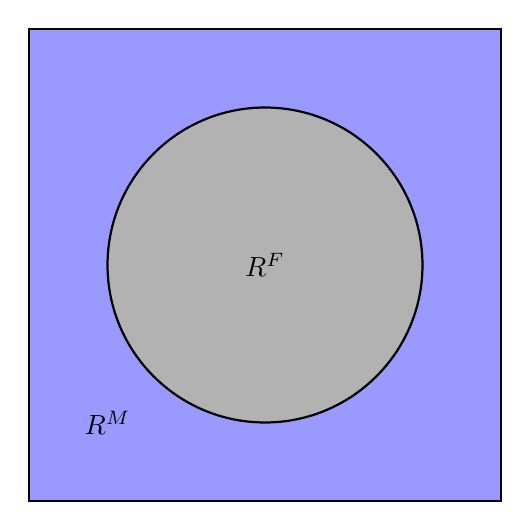
\begin{tikzpicture}
  \filldraw[blue!40] (0,0) -- (0,6) -- (6,6) -- (6,0) -- cycle;
  \filldraw[gray!60] (3,3) circle (2cm);
  \draw[thick] (3,3) circle (2cm);
  \draw[thick] (0,0) -- (0,6) -- (6,6) -- (6,0) -- cycle;
  \node at (3,3) {$R^F$};
  \node at (1,1) {$R^M$};
\end{tikzpicture}
\end{center}
\caption{Depiction of a square lattice unit cell in a nuclear reactor}
\label{Fig:thermalization_squareUnitCell}
\end{center}
\end{figure}

Figure~\ref{Fig:thermalization_squareUnitCell} depicts a unit cell in a square lattice. Here we define the fuel region as $R^F$ and the moderator region as $R^M$. Within each region, we assume the properties, i.e., cross sections, are homogeneous. Mathematically, a cross section takes the form of a piecewise function as
\begin{align}
  \Sigma_x(\pos,E) = \left\{ \begin{array}{l l}
  \Sigma_x^F(E), & \quad \pos \in R^F, \\
  \Sigma_x^M(E), & \quad \pos \in R^M. \\ \end{array} \right. \label{Eq:thermalization_piecewiseLatticeXS}
\end{align}

From this, we then introduce the notion of a lumped model, where we treat quantities to be averages over each individual region. Most important of these is the region-averaged scalar fluxes, which we define as
\begin{align}
  \overline{\phi}^{F/M}(E) = \frac{1}{V^{F/M}} \int_{R^{F/M}} \phi(\pos,E) dV . \label{Eq:thermalization_volumeAveragedFlux}
\end{align}
Here the $F$ superscript denotes the fuel and the $M$ superscript denotes the moderator with the slash being shorthand for either region. In this shorthand, for example, $V^{F/M}$ gives the volume of the fuel $V^F$ or volume of the moderator $V^M$.

We now seek to understand the volume-averaged fluxes in each region. We can describe this by considering four energy ranges:
\begin{enumerate}
  \item The fission range. In this region, the scalar flux in the fuel $\overline{\phi}^F > \overline{\phi}^M$. This is because there is a neutron source in the fuel and these neutrons are primarily removed into the slowing down range via downscattering with the moderator. Note that there is a relatively small amount of fission in this range.
  \item The slowing down range \emph{outside} of resonances. In this region, the fluxes are roughly flat spatially, $\overline{\phi}^F \approx \overline{\phi}^M$. The reason is the only removal mechanism is downscattering (absorption outside resonances is negligible) and this is roughly equal in intensity in either region. Scattering in the fuel does not transfer much energy, but it does do some, so it counts as a removal.
  \item The slowing down range \emph{inside} the resonances. Here, $\overline{\phi}^F \ll \overline{\phi}^M$ because the cross section in the fuel is very large. Essentially any neutron that enters the fuel experiences a collision on the very edge of the pin and many of these neutrons are absorbed.
  \item The thermal range. In this region, $\overline{\phi}^F < \overline{\phi}^M$. This is because the fuel is much more absorbent compared to the moderator.
\end{enumerate}

\begin{figure}[tb!]
\begin{center}
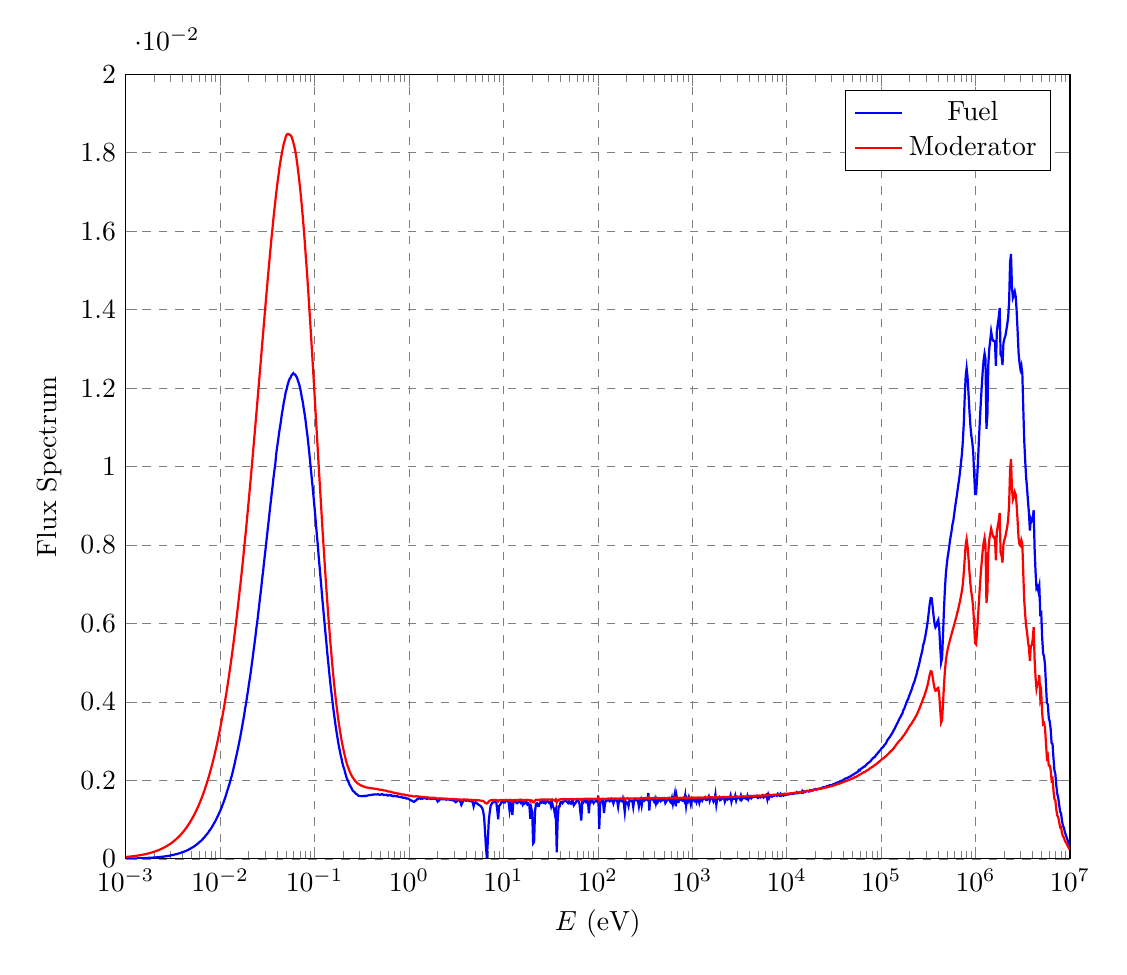
\begin{tikzpicture} \begin{axis}
[scale=1.75, xmode=log,
 xmin=1e-3, xmax=1e7,
 ymin=0, ymax=0.02,
 grid=major, 
 major grid style={color=gray,line width=0.2pt, dashed},
 xlabel=$E$ (eV),
 ylabel=Flux Spectrum,
]

\addplot[line width=0.8pt, color=blue] coordinates {
( 1.012e-03 , 6.607e-06 )( 1.035e-03 , 6.400e-06 )( 1.059e-03 , 7.415e-06 )( 1.084e-03 , 7.736e-06 )( 1.109e-03 , 8.169e-06 )( 1.135e-03 , 9.162e-06 )( 1.162e-03 , 9.162e-06 )( 1.189e-03 , 9.742e-06 )( 1.216e-03 , 1.039e-05 )( 1.245e-03 , 1.107e-05 )( 1.274e-03 , 1.120e-05 )( 1.303e-03 , 1.218e-05 )( 1.334e-03 , 1.268e-05 )( 1.365e-03 , 1.364e-05 )( 1.396e-03 , 1.437e-05 )( 1.429e-03 , 1.492e-05 )( 1.462e-03 , 1.586e-05 )( 1.496e-03 , 1.716e-05 )( 1.531e-03 , 1.805e-05 )( 1.567e-03 , 1.859e-05 )( 1.603e-03 , 2.024e-05 )( 1.641e-03 , 2.094e-05 )( 1.679e-03 , 2.206e-05 )( 1.718e-03 , 2.420e-05 )( 1.758e-03 , 2.568e-05 )( 1.799e-03 , 2.584e-05 )( 1.841e-03 , 2.749e-05 )( 1.884e-03 , 2.990e-05 )( 1.928e-03 , 3.051e-05 )( 1.973e-03 , 3.271e-05 )( 2.019e-03 , 3.374e-05 )( 2.066e-03 , 3.727e-05 )( 2.114e-03 , 3.853e-05 )( 2.163e-03 , 4.025e-05 )( 2.213e-03 , 4.305e-05 )( 2.265e-03 , 4.514e-05 )( 2.318e-03 , 4.887e-05 )( 2.372e-03 , 5.092e-05 )( 2.427e-03 , 5.390e-05 )( 2.483e-03 , 5.490e-05 )( 2.541e-03 , 5.930e-05 )( 2.600e-03 , 6.295e-05 )( 2.661e-03 , 6.537e-05 )( 2.723e-03 , 6.917e-05 )( 2.786e-03 , 7.431e-05 )( 2.851e-03 , 7.655e-05 )( 2.918e-03 , 8.060e-05 )( 2.986e-03 , 8.634e-05 )( 3.055e-03 , 9.139e-05 )( 3.126e-03 , 9.703e-05 )( 3.199e-03 , 1.011e-04 )( 3.274e-03 , 1.067e-04 )( 3.350e-03 , 1.149e-04 )( 3.428e-03 , 1.170e-04 )( 3.508e-03 , 1.259e-04 )( 3.589e-03 , 1.311e-04 )( 3.673e-03 , 1.385e-04 )( 3.759e-03 , 1.453e-04 )( 3.846e-03 , 1.567e-04 )( 3.936e-03 , 1.622e-04 )( 4.027e-03 , 1.714e-04 )( 4.121e-03 , 1.812e-04 )( 4.217e-03 , 1.891e-04 )( 4.315e-03 , 1.992e-04 )( 4.416e-03 , 2.103e-04 )( 4.519e-03 , 2.220e-04 )( 4.624e-03 , 2.329e-04 )( 4.732e-03 , 2.477e-04 )( 4.842e-03 , 2.592e-04 )( 4.955e-03 , 2.728e-04 )( 5.070e-03 , 2.890e-04 )( 5.188e-03 , 2.992e-04 )( 5.309e-03 , 3.184e-04 )( 5.433e-03 , 3.337e-04 )( 5.559e-03 , 3.536e-04 )( 5.689e-03 , 3.707e-04 )( 5.821e-03 , 3.895e-04 )( 5.957e-03 , 4.120e-04 )( 6.096e-03 , 4.338e-04 )( 6.238e-03 , 4.517e-04 )( 6.383e-03 , 4.740e-04 )( 6.532e-03 , 5.026e-04 )( 6.684e-03 , 5.286e-04 )( 6.840e-03 , 5.503e-04 )( 6.999e-03 , 5.861e-04 )( 7.162e-03 , 6.106e-04 )( 7.329e-03 , 6.423e-04 )( 7.499e-03 , 6.710e-04 )( 7.674e-03 , 7.092e-04 )( 7.853e-03 , 7.403e-04 )( 8.036e-03 , 7.759e-04 )( 8.223e-03 , 8.166e-04 )( 8.415e-03 , 8.577e-04 )( 8.611e-03 , 9.032e-04 )( 8.811e-03 , 9.391e-04 )( 9.016e-03 , 9.880e-04 )( 9.226e-03 , 1.036e-03 )( 9.441e-03 , 1.086e-03 )( 9.661e-03 , 1.136e-03 )( 9.886e-03 , 1.188e-03 )( 1.012e-02 , 1.245e-03 )( 1.035e-02 , 1.302e-03 )( 1.059e-02 , 1.368e-03 )( 1.084e-02 , 1.432e-03 )( 1.109e-02 , 1.498e-03 )( 1.135e-02 , 1.566e-03 )( 1.162e-02 , 1.644e-03 )( 1.189e-02 , 1.724e-03 )( 1.216e-02 , 1.800e-03 )( 1.245e-02 , 1.875e-03 )( 1.274e-02 , 1.960e-03 )( 1.303e-02 , 2.050e-03 )( 1.334e-02 , 2.128e-03 )( 1.365e-02 , 2.229e-03 )( 1.396e-02 , 2.330e-03 )( 1.429e-02 , 2.433e-03 )( 1.462e-02 , 2.550e-03 )( 1.496e-02 , 2.652e-03 )( 1.531e-02 , 2.765e-03 )( 1.567e-02 , 2.883e-03 )( 1.603e-02 , 3.000e-03 )( 1.641e-02 , 3.125e-03 )( 1.679e-02 , 3.255e-03 )( 1.718e-02 , 3.394e-03 )( 1.758e-02 , 3.525e-03 )( 1.799e-02 , 3.664e-03 )( 1.841e-02 , 3.831e-03 )( 1.884e-02 , 3.959e-03 )( 1.928e-02 , 4.125e-03 )( 1.973e-02 , 4.274e-03 )( 2.019e-02 , 4.446e-03 )( 2.066e-02 , 4.602e-03 )( 2.114e-02 , 4.761e-03 )( 2.163e-02 , 4.946e-03 )( 2.213e-02 , 5.120e-03 )( 2.265e-02 , 5.313e-03 )( 2.318e-02 , 5.494e-03 )( 2.372e-02 , 5.684e-03 )( 2.427e-02 , 5.897e-03 )( 2.483e-02 , 6.062e-03 )( 2.541e-02 , 6.270e-03 )( 2.600e-02 , 6.485e-03 )( 2.661e-02 , 6.695e-03 )( 2.723e-02 , 6.890e-03 )( 2.786e-02 , 7.125e-03 )( 2.851e-02 , 7.318e-03 )( 2.918e-02 , 7.543e-03 )( 2.986e-02 , 7.758e-03 )( 3.055e-02 , 7.969e-03 )( 3.126e-02 , 8.191e-03 )( 3.199e-02 , 8.412e-03 )( 3.274e-02 , 8.623e-03 )( 3.350e-02 , 8.850e-03 )( 3.428e-02 , 9.063e-03 )( 3.508e-02 , 9.277e-03 )( 3.589e-02 , 9.479e-03 )( 3.673e-02 , 9.699e-03 )( 3.759e-02 , 9.892e-03 )( 3.846e-02 , 1.007e-02 )( 3.936e-02 , 1.033e-02 )( 4.027e-02 , 1.051e-02 )( 4.121e-02 , 1.067e-02 )( 4.217e-02 , 1.086e-02 )( 4.315e-02 , 1.101e-02 )( 4.416e-02 , 1.117e-02 )( 4.519e-02 , 1.135e-02 )( 4.624e-02 , 1.148e-02 )( 4.732e-02 , 1.164e-02 )( 4.842e-02 , 1.175e-02 )( 4.955e-02 , 1.190e-02 )( 5.070e-02 , 1.197e-02 )( 5.188e-02 , 1.208e-02 )( 5.309e-02 , 1.216e-02 )( 5.433e-02 , 1.223e-02 )( 5.559e-02 , 1.226e-02 )( 5.689e-02 , 1.232e-02 )( 5.821e-02 , 1.235e-02 )( 5.957e-02 , 1.238e-02 )( 6.096e-02 , 1.235e-02 )( 6.238e-02 , 1.235e-02 )( 6.383e-02 , 1.230e-02 )( 6.532e-02 , 1.227e-02 )( 6.684e-02 , 1.218e-02 )( 6.840e-02 , 1.212e-02 )( 6.999e-02 , 1.203e-02 )( 7.162e-02 , 1.191e-02 )( 7.329e-02 , 1.177e-02 )( 7.499e-02 , 1.166e-02 )( 7.674e-02 , 1.149e-02 )( 7.853e-02 , 1.135e-02 )( 8.036e-02 , 1.118e-02 )( 8.223e-02 , 1.097e-02 )( 8.415e-02 , 1.079e-02 )( 8.611e-02 , 1.057e-02 )( 8.811e-02 , 1.034e-02 )( 9.016e-02 , 1.009e-02 )( 9.226e-02 , 9.848e-03 )( 9.441e-02 , 9.602e-03 )( 9.661e-02 , 9.352e-03 )( 9.886e-02 , 9.097e-03 )( 1.012e-01 , 8.824e-03 )( 1.035e-01 , 8.539e-03 )( 1.059e-01 , 8.261e-03 )( 1.084e-01 , 7.990e-03 )( 1.109e-01 , 7.690e-03 )( 1.135e-01 , 7.415e-03 )( 1.162e-01 , 7.132e-03 )( 1.189e-01 , 6.849e-03 )( 1.216e-01 , 6.574e-03 )( 1.245e-01 , 6.302e-03 )( 1.274e-01 , 6.034e-03 )( 1.303e-01 , 5.778e-03 )( 1.334e-01 , 5.525e-03 )( 1.365e-01 , 5.254e-03 )( 1.396e-01 , 5.019e-03 )( 1.429e-01 , 4.772e-03 )( 1.462e-01 , 4.540e-03 )( 1.496e-01 , 4.319e-03 )( 1.531e-01 , 4.120e-03 )( 1.567e-01 , 3.909e-03 )( 1.603e-01 , 3.719e-03 )( 1.641e-01 , 3.547e-03 )( 1.679e-01 , 3.363e-03 )( 1.718e-01 , 3.212e-03 )( 1.758e-01 , 3.059e-03 )( 1.799e-01 , 2.910e-03 )( 1.841e-01 , 2.789e-03 )( 1.884e-01 , 2.665e-03 )( 1.928e-01 , 2.563e-03 )( 1.973e-01 , 2.447e-03 )( 2.019e-01 , 2.354e-03 )( 2.066e-01 , 2.286e-03 )( 2.114e-01 , 2.191e-03 )( 2.163e-01 , 2.105e-03 )( 2.213e-01 , 2.031e-03 )( 2.265e-01 , 1.985e-03 )( 2.318e-01 , 1.926e-03 )( 2.372e-01 , 1.870e-03 )( 2.427e-01 , 1.833e-03 )( 2.483e-01 , 1.784e-03 )( 2.541e-01 , 1.738e-03 )( 2.600e-01 , 1.717e-03 )( 2.661e-01 , 1.699e-03 )( 2.723e-01 , 1.662e-03 )( 2.786e-01 , 1.655e-03 )( 2.851e-01 , 1.630e-03 )( 2.918e-01 , 1.610e-03 )( 2.986e-01 , 1.607e-03 )( 3.055e-01 , 1.600e-03 )( 3.126e-01 , 1.600e-03 )( 3.199e-01 , 1.596e-03 )( 3.274e-01 , 1.602e-03 )( 3.350e-01 , 1.606e-03 )( 3.428e-01 , 1.599e-03 )( 3.508e-01 , 1.606e-03 )( 3.589e-01 , 1.608e-03 )( 3.673e-01 , 1.618e-03 )( 3.759e-01 , 1.619e-03 )( 3.846e-01 , 1.627e-03 )( 3.936e-01 , 1.626e-03 )( 4.027e-01 , 1.627e-03 )( 4.121e-01 , 1.637e-03 )( 4.217e-01 , 1.640e-03 )( 4.315e-01 , 1.642e-03 )( 4.416e-01 , 1.644e-03 )( 4.519e-01 , 1.642e-03 )( 4.624e-01 , 1.644e-03 )( 4.732e-01 , 1.645e-03 )( 4.842e-01 , 1.636e-03 )( 4.955e-01 , 1.635e-03 )( 5.070e-01 , 1.640e-03 )( 5.188e-01 , 1.651e-03 )( 5.309e-01 , 1.640e-03 )( 5.433e-01 , 1.625e-03 )( 5.559e-01 , 1.633e-03 )( 5.689e-01 , 1.629e-03 )( 5.821e-01 , 1.632e-03 )( 5.957e-01 , 1.613e-03 )( 6.096e-01 , 1.619e-03 )( 6.238e-01 , 1.628e-03 )( 6.383e-01 , 1.616e-03 )( 6.532e-01 , 1.619e-03 )( 6.684e-01 , 1.599e-03 )( 6.840e-01 , 1.596e-03 )( 6.999e-01 , 1.607e-03 )( 7.162e-01 , 1.604e-03 )( 7.329e-01 , 1.594e-03 )( 7.499e-01 , 1.600e-03 )( 7.674e-01 , 1.584e-03 )( 7.853e-01 , 1.580e-03 )( 8.036e-01 , 1.578e-03 )( 8.223e-01 , 1.572e-03 )( 8.415e-01 , 1.575e-03 )( 8.611e-01 , 1.559e-03 )( 8.811e-01 , 1.555e-03 )( 9.016e-01 , 1.561e-03 )( 9.226e-01 , 1.549e-03 )( 9.441e-01 , 1.535e-03 )( 9.661e-01 , 1.540e-03 )( 9.886e-01 , 1.533e-03 )( 1.012e+00 , 1.513e-03 )( 1.035e+00 , 1.500e-03 )( 1.059e+00 , 1.486e-03 )( 1.084e+00 , 1.479e-03 )( 1.109e+00 , 1.460e-03 )( 1.135e+00 , 1.454e-03 )( 1.162e+00 , 1.473e-03 )( 1.189e+00 , 1.492e-03 )( 1.216e+00 , 1.518e-03 )( 1.245e+00 , 1.523e-03 )( 1.274e+00 , 1.553e-03 )( 1.303e+00 , 1.543e-03 )( 1.334e+00 , 1.530e-03 )( 1.365e+00 , 1.547e-03 )( 1.396e+00 , 1.535e-03 )( 1.429e+00 , 1.560e-03 )( 1.462e+00 , 1.549e-03 )( 1.496e+00 , 1.543e-03 )( 1.531e+00 , 1.533e-03 )( 1.567e+00 , 1.529e-03 )( 1.603e+00 , 1.544e-03 )( 1.641e+00 , 1.543e-03 )( 1.679e+00 , 1.531e-03 )( 1.718e+00 , 1.525e-03 )( 1.758e+00 , 1.542e-03 )( 1.799e+00 , 1.532e-03 )( 1.841e+00 , 1.534e-03 )( 1.884e+00 , 1.537e-03 )( 1.928e+00 , 1.524e-03 )( 1.973e+00 , 1.506e-03 )( 2.019e+00 , 1.459e-03 )( 2.066e+00 , 1.481e-03 )( 2.114e+00 , 1.509e-03 )( 2.163e+00 , 1.519e-03 )( 2.213e+00 , 1.519e-03 )( 2.265e+00 , 1.521e-03 )( 2.318e+00 , 1.519e-03 )( 2.372e+00 , 1.520e-03 )( 2.427e+00 , 1.523e-03 )( 2.483e+00 , 1.508e-03 )( 2.541e+00 , 1.519e-03 )( 2.600e+00 , 1.513e-03 )( 2.661e+00 , 1.511e-03 )( 2.723e+00 , 1.503e-03 )( 2.786e+00 , 1.506e-03 )( 2.851e+00 , 1.495e-03 )( 2.918e+00 , 1.493e-03 )( 2.986e+00 , 1.485e-03 )( 3.055e+00 , 1.475e-03 )( 3.126e+00 , 1.445e-03 )( 3.199e+00 , 1.460e-03 )( 3.274e+00 , 1.490e-03 )( 3.350e+00 , 1.492e-03 )( 3.428e+00 , 1.483e-03 )( 3.508e+00 , 1.451e-03 )( 3.589e+00 , 1.376e-03 )( 3.673e+00 , 1.426e-03 )( 3.759e+00 , 1.480e-03 )( 3.846e+00 , 1.507e-03 )( 3.936e+00 , 1.493e-03 )( 4.027e+00 , 1.482e-03 )( 4.121e+00 , 1.497e-03 )( 4.217e+00 , 1.491e-03 )( 4.315e+00 , 1.472e-03 )( 4.416e+00 , 1.470e-03 )( 4.519e+00 , 1.479e-03 )( 4.624e+00 , 1.461e-03 )( 4.732e+00 , 1.448e-03 )( 4.842e+00 , 1.336e-03 )( 4.955e+00 , 1.419e-03 )( 5.070e+00 , 1.442e-03 )( 5.188e+00 , 1.427e-03 )( 5.309e+00 , 1.406e-03 )( 5.433e+00 , 1.384e-03 )( 5.559e+00 , 1.372e-03 )( 5.689e+00 , 1.353e-03 )( 5.821e+00 , 1.329e-03 )( 5.957e+00 , 1.296e-03 )( 6.096e+00 , 1.221e-03 )( 6.238e+00 , 1.077e-03 )( 6.383e+00 , 7.319e-04 )( 6.532e+00 , 3.102e-04 )( 6.684e+00 , 2.168e-05 )( 6.840e+00 , 4.316e-04 )( 6.999e+00 , 9.572e-04 )( 7.162e+00 , 1.179e-03 )( 7.329e+00 , 1.349e-03 )( 7.499e+00 , 1.397e-03 )( 7.674e+00 , 1.437e-03 )( 7.853e+00 , 1.439e-03 )( 8.036e+00 , 1.448e-03 )( 8.223e+00 , 1.452e-03 )( 8.415e+00 , 1.437e-03 )( 8.611e+00 , 1.249e-03 )( 8.811e+00 , 1.006e-03 )( 9.016e+00 , 1.352e-03 )( 9.226e+00 , 1.370e-03 )( 9.441e+00 , 1.427e-03 )( 9.661e+00 , 1.456e-03 )( 9.886e+00 , 1.448e-03 )( 1.012e+01 , 1.432e-03 )( 1.035e+01 , 1.434e-03 )( 1.059e+01 , 1.474e-03 )( 1.084e+01 , 1.481e-03 )( 1.109e+01 , 1.474e-03 )( 1.135e+01 , 1.448e-03 )( 1.162e+01 , 1.244e-03 )( 1.189e+01 , 1.438e-03 )( 1.216e+01 , 1.372e-03 )( 1.245e+01 , 1.120e-03 )( 1.274e+01 , 1.439e-03 )( 1.303e+01 , 1.467e-03 )( 1.334e+01 , 1.467e-03 )( 1.365e+01 , 1.436e-03 )( 1.396e+01 , 1.418e-03 )( 1.429e+01 , 1.438e-03 )( 1.462e+01 , 1.452e-03 )( 1.496e+01 , 1.489e-03 )( 1.531e+01 , 1.429e-03 )( 1.567e+01 , 1.453e-03 )( 1.603e+01 , 1.382e-03 )( 1.641e+01 , 1.437e-03 )( 1.679e+01 , 1.411e-03 )( 1.718e+01 , 1.446e-03 )( 1.758e+01 , 1.452e-03 )( 1.799e+01 , 1.385e-03 )( 1.841e+01 , 1.408e-03 )( 1.884e+01 , 1.364e-03 )( 1.928e+01 , 1.022e-03 )( 1.973e+01 , 1.296e-03 )( 2.019e+01 , 1.184e-03 )( 2.066e+01 , 3.918e-04 )( 2.114e+01 , 4.240e-04 )( 2.163e+01 , 1.211e-03 )( 2.213e+01 , 1.398e-03 )( 2.265e+01 , 1.415e-03 )( 2.318e+01 , 1.350e-03 )( 2.372e+01 , 1.349e-03 )( 2.427e+01 , 1.422e-03 )( 2.483e+01 , 1.454e-03 )( 2.541e+01 , 1.433e-03 )( 2.600e+01 , 1.466e-03 )( 2.661e+01 , 1.437e-03 )( 2.723e+01 , 1.475e-03 )( 2.786e+01 , 1.420e-03 )( 2.851e+01 , 1.447e-03 )( 2.918e+01 , 1.475e-03 )( 2.986e+01 , 1.458e-03 )( 3.055e+01 , 1.424e-03 )( 3.126e+01 , 1.441e-03 )( 3.199e+01 , 1.337e-03 )( 3.274e+01 , 1.441e-03 )( 3.350e+01 , 1.332e-03 )( 3.428e+01 , 1.283e-03 )( 3.508e+01 , 1.143e-03 )( 3.589e+01 , 1.242e-03 )( 3.673e+01 , 1.679e-04 )( 3.759e+01 , 1.003e-03 )( 3.846e+01 , 1.335e-03 )( 3.936e+01 , 1.334e-03 )( 4.027e+01 , 1.446e-03 )( 4.121e+01 , 1.451e-03 )( 4.217e+01 , 1.420e-03 )( 4.315e+01 , 1.463e-03 )( 4.416e+01 , 1.464e-03 )( 4.519e+01 , 1.484e-03 )( 4.624e+01 , 1.481e-03 )( 4.732e+01 , 1.449e-03 )( 4.842e+01 , 1.422e-03 )( 4.955e+01 , 1.464e-03 )( 5.070e+01 , 1.416e-03 )( 5.188e+01 , 1.407e-03 )( 5.309e+01 , 1.477e-03 )( 5.433e+01 , 1.471e-03 )( 5.559e+01 , 1.366e-03 )( 5.689e+01 , 1.401e-03 )( 5.821e+01 , 1.426e-03 )( 5.957e+01 , 1.485e-03 )( 6.096e+01 , 1.475e-03 )( 6.238e+01 , 1.479e-03 )( 6.383e+01 , 1.415e-03 )( 6.532e+01 , 1.202e-03 )( 6.684e+01 , 9.771e-04 )( 6.840e+01 , 1.455e-03 )( 6.999e+01 , 1.434e-03 )( 7.162e+01 , 1.472e-03 )( 7.329e+01 , 1.491e-03 )( 7.499e+01 , 1.450e-03 )( 7.674e+01 , 1.507e-03 )( 7.853e+01 , 1.492e-03 )( 8.036e+01 , 1.161e-03 )( 8.223e+01 , 1.480e-03 )( 8.415e+01 , 1.445e-03 )( 8.611e+01 , 1.500e-03 )( 8.811e+01 , 1.474e-03 )( 9.016e+01 , 1.420e-03 )( 9.226e+01 , 1.456e-03 )( 9.441e+01 , 1.468e-03 )( 9.661e+01 , 1.483e-03 )( 9.886e+01 , 1.460e-03 )( 1.012e+02 , 1.613e-03 )( 1.035e+02 , 7.564e-04 )( 1.059e+02 , 1.409e-03 )( 1.084e+02 , 1.453e-03 )( 1.109e+02 , 1.479e-03 )( 1.135e+02 , 1.472e-03 )( 1.162e+02 , 1.170e-03 )( 1.189e+02 , 1.390e-03 )( 1.216e+02 , 1.484e-03 )( 1.245e+02 , 1.482e-03 )( 1.274e+02 , 1.491e-03 )( 1.303e+02 , 1.496e-03 )( 1.334e+02 , 1.466e-03 )( 1.365e+02 , 1.480e-03 )( 1.396e+02 , 1.521e-03 )( 1.429e+02 , 1.488e-03 )( 1.462e+02 , 1.412e-03 )( 1.496e+02 , 1.501e-03 )( 1.531e+02 , 1.494e-03 )( 1.567e+02 , 1.490e-03 )( 1.603e+02 , 1.481e-03 )( 1.641e+02 , 1.324e-03 )( 1.679e+02 , 1.495e-03 )( 1.718e+02 , 1.502e-03 )( 1.758e+02 , 1.473e-03 )( 1.799e+02 , 1.465e-03 )( 1.841e+02 , 1.539e-03 )( 1.884e+02 , 1.409e-03 )( 1.928e+02 , 1.195e-03 )( 1.973e+02 , 1.463e-03 )( 2.019e+02 , 1.443e-03 )( 2.066e+02 , 1.437e-03 )( 2.114e+02 , 1.346e-03 )( 2.163e+02 , 1.496e-03 )( 2.213e+02 , 1.484e-03 )( 2.265e+02 , 1.478e-03 )( 2.318e+02 , 1.477e-03 )( 2.372e+02 , 1.320e-03 )( 2.427e+02 , 1.493e-03 )( 2.483e+02 , 1.502e-03 )( 2.541e+02 , 1.497e-03 )( 2.600e+02 , 1.484e-03 )( 2.661e+02 , 1.487e-03 )( 2.723e+02 , 1.338e-03 )( 2.786e+02 , 1.490e-03 )( 2.851e+02 , 1.529e-03 )( 2.918e+02 , 1.361e-03 )( 2.986e+02 , 1.512e-03 )( 3.055e+02 , 1.523e-03 )( 3.126e+02 , 1.487e-03 )( 3.199e+02 , 1.518e-03 )( 3.274e+02 , 1.516e-03 )( 3.350e+02 , 1.503e-03 )( 3.428e+02 , 1.678e-03 )( 3.508e+02 , 1.233e-03 )( 3.589e+02 , 1.519e-03 )( 3.673e+02 , 1.524e-03 )( 3.759e+02 , 1.512e-03 )( 3.846e+02 , 1.516e-03 )( 3.936e+02 , 1.466e-03 )( 4.027e+02 , 1.535e-03 )( 4.121e+02 , 1.410e-03 )( 4.217e+02 , 1.514e-03 )( 4.315e+02 , 1.452e-03 )( 4.416e+02 , 1.516e-03 )( 4.519e+02 , 1.516e-03 )( 4.624e+02 , 1.473e-03 )( 4.732e+02 , 1.511e-03 )( 4.842e+02 , 1.494e-03 )( 4.955e+02 , 1.523e-03 )( 5.070e+02 , 1.537e-03 )( 5.188e+02 , 1.422e-03 )( 5.309e+02 , 1.462e-03 )( 5.433e+02 , 1.502e-03 )( 5.559e+02 , 1.518e-03 )( 5.689e+02 , 1.539e-03 )( 5.821e+02 , 1.459e-03 )( 5.957e+02 , 1.434e-03 )( 6.096e+02 , 1.547e-03 )( 6.238e+02 , 1.400e-03 )( 6.383e+02 , 1.525e-03 )( 6.532e+02 , 1.656e-03 )( 6.684e+02 , 1.337e-03 )( 6.840e+02 , 1.587e-03 )( 6.999e+02 , 1.447e-03 )( 7.162e+02 , 1.448e-03 )( 7.329e+02 , 1.511e-03 )( 7.499e+02 , 1.532e-03 )( 7.674e+02 , 1.502e-03 )( 7.853e+02 , 1.485e-03 )( 8.036e+02 , 1.534e-03 )( 8.223e+02 , 1.477e-03 )( 8.415e+02 , 1.615e-03 )( 8.611e+02 , 1.352e-03 )( 8.811e+02 , 1.526e-03 )( 9.016e+02 , 1.475e-03 )( 9.226e+02 , 1.576e-03 )( 9.441e+02 , 1.510e-03 )( 9.661e+02 , 1.387e-03 )( 9.886e+02 , 1.512e-03 )( 1.012e+03 , 1.492e-03 )( 1.035e+03 , 1.532e-03 )( 1.059e+03 , 1.484e-03 )( 1.084e+03 , 1.525e-03 )( 1.109e+03 , 1.442e-03 )( 1.135e+03 , 1.517e-03 )( 1.162e+03 , 1.541e-03 )( 1.189e+03 , 1.428e-03 )( 1.216e+03 , 1.519e-03 )( 1.245e+03 , 1.520e-03 )( 1.274e+03 , 1.482e-03 )( 1.303e+03 , 1.534e-03 )( 1.334e+03 , 1.536e-03 )( 1.365e+03 , 1.567e-03 )( 1.396e+03 , 1.497e-03 )( 1.429e+03 , 1.497e-03 )( 1.462e+03 , 1.533e-03 )( 1.496e+03 , 1.589e-03 )( 1.531e+03 , 1.481e-03 )( 1.567e+03 , 1.568e-03 )( 1.603e+03 , 1.561e-03 )( 1.641e+03 , 1.526e-03 )( 1.679e+03 , 1.455e-03 )( 1.718e+03 , 1.501e-03 )( 1.758e+03 , 1.644e-03 )( 1.799e+03 , 1.380e-03 )( 1.841e+03 , 1.526e-03 )( 1.884e+03 , 1.542e-03 )( 1.928e+03 , 1.569e-03 )( 1.973e+03 , 1.496e-03 )( 2.019e+03 , 1.510e-03 )( 2.066e+03 , 1.541e-03 )( 2.114e+03 , 1.558e-03 )( 2.163e+03 , 1.564e-03 )( 2.213e+03 , 1.455e-03 )( 2.265e+03 , 1.523e-03 )( 2.318e+03 , 1.553e-03 )( 2.372e+03 , 1.515e-03 )( 2.427e+03 , 1.533e-03 )( 2.483e+03 , 1.526e-03 )( 2.541e+03 , 1.612e-03 )( 2.600e+03 , 1.456e-03 )( 2.661e+03 , 1.553e-03 )( 2.723e+03 , 1.525e-03 )( 2.786e+03 , 1.534e-03 )( 2.851e+03 , 1.615e-03 )( 2.918e+03 , 1.487e-03 )( 2.986e+03 , 1.571e-03 )( 3.055e+03 , 1.555e-03 )( 3.126e+03 , 1.563e-03 )( 3.199e+03 , 1.521e-03 )( 3.274e+03 , 1.610e-03 )( 3.350e+03 , 1.512e-03 )( 3.428e+03 , 1.548e-03 )( 3.508e+03 , 1.577e-03 )( 3.589e+03 , 1.546e-03 )( 3.673e+03 , 1.541e-03 )( 3.759e+03 , 1.526e-03 )( 3.846e+03 , 1.610e-03 )( 3.936e+03 , 1.523e-03 )( 4.027e+03 , 1.580e-03 )( 4.121e+03 , 1.597e-03 )( 4.217e+03 , 1.548e-03 )( 4.315e+03 , 1.584e-03 )( 4.416e+03 , 1.571e-03 )( 4.519e+03 , 1.580e-03 )( 4.624e+03 , 1.591e-03 )( 4.732e+03 , 1.580e-03 )( 4.842e+03 , 1.603e-03 )( 4.955e+03 , 1.555e-03 )( 5.070e+03 , 1.567e-03 )( 5.188e+03 , 1.598e-03 )( 5.309e+03 , 1.572e-03 )( 5.433e+03 , 1.602e-03 )( 5.559e+03 , 1.622e-03 )( 5.689e+03 , 1.562e-03 )( 5.821e+03 , 1.582e-03 )( 5.957e+03 , 1.621e-03 )( 6.096e+03 , 1.638e-03 )( 6.238e+03 , 1.518e-03 )( 6.383e+03 , 1.634e-03 )( 6.532e+03 , 1.558e-03 )( 6.684e+03 , 1.621e-03 )( 6.840e+03 , 1.607e-03 )( 6.999e+03 , 1.587e-03 )( 7.162e+03 , 1.617e-03 )( 7.329e+03 , 1.608e-03 )( 7.499e+03 , 1.627e-03 )( 7.674e+03 , 1.619e-03 )( 7.853e+03 , 1.607e-03 )( 8.036e+03 , 1.657e-03 )( 8.223e+03 , 1.619e-03 )( 8.415e+03 , 1.607e-03 )( 8.611e+03 , 1.656e-03 )( 8.811e+03 , 1.612e-03 )( 9.016e+03 , 1.631e-03 )( 9.226e+03 , 1.613e-03 )( 9.441e+03 , 1.646e-03 )( 9.661e+03 , 1.625e-03 )( 9.886e+03 , 1.633e-03 )( 1.012e+04 , 1.652e-03 )( 1.035e+04 , 1.639e-03 )( 1.059e+04 , 1.645e-03 )( 1.084e+04 , 1.648e-03 )( 1.109e+04 , 1.657e-03 )( 1.135e+04 , 1.670e-03 )( 1.162e+04 , 1.654e-03 )( 1.189e+04 , 1.662e-03 )( 1.216e+04 , 1.674e-03 )( 1.245e+04 , 1.670e-03 )( 1.274e+04 , 1.699e-03 )( 1.303e+04 , 1.673e-03 )( 1.334e+04 , 1.678e-03 )( 1.365e+04 , 1.688e-03 )( 1.396e+04 , 1.695e-03 )( 1.429e+04 , 1.687e-03 )( 1.462e+04 , 1.731e-03 )( 1.496e+04 , 1.690e-03 )( 1.531e+04 , 1.721e-03 )( 1.567e+04 , 1.702e-03 )( 1.603e+04 , 1.718e-03 )( 1.641e+04 , 1.735e-03 )( 1.679e+04 , 1.729e-03 )( 1.718e+04 , 1.717e-03 )( 1.758e+04 , 1.748e-03 )( 1.799e+04 , 1.730e-03 )( 1.841e+04 , 1.751e-03 )( 1.884e+04 , 1.742e-03 )( 1.928e+04 , 1.766e-03 )( 1.973e+04 , 1.765e-03 )( 2.019e+04 , 1.781e-03 )( 2.066e+04 , 1.770e-03 )( 2.114e+04 , 1.774e-03 )( 2.163e+04 , 1.785e-03 )( 2.213e+04 , 1.793e-03 )( 2.265e+04 , 1.786e-03 )( 2.318e+04 , 1.796e-03 )( 2.372e+04 , 1.813e-03 )( 2.427e+04 , 1.826e-03 )( 2.483e+04 , 1.825e-03 )( 2.541e+04 , 1.834e-03 )( 2.600e+04 , 1.834e-03 )( 2.661e+04 , 1.856e-03 )( 2.723e+04 , 1.850e-03 )( 2.786e+04 , 1.855e-03 )( 2.851e+04 , 1.879e-03 )( 2.918e+04 , 1.881e-03 )( 2.986e+04 , 1.876e-03 )( 3.055e+04 , 1.888e-03 )( 3.126e+04 , 1.907e-03 )( 3.199e+04 , 1.913e-03 )( 3.274e+04 , 1.921e-03 )( 3.350e+04 , 1.938e-03 )( 3.428e+04 , 1.942e-03 )( 3.508e+04 , 1.954e-03 )( 3.589e+04 , 1.948e-03 )( 3.673e+04 , 1.978e-03 )( 3.759e+04 , 1.984e-03 )( 3.846e+04 , 1.995e-03 )( 3.936e+04 , 2.000e-03 )( 4.027e+04 , 2.021e-03 )( 4.121e+04 , 2.043e-03 )( 4.217e+04 , 2.049e-03 )( 4.315e+04 , 2.054e-03 )( 4.416e+04 , 2.068e-03 )( 4.519e+04 , 2.078e-03 )( 4.624e+04 , 2.095e-03 )( 4.732e+04 , 2.098e-03 )( 4.842e+04 , 2.122e-03 )( 4.955e+04 , 2.136e-03 )( 5.070e+04 , 2.150e-03 )( 5.188e+04 , 2.162e-03 )( 5.309e+04 , 2.182e-03 )( 5.433e+04 , 2.194e-03 )( 5.559e+04 , 2.208e-03 )( 5.689e+04 , 2.227e-03 )( 5.821e+04 , 2.267e-03 )( 5.957e+04 , 2.254e-03 )( 6.096e+04 , 2.293e-03 )( 6.238e+04 , 2.309e-03 )( 6.383e+04 , 2.323e-03 )( 6.532e+04 , 2.349e-03 )( 6.684e+04 , 2.351e-03 )( 6.840e+04 , 2.377e-03 )( 6.999e+04 , 2.403e-03 )( 7.162e+04 , 2.429e-03 )( 7.329e+04 , 2.447e-03 )( 7.499e+04 , 2.465e-03 )( 7.674e+04 , 2.484e-03 )( 7.853e+04 , 2.515e-03 )( 8.036e+04 , 2.547e-03 )( 8.223e+04 , 2.567e-03 )( 8.415e+04 , 2.589e-03 )( 8.611e+04 , 2.602e-03 )( 8.811e+04 , 2.651e-03 )( 9.016e+04 , 2.665e-03 )( 9.226e+04 , 2.702e-03 )( 9.441e+04 , 2.724e-03 )( 9.661e+04 , 2.758e-03 )( 9.886e+04 , 2.780e-03 )( 1.012e+05 , 2.822e-03 )( 1.035e+05 , 2.839e-03 )( 1.059e+05 , 2.866e-03 )( 1.084e+05 , 2.905e-03 )( 1.109e+05 , 2.923e-03 )( 1.135e+05 , 2.966e-03 )( 1.162e+05 , 3.021e-03 )( 1.189e+05 , 3.054e-03 )( 1.216e+05 , 3.088e-03 )( 1.245e+05 , 3.118e-03 )( 1.274e+05 , 3.162e-03 )( 1.303e+05 , 3.194e-03 )( 1.334e+05 , 3.242e-03 )( 1.365e+05 , 3.287e-03 )( 1.396e+05 , 3.325e-03 )( 1.429e+05 , 3.380e-03 )( 1.462e+05 , 3.430e-03 )( 1.496e+05 , 3.474e-03 )( 1.531e+05 , 3.526e-03 )( 1.567e+05 , 3.580e-03 )( 1.603e+05 , 3.613e-03 )( 1.641e+05 , 3.671e-03 )( 1.679e+05 , 3.704e-03 )( 1.718e+05 , 3.795e-03 )( 1.758e+05 , 3.827e-03 )( 1.799e+05 , 3.896e-03 )( 1.841e+05 , 3.964e-03 )( 1.884e+05 , 4.031e-03 )( 1.928e+05 , 4.065e-03 )( 1.973e+05 , 4.146e-03 )( 2.019e+05 , 4.205e-03 )( 2.066e+05 , 4.268e-03 )( 2.114e+05 , 4.326e-03 )( 2.163e+05 , 4.418e-03 )( 2.213e+05 , 4.475e-03 )( 2.265e+05 , 4.536e-03 )( 2.318e+05 , 4.627e-03 )( 2.372e+05 , 4.705e-03 )( 2.427e+05 , 4.810e-03 )( 2.483e+05 , 4.892e-03 )( 2.541e+05 , 4.990e-03 )( 2.600e+05 , 5.105e-03 )( 2.661e+05 , 5.203e-03 )( 2.723e+05 , 5.298e-03 )( 2.786e+05 , 5.450e-03 )( 2.851e+05 , 5.523e-03 )( 2.918e+05 , 5.644e-03 )( 2.986e+05 , 5.772e-03 )( 3.055e+05 , 5.921e-03 )( 3.126e+05 , 6.084e-03 )( 3.199e+05 , 6.300e-03 )( 3.274e+05 , 6.512e-03 )( 3.350e+05 , 6.647e-03 )( 3.428e+05 , 6.641e-03 )( 3.508e+05 , 6.436e-03 )( 3.589e+05 , 6.200e-03 )( 3.673e+05 , 6.000e-03 )( 3.759e+05 , 5.901e-03 )( 3.846e+05 , 5.941e-03 )( 3.936e+05 , 6.041e-03 )( 4.027e+05 , 6.093e-03 )( 4.121e+05 , 5.885e-03 )( 4.217e+05 , 5.428e-03 )( 4.315e+05 , 5.004e-03 )( 4.416e+05 , 5.110e-03 )( 4.519e+05 , 5.702e-03 )( 4.624e+05 , 6.346e-03 )( 4.732e+05 , 6.868e-03 )( 4.842e+05 , 7.257e-03 )( 4.955e+05 , 7.503e-03 )( 5.070e+05 , 7.706e-03 )( 5.188e+05 , 7.852e-03 )( 5.309e+05 , 8.043e-03 )( 5.433e+05 , 8.207e-03 )( 5.559e+05 , 8.341e-03 )( 5.689e+05 , 8.521e-03 )( 5.821e+05 , 8.630e-03 )( 5.957e+05 , 8.815e-03 )( 6.096e+05 , 8.996e-03 )( 6.238e+05 , 9.156e-03 )( 6.383e+05 , 9.321e-03 )( 6.532e+05 , 9.499e-03 )( 6.684e+05 , 9.665e-03 )( 6.840e+05 , 9.855e-03 )( 6.999e+05 , 1.009e-02 )( 7.162e+05 , 1.031e-02 )( 7.329e+05 , 1.064e-02 )( 7.499e+05 , 1.109e-02 )( 7.674e+05 , 1.177e-02 )( 7.853e+05 , 1.229e-02 )( 8.036e+05 , 1.251e-02 )( 8.223e+05 , 1.228e-02 )( 8.415e+05 , 1.187e-02 )( 8.611e+05 , 1.142e-02 )( 8.811e+05 , 1.105e-02 )( 9.016e+05 , 1.079e-02 )( 9.226e+05 , 1.063e-02 )( 9.441e+05 , 1.036e-02 )( 9.661e+05 , 9.817e-03 )( 9.886e+05 , 9.299e-03 )( 1.012e+06 , 9.299e-03 )( 1.035e+06 , 9.661e-03 )( 1.059e+06 , 1.009e-02 )( 1.084e+06 , 1.066e-02 )( 1.109e+06 , 1.116e-02 )( 1.135e+06 , 1.162e-02 )( 1.162e+06 , 1.204e-02 )( 1.189e+06 , 1.242e-02 )( 1.216e+06 , 1.271e-02 )( 1.245e+06 , 1.288e-02 )( 1.274e+06 , 1.274e-02 )( 1.303e+06 , 1.096e-02 )( 1.334e+06 , 1.133e-02 )( 1.365e+06 , 1.261e-02 )( 1.396e+06 , 1.300e-02 )( 1.429e+06 , 1.321e-02 )( 1.462e+06 , 1.344e-02 )( 1.496e+06 , 1.329e-02 )( 1.531e+06 , 1.321e-02 )( 1.567e+06 , 1.320e-02 )( 1.603e+06 , 1.320e-02 )( 1.641e+06 , 1.257e-02 )( 1.679e+06 , 1.343e-02 )( 1.718e+06 , 1.364e-02 )( 1.758e+06 , 1.380e-02 )( 1.799e+06 , 1.404e-02 )( 1.841e+06 , 1.285e-02 )( 1.884e+06 , 1.281e-02 )( 1.928e+06 , 1.259e-02 )( 1.973e+06 , 1.315e-02 )( 2.019e+06 , 1.326e-02 )( 2.066e+06 , 1.333e-02 )( 2.114e+06 , 1.347e-02 )( 2.163e+06 , 1.362e-02 )( 2.213e+06 , 1.381e-02 )( 2.265e+06 , 1.419e-02 )( 2.318e+06 , 1.519e-02 )( 2.372e+06 , 1.542e-02 )( 2.427e+06 , 1.458e-02 )( 2.483e+06 , 1.430e-02 )( 2.541e+06 , 1.437e-02 )( 2.600e+06 , 1.446e-02 )( 2.661e+06 , 1.433e-02 )( 2.723e+06 , 1.396e-02 )( 2.786e+06 , 1.346e-02 )( 2.851e+06 , 1.291e-02 )( 2.918e+06 , 1.265e-02 )( 2.986e+06 , 1.248e-02 )( 3.055e+06 , 1.257e-02 )( 3.126e+06 , 1.237e-02 )( 3.199e+06 , 1.149e-02 )( 3.274e+06 , 1.067e-02 )( 3.350e+06 , 1.016e-02 )( 3.428e+06 , 9.732e-03 )( 3.508e+06 , 9.450e-03 )( 3.589e+06 , 9.122e-03 )( 3.673e+06 , 8.821e-03 )( 3.759e+06 , 8.370e-03 )( 3.846e+06 , 8.674e-03 )( 3.936e+06 , 8.617e-03 )( 4.027e+06 , 8.675e-03 )( 4.121e+06 , 8.885e-03 )( 4.217e+06 , 7.907e-03 )( 4.315e+06 , 7.315e-03 )( 4.416e+06 , 6.894e-03 )( 4.519e+06 , 6.938e-03 )( 4.624e+06 , 6.822e-03 )( 4.732e+06 , 6.950e-03 )( 4.842e+06 , 6.243e-03 )( 4.955e+06 , 6.267e-03 )( 5.070e+06 , 5.647e-03 )( 5.188e+06 , 5.236e-03 )( 5.309e+06 , 5.163e-03 )( 5.433e+06 , 4.953e-03 )( 5.559e+06 , 4.455e-03 )( 5.689e+06 , 3.976e-03 )( 5.821e+06 , 3.934e-03 )( 5.957e+06 , 3.586e-03 )( 6.096e+06 , 3.505e-03 )( 6.238e+06 , 3.307e-03 )( 6.383e+06 , 2.953e-03 )( 6.532e+06 , 2.926e-03 )( 6.684e+06 , 2.557e-03 )( 6.840e+06 , 2.258e-03 )( 6.999e+06 , 2.157e-03 )( 7.162e+06 , 1.862e-03 )( 7.329e+06 , 1.657e-03 )( 7.499e+06 , 1.559e-03 )( 7.674e+06 , 1.385e-03 )( 7.853e+06 , 1.205e-03 )( 8.036e+06 , 1.161e-03 )( 8.223e+06 , 9.659e-04 )( 8.415e+06 , 8.459e-04 )( 8.611e+06 , 7.969e-04 )( 8.811e+06 , 6.805e-04 )( 9.016e+06 , 6.103e-04 )( 9.226e+06 , 5.454e-04 )( 9.441e+06 , 4.713e-04 )( 9.661e+06 , 4.119e-04 )( 9.886e+06 , 3.466e-04 )
};

\addplot[line width=0.8pt, color=red] coordinates {
( 1.012e-03 , 4.828e-05 )( 1.035e-03 , 5.041e-05 )( 1.059e-03 , 5.243e-05 )( 1.084e-03 , 5.514e-05 )( 1.109e-03 , 5.790e-05 )( 1.135e-03 , 5.984e-05 )( 1.162e-03 , 6.271e-05 )( 1.189e-03 , 6.591e-05 )( 1.216e-03 , 6.902e-05 )( 1.245e-03 , 7.235e-05 )( 1.274e-03 , 7.537e-05 )( 1.303e-03 , 7.869e-05 )( 1.334e-03 , 8.250e-05 )( 1.365e-03 , 8.623e-05 )( 1.396e-03 , 9.050e-05 )( 1.429e-03 , 9.435e-05 )( 1.462e-03 , 9.835e-05 )( 1.496e-03 , 1.035e-04 )( 1.531e-03 , 1.079e-04 )( 1.567e-03 , 1.127e-04 )( 1.603e-03 , 1.176e-04 )( 1.641e-03 , 1.231e-04 )( 1.679e-03 , 1.285e-04 )( 1.718e-03 , 1.347e-04 )( 1.758e-03 , 1.412e-04 )( 1.799e-03 , 1.470e-04 )( 1.841e-03 , 1.539e-04 )( 1.884e-03 , 1.603e-04 )( 1.928e-03 , 1.678e-04 )( 1.973e-03 , 1.764e-04 )( 2.019e-03 , 1.836e-04 )( 2.066e-03 , 1.916e-04 )( 2.114e-03 , 2.007e-04 )( 2.163e-03 , 2.095e-04 )( 2.213e-03 , 2.197e-04 )( 2.265e-03 , 2.291e-04 )( 2.318e-03 , 2.396e-04 )( 2.372e-03 , 2.500e-04 )( 2.427e-03 , 2.613e-04 )( 2.483e-03 , 2.731e-04 )( 2.541e-03 , 2.856e-04 )( 2.600e-03 , 2.981e-04 )( 2.661e-03 , 3.115e-04 )( 2.723e-03 , 3.254e-04 )( 2.786e-03 , 3.400e-04 )( 2.851e-03 , 3.550e-04 )( 2.918e-03 , 3.708e-04 )( 2.986e-03 , 3.870e-04 )( 3.055e-03 , 4.039e-04 )( 3.126e-03 , 4.221e-04 )( 3.199e-03 , 4.415e-04 )( 3.274e-03 , 4.601e-04 )( 3.350e-03 , 4.806e-04 )( 3.428e-03 , 5.012e-04 )( 3.508e-03 , 5.237e-04 )( 3.589e-03 , 5.462e-04 )( 3.673e-03 , 5.704e-04 )( 3.759e-03 , 5.950e-04 )( 3.846e-03 , 6.205e-04 )( 3.936e-03 , 6.480e-04 )( 4.027e-03 , 6.762e-04 )( 4.121e-03 , 7.057e-04 )( 4.217e-03 , 7.356e-04 )( 4.315e-03 , 7.679e-04 )( 4.416e-03 , 8.003e-04 )( 4.519e-03 , 8.348e-04 )( 4.624e-03 , 8.699e-04 )( 4.732e-03 , 9.082e-04 )( 4.842e-03 , 9.472e-04 )( 4.955e-03 , 9.878e-04 )( 5.070e-03 , 1.030e-03 )( 5.188e-03 , 1.073e-03 )( 5.309e-03 , 1.120e-03 )( 5.433e-03 , 1.164e-03 )( 5.559e-03 , 1.214e-03 )( 5.689e-03 , 1.265e-03 )( 5.821e-03 , 1.318e-03 )( 5.957e-03 , 1.373e-03 )( 6.096e-03 , 1.431e-03 )( 6.238e-03 , 1.489e-03 )( 6.383e-03 , 1.550e-03 )( 6.532e-03 , 1.615e-03 )( 6.684e-03 , 1.681e-03 )( 6.840e-03 , 1.750e-03 )( 6.999e-03 , 1.820e-03 )( 7.162e-03 , 1.895e-03 )( 7.329e-03 , 1.972e-03 )( 7.499e-03 , 2.050e-03 )( 7.674e-03 , 2.132e-03 )( 7.853e-03 , 2.218e-03 )( 8.036e-03 , 2.306e-03 )( 8.223e-03 , 2.398e-03 )( 8.415e-03 , 2.489e-03 )( 8.611e-03 , 2.588e-03 )( 8.811e-03 , 2.690e-03 )( 9.016e-03 , 2.794e-03 )( 9.226e-03 , 2.903e-03 )( 9.441e-03 , 3.015e-03 )( 9.661e-03 , 3.130e-03 )( 9.886e-03 , 3.251e-03 )( 1.012e-02 , 3.376e-03 )( 1.035e-02 , 3.504e-03 )( 1.059e-02 , 3.635e-03 )( 1.084e-02 , 3.770e-03 )( 1.109e-02 , 3.907e-03 )( 1.135e-02 , 4.053e-03 )( 1.162e-02 , 4.200e-03 )( 1.189e-02 , 4.357e-03 )( 1.216e-02 , 4.513e-03 )( 1.245e-02 , 4.678e-03 )( 1.274e-02 , 4.844e-03 )( 1.303e-02 , 5.012e-03 )( 1.334e-02 , 5.191e-03 )( 1.365e-02 , 5.371e-03 )( 1.396e-02 , 5.555e-03 )( 1.429e-02 , 5.746e-03 )( 1.462e-02 , 5.942e-03 )( 1.496e-02 , 6.141e-03 )( 1.531e-02 , 6.348e-03 )( 1.567e-02 , 6.559e-03 )( 1.603e-02 , 6.774e-03 )( 1.641e-02 , 6.989e-03 )( 1.679e-02 , 7.216e-03 )( 1.718e-02 , 7.444e-03 )( 1.758e-02 , 7.674e-03 )( 1.799e-02 , 7.917e-03 )( 1.841e-02 , 8.162e-03 )( 1.884e-02 , 8.404e-03 )( 1.928e-02 , 8.657e-03 )( 1.973e-02 , 8.918e-03 )( 2.019e-02 , 9.173e-03 )( 2.066e-02 , 9.439e-03 )( 2.114e-02 , 9.710e-03 )( 2.163e-02 , 9.980e-03 )( 2.213e-02 , 1.025e-02 )( 2.265e-02 , 1.053e-02 )( 2.318e-02 , 1.081e-02 )( 2.372e-02 , 1.109e-02 )( 2.427e-02 , 1.137e-02 )( 2.483e-02 , 1.165e-02 )( 2.541e-02 , 1.194e-02 )( 2.600e-02 , 1.223e-02 )( 2.661e-02 , 1.251e-02 )( 2.723e-02 , 1.280e-02 )( 2.786e-02 , 1.309e-02 )( 2.851e-02 , 1.338e-02 )( 2.918e-02 , 1.366e-02 )( 2.986e-02 , 1.395e-02 )( 3.055e-02 , 1.423e-02 )( 3.126e-02 , 1.451e-02 )( 3.199e-02 , 1.478e-02 )( 3.274e-02 , 1.505e-02 )( 3.350e-02 , 1.532e-02 )( 3.428e-02 , 1.558e-02 )( 3.508e-02 , 1.584e-02 )( 3.589e-02 , 1.607e-02 )( 3.673e-02 , 1.632e-02 )( 3.759e-02 , 1.655e-02 )( 3.846e-02 , 1.676e-02 )( 3.936e-02 , 1.698e-02 )( 4.027e-02 , 1.718e-02 )( 4.121e-02 , 1.736e-02 )( 4.217e-02 , 1.754e-02 )( 4.315e-02 , 1.772e-02 )( 4.416e-02 , 1.786e-02 )( 4.519e-02 , 1.800e-02 )( 4.624e-02 , 1.812e-02 )( 4.732e-02 , 1.824e-02 )( 4.842e-02 , 1.831e-02 )( 4.955e-02 , 1.840e-02 )( 5.070e-02 , 1.846e-02 )( 5.188e-02 , 1.848e-02 )( 5.309e-02 , 1.848e-02 )( 5.433e-02 , 1.846e-02 )( 5.559e-02 , 1.845e-02 )( 5.689e-02 , 1.842e-02 )( 5.821e-02 , 1.835e-02 )( 5.957e-02 , 1.827e-02 )( 6.096e-02 , 1.817e-02 )( 6.238e-02 , 1.807e-02 )( 6.383e-02 , 1.792e-02 )( 6.532e-02 , 1.776e-02 )( 6.684e-02 , 1.756e-02 )( 6.840e-02 , 1.737e-02 )( 6.999e-02 , 1.715e-02 )( 7.162e-02 , 1.692e-02 )( 7.329e-02 , 1.666e-02 )( 7.499e-02 , 1.639e-02 )( 7.674e-02 , 1.610e-02 )( 7.853e-02 , 1.579e-02 )( 8.036e-02 , 1.545e-02 )( 8.223e-02 , 1.513e-02 )( 8.415e-02 , 1.479e-02 )( 8.611e-02 , 1.442e-02 )( 8.811e-02 , 1.404e-02 )( 9.016e-02 , 1.366e-02 )( 9.226e-02 , 1.327e-02 )( 9.441e-02 , 1.288e-02 )( 9.661e-02 , 1.247e-02 )( 9.886e-02 , 1.207e-02 )( 1.012e-01 , 1.164e-02 )( 1.035e-01 , 1.123e-02 )( 1.059e-01 , 1.083e-02 )( 1.084e-01 , 1.041e-02 )( 1.109e-01 , 9.995e-03 )( 1.135e-01 , 9.590e-03 )( 1.162e-01 , 9.181e-03 )( 1.189e-01 , 8.780e-03 )( 1.216e-01 , 8.387e-03 )( 1.245e-01 , 7.999e-03 )( 1.274e-01 , 7.627e-03 )( 1.303e-01 , 7.260e-03 )( 1.334e-01 , 6.902e-03 )( 1.365e-01 , 6.563e-03 )( 1.396e-01 , 6.236e-03 )( 1.429e-01 , 5.914e-03 )( 1.462e-01 , 5.615e-03 )( 1.496e-01 , 5.325e-03 )( 1.531e-01 , 5.042e-03 )( 1.567e-01 , 4.770e-03 )( 1.603e-01 , 4.525e-03 )( 1.641e-01 , 4.292e-03 )( 1.679e-01 , 4.070e-03 )( 1.718e-01 , 3.872e-03 )( 1.758e-01 , 3.676e-03 )( 1.799e-01 , 3.497e-03 )( 1.841e-01 , 3.335e-03 )( 1.884e-01 , 3.186e-03 )( 1.928e-01 , 3.040e-03 )( 1.973e-01 , 2.917e-03 )( 2.019e-01 , 2.797e-03 )( 2.066e-01 , 2.689e-03 )( 2.114e-01 , 2.589e-03 )( 2.163e-01 , 2.486e-03 )( 2.213e-01 , 2.404e-03 )( 2.265e-01 , 2.338e-03 )( 2.318e-01 , 2.273e-03 )( 2.372e-01 , 2.215e-03 )( 2.427e-01 , 2.161e-03 )( 2.483e-01 , 2.115e-03 )( 2.541e-01 , 2.075e-03 )( 2.600e-01 , 2.038e-03 )( 2.661e-01 , 2.003e-03 )( 2.723e-01 , 1.976e-03 )( 2.786e-01 , 1.954e-03 )( 2.851e-01 , 1.927e-03 )( 2.918e-01 , 1.910e-03 )( 2.986e-01 , 1.894e-03 )( 3.055e-01 , 1.881e-03 )( 3.126e-01 , 1.866e-03 )( 3.199e-01 , 1.858e-03 )( 3.274e-01 , 1.847e-03 )( 3.350e-01 , 1.842e-03 )( 3.428e-01 , 1.827e-03 )( 3.508e-01 , 1.823e-03 )( 3.589e-01 , 1.818e-03 )( 3.673e-01 , 1.815e-03 )( 3.759e-01 , 1.809e-03 )( 3.846e-01 , 1.807e-03 )( 3.936e-01 , 1.801e-03 )( 4.027e-01 , 1.800e-03 )( 4.121e-01 , 1.795e-03 )( 4.217e-01 , 1.791e-03 )( 4.315e-01 , 1.789e-03 )( 4.416e-01 , 1.785e-03 )( 4.519e-01 , 1.782e-03 )( 4.624e-01 , 1.782e-03 )( 4.732e-01 , 1.776e-03 )( 4.842e-01 , 1.764e-03 )( 4.955e-01 , 1.761e-03 )( 5.070e-01 , 1.761e-03 )( 5.188e-01 , 1.760e-03 )( 5.309e-01 , 1.751e-03 )( 5.433e-01 , 1.743e-03 )( 5.559e-01 , 1.739e-03 )( 5.689e-01 , 1.740e-03 )( 5.821e-01 , 1.731e-03 )( 5.957e-01 , 1.719e-03 )( 6.096e-01 , 1.715e-03 )( 6.238e-01 , 1.715e-03 )( 6.383e-01 , 1.711e-03 )( 6.532e-01 , 1.706e-03 )( 6.684e-01 , 1.693e-03 )( 6.840e-01 , 1.687e-03 )( 6.999e-01 , 1.684e-03 )( 7.162e-01 , 1.682e-03 )( 7.329e-01 , 1.676e-03 )( 7.499e-01 , 1.670e-03 )( 7.674e-01 , 1.660e-03 )( 7.853e-01 , 1.658e-03 )( 8.036e-01 , 1.657e-03 )( 8.223e-01 , 1.645e-03 )( 8.415e-01 , 1.640e-03 )( 8.611e-01 , 1.638e-03 )( 8.811e-01 , 1.639e-03 )( 9.016e-01 , 1.635e-03 )( 9.226e-01 , 1.621e-03 )( 9.441e-01 , 1.623e-03 )( 9.661e-01 , 1.622e-03 )( 9.886e-01 , 1.617e-03 )( 1.012e+00 , 1.609e-03 )( 1.035e+00 , 1.607e-03 )( 1.059e+00 , 1.605e-03 )( 1.084e+00 , 1.603e-03 )( 1.109e+00 , 1.593e-03 )( 1.135e+00 , 1.589e-03 )( 1.162e+00 , 1.592e-03 )( 1.189e+00 , 1.596e-03 )( 1.216e+00 , 1.593e-03 )( 1.245e+00 , 1.588e-03 )( 1.274e+00 , 1.587e-03 )( 1.303e+00 , 1.586e-03 )( 1.334e+00 , 1.582e-03 )( 1.365e+00 , 1.579e-03 )( 1.396e+00 , 1.574e-03 )( 1.429e+00 , 1.578e-03 )( 1.462e+00 , 1.576e-03 )( 1.496e+00 , 1.571e-03 )( 1.531e+00 , 1.566e-03 )( 1.567e+00 , 1.568e-03 )( 1.603e+00 , 1.567e-03 )( 1.641e+00 , 1.561e-03 )( 1.679e+00 , 1.559e-03 )( 1.718e+00 , 1.559e-03 )( 1.758e+00 , 1.558e-03 )( 1.799e+00 , 1.554e-03 )( 1.841e+00 , 1.556e-03 )( 1.884e+00 , 1.555e-03 )( 1.928e+00 , 1.549e-03 )( 1.973e+00 , 1.541e-03 )( 2.019e+00 , 1.540e-03 )( 2.066e+00 , 1.539e-03 )( 2.114e+00 , 1.543e-03 )( 2.163e+00 , 1.541e-03 )( 2.213e+00 , 1.542e-03 )( 2.265e+00 , 1.536e-03 )( 2.318e+00 , 1.541e-03 )( 2.372e+00 , 1.533e-03 )( 2.427e+00 , 1.536e-03 )( 2.483e+00 , 1.529e-03 )( 2.541e+00 , 1.532e-03 )( 2.600e+00 , 1.529e-03 )( 2.661e+00 , 1.529e-03 )( 2.723e+00 , 1.528e-03 )( 2.786e+00 , 1.528e-03 )( 2.851e+00 , 1.525e-03 )( 2.918e+00 , 1.524e-03 )( 2.986e+00 , 1.523e-03 )( 3.055e+00 , 1.518e-03 )( 3.126e+00 , 1.516e-03 )( 3.199e+00 , 1.518e-03 )( 3.274e+00 , 1.514e-03 )( 3.350e+00 , 1.514e-03 )( 3.428e+00 , 1.515e-03 )( 3.508e+00 , 1.511e-03 )( 3.589e+00 , 1.504e-03 )( 3.673e+00 , 1.506e-03 )( 3.759e+00 , 1.512e-03 )( 3.846e+00 , 1.513e-03 )( 3.936e+00 , 1.510e-03 )( 4.027e+00 , 1.510e-03 )( 4.121e+00 , 1.511e-03 )( 4.217e+00 , 1.508e-03 )( 4.315e+00 , 1.503e-03 )( 4.416e+00 , 1.503e-03 )( 4.519e+00 , 1.506e-03 )( 4.624e+00 , 1.503e-03 )( 4.732e+00 , 1.501e-03 )( 4.842e+00 , 1.492e-03 )( 4.955e+00 , 1.497e-03 )( 5.070e+00 , 1.501e-03 )( 5.188e+00 , 1.494e-03 )( 5.309e+00 , 1.493e-03 )( 5.433e+00 , 1.492e-03 )( 5.559e+00 , 1.491e-03 )( 5.689e+00 , 1.485e-03 )( 5.821e+00 , 1.483e-03 )( 5.957e+00 , 1.478e-03 )( 6.096e+00 , 1.476e-03 )( 6.238e+00 , 1.459e-03 )( 6.383e+00 , 1.431e-03 )( 6.532e+00 , 1.418e-03 )( 6.684e+00 , 1.410e-03 )( 6.840e+00 , 1.426e-03 )( 6.999e+00 , 1.463e-03 )( 7.162e+00 , 1.479e-03 )( 7.329e+00 , 1.493e-03 )( 7.499e+00 , 1.497e-03 )( 7.674e+00 , 1.503e-03 )( 7.853e+00 , 1.497e-03 )( 8.036e+00 , 1.501e-03 )( 8.223e+00 , 1.503e-03 )( 8.415e+00 , 1.503e-03 )( 8.611e+00 , 1.486e-03 )( 8.811e+00 , 1.464e-03 )( 9.016e+00 , 1.496e-03 )( 9.226e+00 , 1.492e-03 )( 9.441e+00 , 1.497e-03 )( 9.661e+00 , 1.503e-03 )( 9.886e+00 , 1.500e-03 )( 1.012e+01 , 1.496e-03 )( 1.035e+01 , 1.499e-03 )( 1.059e+01 , 1.504e-03 )( 1.084e+01 , 1.503e-03 )( 1.109e+01 , 1.497e-03 )( 1.135e+01 , 1.498e-03 )( 1.162e+01 , 1.476e-03 )( 1.189e+01 , 1.496e-03 )( 1.216e+01 , 1.493e-03 )( 1.245e+01 , 1.470e-03 )( 1.274e+01 , 1.503e-03 )( 1.303e+01 , 1.502e-03 )( 1.334e+01 , 1.501e-03 )( 1.365e+01 , 1.500e-03 )( 1.396e+01 , 1.496e-03 )( 1.429e+01 , 1.501e-03 )( 1.462e+01 , 1.502e-03 )( 1.496e+01 , 1.507e-03 )( 1.531e+01 , 1.499e-03 )( 1.567e+01 , 1.504e-03 )( 1.603e+01 , 1.495e-03 )( 1.641e+01 , 1.501e-03 )( 1.679e+01 , 1.499e-03 )( 1.718e+01 , 1.502e-03 )( 1.758e+01 , 1.506e-03 )( 1.799e+01 , 1.494e-03 )( 1.841e+01 , 1.500e-03 )( 1.884e+01 , 1.496e-03 )( 1.928e+01 , 1.465e-03 )( 1.973e+01 , 1.491e-03 )( 2.019e+01 , 1.479e-03 )( 2.066e+01 , 1.441e-03 )( 2.114e+01 , 1.442e-03 )( 2.163e+01 , 1.487e-03 )( 2.213e+01 , 1.506e-03 )( 2.265e+01 , 1.508e-03 )( 2.318e+01 , 1.501e-03 )( 2.372e+01 , 1.503e-03 )( 2.427e+01 , 1.508e-03 )( 2.483e+01 , 1.515e-03 )( 2.541e+01 , 1.509e-03 )( 2.600e+01 , 1.515e-03 )( 2.661e+01 , 1.512e-03 )( 2.723e+01 , 1.514e-03 )( 2.786e+01 , 1.509e-03 )( 2.851e+01 , 1.514e-03 )( 2.918e+01 , 1.512e-03 )( 2.986e+01 , 1.516e-03 )( 3.055e+01 , 1.512e-03 )( 3.126e+01 , 1.510e-03 )( 3.199e+01 , 1.501e-03 )( 3.274e+01 , 1.514e-03 )( 3.350e+01 , 1.502e-03 )( 3.428e+01 , 1.498e-03 )( 3.508e+01 , 1.483e-03 )( 3.589e+01 , 1.514e-03 )( 3.673e+01 , 1.438e-03 )( 3.759e+01 , 1.483e-03 )( 3.846e+01 , 1.513e-03 )( 3.936e+01 , 1.509e-03 )( 4.027e+01 , 1.517e-03 )( 4.121e+01 , 1.518e-03 )( 4.217e+01 , 1.518e-03 )( 4.315e+01 , 1.524e-03 )( 4.416e+01 , 1.519e-03 )( 4.519e+01 , 1.526e-03 )( 4.624e+01 , 1.520e-03 )( 4.732e+01 , 1.522e-03 )( 4.842e+01 , 1.521e-03 )( 4.955e+01 , 1.523e-03 )( 5.070e+01 , 1.518e-03 )( 5.188e+01 , 1.516e-03 )( 5.309e+01 , 1.526e-03 )( 5.433e+01 , 1.524e-03 )( 5.559e+01 , 1.517e-03 )( 5.689e+01 , 1.515e-03 )( 5.821e+01 , 1.519e-03 )( 5.957e+01 , 1.526e-03 )( 6.096e+01 , 1.524e-03 )( 6.238e+01 , 1.525e-03 )( 6.383e+01 , 1.519e-03 )( 6.532e+01 , 1.521e-03 )( 6.684e+01 , 1.490e-03 )( 6.840e+01 , 1.525e-03 )( 6.999e+01 , 1.525e-03 )( 7.162e+01 , 1.530e-03 )( 7.329e+01 , 1.531e-03 )( 7.499e+01 , 1.527e-03 )( 7.674e+01 , 1.534e-03 )( 7.853e+01 , 1.532e-03 )( 8.036e+01 , 1.507e-03 )( 8.223e+01 , 1.534e-03 )( 8.415e+01 , 1.532e-03 )( 8.611e+01 , 1.531e-03 )( 8.811e+01 , 1.530e-03 )( 9.016e+01 , 1.525e-03 )( 9.226e+01 , 1.531e-03 )( 9.441e+01 , 1.533e-03 )( 9.661e+01 , 1.529e-03 )( 9.886e+01 , 1.527e-03 )( 1.012e+02 , 1.557e-03 )( 1.035e+02 , 1.477e-03 )( 1.059e+02 , 1.526e-03 )( 1.084e+02 , 1.528e-03 )( 1.109e+02 , 1.532e-03 )( 1.135e+02 , 1.533e-03 )( 1.162e+02 , 1.520e-03 )( 1.189e+02 , 1.527e-03 )( 1.216e+02 , 1.530e-03 )( 1.245e+02 , 1.534e-03 )( 1.274e+02 , 1.536e-03 )( 1.303e+02 , 1.536e-03 )( 1.334e+02 , 1.532e-03 )( 1.365e+02 , 1.537e-03 )( 1.396e+02 , 1.540e-03 )( 1.429e+02 , 1.536e-03 )( 1.462e+02 , 1.528e-03 )( 1.496e+02 , 1.539e-03 )( 1.531e+02 , 1.537e-03 )( 1.567e+02 , 1.538e-03 )( 1.603e+02 , 1.534e-03 )( 1.641e+02 , 1.523e-03 )( 1.679e+02 , 1.539e-03 )( 1.718e+02 , 1.540e-03 )( 1.758e+02 , 1.537e-03 )( 1.799e+02 , 1.532e-03 )( 1.841e+02 , 1.545e-03 )( 1.884e+02 , 1.554e-03 )( 1.928e+02 , 1.511e-03 )( 1.973e+02 , 1.535e-03 )( 2.019e+02 , 1.537e-03 )( 2.066e+02 , 1.547e-03 )( 2.114e+02 , 1.527e-03 )( 2.163e+02 , 1.541e-03 )( 2.213e+02 , 1.540e-03 )( 2.265e+02 , 1.538e-03 )( 2.318e+02 , 1.539e-03 )( 2.372e+02 , 1.533e-03 )( 2.427e+02 , 1.540e-03 )( 2.483e+02 , 1.544e-03 )( 2.541e+02 , 1.541e-03 )( 2.600e+02 , 1.541e-03 )( 2.661e+02 , 1.542e-03 )( 2.723e+02 , 1.534e-03 )( 2.786e+02 , 1.542e-03 )( 2.851e+02 , 1.547e-03 )( 2.918e+02 , 1.535e-03 )( 2.986e+02 , 1.547e-03 )( 3.055e+02 , 1.547e-03 )( 3.126e+02 , 1.544e-03 )( 3.199e+02 , 1.549e-03 )( 3.274e+02 , 1.549e-03 )( 3.350e+02 , 1.543e-03 )( 3.428e+02 , 1.567e-03 )( 3.508e+02 , 1.525e-03 )( 3.589e+02 , 1.547e-03 )( 3.673e+02 , 1.546e-03 )( 3.759e+02 , 1.547e-03 )( 3.846e+02 , 1.549e-03 )( 3.936e+02 , 1.543e-03 )( 4.027e+02 , 1.554e-03 )( 4.121e+02 , 1.540e-03 )( 4.217e+02 , 1.552e-03 )( 4.315e+02 , 1.544e-03 )( 4.416e+02 , 1.551e-03 )( 4.519e+02 , 1.548e-03 )( 4.624e+02 , 1.544e-03 )( 4.732e+02 , 1.551e-03 )( 4.842e+02 , 1.545e-03 )( 4.955e+02 , 1.551e-03 )( 5.070e+02 , 1.555e-03 )( 5.188e+02 , 1.543e-03 )( 5.309e+02 , 1.547e-03 )( 5.433e+02 , 1.544e-03 )( 5.559e+02 , 1.549e-03 )( 5.689e+02 , 1.558e-03 )( 5.821e+02 , 1.548e-03 )( 5.957e+02 , 1.547e-03 )( 6.096e+02 , 1.557e-03 )( 6.238e+02 , 1.543e-03 )( 6.383e+02 , 1.554e-03 )( 6.532e+02 , 1.567e-03 )( 6.684e+02 , 1.540e-03 )( 6.840e+02 , 1.562e-03 )( 6.999e+02 , 1.549e-03 )( 7.162e+02 , 1.548e-03 )( 7.329e+02 , 1.555e-03 )( 7.499e+02 , 1.555e-03 )( 7.674e+02 , 1.549e-03 )( 7.853e+02 , 1.551e-03 )( 8.036e+02 , 1.561e-03 )( 8.223e+02 , 1.553e-03 )( 8.415e+02 , 1.569e-03 )( 8.611e+02 , 1.542e-03 )( 8.811e+02 , 1.558e-03 )( 9.016e+02 , 1.556e-03 )( 9.226e+02 , 1.566e-03 )( 9.441e+02 , 1.558e-03 )( 9.661e+02 , 1.548e-03 )( 9.886e+02 , 1.568e-03 )( 1.012e+03 , 1.554e-03 )( 1.035e+03 , 1.557e-03 )( 1.059e+03 , 1.556e-03 )( 1.084e+03 , 1.559e-03 )( 1.109e+03 , 1.552e-03 )( 1.135e+03 , 1.562e-03 )( 1.162e+03 , 1.564e-03 )( 1.189e+03 , 1.557e-03 )( 1.216e+03 , 1.562e-03 )( 1.245e+03 , 1.565e-03 )( 1.274e+03 , 1.560e-03 )( 1.303e+03 , 1.561e-03 )( 1.334e+03 , 1.563e-03 )( 1.365e+03 , 1.566e-03 )( 1.396e+03 , 1.568e-03 )( 1.429e+03 , 1.559e-03 )( 1.462e+03 , 1.567e-03 )( 1.496e+03 , 1.572e-03 )( 1.531e+03 , 1.563e-03 )( 1.567e+03 , 1.573e-03 )( 1.603e+03 , 1.573e-03 )( 1.641e+03 , 1.569e-03 )( 1.679e+03 , 1.564e-03 )( 1.718e+03 , 1.565e-03 )( 1.758e+03 , 1.584e-03 )( 1.799e+03 , 1.557e-03 )( 1.841e+03 , 1.571e-03 )( 1.884e+03 , 1.573e-03 )( 1.928e+03 , 1.574e-03 )( 1.973e+03 , 1.572e-03 )( 2.019e+03 , 1.574e-03 )( 2.066e+03 , 1.573e-03 )( 2.114e+03 , 1.574e-03 )( 2.163e+03 , 1.582e-03 )( 2.213e+03 , 1.564e-03 )( 2.265e+03 , 1.577e-03 )( 2.318e+03 , 1.576e-03 )( 2.372e+03 , 1.575e-03 )( 2.427e+03 , 1.577e-03 )( 2.483e+03 , 1.576e-03 )( 2.541e+03 , 1.590e-03 )( 2.600e+03 , 1.572e-03 )( 2.661e+03 , 1.580e-03 )( 2.723e+03 , 1.578e-03 )( 2.786e+03 , 1.579e-03 )( 2.851e+03 , 1.590e-03 )( 2.918e+03 , 1.580e-03 )( 2.986e+03 , 1.587e-03 )( 3.055e+03 , 1.581e-03 )( 3.126e+03 , 1.585e-03 )( 3.199e+03 , 1.583e-03 )( 3.274e+03 , 1.598e-03 )( 3.350e+03 , 1.587e-03 )( 3.428e+03 , 1.591e-03 )( 3.508e+03 , 1.591e-03 )( 3.589e+03 , 1.589e-03 )( 3.673e+03 , 1.593e-03 )( 3.759e+03 , 1.591e-03 )( 3.846e+03 , 1.600e-03 )( 3.936e+03 , 1.589e-03 )( 4.027e+03 , 1.597e-03 )( 4.121e+03 , 1.599e-03 )( 4.217e+03 , 1.599e-03 )( 4.315e+03 , 1.603e-03 )( 4.416e+03 , 1.600e-03 )( 4.519e+03 , 1.608e-03 )( 4.624e+03 , 1.607e-03 )( 4.732e+03 , 1.601e-03 )( 4.842e+03 , 1.612e-03 )( 4.955e+03 , 1.606e-03 )( 5.070e+03 , 1.608e-03 )( 5.188e+03 , 1.610e-03 )( 5.309e+03 , 1.608e-03 )( 5.433e+03 , 1.614e-03 )( 5.559e+03 , 1.616e-03 )( 5.689e+03 , 1.613e-03 )( 5.821e+03 , 1.617e-03 )( 5.957e+03 , 1.620e-03 )( 6.096e+03 , 1.624e-03 )( 6.238e+03 , 1.613e-03 )( 6.383e+03 , 1.626e-03 )( 6.532e+03 , 1.620e-03 )( 6.684e+03 , 1.630e-03 )( 6.840e+03 , 1.626e-03 )( 6.999e+03 , 1.627e-03 )( 7.162e+03 , 1.633e-03 )( 7.329e+03 , 1.631e-03 )( 7.499e+03 , 1.635e-03 )( 7.674e+03 , 1.636e-03 )( 7.853e+03 , 1.639e-03 )( 8.036e+03 , 1.642e-03 )( 8.223e+03 , 1.647e-03 )( 8.415e+03 , 1.643e-03 )( 8.611e+03 , 1.649e-03 )( 8.811e+03 , 1.647e-03 )( 9.016e+03 , 1.649e-03 )( 9.226e+03 , 1.654e-03 )( 9.441e+03 , 1.658e-03 )( 9.661e+03 , 1.656e-03 )( 9.886e+03 , 1.660e-03 )( 1.012e+04 , 1.662e-03 )( 1.035e+04 , 1.661e-03 )( 1.059e+04 , 1.665e-03 )( 1.084e+04 , 1.668e-03 )( 1.109e+04 , 1.674e-03 )( 1.135e+04 , 1.675e-03 )( 1.162e+04 , 1.675e-03 )( 1.189e+04 , 1.680e-03 )( 1.216e+04 , 1.685e-03 )( 1.245e+04 , 1.685e-03 )( 1.274e+04 , 1.689e-03 )( 1.303e+04 , 1.693e-03 )( 1.334e+04 , 1.691e-03 )( 1.365e+04 , 1.699e-03 )( 1.396e+04 , 1.701e-03 )( 1.429e+04 , 1.703e-03 )( 1.462e+04 , 1.711e-03 )( 1.496e+04 , 1.711e-03 )( 1.531e+04 , 1.714e-03 )( 1.567e+04 , 1.719e-03 )( 1.603e+04 , 1.721e-03 )( 1.641e+04 , 1.727e-03 )( 1.679e+04 , 1.730e-03 )( 1.718e+04 , 1.729e-03 )( 1.758e+04 , 1.736e-03 )( 1.799e+04 , 1.737e-03 )( 1.841e+04 , 1.743e-03 )( 1.884e+04 , 1.749e-03 )( 1.928e+04 , 1.759e-03 )( 1.973e+04 , 1.758e-03 )( 2.019e+04 , 1.766e-03 )( 2.066e+04 , 1.769e-03 )( 2.114e+04 , 1.769e-03 )( 2.163e+04 , 1.779e-03 )( 2.213e+04 , 1.782e-03 )( 2.265e+04 , 1.782e-03 )( 2.318e+04 , 1.792e-03 )( 2.372e+04 , 1.792e-03 )( 2.427e+04 , 1.804e-03 )( 2.483e+04 , 1.808e-03 )( 2.541e+04 , 1.813e-03 )( 2.600e+04 , 1.818e-03 )( 2.661e+04 , 1.824e-03 )( 2.723e+04 , 1.832e-03 )( 2.786e+04 , 1.835e-03 )( 2.851e+04 , 1.843e-03 )( 2.918e+04 , 1.850e-03 )( 2.986e+04 , 1.855e-03 )( 3.055e+04 , 1.858e-03 )( 3.126e+04 , 1.872e-03 )( 3.199e+04 , 1.876e-03 )( 3.274e+04 , 1.883e-03 )( 3.350e+04 , 1.895e-03 )( 3.428e+04 , 1.901e-03 )( 3.508e+04 , 1.913e-03 )( 3.589e+04 , 1.916e-03 )( 3.673e+04 , 1.926e-03 )( 3.759e+04 , 1.934e-03 )( 3.846e+04 , 1.943e-03 )( 3.936e+04 , 1.951e-03 )( 4.027e+04 , 1.963e-03 )( 4.121e+04 , 1.972e-03 )( 4.217e+04 , 1.978e-03 )( 4.315e+04 , 1.988e-03 )( 4.416e+04 , 2.002e-03 )( 4.519e+04 , 2.011e-03 )( 4.624e+04 , 2.017e-03 )( 4.732e+04 , 2.029e-03 )( 4.842e+04 , 2.035e-03 )( 4.955e+04 , 2.047e-03 )( 5.070e+04 , 2.059e-03 )( 5.188e+04 , 2.074e-03 )( 5.309e+04 , 2.086e-03 )( 5.433e+04 , 2.093e-03 )( 5.559e+04 , 2.105e-03 )( 5.689e+04 , 2.122e-03 )( 5.821e+04 , 2.139e-03 )( 5.957e+04 , 2.149e-03 )( 6.096e+04 , 2.161e-03 )( 6.238e+04 , 2.178e-03 )( 6.383e+04 , 2.191e-03 )( 6.532e+04 , 2.207e-03 )( 6.684e+04 , 2.210e-03 )( 6.840e+04 , 2.230e-03 )( 6.999e+04 , 2.248e-03 )( 7.162e+04 , 2.259e-03 )( 7.329e+04 , 2.273e-03 )( 7.499e+04 , 2.296e-03 )( 7.674e+04 , 2.310e-03 )( 7.853e+04 , 2.329e-03 )( 8.036e+04 , 2.341e-03 )( 8.223e+04 , 2.357e-03 )( 8.415e+04 , 2.377e-03 )( 8.611e+04 , 2.393e-03 )( 8.811e+04 , 2.410e-03 )( 9.016e+04 , 2.428e-03 )( 9.226e+04 , 2.451e-03 )( 9.441e+04 , 2.471e-03 )( 9.661e+04 , 2.489e-03 )( 9.886e+04 , 2.508e-03 )( 1.012e+05 , 2.534e-03 )( 1.035e+05 , 2.549e-03 )( 1.059e+05 , 2.566e-03 )( 1.084e+05 , 2.588e-03 )( 1.109e+05 , 2.608e-03 )( 1.135e+05 , 2.627e-03 )( 1.162e+05 , 2.651e-03 )( 1.189e+05 , 2.675e-03 )( 1.216e+05 , 2.701e-03 )( 1.245e+05 , 2.727e-03 )( 1.274e+05 , 2.750e-03 )( 1.303e+05 , 2.766e-03 )( 1.334e+05 , 2.799e-03 )( 1.365e+05 , 2.822e-03 )( 1.396e+05 , 2.859e-03 )( 1.429e+05 , 2.891e-03 )( 1.462e+05 , 2.929e-03 )( 1.496e+05 , 2.957e-03 )( 1.531e+05 , 2.988e-03 )( 1.567e+05 , 3.016e-03 )( 1.603e+05 , 3.040e-03 )( 1.641e+05 , 3.065e-03 )( 1.679e+05 , 3.099e-03 )( 1.718e+05 , 3.137e-03 )( 1.758e+05 , 3.159e-03 )( 1.799e+05 , 3.204e-03 )( 1.841e+05 , 3.235e-03 )( 1.884e+05 , 3.278e-03 )( 1.928e+05 , 3.313e-03 )( 1.973e+05 , 3.363e-03 )( 2.019e+05 , 3.391e-03 )( 2.066e+05 , 3.429e-03 )( 2.114e+05 , 3.457e-03 )( 2.163e+05 , 3.504e-03 )( 2.213e+05 , 3.541e-03 )( 2.265e+05 , 3.579e-03 )( 2.318e+05 , 3.627e-03 )( 2.372e+05 , 3.663e-03 )( 2.427e+05 , 3.719e-03 )( 2.483e+05 , 3.774e-03 )( 2.541e+05 , 3.825e-03 )( 2.600e+05 , 3.894e-03 )( 2.661e+05 , 3.954e-03 )( 2.723e+05 , 4.010e-03 )( 2.786e+05 , 4.087e-03 )( 2.851e+05 , 4.137e-03 )( 2.918e+05 , 4.210e-03 )( 2.986e+05 , 4.290e-03 )( 3.055e+05 , 4.366e-03 )( 3.126e+05 , 4.465e-03 )( 3.199e+05 , 4.584e-03 )( 3.274e+05 , 4.703e-03 )( 3.350e+05 , 4.783e-03 )( 3.428e+05 , 4.772e-03 )( 3.508e+05 , 4.642e-03 )( 3.589e+05 , 4.486e-03 )( 3.673e+05 , 4.350e-03 )( 3.759e+05 , 4.286e-03 )( 3.846e+05 , 4.292e-03 )( 3.936e+05 , 4.347e-03 )( 4.027e+05 , 4.360e-03 )( 4.121e+05 , 4.191e-03 )( 4.217e+05 , 3.817e-03 )( 4.315e+05 , 3.476e-03 )( 4.416e+05 , 3.539e-03 )( 4.519e+05 , 3.957e-03 )( 4.624e+05 , 4.415e-03 )( 4.732e+05 , 4.780e-03 )( 4.842e+05 , 5.044e-03 )( 4.955e+05 , 5.219e-03 )( 5.070e+05 , 5.346e-03 )( 5.188e+05 , 5.448e-03 )( 5.309e+05 , 5.543e-03 )( 5.433e+05 , 5.637e-03 )( 5.559e+05 , 5.721e-03 )( 5.689e+05 , 5.810e-03 )( 5.821e+05 , 5.894e-03 )( 5.957e+05 , 5.979e-03 )( 6.096e+05 , 6.078e-03 )( 6.238e+05 , 6.160e-03 )( 6.383e+05 , 6.261e-03 )( 6.532e+05 , 6.352e-03 )( 6.684e+05 , 6.460e-03 )( 6.840e+05 , 6.567e-03 )( 6.999e+05 , 6.696e-03 )( 7.162e+05 , 6.825e-03 )( 7.329e+05 , 7.005e-03 )( 7.499e+05 , 7.288e-03 )( 7.674e+05 , 7.650e-03 )( 7.853e+05 , 8.009e-03 )( 8.036e+05 , 8.149e-03 )( 8.223e+05 , 7.970e-03 )( 8.415e+05 , 7.670e-03 )( 8.611e+05 , 7.314e-03 )( 8.811e+05 , 7.015e-03 )( 9.016e+05 , 6.801e-03 )( 9.226e+05 , 6.629e-03 )( 9.441e+05 , 6.388e-03 )( 9.661e+05 , 5.956e-03 )( 9.886e+05 , 5.497e-03 )( 1.012e+06 , 5.468e-03 )( 1.035e+06 , 5.768e-03 )( 1.059e+06 , 6.137e-03 )( 1.084e+06 , 6.539e-03 )( 1.109e+06 , 6.915e-03 )( 1.135e+06 , 7.280e-03 )( 1.162e+06 , 7.569e-03 )( 1.189e+06 , 7.852e-03 )( 1.216e+06 , 8.055e-03 )( 1.245e+06 , 8.182e-03 )( 1.274e+06 , 8.010e-03 )( 1.303e+06 , 6.522e-03 )( 1.334e+06 , 6.795e-03 )( 1.365e+06 , 7.816e-03 )( 1.396e+06 , 8.129e-03 )( 1.429e+06 , 8.283e-03 )( 1.462e+06 , 8.419e-03 )( 1.496e+06 , 8.313e-03 )( 1.531e+06 , 8.226e-03 )( 1.567e+06 , 8.187e-03 )( 1.603e+06 , 8.203e-03 )( 1.641e+06 , 7.612e-03 )( 1.679e+06 , 8.334e-03 )( 1.718e+06 , 8.488e-03 )( 1.758e+06 , 8.615e-03 )( 1.799e+06 , 8.815e-03 )( 1.841e+06 , 7.802e-03 )( 1.884e+06 , 7.725e-03 )( 1.928e+06 , 7.551e-03 )( 1.973e+06 , 8.021e-03 )( 2.019e+06 , 8.130e-03 )( 2.066e+06 , 8.212e-03 )( 2.114e+06 , 8.337e-03 )( 2.163e+06 , 8.463e-03 )( 2.213e+06 , 8.656e-03 )( 2.265e+06 , 9.031e-03 )( 2.318e+06 , 9.910e-03 )( 2.372e+06 , 1.019e-02 )( 2.427e+06 , 9.441e-03 )( 2.483e+06 , 9.157e-03 )( 2.541e+06 , 9.227e-03 )( 2.600e+06 , 9.350e-03 )( 2.661e+06 , 9.284e-03 )( 2.723e+06 , 9.016e-03 )( 2.786e+06 , 8.618e-03 )( 2.851e+06 , 8.192e-03 )( 2.918e+06 , 8.009e-03 )( 2.986e+06 , 7.983e-03 )( 3.055e+06 , 8.122e-03 )( 3.126e+06 , 8.030e-03 )( 3.199e+06 , 7.271e-03 )( 3.274e+06 , 6.597e-03 )( 3.350e+06 , 6.229e-03 )( 3.428e+06 , 5.947e-03 )( 3.508e+06 , 5.769e-03 )( 3.589e+06 , 5.542e-03 )( 3.673e+06 , 5.372e-03 )( 3.759e+06 , 5.043e-03 )( 3.846e+06 , 5.428e-03 )( 3.936e+06 , 5.446e-03 )( 4.027e+06 , 5.598e-03 )( 4.121e+06 , 5.907e-03 )( 4.217e+06 , 5.092e-03 )( 4.315e+06 , 4.629e-03 )( 4.416e+06 , 4.343e-03 )( 4.519e+06 , 4.475e-03 )( 4.624e+06 , 4.471e-03 )( 4.732e+06 , 4.680e-03 )( 4.842e+06 , 4.101e-03 )( 4.955e+06 , 4.224e-03 )( 5.070e+06 , 3.725e-03 )( 5.188e+06 , 3.436e-03 )( 5.309e+06 , 3.459e-03 )( 5.433e+06 , 3.346e-03 )( 5.559e+06 , 2.964e-03 )( 5.689e+06 , 2.579e-03 )( 5.821e+06 , 2.633e-03 )( 5.957e+06 , 2.378e-03 )( 6.096e+06 , 2.374e-03 )( 6.238e+06 , 2.270e-03 )( 6.383e+06 , 2.001e-03 )( 6.532e+06 , 2.036e-03 )( 6.684e+06 , 1.734e-03 )( 6.840e+06 , 1.522e-03 )( 6.999e+06 , 1.493e-03 )( 7.162e+06 , 1.246e-03 )( 7.329e+06 , 1.108e-03 )( 7.499e+06 , 1.055e-03 )( 7.674e+06 , 9.403e-04 )( 7.853e+06 , 8.067e-04 )( 8.036e+06 , 8.135e-04 )( 8.223e+06 , 6.493e-04 )( 8.415e+06 , 5.773e-04 )( 8.611e+06 , 5.433e-04 )( 8.811e+06 , 4.655e-04 )( 9.016e+06 , 4.229e-04 )( 9.226e+06 , 3.831e-04 )( 9.441e+06 , 3.270e-04 )( 9.661e+06 , 2.866e-04 )( 9.886e+06 , 2.378e-04 )
};

\legend{Fuel,Moderator}
\end{axis}
\end{tikzpicture}
\caption{Flux spectra in the fuel and moderator for a representative infinite lattice unit cell.}
 \label{Fig:thermalization_lumpedFluxSpectraUnitCell}
\end{center}
\end{figure}

To illustrate this, we provide a Monte Carlo calculation of a typical spectrum in such a unit cell in Fig.~\ref{Fig:thermalization_lumpedFluxSpectraUnitCell}. Note that the $x$-axis in energy is in logarithmic scale and the $y$-axis for the spectra are on a linear scale---we refer to this as a lethargy plot. We observe peaks in the thermal and fast range in both regions. (The large dips in the fission region are from high-energy resonances in $^{16}$O.) More notable are the dips in the resonances. This is expected in the fuel, but if one looks very closely there are also much smaller dips in the moderator in the resonance range. This is because of a deficit of neutrons that enter the fuel and are removed because of its large cross section.

We can use this information to qualitatively assess what happens to the predicted effective multiplication factor of the lattice $k_\infty$ using the lumped versus the homogeneous models. For this purpose we can use the four factor formula. The effects are as follows:
\begin{enumerate}
  \item The fast fission factor $\epsilon$ is \emph{slightly higher} in the lumped model versus the homogeneous model. The reason for this is a fission neutron is born in the fuel and therefore adjacent to other fissile nuclei as opposed to a mixture of fissile nuclei and moderating ones. A very small percentage of these freshly born neutrons will experience fission before leaving the fuel and entering the moderator, accounting for the slight increase.
  \item The resonance escape probability $p$ is \emph{significantly higher} in the lumped model versus the homogeneous model. This is because a neutron the is unlucky and happens to downscatter into a narrow energy band corresponding to a resonance will most likely do so in the moderator. This otherwise hapless neutron is fortunate in the lumped model to be surrounded by other moderator nuclei and not highly absorbent fuel nuclei. In the homogeneous model, these neutrons ``see'' a significant fraction of these fuel nuclei, and are much more likely to be absorbed.
  \item The thermal utilization factor $f$ is \emph{moderately lower} in the lumped model versus the homogeneous model. The reasoning is the reverse of that for the resonance escape probability. We want neutrons that thermalize in the moderator to get into the fuel to cause fission; however, in the lumped model they are surrounded by other moderator nuclei and have to contend with a small thermal absorption cross section of those nuclei. In the homogeneous model, neutrons that thermalize are immediately exposed to fuel nuclei and can cause fission; there is no need for them to migrate into the fuel first.
  \item the thermal fission factor $\eta$ is essentially \emph{unaffected} by using the lumped or homogeneous models. This is because this quantity only relates to the fuel nuclei specifically. While there is a slight difference in thermal spectra in both models, the net effect is basically a wash.
\end{enumerate}
Taking these together, we arrive at the conclusion that $k_\infty$ is \emph{higher} in the lumped model compared to the homogeneous model. In other words, using the homogeneous model for a heterogeneous fuel pin in moderator will predict a value of the effective multiplication factor that is lower than it should be.

\subsection{Flux-Weighted Cross Sections and Disadvantage Factor}

Given this qualitative discussion of using a lumped model, we now need to devise a scheme to homogenize cross sections for a diffusion calculation that accounts for these lattice effects. It turns out that we can preserve the overall reaction rate within the lumped model if we weight the homogenized cross section by the spatial distribution of the group scalar flux in the homogeneous system. We refer to these homogenized cross sections as flux-weighted or self-shielded. The former is apparent from what we are trying to accomplish. 

The self shielding aspect of the cross section goes back to the qualitative analysis we did. This is most apparent for neutron with an energy that resides within a resonance band. A neutron that enters the fuel is, to a very high probability, going to interact with the nuclei near the edge of the fuel and cannot ``see'' the nuclei on the interior portion of the fuel pin. These exterior fuel nuclei shield the interior fuel nuclei from the neutrons on account of them having a large cross section. If we were to use a simplistic volumetric homogenization scheme, the neutrons would ``see'' all of the fuel nuclei within the pin, not just the ones on the exterior in practice. The flux weighting naturally reduces the impact of the interior fuel nuclei because there are fewer reactions in the fuel.

The expression for the flux-weighted group cross section for a unit cell is
\begin{align}
  \left< \Sigma_{x,g} \right>_R &= \dfrac{ \displaystyle\int_g \int_R \Sigma_x(\pos,E) \phi(\pos,E) dV dE }{ \displaystyle\int_g \int_R \phi(\pos,E) dV dE }.
\end{align}
Here again, the shorthand from Sec.~\ref{Sec:neutronics_multigroupEquationsDerivation} of
\begin{align}
  \int_g \, \cdot \, dE \equiv \int_{E_g}^{E_{g-1}} \, \cdot \, dE \nonumber
\end{align}
for integrating over an energy group is used. The integral over the volume is over region $R$, which denotes the entire unit cell. The angle braces on the cross section denote flux-weighting over a region $R$.

To evaluate the expression for the flux-weighted group cross section, we first note that the integral over the entire unit cell can be split up into two separate integrals, one for the fuel and the other for the moderator. We can then apply Eq.~\eqref{Eq:thermalization_piecewiseLatticeXS} for the piecewise cross section:
\begin{align}
  \left< \Sigma_{x,g} \right>_R &= \dfrac{ \displaystyle\int_g \int_{R^F} \Sigma_x^F(E) \phi(\pos,E) dV dE + \displaystyle\int_g \int_{R^M} \Sigma_x^M(E) \phi(\pos,E) dV dE }{ \displaystyle\int_g \int_{R^F} \phi(\pos,E) dV dE + \displaystyle\int_g \int_{R^M} \phi(\pos,E) dV dE }. \nonumber
\end{align}
We can then note that because the cross sections are constant within each region, we apply Eq.~\eqref{Eq:thermalization_volumeAveragedFlux} to replace the spatial integrals with the volume-averaged scalar fluxes,
\begin{align}
  \left< \Sigma_{x,g} \right>_R &= \dfrac{ V^F \displaystyle\int_g \Sigma_x^F(E) \overline{\phi}^F(E) dE + V^M \int_g \Sigma_x^M(E) \overline{\phi}^M(E) dE }{ V^F \displaystyle\int_g \overline{\phi}^F(E) dE + V^M \int_g \overline{\phi}^M(E) dE }. \nonumber
\end{align}
Next, we multiply and divide the term on the left in the numerator by $\int_g \overline{\phi}^F(E) dE$ and the term on the right (in the numerator) by $\int_g \overline{\phi}^M(E) dE$,
\begin{align}
  \left< \Sigma_{x,g} \right>_R &= \dfrac{ V^F \left[ \dfrac{\displaystyle\int_g \Sigma_x^F(E) \overline{\phi}^F(E) dE}{ \displaystyle\int_g \overline{\phi}^F(E) dE } \right] \displaystyle\int_g \overline{\phi}^F(E) dE + V^M \left[ \dfrac{\displaystyle\int_g \Sigma_x^M(E) \overline{\phi}^M(E) dE}{ \displaystyle\int_g \overline{\phi}^M(E) dE } \right] \displaystyle\int_g \overline{\phi}^M(E) dE }{ V^F \displaystyle\int_g \overline{\phi}^F(E) dE + V^M \int_g \overline{\phi}^M(E) dE }. \nonumber
\end{align}

Then, we introduce two definitions from Sec.~\ref{Sec:neutronics_multigroupEquationsDerivation}. The first is the group region-averaged scalar flux,
\begin{subequations}
\begin{align}
  \overline{\phi}_g^{F/M} = \int_g \overline{\phi}^{F/M}(E) dE, 
\end{align}
and the second is the group regionwise cross section,
\begin{align}
  \Sigma_{x,g}^{F/M} = \dfrac{\displaystyle\int_g \Sigma_x^{F/M}(E) \overline{\phi}^{F/M}(E) dE}{ \displaystyle\int_g \overline{\phi}^{F/M}(E) dE } .
\end{align}
\end{subequations}
Applying them to the flux-weighted cross section gives
\begin{align}
  \left< \Sigma_{x,g} \right>_R &= \dfrac{ V^F \Sigma_{x,g}^F \overline{\phi}_g^F + V^M \Sigma_{x,g}^M \overline{\phi}_g^M }{ V^F \overline{\phi}_g^F + V^M \overline{\phi}_g^M }. \nonumber
\end{align}

We could stop here, but we carry this one step further. We divide both the numerator and the denominator by the group volume-averaged scalar flux of the fuel $\overline{\phi}_g^F$,
\begin{align}
  \left< \Sigma_{x,g} \right>_R &= \dfrac{ V^F \Sigma_{x,g}^F  + V^M \Sigma_{x,g}^M \left( \dfrac{ \overline{\phi}_g^M }{ \overline{\phi}_g^F } \right) }{ V^F  + V^M \left( \dfrac{ \overline{\phi}_g^M }{ \overline{\phi}_g^F } \right) }. \nonumber
\end{align}
The ratio in parentheses is referred to as the group \emph{disadvantage factor},
\begin{align}
  \zeta_g \equiv \dfrac{ \overline{\phi}_g^M }{ \overline{\phi}_g^F } . \label{Eq:thermalization_disadvantageFactor}
\end{align}
Therefore, the flux-weighted cross section is often written in terms of this disadvantage factor. The final result for this is then
\begin{align}
  \left< \Sigma_{x,g} \right>_R &= \dfrac{ V^F \Sigma_{x,g}^F  + V^M \Sigma_{x,g}^M \zeta_g  }{ V^F  + V^M \zeta_g }.
\end{align}

This implies the task ahead is to find a way to calculate the disadvantage factor for each group. Before we embark on this, however, we should discuss the reason for calling $\zeta_g$ the disadvantage factor. Most often, we apply the disadvantage factor to the thermal group. To illustrate, we consider the thermal utilization from the four-factor formula:
\begin{align}
  f &= \ \frac{\text{absorption rate in the fuel}}{\text{absorption rate in the fuel and moderator}} \nonumber \\
    &= \frac{ \int_{R^F} \Sigma_a^F \phi(\pos) dV }{ \int_{R^F} \Sigma_a^F \phi(\pos) dV + \int_{R^M} \Sigma_a^M \phi(\pos) dV } \nonumber \\
    &= \frac{ \Sigma_a^F \overline{\phi}^F V^F }{ \Sigma_a^F \overline{\phi}^F V^F + \Sigma_a^M \overline{\phi}^M V^M } \nonumber \\
    &= \frac{ \Sigma_a^F  V^F }{ \Sigma_a^F V^F + \Sigma_a^M ( \overline{\phi}^M / \overline{\phi}^F ) V^M } \nonumber \\
    &= \frac{ \Sigma_a^F  V^F }{ \Sigma_a^F V^F + \Sigma_a^M \zeta V^M } .
\end{align}
Here we take the cross sections and scalar flux as being for a single thermal group. We can contrast this result for a homogeneous mixture:
\begin{align}
  f_{hom} &=  \frac{ \Sigma_a^F  V^F }{ \Sigma_a^F V^F + \Sigma_a^M V^M } .
\end{align}
The difference here is that the thermal disadvantage factor is absent. Stated another way, the thermal disadvantage factor for a homogeneous mixture is one.

Consistent with the reasoning, since for the thermal group $\overline{\phi}^M > \overline{\phi}^F$, and $\zeta > 1$, then the thermal utilization is reduced because neutrons are at a disadvantage of thermalizing in the moderator and are, relative to a homogenous mixture, more likely to get absorbed before encountering a fuel nucleus. This thermal neutron behavior motivates the naming of this quantity and it is often referred to as the thermal disadvantage factor in this context. We could also calculate the disadvantage factor for non-thermal groups, but the interpretation is a bit less clear, even if it is mathematically consistent.


\subsection{Collision Probability Method} \label{Sec:thermalization_collisionProbabilityMethod}

In principle, we have the tools necessary to solve for the disadvantage factor if we know the group constants for each region, which we could at least approximate using the techniques for a homogeneous mixture. Unfortunately, from here the fuel in the thermal or resonance energies is too absorbent for diffusion theory to be a reasonable approximation. This means that we need to solve a neutron transport problem if we have any hope of getting the right answer there.

Solving a general neutron transport problem normally requires a numerical solution. There is, however, one case that we may be able to obtain a solution, and that is the case of a purely absorbing transport problem. For the analysis, we will assume a spatially flat, isotropic internal source within the fuel with a unit intensity,
\begin{align}
   Q(\pos,\dir,E) = \frac{1}{4\pi V^F}.
\end{align}
(If we integrate this over all directions and the fuel volume, we get unity.) This so-called \emph{flat source approximation} actually works quite well for the purposes of analyzing a lattice. The fuel is geometrically small, which makes it amenable to such an approximation. One may ask where neutrons are coming from. The short answer is we can think of this as a uniform downscattering source. The more accurate, but less satisfying answer, is that we will use this with other to-be-derived identities to obtain expressions for the disadvantage factors and ultimately the resonance integrals.

With this isotropic source, we can work out the solution of a purely absorbing transport problem with vacuum boundary conditionw. This is
\begin{align}
  \psi(\pos,\dir,E) = \frac{1}{4\pi V^F \Sigma_t^F(E)} \left( 1 - e^{-\Sigma_t^F(E) s(\pos,\dir)} \right) , \label{Eq:thermalization_angularFluxFuelUncollided}
\end{align}
where, $s(\pos,\dir)$ is is defined as
\begin{align}
  s(\pos,\dir) = 	&\text{ distance between the position $\pos$ and a point on the region boundary} \nonumber \\*
  					&\text{ from $\pos$ along direction $-\dir$.} \nonumber
\end{align}

Given this solution, we can then define the \emph{first-flight probabilities} for the fuel. The first of these is
\begin{align}
  p_{ff} = 	&\text{ probability that a neutron born uniformly and isotropically within the fuel} \nonumber \\*
  			&\text{ experiences its first collision in the fuel before leaking out into the moderator.} \nonumber
\end{align}
The other is the compliment of this,
\begin{align}
  p_{fm} &= \text{ probability that a neutron born uniformly and isotropically within the fuel} \nonumber \\*
  		 &\quad \ 	\text{ leaks out into the moderator before experiencing a collision.} \nonumber \\
		 &= 1 - p_{ff}.	\nonumber
\end{align}

The first-flight probability $p_{fm}$ is the outward partial current, which can be computed, at least in principle, using the transport solution in Eq.~\eqref{Eq:thermalization_angularFluxFuelUncollided}. This is
\begin{align}
  p_{fm} = \int_{S} \int_{\nhat^F \cdot \dir > 0}  \frac{( \nhat^F \cdot \dir )}{4\pi V^F \Sigma_t^F(E)} \left( 1 - e^{-\Sigma_t^F(E) s(\pos,\dir)} \right) d\Omega dA. \label{Eq:thermalization_uncollidedUniformIsotropicFuelAngularFlux}
\end{align}
Here we take $\nhat^F$ to the \emph{outward} unit normal of the fuel and $S$ in the integral to denote the interface between the fuel and moderator. This integral can actually be calculated for 1-D slabs and spheres analytically without too much trouble. Infinite ylinders can be done as well, it turns out, but not quite as simply. Much else, and we need to resort to either numerical or approximate schemes.

More importantly, even if we know the solution to this problem, it only tells us something about the case we actually considered: purely absorbing and vacuum boundaries. Of course, the surrounding media is not a vacuum, but consists of the moderator and eventually other fuel elements of the lattice. To handle neutrons exterior, it turns out we are better off approximating Eq.~\eqref{Eq:thermalization_uncollidedUniformIsotropicFuelAngularFlux}, which we discuss in the next couple sections. (Apologies for alluding to and then putting a bit of information off to later sections, but the ideas are tightly connected and there is no way to discuss everything at once.) 

While the fuel may be quite absorbent, except for the most extreme resonances, the scattering is not approximately zero and therefore Eq.~\eqref{Eq:thermalization_uncollidedUniformIsotropicFuelAngularFlux} is not a particularly good model. To fix this, we use the \emph{collision probability method}. For the collision probability method (at least for the simple version we consider here) we assume that the scattering source is spatially constant regardless of how many collisions the neutron has experienced. Of course, this does not describe perfectly what would happen, but it turns out because the fuel is small, this flat source approximation for each collision works quite well. If we accept this flat source approximation, then we can compute the escape probability for the fuel. 

To begin, we define the escape probability as
\begin{align}
   p_{esc}^F =  &\text{ the probability that a neutron born uniformly and isotropically in the fuel } \nonumber \\*
     			&\text{ leaks out of the fuel into the moderator before being \emph{absorbed}.} \nonumber
\end{align}
Note the subtle distinction with $p_{fm}$. The consideration of a neutron to satisfy the condition for the first-flight probability is the neutron experiencing any collision before leaking out, whereas for the scape probability, we permit the neutron to have an arbitrary number of collisions before leaking out. We can write the escape probability as the sum of probabilities for experiencing an arbitrary number of collisions:
\begin{align}
  p_{esc}^F &= \text{ probability that the neutron leaks out before colliding } \nonumber \\*
			&+ \text{ probability that the neutron leaks out after having one collision } \nonumber \\*
			&+ \text{ probability that the neutron leaks out after having two collisions } \nonumber \\*
			&+ \cdots \nonumber
\end{align}
(Here we left the part about the neutron being born uniformly and isotropically implicit for brevity.) This definition does not rely on any particular approximation, but computing each term in the expansion exactly is intractable. Therefore, we appeal to the flat source approximation and write the escape probability as
\begin{align}
  p_{esc}^F 
  &\approx p_{fm} + p_{ff} \frac{\Sigma_s^F}{\Sigma_t^F} p_{fm} + \left( p_{ff} \frac{\Sigma_s^F}{\Sigma_t^F} \right) p_{fm} + \ldots \nonumber \\
  &= p_{fm} \sum_{n = 0}^\infty \left( p_{ff} \frac{\Sigma_s^F}{\Sigma_t^F} \right)^n \nonumber \\
  &= \frac{ p_{fm} }{ 1 - ( \Sigma_s^F / \Sigma_t^F ) p_{ff} } \nonumber \\
  &= \frac{ 1 - p_{ff} }{ 1 - ( \Sigma_s^F / \Sigma_t^F ) p_{ff} } . \label{Eq:thermalization_escapeProbability_CollisionProbabilityMethod}
\end{align}
Here we used the power series identity $1 + x + x^2 + \cdots = ( 1 - x )^{-1}$, which is valid when $|x| < 1$. This is apparently satisfied because $p_{ff}$ is a probability that is always less than one (assuming the fuel is not infinitely big) and $\Sigma_s^F \le \Sigma_t^F$.

Note that there are sophisticated versions of the collision probability method that connect with the techniques of integral transport and the associated numerical solutions. We leave this more advanced topic to a different text. 
%From here we apparently need a way to calculate $p_{ff}$. Again, this is doable for the simple cases of a fuel element being a slab, cylinder, or sphere surrounded by vacuum, but it turns out for lattices surrounded by moderator and other fuel elements, it is better to employ some approximations. We discuss this next. 

\subsection{Mean Chord Length}

The first step to approximating the first-flight probability $p_{fm}$ involves dealing with the distance $s(\pos,\dir)$. When this distance goes entirely through the media such that $\pos$ is on the boundary and $\dir$ is pointed in an outward direction, we refer to $s(\pos,\dir)$ as the chord length.

This chord length has an interesting and useful identity we can quickly derive. If we take the difference of the distance $s$ between two different points along the direction $\dir$, the difference of $s$ is (rather unsurprisingly) the distance between those two points. Stated mathematically,
\begin{align}
  s(\pos + \epsilon \dir, \dir ) - s(\pos,\dir) = \epsilon . \nonumber
\end{align}
If we divide by $\epsilon$ and take the limit as it approaches zero, we get
\begin{align}
  \lim_{\epsilon \rightarrow 0} \frac{ s(\pos + \epsilon \dir, \dir ) - s(\pos,\dir) }{ \epsilon } = \dir \cdot \nabla s(\pos,\dir) = 1. \label{Eq:thermalization_chordLengthDirectionalDerivative}
\end{align}
This states that the directional derivative along $\dir$ is equal to unity, which again is not particularly profound, but is a useful result. Of course, since this is a differential equation, we need to define a boundary condition. Evidently, if we are take $\pos$ at the boundary for a direction pointed inward, we have
\begin{align}
  s(\pos,\dir) = 0, \quad \pos \in S, \ \nhat \cdot \dir < 0. \label{Eq:thermalization_chordLengthDirectionalDerivative_BoundaryCondition}
\end{align}
Here $S$ denotes the boundary or interface of the region.

It turns out that we can often treat the chord length in an average sense and define the \emph{mean chord length}. The mean chord length of a region is the average distance a neutron would travel if it is born at a random point uniformly on a boundary of the region with a random direction given by an inwardly isotropic angular flux and transports without collision to reach the edge of the region. Mathematically this is
\begin{align}
  \overline{s} = \dfrac{  \displaystyle\int_{S} \int_{\nhat \cdot \dir > 0} ( \nhat \cdot \dir ) s( \pos, \dir ) d\Omega dA }{ \displaystyle\int_{S} \int_{\nhat \cdot \dir > 0} ( \nhat \cdot \dir ) d\Omega dA  } \label{Eq:thermalization_meanChordLength_definition}
\end{align}
This is a weighted average of the chord length $s(\pos,\dir)$ where the weighting factor is $\nhat \cdot \dir$. This weighting factor can be obtained two ways. The first is from the stipulation that the source neutrons are emitted on the surface with an \emph{isotropic angular flux}. The other place where this factor arises is on the partial current. However one wants to think about it, we weight by that factor.

Equation~\eqref{Eq:thermalization_meanChordLength_definition} appears to be quite unwieldy to calculate. Thankfully, it turns out we can simplify this down a bit for the case of convex bodies. In this case, the numerator can evaluated by using the divergence theorem (which applies only for convex bodies), but first we need to change the bounds of the angular integration. Note from the boundary condition on $s$, when $\pos$ is on the surface, $s$ over the inward directions is zero. Since the integral of zero is still zero, we can add that on and rewrite the integral at the boundary over the full range of directions:
\begin{align}
  &\int_{\nhat \cdot \dir > 0} \left[ \displaystyle\int_{S} ( \nhat \cdot \dir ) s( \pos, \dir ) dA \right] d\Omega \nonumber \\
  &= \int_{\nhat \cdot \dir > 0} \left[ \displaystyle\int_{S} ( \nhat \cdot \dir ) s( \pos, \dir ) dA \right] d\Omega + \int_{\nhat \cdot \dir < 0} \left[ \displaystyle\int_{S} ( \nhat \cdot \dir ) s( \pos, \dir ) dA \right] d\Omega \nonumber \\
  &= \int_{4\pi} \left[ \displaystyle\int_{S} ( \nhat \cdot \dir ) s( \pos, \dir ) dA \right] d\Omega . \nonumber 
\end{align}
Next, we apply the divergence theorem and the identity in Eq.~\eqref{Eq:thermalization_chordLengthDirectionalDerivative}:
\begin{align}
  &\int_{4\pi} \left[ \displaystyle\int_{S} ( \nhat \cdot \dir ) s( \pos, \dir ) dA \right] d\Omega \nonumber \\
  &= \int_{{4\pi}} \left[ \displaystyle\int_{R} \dir \cdot \nabla s( \pos, \dir ) dV \right] d\Omega \nonumber \\
  &= \int_{{4\pi}} \left[ V \right] d\Omega \nonumber \\
  &= 4\pi V , \label{Eq:thermalization_meanChordLengthNumerator}
\end{align}
where $V$ is the region volume. The denominator can also be evaluated if we note the following identity,
\begin{align}
  \int_{\nhat \cdot \dir > 0} \nhat \cdot \dir d\Omega = \pi ,
\end{align}
which we leave as an exercise to the reader to calculate. We then get for the denominator,
\begin{align}
  \displaystyle\int_{S} \int_{\nhat \cdot \dir > 0} ( \nhat \cdot \dir ) d\Omega dA = \displaystyle\int_{S} \pi dA = \pi S.
\end{align}
Here $S$ is the area of the boundary. The mean chord length for convex bodies is then simply,
\begin{align}
  \overline{s} = \frac{ 4 V }{ S }. \label{Eq:thermalization_meanChordLength_convexBody}
\end{align}
This result is sometimes referred to as Cauchy's formula.

It also turns out, amazingly enough, this factor of $4V/S$ arises naturally in many equations encountered when analyzing lattices. So wherever we see it, we write quantities in terms of the mean chord length. Furthermore, the expression sometimes holds for non-convex bodies, such as those containing a vacuum cavity. The other case that is particularly important is the moderator region in a unit cell. The mean chord length in the moderator $\overline{s}^M$ follows the same expression. The quantity $S$ is the area of the interface between the fuel and the moderator and \emph{does not include the reflecting surfaces on the exterior of the unit cell}.

\subsection{Wigner Rational Approximation}

With the mean chord length in hand, we can work on approximating the first-flight probability $p_{fm}$. There are a couple ideas here. The first is that we can often well approximate a large class of functions using what is called a rational function, which is the ratio of polynomials. The second is that we can choose the rational function to satisfy the extreme limits similar to what we did for the intermediate resonance (IR) approximation and then the function can serve as a kind of interpolant between those two that approximates the behavior in between.

To determine such a form, we need to actually work out the limiting cases. Here we note that $\Sigma_t(E) s(\pos,\dir)$ as the optical distance from the boundary to $\pos$ along the direction $\dir$. One case is where the fuel is optically thin, i.e., such that $\Sigma_t(E) s(\pos,\dir)$ is small along most of the trajectories. Recall Eq.~\eqref{Eq:thermalization_uncollidedUniformIsotropicFuelAngularFlux}, 
\begin{align}
  p_{fm}(E) = \int_{S} \int_{\nhat^F \cdot \dir > 0}  \frac{( \nhat^F \cdot \dir )}{4\pi V^F \Sigma_t^F(E)} \left( 1 - e^{-\Sigma_t^F(E) s(\pos,\dir)} \right) d\Omega dA. \nonumber
\end{align}
The quantity $\Sigma_t(E) s(\pos,\dir)$ appears in the exponential. If we stipulate that the argument is the exponential is small, we can approximate the exponential using a first-order Taylor series expansion: $e^{-x} \approx 1 - x$. Therefore,
\begin{align}
  p_{fm} 
  &\approx \int_{S} \int_{\nhat^F \cdot \dir > 0} \frac{( \nhat^F \cdot \dir )}{4\pi V^F \Sigma_t^F(E)} \left( 1 - \left( 1 - \Sigma_t(E) s(\pos,\dir) \right) \right) d\Omega dA \nonumber \\
  &= \int_{S} \int_{\nhat^F \cdot \dir > 0}  \frac{( \nhat^F \cdot \dir )}{4\pi V^F \Sigma_t^F(E)} \Sigma_t(E) s(\pos,\dir)  d\Omega dA \nonumber \\
  &= \frac{1}{ 4\pi V^F } \int_{S} \int_{\nhat^F \cdot \dir > 0}  ( \nhat^F \cdot \dir ) s(\pos,\dir)  d\Omega dA . \nonumber 
\end{align}
We can now apply Eq.~\eqref{Eq:thermalization_meanChordLengthNumerator} to obtain the result:
\begin{align}
  p_{fm}(E) 
  &\approx  \frac{1}{ 4\pi V^F } \int_{S} \int_{\nhat^F \cdot \dir > 0}  ( \nhat^F \cdot \dir ) s(\pos,\dir)  d\Omega dA = \frac{ 4\pi V^F }{ 4\pi V^F } = 1, \quad \Sigma_t s \ll 1.
\end{align}
Perhaps it is not unsurprising that the optically thin limiting value for the probability is one.

The optically thick limit is a bit more interesting. This time, $\Sigma_t(E) s(\pos,\dir)$ is large and therefore the exponential is small, $e^{-\Sigma_t s} \approx 0$. Therefore,
\begin{align}
  p_{fm}(E) 
  &\approx \int_{S} \int_{\nhat^F \cdot \dir > 0} \frac{( \nhat^F \cdot \dir )}{4\pi V^F \Sigma_t^F(E)} \left( 1 - 0 \right) d\Omega dA \nonumber \\
  &= \frac{1}{ 4\pi V^F \Sigma_t^F(E) } \int_{S} \int_{\nhat^F \cdot \dir > 0} ( \nhat^F \cdot \dir ) d\Omega dA \nonumber \\
  &= \frac{1}{ 4\pi V^F \Sigma_t^F(E) } [ \pi S ] = \frac{S}{4V^F} \frac{1}{\Sigma_t^F(E)} = \frac{1}{\Sigma_t^F(E) \overline{s}^F} , \quad \Sigma_t s \gg 1 .
\end{align}
Here we used Eq.~\eqref{Eq:thermalization_meanChordLength_convexBody}, the mean chord length for a convex body.

Now that we have the limiting cases in optical thickness, we can construct a rational function that satisfies them. The variable here is from the optically thick limit $\Sigma_t^F \overline{s}^F$ that we can use as the parameter. The simplest such function is
\begin{align}
  p_{fm}(E) \approx \frac{1}{1 + \Sigma_t^F(E) \overline{s}^F } . \label{Eq:thermalizaiton_WignerRationalApproximation}
\end{align}
We refer to this as the \emph{Wigner rational approximation} for the first-flight probability. 

The advantage to using the Wigner rational approximation is that it is extremely simple, involving only the mean chord length (which is easy to calculate for a convex body) and the macroscopic total cross section. Another advantage is that it turns out to be straightforward to fix up this result to add in the effect of the reflecting boundary condition of the lattice and neutrons hitting another fuel element---more on this later---which becomes important for fast neutrons that stream through several unit cells on each flight. The flight of thermal neutrons, on the other hand, are typically stopped in the moderator and we can handle this using diffusion theory.

The disadvantage of the Wigner rational approximation is that it is a bit too simple to give accurate enough results in the intermediate optical thickness range for many cases and systematically \emph{underestimates} the first-flight probability. More sophisticated schemes have been developed. The most common one is the Carlvik two-term rational approximation that matches the optical limits of $p_{fm}$ as well as its derivative with respect to $\Sigma_t^F \overline{s}^F$. The drawback to that form is that it increases the complexity for analyzing lattices. Therefore, we leave higher-order (and more accurate) rational approximations to other texts and stick with the simple-minded Wigner rational approximation.

\subsection{Reciprocity Theorem}

Now we have the ability to approximate the first-flight escape probability from the Wigner rational approximation, Eq.~\eqref{Eq:thermalizaiton_WignerRationalApproximation}, and then the escape probability using the collision probability method, Eq.~\eqref{Eq:thermalization_escapeProbability_CollisionProbabilityMethod}. Unfortunately, there are still some effects that need to be considered. For thermal neutrons, the analysis we do requires diffusion theory and finding albedos or the blackness, which is its complement. For fast neutrons, in addition to considering the effect of neutrons hitting other fuel pins on their flight before collided in the moderator, we encounter a situation where we need to relate the probabilities of colliding in fuel or moderator given that a neutron was born in the other region.

It turns out there is a powerful theorem theorem from transport theory called the \emph{reciprocity theorem} that we can use to develop relationships that can treat these rather distinct situations. The idea, is we formulate two separate neutron transport problems. These problems are on the same geometry, but differ in the internal sources and boundary conditions. Using this, if we have the ability to solve (or approximate the solution to) one of these problems, we can easily calculate the (possibly approximate) solution to the other. 

Here we consider the case of monoenergetic transport, which is sufficient for the identities we need. (We can generalize this to include energy dependence, but it is not necessary for the purposes of this material.) We denote the two different transport problems with a 1 and 2 subscript. Mathematically, these are
\begin{subequations}
\begin{align}
  &\dir \cdot \nabla \psi_1(\pos,\dir) + \Sigma_t(\pos) \psi_1(\pos,\dir) \nonumber \\
  &= \int_{4\pi} \Sigma_s(\pos,\dir' \cdot \dir) \psi_1(\pos,\dir') d\Omega' + Q_1(\pos,\dir), \quad \pos \in R, \\*
  &\psi_1(\pos,\dir) = \psi_1^b(\pos,\dir), \quad \pos \in \partial R, \quad \nhat \cdot \dir < 0, \\
  &\dir \cdot \nabla \psi_2(\pos,\dir) + \Sigma_t(\pos) \psi_2(\pos,\dir) \nonumber \\
  &= \int_{4\pi} \Sigma_s(\pos,\dir' \cdot \dir) \psi_2(\pos,\dir') d\Omega' + Q_2(\pos,\dir), \quad \pos \in R, \\*
  &\psi_2(\pos,\dir) = \psi_2^b(\pos,\dir), \quad \pos \in \partial R, \quad \nhat \cdot \dir < 0 .
\end{align}
\end{subequations} 
Again, the difference is only in the internal sources and boundary conditions.

First, we perform a change of variables $\dir \rightarrow -\dir$ on the equation for transport problem 2, which now becomes:
\begin{align}
  &-\dir \cdot \nabla \psi_2(\pos,-\dir) + \Sigma_t(\pos) \psi_2(\pos,-\dir) \nonumber \\*
  &\quad = \int_{4\pi} \Sigma_s(\pos,\dir' \cdot \dir) \psi_2(\pos,-\dir') d\Omega' + Q_2(\pos,-\dir), \quad \pos \in R .
\end{align}
Note that scattering integral over the incident directions is unchanged because it is taken over all possible directions (integrating over all $-\dir$ is equivalent to integrating over all $\dir$). Likewise, the differential scattering cross section is unaffected because $\dir' \cdot \dir \rightarrow (-\dir') \cdot (-\dir) = \dir' \cdot \dir$.

Next we multiply the equation for transport problem 1 by $\psi_2(\pos,-\dir)$ and multiply the equation for transport problem 2 by $\psi_1(\pos,\dir)$. Then, we subtract the latter from the former to obtain
\begin{align}
  &\psi_2(\pos,-\dir) \left[ \dir \cdot \nabla \psi_1(\pos,\dir) \right] - \psi_1(\pos,\dir) \left[ -\dir \cdot \nabla \psi_2(\pos,-\dir) \right] \nonumber \\*
  &+ \Sigma_t(x) \left[ \psi_2(\pos,-\dir)  \psi_1(\pos,\dir) -  \psi_1(\pos,\dir) \psi_2(\pos,-\dir) \right] \nonumber \\*
  &= \int_{4\pi} \Sigma_s(\pos,\dir' \cdot \dir) \left[ \psi_2(\pos,-\dir)  \psi_1(\pos,\dir') -  \psi_1(\pos,\dir) \psi_2(\pos,-\dir') \right] d\Omega' \nonumber \\*
  &+ \psi_2(\pos,-\dir) Q_1(\pos,\dir) - \psi_1(\pos,\dir) Q_2(\pos,-\dir), \quad \pos \in R.
\end{align}
Observe that quantity in brackets on the total interaction term is zero. 

Next, we integrate the resulting expression over the entire spatial domain and all directions. This gives
\begin{align}
  &\int_{4\pi} \int_R \psi_2(\pos,-\dir) \left[ \dir \cdot \nabla \psi_1(\pos,\dir) \right] + \psi_1(\pos,\dir) \left[ \dir \cdot \nabla \psi_2(\pos,-\dir) \right] dV d\Omega \nonumber \\*
  &= \int_R \int_{4\pi} \int_{4\pi} \Sigma_s(\pos,\dir' \cdot \dir) \left[ \psi_2(\pos,-\dir)  \psi_1(\pos,\dir') -  \psi_1(\pos,\dir) \psi_2(\pos,-\dir') \right] d\Omega' d\Omega dV  \nonumber \\*
  &+ \int_{4\pi} \int_R  \psi_2(\pos,-\dir) Q_1(\pos,\dir) - \psi_1(\pos,\dir) Q_2(\pos,-\dir) dV d\Omega.
\end{align}
Once integrated over all directions, the scattering integral vanishes. To see this, we rewrite the scattering integral as two separate integrals,
\begin{align}
  &\int_{4\pi} \int_{4\pi} \Sigma_s(\pos,\dir' \cdot \dir) \psi_2(\pos,-\dir)  \psi_1(\pos,\dir')  d\Omega' d\Omega \nonumber \\*
  &- \int_{4\pi} \int_{4\pi} \Sigma_s(\pos,\dir' \cdot \dir) \psi_1(\pos,\dir) \psi_2(\pos,-\dir') d\Omega' d\Omega \nonumber
\end{align}
and for either one (let us pick the second), we flip $\dir$ and $\dir'$:
\begin{align}
  &\int_{4\pi} \int_{4\pi} \Sigma_s(\pos,\dir' \cdot \dir) \psi_2(\pos,-\dir)  \psi_1(\pos,\dir')  d\Omega' d\Omega  \nonumber \\*
  &- \int_{4\pi} \int_{4\pi} \Sigma_s(\pos,\dir \cdot \dir')  \psi_1(\pos,\dir') \psi_2(\pos,-\dir) d\Omega d\Omega'  \nonumber \\*
  &=\int_{4\pi} \int_{4\pi} \Sigma_s(\pos,\dir' \cdot \dir) \psi_2(\pos,-\dir)  \psi_1(\pos,\dir')  d\Omega' d\Omega \nonumber \\*
  &\quad - \int_{4\pi} \int_{4\pi} \Sigma_s(\pos,\dir' \cdot \dir)  \psi_2(\pos,-\dir) \psi_1(\pos,\dir) d\Omega' d\Omega = 0.  \nonumber 
\end{align}
This is permitted because the variables of integration are arbitrary and we are free to redefine them. This shows that the two integrals are identical and their difference is therefore zero. Therefore, only the streaming and source terms remain:
\begin{align}
  &\int_{4\pi} \int_R \psi_2(\pos,-\dir) \left[ \dir \cdot \nabla \psi_1(\pos,\dir) \right] + \psi_1(\pos,\dir) \left[ \dir \cdot \nabla \psi_2(\pos,-\dir) \right] dV d\Omega \nonumber \\*
  &= \int_{4\pi} \int_R  \psi_2(\pos,-\dir) Q_1(\pos,\dir) - \psi_1(\pos,\dir) Q_2(\pos,-\dir) dV d\Omega.
\end{align}

Now we can rewrite the streaming term as
\begin{align}
  &\int_{4\pi} \int_R \dir \cdot \left[ \psi_2(\pos,-\dir) \nabla \psi_1(\pos,\dir) + \psi_1(\pos,\dir) \nabla \psi_2(\pos,-\dir) \right] dV d\Omega \nonumber \\*
  &= \int_{4\pi} \int_R  \psi_2(\pos,-\dir) Q_1(\pos,\dir) - \psi_1(\pos,\dir) Q_2(\pos,-\dir) dV d\Omega.
\end{align}
Then, we can apply the product rule for gradients,
\begin{align}
  \nabla \psi_1(\pos,\dir) \psi_2(\pos,-\dir) = \psi_2(\pos,-\dir) \nabla \psi_1(\pos,-\dir) + \psi_1(\pos,\dir) \nabla \psi_2(\pos,\dir),
\end{align}
to combine the streaming terms. Note that $\dir \cdot \nabla = \nabla \cdot \dir$, since $\dir$ does not depend upon the spatial variables, allowing us to write
\begin{align}
  &\int_{4\pi} \int_R \nabla \cdot \dir \psi_1(\pos,\dir) \psi_2(\pos,-\dir) dV d\Omega \nonumber \\*
  &= \int_{4\pi} \int_R  \psi_2(\pos,-\dir) Q_1(\pos,\dir) - \psi_1(\pos,\dir) Q_2(\pos,-\dir) dV d\Omega.
\end{align}
We can then apply the divergence theorem to the left-hand side to obtain
\begin{align}
  &\int_{4\pi} \int_{\partial R} \nhat \cdot \dir \psi_1(\pos,\dir) \psi_2(\pos,-\dir) dA d\Omega \nonumber \\*
  &= \int_{4\pi} \int_R  \psi_2(\pos,-\dir) Q_1(\pos,\dir) - \psi_1(\pos,\dir) Q_2(\pos,-\dir) dV d\Omega.
\end{align}
The angular integral of the surface term can be separated into two integrals: one for outward directions $\nhat \cdot \dir > 0$ and another for inward directions $\nhat \cdot \dir < 0$:
\begin{align}
  &\int_{\nhat \cdot \dir > 0} \int_{\partial R} \nhat \cdot \dir \psi_1(\pos,\dir) \psi_2(\pos,-\dir) dA d\Omega \nonumber \\*
  &- \int_{\nhat \cdot \dir < 0} \int_{\partial R} |\nhat \cdot \dir| \psi_1(\pos,\dir) \psi_2(\pos,-\dir) dA d\Omega \nonumber \\*
  &= \int_{4\pi} \int_R  \psi_2(\pos,-\dir) Q_1(\pos,\dir) - \psi_1(\pos,\dir) Q_2(\pos,-\dir) dV d\Omega.
\end{align}
Then, for the outward-facing angular integral (first term), we can flip $\dir \rightarrow -\dir$ again, which causes the angular domain to also point inward. The two integrals can be recombined as
\begin{align}
  &\int_{\nhat \cdot \dir < 0} \int_{\partial R} |\nhat \cdot \dir| \left[ \psi_1(\pos,-\dir) \psi_2(\pos,\dir) - \psi_1(\pos,\dir) \psi_2(\pos,-\dir) \right] dA d\Omega  \nonumber \\*
  &= \int_{4\pi} \int_R  \psi_2(\pos,-\dir) Q_1(\pos,\dir) - \psi_1(\pos,\dir) Q_2(\pos,-\dir) dV d\Omega.
\end{align}
We then note that $\psi_1(\pos,\dir)$ and $\psi_2(\pos,\dir)$ are prescribed on the boundary surface $\partial R$ by way of the boundary conditions. Therefore, we can substitute them in and write the final form for the reciprocity theorem:
\begin{align}
  &\int_{\nhat \cdot \dir < 0} \int_{\partial R} |\nhat \cdot \dir| \left[ \psi_1(\pos,-\dir) \psi_2^b(\pos,\dir) -  \psi_2(\pos,-\dir) \psi_1^b(\pos,\dir) \right] dA d\Omega  \nonumber \\*
  &= \int_{4\pi} \int_R  \psi_2(\pos,-\dir) Q_1(\pos,\dir) - \psi_1(\pos,\dir) Q_2(\pos,-\dir) dV d\Omega. \label{Eq:thermalization_generalizedReciprocityTheorem}
\end{align}

\subsection{Blackness Identity}

The analysis of thermal neutrons in lattices requires relating the escape probability to the albedo. It turns out the more natural quantity is its complement, the blackness $\beta = 1 - \alpha$. The blackness is therefore defined as
\begin{align}
  \beta = &\text{ probability that a neutron that enters a region fromits exterior boundary } \nonumber \\
          &\text{ uniformly in space and directionally having an isotropic angular flux is } \nonumber \\
          &\text{ absorbed before leaking back out of the region.} \nonumber
\end{align}
Note that the escape probability is \emph{not} the complement of the blackness. The fundamental difference between these two quantities is where the neutrons begin. For the blackness, we consider only neutrons that enter at the exterior boundary; whereas for the escape probability, we consider only those that are born internally. On face, we do not expect these two quantities to be related, but it turns out they are by way of the reciprocity theorem.

To apply the theorem, we must first formulate the two transport problems, which means selecting the domain for both of them and then for each the internal and boundary sources. For the domain, we specifically consider the fuel region $R^F$ with an exterior boundary given by the fuel-moderator interface with surface area $S$. In terms of energy, we consider only a single (thermal) energy group and therefore satisfies the assumption that the reciprocity condition does not consider energy dependence. The first transport problem has no internal source and a unit boundary flux. This is
\begin{subequations}
\begin{align}
  Q_1(\pos,\dir) &= 0, \\
  \psi_1^b(\pos,\dir) &= \frac{1}{\pi S}.
\end{align}
The boundary condition is normalized such that the incoming partial current $J^- = 1$. The second transport problem has a uniform and isotropic internal source of unit intensity and a vacuum boundary condition:
\begin{align}
  Q_2(\pos,\dir) &= \frac{1}{4\pi V^F}, \\
  \psi_2^b(\pos,\dir) &= 0.
\end{align}
\end{subequations}
Similar to the first problem, the integral of the internal source over all volume and directions gives one.

Next, we plug these into Eq.~\eqref{Eq:thermalization_generalizedReciprocityTheorem}:
\begin{align}
  &\int_{\nhat \cdot \dir < 0} \int_{S} |\nhat \cdot \dir| \left[  -  \psi_2(\pos,-\dir) \frac{1}{\pi S} \right] dA d\Omega  \nonumber \\*
  &= \int_{4\pi} \int_{R^F}  \left[  - \psi_1(\pos,\dir) \frac{1}{4\pi V^F} \right] dV d\Omega. 
\end{align}
Canceling the minus sign on both sides of the equation, factoring out the constants, and then flipping $\dir \rightarrow -\dir$ on the left-hand side, we have
\begin{align}
  &\frac{1}{\pi S} \int_{\nhat \cdot -\dir < 0} \int_{S} |\nhat \cdot -\dir| \psi_2(\pos,\dir) dA (-d\Omega)  \nonumber \\*
  &= \frac{1}{\pi S} \int_{\nhat \cdot \dir > 0} \int_{S} ( \nhat \cdot \dir ) \psi_2(\pos,\dir) dA d\Omega  \nonumber \\*
  &= \frac{1}{4\pi V^F} \int_{4\pi} \int_{R^F}  \psi_1(\pos,\dir)  dV d\Omega. \nonumber
\end{align}

From here we notice a few things. First, we can move $1/(4\pi V^F)$ onto the left-hand side and then write the constants in terms of the mean chord length of the fuel, $\overline{s}^F$. Second, the integral on the left-hand side is then the outward partial current for transport problem 2. This problem has a unit internal source, so we can interpret this as the escape probability of the fuel,
\begin{align}
  p_{esc}^F = \int_{\nhat \cdot \dir > 0} \int_{S} ( \nhat \cdot \dir ) \psi_2(\pos,\dir) dA d\Omega . 
\end{align}
Third, if we multiply and divide the right-hand side by the absorption cross section of the fuel (we can pull it into the integral because the cross section is spatially constant within the fuel), then we can interpret the integral as an absorption rate for transport problem 1. Since these are for neutrons that emerge at the boundary with a unit source, this integral can be interpreted as the blackness of the fuel,
\begin{align}
  \beta^F =  \int_{4\pi} \int_{R^F} \Sigma_a^F  \psi_1(\pos,\dir)  dV d\Omega .
\end{align}
Replacing these and moving the absorption cross section to the left-hand side, we obtain the \emph{blackness identity}:
\begin{align}
  \beta^{F/M} = \Sigma_a^{F/M} \overline{s}^{F/M} p_{esc}^{F/M} . \label{Eq:thermalization_blacknessIdentity}
\end{align}
Here we denote this could be either for the fuel or moderator, since we could easily repeat the analysis and nothing would change except for the region indices. 

\subsection{ABH Method for the Thermal Energy Group}

We now have all the pieces to calculate the disadvantage factor for the thermal neutrons. This is done with a method named after its developers: Amoul, Benoist, and Horowitz, which we call by the first letters of their surnames as the ABH method. This approach is a rather clever way to compute the disadvantage factor. In the treatment we use here, we are going to assume a single thermal energy group, which is often sufficient for coarse group diffusion problems.

Before going into the method, we should go over the physics for thermal neutrons. Most neutrons are ``born'' into the thermal group within the moderator from downscattering from the fast energy groups. To a good approximation, we can use the flat-source approximation within the moderator and assume no thermal neutrons downscatter in the fuel. Next, we consider the properties of the fuel and the moderator. As we went through earlier, the fuel is fairly absorbent, so diffusion theory does not work particularly well. Instead we can treat the neutrons in the fuel using the collision probability method introduced in Sec.~\ref{Sec:thermalization_collisionProbabilityMethod} and using the various quantities and identities in the following sections to compute the associated physical quantities. 

Conversely, the moderator is both optically thick relative to the size of the unit cell and the absorption is quite low, but non-negligible. This means scattering dominates over leakage and absorption, so we can use diffusion theory. Since the fuel is relatively absorbent, we can treat the interior of the fuel as an effective vacuum boundary condition. The edge of the unit cell is treated with a reflecting boundary condition because of symmetry.

Before beginning, we need to generate group cross sections. How this is typically done is we homogenize the unit cell and do a thermal spectrum calculation using a fine energy grid on the homogeneous mixture. This spectrum is used as the weighting factor to compute the thermal group fuel and moderator cross sections.


\begin{figure}[tb!]
\begin{center}
\begin{center}
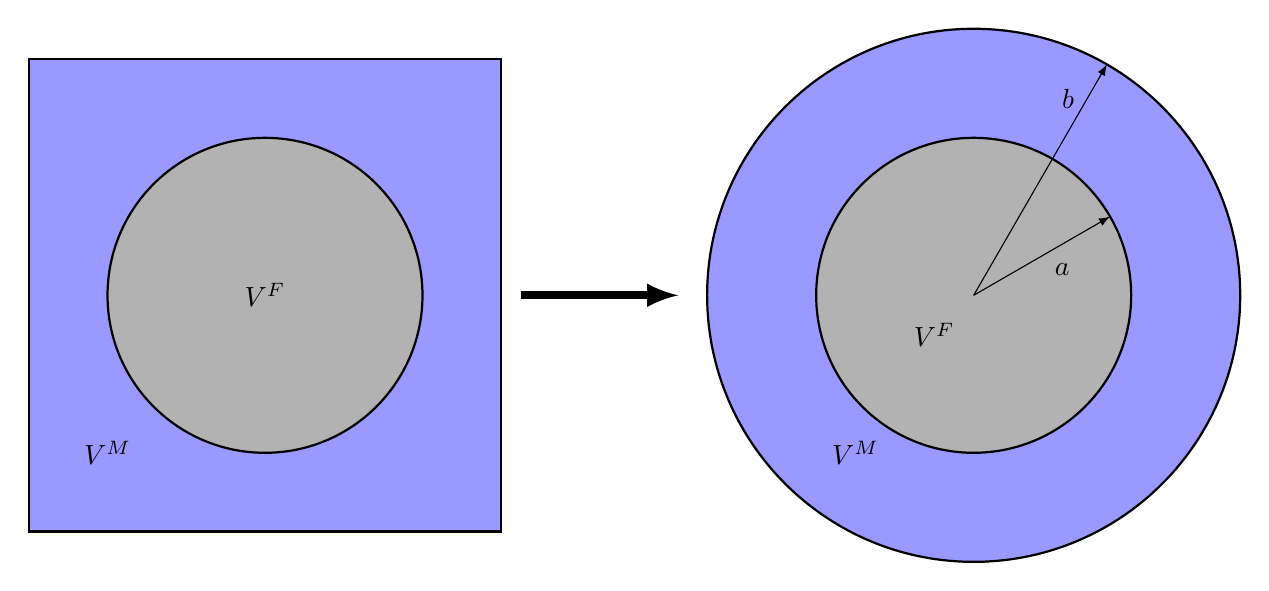
\begin{tikzpicture}
  \filldraw[blue!40] (0,0) -- (0,6) -- (6,6) -- (6,0) -- cycle;
  \filldraw[gray!60] (3,3) circle (2cm);
  \draw[thick] (3,3) circle (2cm);
  \draw[thick] (0,0) -- (0,6) -- (6,6) -- (6,0) -- cycle;
  \node at (3,3) {$V^F$};
  \node at (1,1) {$V^M$};
  
  \draw[line width=1mm,-latex] (6.25,3) -- (8.25,3);
  
  \filldraw[blue!40] (12,3) circle (3.385cm);
  \filldraw[gray!60] (12,3) circle (2cm);
  \draw[thick] (12,3) circle (2cm);
  \draw[thick] (12,3) circle (3.385cm);
  \draw[-latex] (12,3) -- (13.732,4);
  \draw[-latex] (12,3) -- (13.6925,5.932);
  \node at (11.5,2.5) {$V^F$};
  \node at (10.5,1) {$V^M$}; 
  \node at (13.125,3.325) {$a$};
  \node at (13.2,5.5) {$b$};
\end{tikzpicture}
\end{center}
\caption{Equivalent annular unit cell with an equal volume moderator}
\label{Fig:thermalization_cylindricizedUnitCell}
\end{center}
\end{figure}

With all this background discussion, we begin the ABH method. The first step is to take the unit cell and approximate the moderator as an annular region that has an equal volume as the actual unit cell. This process is called cylindricization and depicted in Fig.~\ref{Fig:thermalization_cylindricizedUnitCell}. (The ABH method can also be applied to spherical fuel elements and the unit cell box is made into an equivalent volume spherical shell.) Here we take $a$ to the radius of the fuel and $b$ to be the radius of the annular moderator.

The next step is to solve a neutron diffusion problem within the annular moderator region. The problem statement is as follows:
\begin{subequations}
\begin{align}
  &\frac{1}{r} \frac{d}{dr} \left( r \frac{d\phi^M}{dr} \right) - \frac{1}{L_M^2} \phi^M(r) = -\frac{1}{\pi D^M (b^2 - a^2)} , \quad a \le r \le b, \\*
  &\phi(a-\delta) = 0, \\*
  &J(b) = 0.
\end{align}
\end{subequations}
Here $\delta$ is the extrapolation distance, for which we can use the Milne extrapolation of $0.7104/\Sigma_{tr}$. The other quantities $D^M$ and $L^M$ are the diffusion coefficient and diffusion length of the moderator and follow the same definitions as for all one-speed neutron diffusion problems. Note the volume of the moderator is $V^M = \pi ( b^2 - a^2 )$ and the internal source is normalized to unity. The form of the solution is in terms of modified Bessel functions and becomes a bit of a mess. Given this solution $\phi^M(r)$, we can solve for the the moderator escape probability as one minus the absorption probability,
\begin{align}
  p_{esc}^M = 1 - 2\pi \int_a^b \Sigma_a^M \phi^M(r) r dr .
\end{align}
(This result is a probability because the source is of unit intensity.) The full form of the reciprocal of the moderator escape probability is (after a lot of algebra),
\begin{align}
 \frac{1}{p_{esc}^M} = \frac{\delta}{4 D^M} \Sigma_a^M \overline{s}^M + F,
\end{align}
where $F$ is some geometrical factor, which for cylindrical geometry is
\begin{align}
  F = \frac{ (b/L^M)^2 - (a/L^M)^2 }{ 2 a/L^M } \frac{ I_0(a/L^M) K_1(b/L^M) + K_0(a/L^M) I_1(b/L^M) }{ I_1(b/L^M) K_1(a/L^M) - K_1(b/L^M) I_1(a/L^M) } .
\end{align}
If we were to solve the ABH method in slab or spherical geometry, the reciprocal of the escape probability would take the same general form, but with a different factor $F$.

We have the escape probability in the moderator by solving a diffusion problem and can get the escape probability in the fuel using Eq.~\eqref{Eq:thermalization_escapeProbability_CollisionProbabilityMethod}. The next step is to stitch these together in away that we can extract the thermal disadvantage factor from Eq.~\eqref{Eq:thermalization_disadvantageFactor}. The process is to write four well-chosen balance relationships that with the blackness identities for the fuel and moderator regions, can be manipulated to obtain an expression for the thermal disadvantage factor. Prior to doing this, we define:
\begin{align}
  Q &= \frac{1}{\pi (b^2 - a^2)} = \text{ uniform slowing down source in the moderator}, \nonumber \\
  J_{F \rightarrow M} &= \text{ partial current of neutrons entering the fuel from the moderator}, \nonumber \\
  J_{M \rightarrow F} &= \text{ partial current of neutrons entering the moderator from the fuel}. \nonumber
\end{align}
The specific value of $Q$ naturally differs if we solve the problem is slab or spherical geometries instead of cylindrical.

\begin{subequations}
The first balance relationship pertains to the absorptions within the moderator:
\begin{align}
  \underbrace{\Sigma_a^M \overline{\phi}^M V^M}_{\parbox{2cm}{\scriptsize absorption rate in the moderator}}
  = \underbrace{Q V^M ( 1 - p_{esc}^M )}_{\parbox{3cm}{\scriptsize absorption rate from neutrons that thermalize never enter the fuel}}
  + \underbrace{J_{F \rightarrow M} S \beta^M}_{\parbox{3cm}{\scriptsize absorption rate from neutrons that return after being in the fuel}}.
\end{align}
The second balance relationship gives the accounting of absorptions within the fuel:
\begin{align}
  \underbrace{\Sigma_a^F \overline{\phi}^F V^F}_{\parbox{2cm}{\scriptsize absorption rate in the fuel}}
  = \underbrace{J_{M \rightarrow F} S \beta^F}_{\parbox{3cm}{\scriptsize absorption rate from neutrons that enter the fuel from moderator}}.
\end{align}
The third balance relationship is over the entire unit cell:
\begin{align}
  \underbrace{\Sigma_a^M \overline{\phi}^M V^M}_{\parbox{2cm}{\scriptsize absorption rate in the moderator}}
  + \underbrace{\Sigma_a^F \overline{\phi}^F V^F}_{\parbox{2cm}{\scriptsize absorption rate in the fuel}}
  = \underbrace{Q V^M}_{\parbox{2cm}{\scriptsize rate neutrons thermalize in the moderator}}.
\end{align}
The final balance relationship is a statement that when a neutron enters the fuel it must either be absorbed or leak back out:
\begin{align}
  \underbrace{\beta^F}_{\parbox{2cm}{\scriptsize probability that a neutron entering fuel is absorbed before leaking back out}}
  + \underbrace{\frac{ J_{F \rightarrow M} }{ J_{M \rightarrow F} }}_{\parbox{2cm}{\scriptsize probability that a neutron entering fuel is leaks out before being absorbed}}
  = 1.
\end{align}
Finally, we write down the blackness identities for the fuel and moderator, repsectively:
\begin{align}
  p_{esc}^F &= \Sigma_a^F \overline{s}^F \beta^F, \\
  p_{esc}^M &= \Sigma_a^M \overline{s}^M \beta^M.
\end{align}
\end{subequations}

These six equations can then be used to obtain an expression for the ratio of the thermal disadvantage factor:
\begin{align}
  \zeta = \frac{1}{p_{esc}^F} + \frac{ \Sigma_a^F \overline{s}^F }{ \Sigma_a^M \overline{s}^M } \left( \frac{1}{p_{esc}^M} - \Sigma_a^M \overline{s}^M - 1  \right) .
\end{align}
This disadvantage factor may then be used to compute the flux-weighted thermal group cross sections.

\subsection{Escape Cross Section and Dancoff Factor}

The ABH method works reasonably well for predicting the flux-weighted thermal group cross section. Unfortunately, such a treatment is invalid for fast neutrons and therefore cannot be used to predict the resonance integrals to calculate the fast group cross sections. The reason is a typical fast neutron has a mean-free path that is much greater than the unit cell, where a typical neutron may traverse several of them in a single flight. Also, in resonances, the fuel is essentially opaque to the neutrons. This means that diffusion theory is entirely inadequate and we either need to use a transport calculation or some other scheme.

First, we revisit the first-flight escape probability $p_{fm}$. This was derived under the assumption that when a neutron leaks out, it goes into the moderator and is effectively guaranteed to collide in the moderator because of its optical thickness. This is equivalent to treating the fuel as being surrounded by an effectively infinite moderator.

In other words, we neglected entirely the possibility that a neutron escapes the fuel and collides in a \emph{different} fuel element in the lattice. In the unit cell model, we use reflecting boundary conditions to simulate the lattice and a fast neutron often bounce off the edge of the unit cell multiple times before experiences a collision. The first-flight escape probability we  currently have can be approximated using the Wigner rational approximation in Eq.~\eqref{Eq:thermalizaiton_WignerRationalApproximation}. We can write this slightly by dividing both the numerator and denominator by the mean chord length of the fuel,
\begin{align}
  p_{fm}(E) = \frac{ \frac{1}{\overline{s}^F} }{ \frac{1}{\overline{s}^F} + \Sigma_t^F(E) } .
\end{align}

This seemingly trivial rearrangement yields something interesting. The inverse mean chord length is the numerator and appears in the denominator. Since this quantity describes a neutron escaping the fuel, we can think of this as a pseudo cross section called the \emph{escape cross section} for the fuel not counting collisions in other fuel elements. We can write this equivalently as
\begin{align}
  \frac{1}{\overline{s}^F}
  = &\text{ escape ``cross section'' of the fuel} \nonumber \\
  = &\text{ probability per unit length of an average neutron leaking out of the fuel} \nonumber \\*
    &\text{ and colliding in the moderator that has infinite optical thickness.} \nonumber
\end{align}
Specifying that the moderator has infinite optical thickness means that 

Of course, the moderator does not have infinite optical thickness nor is it even a reasonable approximation for fast neutrons. We can try to drop the caveat of an infinite moderator by reducing the escape cross section to not count collisions in another fuel element as an escape. This is done through a correction factor that we refer to as the \emph{Dancoff correction factor}. This is defined as
\begin{align}
  C = &\text{ the probability that a neutron that has just leaked out of a fuel element} \nonumber \\*
      &\text{ undergoes its next collision in a different fuel element.} \nonumber
\end{align}
Therefore, the compliment of the Dancoff factor is
\begin{align}
  1 - C = 
  &\text{ the probability that a neutron that has just leaked out of a fuel element} \nonumber \\*
  &\text{ undergoes its next collision in the moderator.} \nonumber
\end{align}
Therefore, the product of these may be used to define a \emph{reduced escape cross section} for the fuel
\begin{align}
  \Sigma_e^F = &\ N^F \sigma_e^F = (1 - C) \frac{1}{\overline{s}^F} \\
  = &\text{ ( probability per unit length of an average neutron leaking out of the fuel )} \nonumber \\*
  \times    &\text{ ( the probability that a neutron that has just leaked out of a fuel element} \nonumber \\*
  &\text{ undergoes its next collision in the moderator )} \nonumber \\
  = &\text{ probability per unit length of an average neutron leaking out of the fuel } \nonumber \\* 
  &\text{ and colliding in the moderator.} \nonumber
\end{align}
In the limiting case where the moderator has an infinite optical thickness, the neutrons cannot interact with any other fuel element. Note that the Dancoff factor and reduced escape cross section is, in general, energy dependent because it depends on the material properties of both the moderator and the fuel. For the case of optically thick fuel, almost all neutrons are absorbed almost immediately upon entering the fuel and the cross sections are fairly independent of energy in the slowing down range, so we often can take the escape cross section as not a strong function of energy.

Given this, we can correct the escape cross section to obtain the first-flight collision probability for the fuel into the moderator:
\begin{align}
  p_{FM}(E) &= \ \frac{ (1 - C) \frac{1}{\overline{s}^F} }{ (1 - C) \frac{1}{\overline{s}^F}+ \Sigma_t^F(E) } = \frac{ \sigma_e^F }{ \sigma_e^F + \sigma_t^F(E) } \label{Eq:thermalization_wignerRationalApproximation_pFM} \\
  &= \text{ the probability that a neutron leaks out of the fuel and experiences its } \nonumber \\*
  &\quad \ \text{ next collision in the moderator.} \nonumber
\end{align}
Here the capital letters distinguish this probability for the entire lattice from the first-flight probability for a single fuel element. We can also define the same for the moderator:
\begin{align}
  p_{MF}(E) 
  &= \text{ the probability that a neutron leaks out of the moderator and experiences } \nonumber \\*
  &\quad \ \text{ its next collision in the fuel.} \nonumber
\end{align}

The natural question then is how we calculate the Dancoff factor $C$. Unfortunately, with the exception of slab geometry, there is no closed form solution and most often we have to rely on computational methods involving ray tracing with Monte Carlo methods. The idea is to randomly sample neutrons uniformly on the fuel-moderator interface $S$ along with a random direction distributed as an isotropic angular flux or cosine source. We then sample the number of mean-free paths that the neutron samples from an exponential distribution and then determine whether or not the neutron collides in a fuel element. If it does, we count that as a success. We then repeat this process a large number of times and estimate the Dancoff correction factor by taking the ratio of the number of successes to the number of rays cast.

There is an alternative way that works reasonably well for the case of the fuel being optically thick such that a neutron is effectively guaranteed to collide within the a fuel if it reaches it, which is reasonable if the neutron energy corresponds to a resonance energy where we most want to compute it. When this is the case, we can use a first-order Taylor series to estimate the expected probability of a random neutron leaking out of the fuel reaching another fuel element. This is
\begin{align}
  C \approx e^{-\Sigma_t^M \overline{s}^M} , \quad \Sigma_t^{F} \overline{s}^F \gg 1.
\end{align}

Before leaving the topic, we should comment that we now have two effective leakage cross sections. In diffusion theory, we have the effective leakage cross section as $B^2 D$, which of course assumes that diffusion theory is valid. This alternative escape cross section also describes leakage, but for the case that the region is non-diffusive, experiencing few scatters and thereby not changing direction within the region on its flight. The escape cross section is inversely proportional to the mean chord length and therefore inversely proportional to the region volume, which makes sense because we expect a geometrically smaller system to be more leaky. So the short answer is we use $B^2 D$ in diffusive scenarios and $1/\overline{s}$ in streaming dominated ones.

\subsection{First-Flight Collision Equations for Fast Neutrons}

The next step to describing fast neutrons so we can compute resonance integrals is writing down balance relationships in terms of the first-flight collision probabilities $p_{FM}$ and $p_{MF}$. The goal is to formulate two transport problems that we can use to determine the two unknown region-averaged scalar fluxes in the fuel and moderator. In this spirit, we can also use the reciprocity relationship to obtain a relationship between $p_{FM}$ and $p_{MF}$, where the former can be estimated using the Wigner rational approximation with the Dancoff factor corrections.

The first step is to take the steady-state neutron transport equation assuming isotropic scattering:
\begin{align}
  \dir \cdot \nabla \psi(\pos,\dir,E) + \Sigma_t(\pos,E) \psi(\pos,\dir,E) = \frac{1}{4\pi} q_s(\pos,\dir,E),
\end{align}
where $q(\pos,\dir,E)$ describes the scattering sources,
\begin{align}
  q_s(\pos,\dir,E) = \left\{ \begin{array}{l l}
  \displaystyle\int_E^{E/\alpha^F} \dfrac{ \Sigma_s^F(E') }{ 1 - \alpha^F } \psi(\pos,\dir,E') \dfrac{ dE' }{ E' } , & \quad \pos \in R^F, \\
  \displaystyle\int_E^{E/\alpha^M} \dfrac{ \Sigma_s^M(E') }{ 1 - \alpha^M } \psi(\pos,\dir,E') \dfrac{ dE' }{ E' } , & \quad \pos \in R^M. \\ \end{array} \right. 
\end{align}
The boundary conditions at the edges of the unit cell are reflecting. Per earlier definitions, $\alpha^{F/M}$ are the scattering parameters for the fuel and moderator. In this, description we are assuming a single isotope per region. We could add more isotopes and still get to a solution, but it would complicate the problem by having more integrals in the scattering sources. 

To obtain two equations, we integrate the neutron transport equation over the two spatial regions. The first equation is obtained by integrating over the fuel region $R^F$ and all directions to obtain a neutron continuity equation for the fuel. We also write the solution in terms of the volume-averaged scalar flux in the fuel $\overline{\phi}^F$, but this still leaves the current vector $\mathbf{J}$ from the streaming term. We then apply the divergence theorem to convert the volume integral over the streaming term or current vector into a surface integral. After these steps we obtain
\begin{subequations} 
\begin{align}
  &J_{F \rightarrow M }(E) + \Sigma_t^F(E) V^F \overline{\phi}^F(E) \nonumber \\*
  &= \displaystyle\int_E^{E/\alpha^F} \dfrac{ \Sigma_s^F(E') V^F }{ 1 - \alpha^F } \overline{\phi}^F(\pos,\dir,E') \dfrac{ dE' }{ E' }. \label{Eq:thermalization_flatSourceEquationFuel_step1}
\end{align}
We get a second equation by doing the same except integrating over the moderator region $R^M$, giving
\begin{align}
  &-J_{F \rightarrow M }(E) + \Sigma_t^M(E) V^M \overline{\phi}^M(E) \nonumber \\*
  &= \displaystyle\int_E^{E/\alpha^F} \dfrac{ \Sigma_s^M(E') V^M }{ 1 - \alpha^F } \overline{\phi}^M(\pos,\dir,E') \dfrac{ dE' }{ E' }. \label{Eq:thermalization_flatSourceEquationModerator_step1}
\end{align}
where
\begin{align}
  J_{F \rightarrow M }(E)
  &= \int_{4\pi} \int_S ( \dir \cdot \nhat^F ) \psi(\pos,\dir,E) dA d\Omega \nonumber \\
  &= \int_S \nhat^F \cdot \mathbf{J}(\pos,E) dA \label{Eq:thermalization_flatSource_netCurrent}
\end{align}
\end{subequations}
that is the net current flowing out from the fuel into the moderator. For this we note the outward unit normal vector of the moderator is aligned in the opposite direction of the fuel, hence the minus sign on the net current in the second equation. By inspecting these two equations, we are back to the scenario of having more unknowns ($\overline{\phi}^F, \overline{\phi}^F$, and $J_{F \rightarrow M }$) than equations.

The first step to closing these equations is to approximate the angular flux to compute the net current. First, we assume a spatially flat, isotropic scattering source within each region with the magnitude given by the respective volume-averaged scalar fluxes, but allow the neutron angular flux to vary. Normally the scattering source varies continuously with position as described by the angular flux. Specifically, the internal source in this transport problem is
\begin{align}
  Q(\pos,\dir,E) = \left\{ \begin{array}{l l}
  \dfrac{1}{4\pi} \overline{Q}^F(E), & \quad \pos \in R^F; \quad \pos \in S, \nhat^F \cdot \dir > 0, \vspace{0.2cm} \\ 
  \dfrac{1}{4\pi} \overline{Q}^M(E), & \quad \pos \in R^M; \quad \pos \in S, \nhat^F \cdot \dir < 0. \\ \end{array} \right.
\end{align}
where
\begin{subequations} \label{Eq:thermalization_flatScatteringSources_Qbar}
\begin{align}
  \overline{Q}^F(E) &= \displaystyle\int_E^{E/\alpha^F} \dfrac{ \Sigma_s^F(E') }{ 1 - \alpha^F } \dfrac{ \overline{\phi}^F(E') }{ E' } dE', \\
  \overline{Q}^M(E) &= \displaystyle\int_E^{E/\alpha^M} \dfrac{ \Sigma_s^M(E') }{ 1 - \alpha^M } \dfrac{ \overline{\phi}^M(E') }{ E' } dE'.
\end{align}
\end{subequations}
It is important to note how the source is defined on the fuel-moderator interface $S$. On this boundary, we use $\overline{Q}^F(E)$ for directions leaving the fuel and $\overline{Q}^M(E)$ for directions entering the fuel.

We now write the neutron transport equation over the unit cell with a spatially flat source as
\begin{align}
  \dir \cdot \nabla \psi_{fs}(\pos,\dir,E) + \Sigma_t(\pos,E) \psi_{fs}(\pos,\dir,E) = Q(\pos,\dir,E). \label{Eq:thermalization_flatSourceEquation_initialForm}
\end{align}
We refer to this form of the neutron transport problem as the \emph{flat source equation}. Because we assume a spatially flat scattering source, the angular flux does not explicitly appear on the right hand side; it is implicit via the volume-averaged scalar flux, but this still helps matters considerably.

Next, we formulate two transport problems defined over the entire unit cell such that their linear combination gives the flat source equation. The first problem we denote with a superscript $F$ such that we have a uniform, isotropic, unit source in the fuel. This is
\begin{subequations}
\begin{align}
  \dir \cdot \nabla \psi^F(\pos,\dir,E) + \Sigma_t(\pos,E) \psi^F(\pos,\dir,E) = 
  \left\{ \begin{array}{l l} 
  \dfrac{1}{4\pi V^F}, & \quad \pos \in R^F, \\
  0, & \quad \pos \in R^M. \\ \end{array} \right. \label{Eq:thermalization_flatSource_psiF}
\end{align}
The second transport problem has a superscript $M$ and has a uniform isotropic source within the moderator:
\begin{align}
  \dir \cdot \nabla \psi^M(\pos,\dir,E) + \Sigma_t(\pos,E) \psi^M(\pos,\dir,E) = 
  \left\{ \begin{array}{l l} 
  0, & \quad \pos \in R^F, \\
  \dfrac{1}{4\pi V^M}, & \quad \pos \in R^M. \\ \end{array} \right. \label{Eq:thermalization_flatSource_psiM}
\end{align}
\end{subequations}
An important feature of both of these problems is they do not involve scattering. This means they fall into a class of problems called purely absorbing, which are much easier to solve.

If we inspect the two problems for $\psi^F$ and $\psi^M$ and compare it with the form of the original neutron transport problem in Eq.~\eqref{Eq:thermalization_flatSourceEquation_initialForm}, we can deduce what linear combination of $\psi^F$ and $\psi^M$ gives that equation. This is
\begin{align}
  \psi_{fs}(\pos,\dir,E) = V^F \overline{Q}^F(E) \psi^F(\pos,\dir,E) + V^M \overline{Q}^M(E) \psi^M(\pos,\dir,E) . \label{Eq:thermalization_flatSourceAngularFlux}
\end{align}
We can show this is right by multiplying Eq.~\eqref{Eq:thermalization_flatSource_psiF} by $V^F \overline{Q}^F(E)$, Eq.~\eqref{Eq:thermalization_flatSource_psiM} by $V^M \overline{Q}^M(E)$, and adding them together.

Another very important feature of these two transport problems is that because of how the sources in each problem are defined, we can relate $\psi^F$ and $\psi^M$ to the first-flight collision probabilities. These are
\begin{subequations} \label{Eq:thermalization_pFM_pMF_flatSource_collisionIntegral}
\begin{align}
  p_{FM}(E) &= \int_{4\pi} \int_{R^M} \Sigma_t^M \psi^F(\pos,\dir,E) dV d\Omega, \label{Eq:thermalization_pFM_flatSource_collisionIntegral} \\
  p_{MF}(E) &= \int_{4\pi} \int_{R^F} \Sigma_t^F \psi^M(\pos,\dir,E) dV d\Omega. \label{Eq:thermalization_pMF_flatSource_collisionIntegral}
\end{align}
\end{subequations}
So for $p_{FM}$, we use $\psi^F$ because the source is uniformly and isotropically within the fuel and we find the collision rate in the moderator by integrating over the moderator volume and all directions. The case is similar for $p_{MF}$, except the role of fuel and moderator are reversed. 

Based on these definitions, we can relate these probabilities to the net currents. To see this, we integrate Eq.~\eqref{Eq:thermalization_flatSource_psiF} for $\psi^F$ over the moderator $R^M$ and all directions. After applying the divergence theorem to convert the volume integral into a surface integral, we get
\begin{align}
  &-\int_{4\pi} \int_S \nhat^F \cdot \dir \psi^F(\pos,\dir,E) dA d\Omega + \int_{4\pi} \int_{R^M} \Sigma_t^M(E) \psi^F(\pos,\dir,E) dV d\Omega = 0. 
\end{align}
By Eq.~\eqref{Eq:thermalization_pFM_flatSource_collisionIntegral}, we see that the second term is $p_{FM}$. The right-hand side is zero because the source is in the fuel and we integrated over the moderator. Therefore, the first-flight collision probability is
\begin{subequations}
\begin{align}
  p_{FM}(E) = \int_{4\pi} \int_S \nhat^F \cdot \dir \psi^F(\pos,\dir,E) dA d\Omega  . 
\end{align}
Similarly, integrating Eq.~\eqref{Eq:thermalization_flatSource_psiM} for $\psi^M$ over the fuel $R^F$ and all directions and then going through the same reasoning, we get
\begin{align}
  p_{MF}(E) = -\int_{4\pi} \int_S \nhat^F \cdot \dir \psi^M(\pos,\dir,E) dA d\Omega . 
\end{align}
\end{subequations}
Again, the minus sign arises because the unit normal for flow out of the fuel or moderator point in opposite directions.

We now use $\psi_{fs}$ to approximate the net current $J_{F \rightarrow M}$. We insert this angular flux from Eq.~\eqref{Eq:thermalization_flatSourceAngularFlux} into equation into Eq.~\eqref{Eq:thermalization_flatSource_netCurrent} and write the result in terms of the first-flight collision probabilities:
\begin{align}
  J_{F \rightarrow M }
  &= \int_{4\pi} \int_S ( \nhat^F \cdot \dir ) \psi_{fs}(\pos,\dir,E) dA d\Omega \nonumber \\
  &= \int_{4\pi} \int_S ( \nhat^F \cdot \dir ) \left[ V^F \overline{Q}^F(E) \psi^F(\pos,\dir,E) + V^M \overline{Q}^M(E) \psi^M(\pos,\dir,E)  \right] dA d\Omega \nonumber \\
  &= V^F \overline{Q}^F(E) \int_{4\pi} \int_S ( \nhat^F \cdot \dir )  \psi^F(\pos,\dir,E)  dA d\Omega \nonumber \\*
  &+ V^M \overline{Q}^M(E) \int_{4\pi} \int_S  ( \nhat^F \cdot \dir ) \psi^M(\pos,\dir,E)  dA d\Omega \nonumber \\
  &= V^F \overline{Q}^F(E) p_{FM}(E) - V^M \overline{Q}^M(E) p_{MF}(E) .
\end{align}
Now that we have the net currents, we can substitute this into Eqs.~\eqref{Eq:thermalization_flatSourceEquationFuel_step1} and~\eqref{Eq:thermalization_flatSourceEquationModerator_step1}. This yields the following balance relation on first-flight collisions:
\begin{subequations}
\begin{align}
     \underbrace{V^F \overline{Q}^F(E) p_{FM}(E)}_{\parbox{3cm}{\scriptsize rate neutrons born in fuel are removed by streaming into and colliding in moderator}}
   + \underbrace{V^F  \Sigma_t^F(E) \overline{\phi}^F(E)}_{\parbox{2.75cm}{\scriptsize rate neutrons are removed by colliding in fuel}}
   = \underbrace{V^F \overline{Q}^F(E)}_{\parbox{2cm}{\scriptsize rate neutrons are scattered into energy $E$ in fuel}}
   + \underbrace{V^M \overline{Q}^M(E) p_{MF}(E)}_{\parbox{3cm}{\scriptsize rate neutrons are scattered into energy $E$ in moderator and then stream into and collide in fuel}}, \label{Eq:thermalization_flatSourceEquation_fuel} \\
%%%%%
     \underbrace{V^M \overline{Q}^M(E) p_{MF}(E)}_{\parbox{3cm}{\scriptsize rate neutrons born in moderator are removed by streaming into and colliding in fuel}}
   + \underbrace{V^M  \Sigma_t^M(E) \overline{\phi}^F(E)}_{\parbox{2.75cm}{\scriptsize rate neutrons are removed by colliding in moderator}}
   = \underbrace{V^M \overline{Q}^M(E)}_{\parbox{2cm}{\scriptsize rate neutrons are scattered into energy $E$ in moderator}}
   + \underbrace{V^F \overline{Q}^F(E) p_{FM}(E)}_{\parbox{3cm}{\scriptsize rate neutrons are scattered into energy $E$ in fuel and then stream into and collide in moderator}}. \label{Eq:thermalization_flatSourceEquation_moderator}
\end{align}
\end{subequations}
While these equations look very elegant, we still have more unknowns (apparently four now: $\overline{\phi}^F, \overline{\phi}^M, p_{FM}$, and $p_{MF}$) than equations, these two plus the Wigner rational approximation to estimate $p_{FM}$, provided we have a way to estimate the Dancoff factor or escape cross section. So we are still left with needing one additional relationships, which we do next.

\subsection{First-Flight Collision Reciprocity Relationship}

The resolution of this involves using the transport problems for $\psi^F$ and $\psi^M$ and applying the reciprocity theorem in Eq.~\eqref{Eq:thermalization_generalizedReciprocityTheorem} to relate $p_{FM}$ and $p_{MF}$. In this we let transport 1 be that for $\psi^F$ and transport problem 2 be that for $\psi^M$. Inserting these into the reciprocity theorem, we have
\begin{align}
  \int_{4\pi} \int_R  \psi^M(\pos,-\dir,E) \frac{1}{4\pi V^F} - \psi^F(\pos,\dir,E) \frac{1}{4\pi V^M} dV d\Omega = 0.
\end{align}
(Note the fact that the reciprocity theorem we derived not including energy dependence here does not impact anything because these problems are purely absorbing and have no mechanism for changing energy.) 

We can flip $-\dir$ to $\dir$ on the angular flux in the first term without consequence since it is the only thing on that term that depends on direction and we are integrating over all directions. We then multiply and divide the first term by $\Sigma_t^F$ and do the same for the second term, but with $\Sigma_t^M$. After moving the second term to the right and side, we get
\begin{align}
  V^M \Sigma_t^M \int_{4\pi} \int_R \Sigma_t^F \psi^M(\pos,\dir,E) dV d\Omega  = V^F \Sigma_t^F \int_{4\pi} \int_R \Sigma_t^M \psi^F(\pos,\dir,E)  dV d\Omega .
\end{align}

Then, we simply apply Eq.~\eqref{Eq:thermalization_pFM_pMF_flatSource_collisionIntegral} to write the integrals in terms of the first-flight collision probabilities and obtain the result:
\begin{align}
  V^M \Sigma_t^M(E)  p_{MF}(E)  = V^F \Sigma_t^F(E) p_{FM}(E). \label{Eq:thermalization_firstFlightCollisionReciprocityRelationship}
\end{align}
This is called the \emph{first-flight collision reciprocity relationship} or sometimes (confusingly) just the reciprocity relationship. We now have four equations: the two first-flight collision equations, the Winger rational approximation, and this new relationship. This is sufficient to apply the same resonance approximations we used for a homogeneous mixture to obtain resonance integrals. 

\subsection{Resonance Integrals and the Equivalence Relationship}

To compute the resonance integrals, we first take the flat source equation for the fuel, Eq.~\eqref{Eq:thermalization_flatSourceEquation_fuel}, and bring all the scattering terms to the right-hand side:
\begin{align}
   V^F \Sigma_t^F(E) \overline{\phi}^F(E) = [ 1 - p_{FM}(E) ] V^F \overline{Q}^F(E) + p_{MF}(E) V^M \overline{Q}^M(E) .
\end{align}
Recall that the sources $\overline{Q}^F(E)$ and $\overline{Q}^M(E)$ are integrals from Eq.~\eqref{Eq:thermalization_flatScatteringSources_Qbar},
\begin{align}
  \overline{Q}^F(E) &= \displaystyle\int_E^{E/\alpha^F} \dfrac{ \Sigma_s^F(E') }{ 1 - \alpha^F } \dfrac{ \overline{\phi}^F(E') }{ E' } dE', \nonumber \\ 
  \overline{Q}^M(E) &= \displaystyle\int_E^{E/\alpha^M} \dfrac{ \Sigma_s^M(E') }{ 1 - \alpha^M } \dfrac{ \overline{\phi}^M(E') }{ E' } dE'. \nonumber
\end{align}
To get rid of these integrals, we can apply one of the approximations we used for the homogeneous mixture. If we use the NR approximation (see Sec.~\ref{Sec:thermalization_narrowResonanceApproximation_HomogeneousMixture}), we get that
\begin{subequations}
\begin{align}
  \overline{Q}_{NR}^F(E) &= \frac{\Sigma_p^F}{E}, \\
  \overline{Q}_{NR}^M(E) &= \frac{\Sigma_s^M}{E}.
\end{align}
\end{subequations}

Inserting these into the flat source equation and dividing by the volume gives
\begin{align}
   \Sigma_t^F(E) \overline{\phi}^F_{NR}(E) = [ 1 - p_{FM}(E) ]  \frac{\Sigma_p^F}{E} + \frac{V^M}{V^F} p_{MF}(E) \frac{\Sigma_s^M}{E}.
\end{align}
However, from the first-flight collision reciprocity relationship, Eq.~\eqref{Eq:thermalization_firstFlightCollisionReciprocityRelationship}, we have
\begin{align}
  \frac{V^M}{V^F} p_{MF}(E) = \frac{\Sigma_t^F}{\Sigma_t^M} p_{FM}(E) = \frac{\Sigma_t^F}{\Sigma_s^M} p_{FM}(E) . \nonumber
\end{align}
(Here we note that absorption of fast neutrons in the moderator is negligible.) Inserting this and dividing by the total cross section, we obtain
\begin{align}
  \overline{\phi}^F_{NR}(E) 
  &= \frac{ [ 1 - p_{FM}(E) ] \Sigma_p^F + \Sigma_t^F p_{FM}(E) }{ \Sigma_t^F(E) } \frac{1}{E} \nonumber \\
  &= \frac{ \Sigma_p^F + [ \Sigma_{rs}^F(E) + \Sigma_a^F(E) ] p_{FM}(E) }{ \Sigma_t^F(E) } \frac{1}{E} \nonumber \\
  &= \frac{ \sigma_p^F + [ \sigma_{rs}^F(E) + \sigma_a^F(E) ] p_{FM}(E) }{ \sigma_t^F(E) } \frac{1}{E} .
\end{align}
We are able to convert to microscopic cross sections because all the cross sections are for the fuel.

Next, we apply the Wigner rational approximation with the reduced escape cross section, Eq.~\eqref{Eq:thermalization_wignerRationalApproximation_pFM} to approximate the first-flight collision probability
\begin{align}
  p_{FM}(E) \approx \frac{ \sigma_e^F }{ \sigma_e^F + \sigma_t^F(E) } . \nonumber
\end{align}
Inserting this into the expression for the volume-averaged scalar flux and multiplying both the numerator and denominator by $\sigma_e^F + \sigma_t^F(E)$, we get
\begin{align}
  \overline{\phi}^F_{NR}(E) 
  &= \frac{ \sigma_p^F [ \sigma_e^F + \sigma_t^F(E) ]  + [ \sigma_{rs}^F(E) + \sigma_a^F(E) ] \sigma_e^F }{ [ \sigma_e^F + \sigma_t^F(E) ] \sigma_t^F(E)  } \frac{1}{E}  \nonumber \\
  &= \frac{ \sigma_e^F [ \sigma_p^F + \sigma_{rs}^F(E) + \sigma_a^F(E) ] + \sigma_p^F \sigma_t^F(E) }{ [ \sigma_e^F + \sigma_t^F(E) ] \sigma_t^F(E)  } \frac{1}{E} . \nonumber
\end{align}
Notice after some rearrangement there is a common factor of $\sigma_t^F(E) = \sigma_p^F + \sigma_{rs}^F(E) + \sigma_a^F(E)$ on each term in the numerator and the denominator. After canceling these, and expanding out the total cross section in the denominator, we have the result for the NR approximation:
\begin{align}
  \overline{\phi}^F_{NR}(E) 
  &= \frac{ \sigma_e^F + \sigma_p^F }{ \sigma_e^F + \sigma_p^F  + \sigma_{rs}^F(E) + \sigma_a^F(E) } \frac{1}{E} . \label{Eq:thermalization_flatSourceScalarFlux_NR}
\end{align}

The resonance integral is
\begin{align}
  I_j^{NR} = \int_{\Delta E_{rj}} \sigma_a^F(E) \overline{\phi}^F_{NR}(E) dE.
\end{align}
Inserting the volume-averaged scalar flux for the fuel in Eq.~\eqref{Eq:thermalization_flatSourceScalarFlux_NR} and noting that $1/E$ varies slowing with respect to the rest of the integrand over the narrow range of the resonance, we have
\begin{align}
  I_j^{NR} = \frac{\sigma_e^F + \sigma_p^F}{E_{rj}} \int_{\Delta E_{rj}} \frac{ \sigma_a^F(E) }{ \sigma_e^F + \sigma_p^F + \sigma_{rs}^F(E) + \sigma_a^F(E) } dE. \label{Eq:thermalization_resonanceIntegral_NR_flatSource}
\end{align}

This result looks very similar to the homogeneous case. If we inspect Eq.~\eqref{Eq:thermalization_resonanceIntegral_NR_expandedForm}, we can deduce that the equivalent resonance integral is
\begin{align}
  I_{j,hom}^{NR} &= \frac{(N^M V^M)/(N^F V^F) \sigma_s^M + \sigma_p^F }{E_{rj}} \nonumber \\
  &\times \int_{\Delta E_{rj}} \frac{ \sigma_a^F(E)  }{ (N^M V^M)/(N^F V^F) \sigma_s^M + \sigma_p^F + \sigma_{rs}^F(E) + \sigma_a^F(E) } dE . 
\end{align}
Note the extra volume weighting of the number densities is because to create an equivalent homogeneous mixture, we need to mix the fuel and moderator materials, which to be consistent with the heterogeneous lattice, have respective atomic densities $N^F$ and $N^M$. 

In comparing the two resonance integrals only difference here is that instead of having $(N^M V^M)/(N^F V^F) \sigma_s^M$ in the homogeneous case, we have the escape cross section $\sigma_e^F$ for the lumped model. This is actually an important point and we call this an \emph{equivalence relationship} for the resonance integral. There are two consequences:
\begin{enumerate}
  \item An infinite lattice using the lumped model (with the escape cross section the Wigner rational approximation) with a reduced escape cross section $\sigma_e^F$ has the same resonance integral as a homogeneous mixture with the equivalent value of $(N^M V^M)/(N^F V^F) \sigma_s^M$ as that escape cross section.
  \item The resonance integral of a lattice with the same escape cross section $\sigma_e^F$ is independent of the properties of the moderator.
\end{enumerate}

We can go a little further by inserting the single-level Breit-Wigner form of the cross sections into Eq.~\eqref{Eq:thermalization_resonanceIntegral_NR_flatSource}. If we follow the same procedure outlined in Sec.~\ref{Sec:thermalization_resonanceCalculationsJFunction} to write this result in terms of the $J$ function:
\begin{align}
  I_j^{NR} = \frac{(\sigma_e^F + \sigma_p^F) \Gamma_\gamma }{E_{rj}} \int_0^\infty \frac{ \psi(\zeta,x) }{ \beta^{NR} + \psi(\zeta,x) } dx ,
\end{align}
where for the lattice, the value of $\beta$ is
\begin{align}
  \beta^{NR} = \frac{ \sigma_e^F + \sigma_p^F }{ \sigma_0^F },
\end{align}
where $\sigma_0^F$ is the peak of the resonance cross section at zero-temperature. This is very similar to what we have for the homogeneous mixture except for the escape cross section being different. This should not be particularly surprising given the assertion from the equivalence relationship.

For the NRIM approximation, the difference is in the flat scattering source for the fuel:
\begin{align}
  \overline{Q}_{NRIM}^F(E) = \Sigma_s^F(E) \overline{\phi}^F(E) .
\end{align}
The flat scattering source for the moderator is the same as the NR approximation. Plugging this in and going through the same process, we obtain for the volume-averaged fuel scalar flux,
\begin{align}
  \overline{\phi}^F_{NRIM}(E) = \frac{ \sigma_e^F }{ \sigma_e^F + \sigma_a^E } \frac{1}{E} .
\end{align}
The resonance integral for the lumped systam is then
\begin{align}
  I_j^{NRIM} = \frac{\sigma_e^F}{E_{rj}} \int_{\Delta E_{rj}} \frac{ \sigma_a^F(E) }{ \sigma_e^F + \sigma_a^F(E) } dE. \label{Eq:thermalization_resonanceIntegral_NRIM_flatSource}
\end{align}
Then, inserting the single-level Breit-Wigner formula we get
\begin{align}
  I_j^{NRIM} = \frac{\sigma_e^F \Gamma }{E_{rj}} \int_0^\infty \frac{ \psi(\zeta,x) }{ \beta^{NRIM} + \psi(\zeta,x) } dx 
\end{align}
where
\begin{align}
  \beta^{NRIM} = \frac{\sigma_e^F}{\sigma_0^F} \frac{\Gamma}{\Gamma_\gamma} .
\end{align}
As with the homogeneous case, the same general trend holds: scattering with the absorbing fuel nuclei is now absent. Additionally, if we contrast this result with that of the homogeneous mixture under the NRIM approximation, the same equivalence relationship for the NR approximation also holds. Likewise, we could apply all this to the IR approximation as well.

\subsection{Resonance Escape Probabilities}

The final task in this section is to compute the resonance escape probabilities for the lattice. As with the homogeneous mixture, we first compute the absorption probability as the ratio of the absorption rate in the resonance to the rate neutrons slow down into that resonance energy.

For the NR approximation, the absorption rate is
\begin{align}
  R_a^{NR} = V^F N^F I_j^{NR} .
\end{align}
This is similar to what we have for the homogeneous mixture except we have to multiply by the volume of the fuel since there resonance absorptions is only within the fuel. The rate neutrons slow down is the slowing down density, which is
\begin{align}
  q 
  &= V^F \Sigma_p^F \xi^F +  V^M \Sigma_s^M \xi^M \nonumber \\
  &= \frac{ V^F \Sigma_p^F \xi^F +  V^M \Sigma_s^M \xi^M  }{ V^F \Sigma_p^F +  V^M \Sigma_s^M  } \left( V^F \Sigma_p^F +  V^M \Sigma_s^M \right) \nonumber \\
  &= \overline{\xi}  \left( V^F \Sigma_p^F +  V^M \Sigma_s^M \right) \nonumber \\
  &= N^F V^F \left[ (N^M V^M)/(N^F V^F) \sigma_s^M + \sigma_p^F \right] \overline{\xi} .
\end{align}
Here we define $\overline{\xi}$ as the mean lethargy gain per collision averaged over the fuel and moderator,
\begin{align}
  \overline{\xi} = \frac{ V^F \Sigma_p^F \xi^F +  V^M \Sigma_s^M \xi^M  }{ V^F \Sigma_p^F +  V^M \Sigma_s^M  } .
\end{align}
This averaged value for the mean lethargy gain is identical to what we would calculate for an equivalent homogenized mixture. Also we can deduce that the term in brackets is the same as the background cross section for the homogeneous case, where we do simple volume homogenization:
\begin{align}
  \sigma_b^{NR} = (N^M V^M)/(N^F V^F) \sigma_s^M + \sigma_p^F.
\end{align}

Taking the ratio of these gives the absorption probability for this resonance in the lattice:
\begin{align}
  p_{abs,j}^{NR} = \frac{ I_j^{NR} }{ \sigma_b^{NR} \overline{\xi} } . 
\end{align}
The escape probability is the complement of this, $p_{esc} = 1 - p_{abs}$, but by the same reasoning as for the mixture, we can approximate this with an exponential if the absorption probability is small. Therefore, we have the resonance escape probability is
\begin{align}
  p_{esc,j}^{NR} = \exp\left( -\frac{ I_j^{NR} }{ \sigma_b^{NR} \overline{\xi} } \right) . 
\end{align}
Since the terms in the denominator would be the same for either this heterogeneous lumped model or the homogeneous mixture, the only difference between the lumped and homogenous models arises in the resonance integral and specifically using an escape cross section $\sigma_e^F$ as opposed to $(N^M V^M)/(N^F V^F) \sigma_s^M$.

We can do a similar analysis for the NRIM approximation. This gives
\begin{align}
  p_{abs,j}^{NRIM} = \frac{ N^F V^F }{ N^M V^M \xi^M } I_j^{NRIM} ,
\end{align}
and the escape probability is
\begin{align}
  p_{esc,j}^{NRIM} = \exp\left( -\frac{ N^F V^F }{ N^M V^M \xi^M } I_j^{NRIM} \right) . 
\end{align}
Likewise, we could do the same for the IR approximation as well.
